\chapter{Mass Fits and Efficiencies}
\label{chap:masandef}

\textit{ To be able to translate observed signal events into a branching fraction estimate,  the normalisation channel
of \bjpsimumuk is used. Both, for signal and normalisation
channel the absolute efficiencies, luminosity, the b-quark cross-section or fragmentation fractions will
cancel. There are, however, efficiencies that will not cancel and will be necessary for the final limit setting procedure. In this section, methods of obtaining efficiencies of selection for normalisation and signal channel are described. Later, the fitting procedure is outlined.}


\section{Efficiency Ratio}
\label{EfficiencyRatio}

As this measurement is performed in a particular $minq$ region, discussed in ~\autoref{qsqchoice}, all signal efficiencies are calculated with the $minq$ selection imposed. 
Overall selection efficiency for signal, $\varepsilon^{s}$, and normalisation, $\varepsilon^{n}$, includes contributions from the detector acceptance efficiency labelled (GEN); the reconstruction selection efficiency (REC); the offline selection efficiency comprising of trigger (TRG), $J/\psi$ and $\Psi(2S)$ veto (OFF), MVA based selection efficiency (CombiBDT and MisidBDT); fitting region selection efficiency (FR); and the efficiency of the PID requirement (PID). A summary of the method used to extract the signal efficiency is shown in Table ~\autoref{tab:signaleffsummary}. For the normalisation channel, there is no $minq$ region selection and hence full the (\textit{generator-level+detector}) simulation is used everywhere apart from $\varepsilon_{GEN}$, \textit{generator-level}.

\begin{table}[H]
\centering
%\small
\hspace*{-0.5cm}\begin{tabular}{ l  l  l }
\toprule
Component & Method  \\ \hline
	$\varepsilon_{GEN}$, $\varepsilon_{REC}$ & \Rn{1}  \\
	$\varepsilon_{TRG}$, $\varepsilon_{OFF}$, $\varepsilon_{BDTs}$, $\varepsilon_{FR}$  & \Rn{2} \\
	$\varepsilon_{PID}$ & \Rn{3} \\
\bottomrule
 \end{tabular}
 \caption{Method of obtaining efficiencies. Most of these efficiencies are evaluated using simulation, however, TRG and PID efficiencies are evaluated using data and/or simulation techniques.}
\label{tab:signaleffsummary}
\end{table}

Three methods for signal efficiency determination
are required for different parts of the selection chain.

\begin{itemize}
	\item Method \Rn{1} - The first two efficiencies, $\varepsilon_{GEN}$, $\varepsilon_{REC}$, for signal are obtained using privately generated simulation from~\autoref{tab:MCPPass} using

\begin{equation}
{\varepsilon_{GEN,minq}}\times {\varepsilon_{REC,minq}}= \frac{N_{in\_acc,minq}}{N_{generated,minq}}\times \frac{N_{REC,minq}}{N_{in\_acc,minq}},
\end{equation}

\begin{equation}
N_{in\_acc,minq} = N_{in\_acc} \times \varepsilon_{minq}.
\label{eq:number}
\end{equation}

In Equation ~\autoref{eq:number}, $\varepsilon_{minq}$ is obtained by dividing the number of generated events in the \textit{generator-level} simulation (mentioned in~\autoref{tab:MCPPass}) with $minq$ condition imposed, $N_{generated,minq}$, by the total number of generated events, $N_{generated}$. $N_{in\_acc}$ is the number of events in the \textit{generator-level+detector} simulation before reconstruction, $N_{REC,minq}$ is the number of events after reconstruction with the $minq$ condition.
\item Method \Rn{2} - Divide number of events that passed the selection by the total number of events prior to this particular selection step.
\item Method \Rn{3} - The data-driven approach using \texttt{PIDCalib} package explained in~\autoref{simulationchap} of determining PID efficiency is used.
\end{itemize}

Having all the individual efficiencies the relative efficiency with no FCME split, $R_{\rm{NOFCME}}^{\{21,26\}}(\varepsilon)$, can be calculated as 

%\hspace*{-1.0cm}\begin{equation}
%R^{\{21,26\}}_{\{NOFCME\}}(\varepsilon)=\frac{\varepsilon^{s}}{\varepsilon^{n}}=\frac{\varepsilon_{GEN}^{s}}{\varepsilon_{GEN}^{n}} \times \frac{\varepsilon_{REC}^{s}}{\varepsilon_{REC}^{n}} \times \frac{\varepsilon_{TRG}^{s}}{\varepsilon_{TRG}^{n}} \times \frac{\varepsilon_{OFF}^{s}}{\varepsilon_{OFF}^{n}} \times \frac{\varepsilon_{CombiBDT}^{s}}{\varepsilon_{CombiBDT}^{n}} \times \frac{\varepsilon_{MisidBDT}^{s}}{\varepsilon_{MisidBDT}^{n}} \times \frac{\varepsilon_{fitrange}^{s}}{\varepsilon_{fitrange}^{n}} \times \frac{\varepsilon_{PID}^{s}}{\varepsilon_{PID}^{n}},
%\label{eq:notsplitted}
%\end{equation}

\hspace*{-1.0cm}\begin{equation}
	R_{\rm{NOFCME}}^{\{21,26\}}(\varepsilon)=\frac{\varepsilon^{s}}{\varepsilon^{n}}=\frac{\varepsilon_{GEN}^{s}}{\varepsilon_{GEN}^{n}} \times \frac{\varepsilon_{REC}^{s}}{\varepsilon_{REC}^{n}} \times \frac{\varepsilon_{TRG}^{s}}{\varepsilon_{TRG}^{n}} \times \frac{\varepsilon_{OFF}^{s}}{\varepsilon_{OFF}^{n}} \times \frac{\varepsilon_{CombiBDT}^{s}}{\varepsilon_{CombiBDT}^{n}} \times \frac{\varepsilon_{MisidBDT}^{s}}{\varepsilon_{MisidBDT}^{n}} \times \frac{\varepsilon_{FR}^{s}}{\varepsilon_{FR}^{n}} \times \frac{\varepsilon_{PID}^{s}}{\varepsilon_{PID}^{n}},
\label{eq:notsplitted}
\end{equation}

%\hspace*{-1.0cm}\begin{equation}
%\hspace*{-2.0cm}R^{\{21,26\}}_{\{lowFCME,highFCME\}}(\varepsilon)=\frac{\varepsilon^{s}}{\varepsilon^{n}}=\frac{\varepsilon_{GEN}^{s}}{\varepsilon_{GEN}^{n}} \times \frac{\varepsilon_{REC}^{s}}{\varepsilon_{REC}^{n}} \times \frac{\varepsilon_{TRG}^{s}}{\varepsilon_{TRG}^{n}} \times \frac{\varepsilon_{OFF}^{s}}{\varepsilon_{OFF}^{n}} \times \frac{\varepsilon_{CombiBDT}^{s}}{\varepsilon_{CombiBDT}^{n}} \times \frac{\varepsilon_{MisidBDT}^{s}}{\varepsilon_{MisidBDT}^{n}} \times \frac{\varepsilon_{fitrange}^{s}}{\varepsilon_{fitrange}^{n}} \ \frac{\varepsilon_{FCME}^{s}}{\varepsilon_{FCME}^{n}} \times \frac{\varepsilon_{PID}^{s}}{\varepsilon_{PID}^{n}},
%\label{eq:splitted}
%\end{equation}

%where NOFCME means one bin of fractional corrected mass error, lowFCME and highFCME fractional corrected mass error are two bins of fractional corrected mass error, see Section ~\ref{split} for more details. 

\noindent where 21, 26 denote the stripping version for Run \Rn{1} and Run \Rn{2}. With the FCME split this efficiency ratio becomes
\begin{equation}
	R^{\{21,26\}}_{\mathrm{\{lowFCME,highFCME\}}}(\varepsilon)=R_{\rm{NOFCME}}^{\{21,26\}}(\varepsilon)\times\frac{\varepsilon^{\mathrm{\{lowFCME,highFCME\}}}_{s}}{\varepsilon^{\mathrm{\{lowFCME,highFCME\}}}_{n}}.
%=\frac{\varepsilon^{GEN}_{s}}{\varepsilon^{GEN}_{n}} \times \frac{\varepsilon^{REC}_{s}}{\varepsilon^{REC}_{n}} \times \frac{\varepsilon^{TRG}_{s}}{\varepsilon^{TRG}_{n}} \times \frac{\varepsilon^{OFF}_{s}}{\varepsilon^{OFF}_{n}} \times \frac{\varepsilon^{CombiBDT}_{s}}{\varepsilon^{CombiBDT}_{n}} \times \frac{\varepsilon^{MisidBDT}_{s}}{\varepsilon^{MisidBDT}_{n}} \times \frac{\varepsilon^{FR}_{s}}{\varepsilon^{FR}_{n}} \ \frac{\varepsilon^{FCME}_{s}}{\varepsilon^{FCME}_{n}} \times \frac{\varepsilon^{PID}_{s}}{\varepsilon^{PID}_{n}},
\label{eq:splitted}
\end{equation}

%As seen in equations ~\ref{eq:notsplitted} and ~\ref{eq:splitted}, absolute selection efficiencies $\varepsilon^{s}$, $\varepsilon^{n}$ have several components.
%\newline Overall selection efficiency includes contribution from the detector acceptance efficiency labelled (GEN);
%the reconstruction selection efficiency (REC); the efficiency of the offline selection (OFF) comprising of trigger, $J/\psi$ and $\Psi(2S)$ veto, MVA based selection (CombiBDT and MisidBDT); fitting region selection (fitrange); the efficiency of the PID requirement (PID). Individual  

%Since this analysis will be perfomed in two bins of FCME, and in two Stripping version there will be 4 efficiency ratios.  Most of these efficiencies are evaluated using MC, however, TRG and PID efficiencies will be evaluted using data and/or MC techniques. Values for different efficiencies and exact method of obtaining them is described in the following subsections.


\section{Summary of Efficiencies}
\label{EfficiencySummary}

The summary of individual efficiencies together with the total efficiency for $\sigma_{\mathrm{NOFCME}}$, which is calculated for signal using the numerator of~\autoref{eq:notsplitted} and for normalisation the denominator of~\autoref{eq:notsplitted}, is given in~\autoref{tab:effsumarry}. 
%taken from /vols/lhcb/ss4314/tablesforana/efficiencyratios/2016/SesFUMSB_NOTsimultaneous_full_Error/plot_interesting/bin/*OK*per*tex
\begin{table}[H]
\begin{center}
\medskip
\begin{tabular}{ 
  l|  
  >{\collectcell\num}r<{\endcollectcell}@{${}\pm{}$}>{\collectcell\num}l<{\endcollectcell} 
  >{\collectcell\num}r<{\endcollectcell}@{${}\pm{}$}>{\collectcell\num}l<{\endcollectcell} |
  >{\collectcell\num}r<{\endcollectcell}@{${}\pm{}$}>{\collectcell\num}l<{\endcollectcell}
  >{\collectcell\num}r<{\endcollectcell}@{${}\pm{}$}>{\collectcell\num}l<{\endcollectcell}
  }	
%\toprule


        \toprule
\multicolumn{1}{l|}{} & \multicolumn{4}{c|}{$ B^{+} \rightarrow \mu^{+} \mu^{-} \mu^{+} \nu$} & \multicolumn{4}{c}{$B^{+} \rightarrow (J/\psi \rightarrow \mu^{+} \mu^{-}) K^{+}$} \\
	Efficiency & \multicolumn{2}{c}{2012} & \multicolumn{2}{c|}{2016} & \multicolumn{2}{c}{2012} & \multicolumn{2}{c}{2016} \\

%\midrule

        \hline

$\varepsilon_{GEN}$ & 18.56& 0.11 & 19.59& 0.07 & 16.22& 0.02 & 17.39& 0.02 \\
$\varepsilon_{REC}$ & 10.84& 0.03 & 12.40& 0.01 & 17.74& 0.01 & 20.03& 0.00 \\
$\varepsilon_{TRG}$ & 74.22& 0.13 & 74.83& 0.05 & 77.79& 0.03 & 79.12& 0.01 \\
$\varepsilon_{OFF}$ & 88.20& 0.11 & 88.30& 0.05 & 100.00& 0.00 & 100.00& 0.00 \\
$\varepsilon_{CombiBDT}$ & 47.25& 0.18 & 34.28& 0.07 & 50.89& 0.05 & 39.73& 0.02 \\
$\varepsilon_{MisidBDT}$ & 43.58& 0.26 & 36.80& 0.12 & 51.12& 0.07 & 44.64& 0.02 \\
$\varepsilon_{FR}$ & 92.30& 0.21 & 93.77& 0.10 & 99.59& 0.01 & 99.91& 0.00 \\
$\varepsilon_{PID}$ & 63.15& 0.50 & 62.27& 0.27 & 68.53& 0.11 & 65.63& 0.04 \\
\hline

$\varepsilon_{total}$ & 0.1581& 0.0020 & 0.1182& 0.0008 & 0.3974& 0.0011 & 0.3203& 0.0005 \\

	
	
	\bottomrule
%\bottomrule
\end{tabular}
\end{center}
	\caption{Summary of individual simulation and/or data efficiencies in \% for the relative efficiency between the signal and normalisation channel. Efficiency values for 2016 are TCK-weighted averaged efficiencies, see~\autoref{trigef}. The errors considered are of statistical nature, computed using binomial errors.}
\label{tab:effsumarry}
\end{table}


Hence resulting values for relative no fractional corrected mass split efficiency ratios defined in~\autoref{eq:notsplitted} are

\begin{equation}
\begin{aligned}
	R^{21}_{\rm{NOFCME}}(\varepsilon)=\frac{(1.58\pm0.02)\times 10 ^{-3 }}{(3.97\pm0.01)\times 10 ^{-3 }}=0.398\pm0.005,\\
	R^{26}_{\rm{NOFCME}}(\varepsilon)=\frac{(1.18\pm0.01)\times 10 ^{-3 }}{(3.20\pm0.00)\times 10 ^{-3 }}=0.369\pm0.003.
\end{aligned}
\label{eq:nofcmeer}
\end{equation}
Including fractional corrected mass split defined in~\autoref{eq:splitted} the ratios are

\begin{equation}
\begin{aligned}
	R^{21}_{\rm{lowFCME}}(\varepsilon)=\frac{(7.44\pm0.12)\times 10 ^{-4 }}{(2.33\pm0.01)\times 10 ^{-3 }}= 0.320\pm0.005,\\
	R^{21}_{\rm{highFCME}}(\varepsilon)=\frac{(8.37\pm0.13)\times 10 ^{-4 }}{(1.65\pm0.01)\times 10 ^{-3 }}=0.509\pm0.008,\\
	R^{26}_{\rm{lowFCME}}(\varepsilon)=\frac{(6.51\pm0.05)\times 10 ^{-4 }}{(2.15\pm0.00)\times 10 ^{-3 }}=0.303\pm0.002,\\
	R^{26}_{\rm{highFCME}}(\varepsilon)=\frac{(5.33\pm0.05)\times 10 ^{-4 }}{(1.05\pm0.00)\times 10 ^{-3 }}=0.506\pm0.004.
\end{aligned}
\label{eq:allfcmeer}
\end{equation}
	
	
As it can be noticed, different selections that were optimised for Run \Rn{1} and Run \Rn{2} yield different overall as well as individual efficiencies. This results in small differences in sensitivity between Run \Rn{1} and Run \Rn{2}. To better understand where this difference comes from, the ratios of individual relative efficiencies as a function of stripping version is plotted in the~\autoref{fig:rateffsnofcme}. The difference can be attributed to different BDTs.

\begin{figure}[H]
\centering
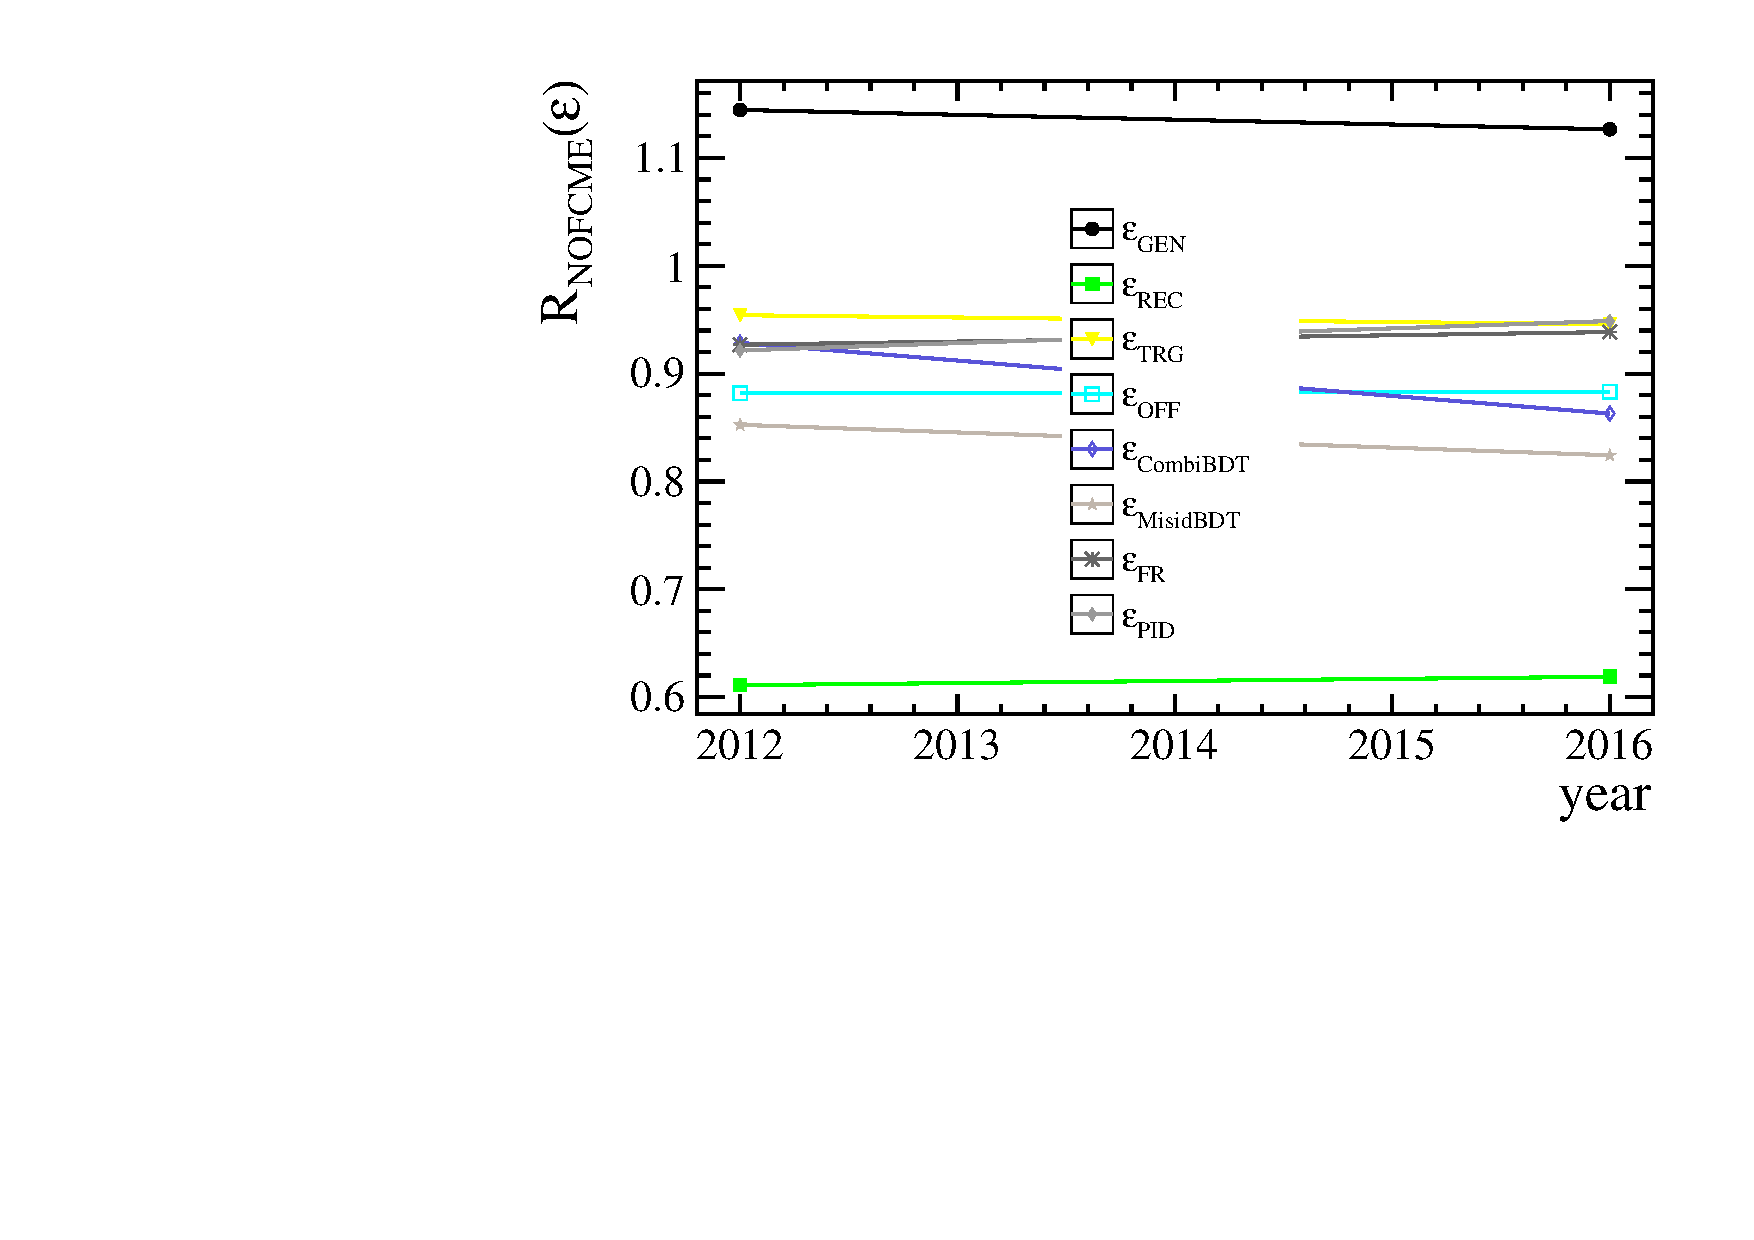
\includegraphics[width = 0.8\textwidth]{efficiency/effiratio/Plot_ALL_Efficiencies_Ratio_Overview_Pretty.pdf}
\caption{Summary of ratio of efficiencies between 2012 simulation and 2016 simulation with no FCME split. Efficiency values for 2016 are TCK-weighted averaged efficiencies.}
\centering
\label{fig:rateffsnofcme}
\end{figure}

%\noindent More detailed discussion on individual efficiencies is covered in following subsections. 


\subsection{Detector Acceptance Efficiency (GEN)}
For charged particles, detector acceptance efficiency describes the fraction of decays contained in the polar angle region of [10, 400] mrad.  
For 2012 and 2016 simulation samples, the overall detector acceptance efficiency will be the average for two possible magnetic polarity conditions. For 2012 this will be also averaged with two different simulation versions: Pythia 6.4\cite{pythia6} and Pythia 8.1\cite{pythia8}.

The hierarchy of generator level efficiencies $\varepsilon^{s}_{GEN} > \varepsilon^{n}_{GEN}$ is expected as the muon is lighter than kaon, making the kaon more likely to be softer and at larger angle, therefore outside of the acceptance. 

%
%        \begin{table}[H]
%                \begin{center}
%        \begin{tabular}{l c c }
%
%%        \hline
%                Channel & Year & $\varepsilon_{gen}$\\ \hline
%              %  $B^{+} \rightarrow J/\psi K^{+}$ & 2011 &  Sim08, Pyth6 & N/A & N/A & \\
%              %  $B^{+} \rightarrow J/\psi K^{+}$ & 2011 &  Sim08, Pyth8 & 0.16379 $\pm$ 0.00030 & 0.16366 $\pm$ 0.00030 & 0.16372$\pm$0.00021 \\
%                \Bmumumu & 2012 & 0.1856$\pm$0.0011 \\
%%                \Bmumumu & 2012 & \\
%                \Bmumumu & 2016 & 0.1959$\pm$0.0016 \\ \hline
%
%                \bjpsimumuk & 2012 & 0.1622$\pm$0.0002\\
%                %$B^{+} \rightarrow J/\psi K^{+}$ & 2012 &  \\
%                %$B^{+} \rightarrow J/\psi K^{+}$ & 2015 &  Sim09a, Pyth8 & 0.17304 $\pm$ 0.00048 & 0.17386 $\pm$ 0.00047 &0.17346$\pm$0.00034 \\
%                \bjpsimumuk & 2016 &  0.1739$\pm$0.0004  \\
%                \hline
%%               \Bmumumu & 2012 &  Sim08, Pyth6 &0.1828$\pm$0.0015 & \multirow{2}{*}{0.1856$\pm$0.0011} \\
%%                \Bmumumu & 2012 &  Sim08, Pyth8 &0.1884$\pm$0.0015 & \\
%%                \Bmumumu & 2016 &  Sim09b, Pyth8 &0.1959$\pm$0.0016 & 0.1959$\pm$0.0016 \\
%              %  $B^{+} \rightarrow J/\psi \pi^{+}$ & 2012 &  Sim08, Pyth6 & 0.1519 $\pm$ 0.000400 & N/A & \multirow{2}{*}{0.15816$\pm$0.00024}\\
%              %  $B^{+} \rightarrow J/\psi \pi^{+}$ & 2012 &  Sim08, Pyth8 & 0.1622 $\pm$ 0.000424 & 0.1611 $\pm$ 0.000421 &  \\
%%               \hline
%              %  $B^{0} \rightarrow J/\psi K^{*}$ & 2012 &  Sim08, Pyth8 & 0.16141 $\pm$ 0.00043 & 0.16050 $\pm$ 0.00043 &0.16095$\pm$0.00030 \\
%%                \hline
%              %  PartReco & 2012 & Sim08, Pyth8 & 0.16058 $\pm$ 0.00051 & 0.16058 $\pm$ 0.00050 & 0.1606$\pm$0.0004 \\
%%                \hline
%                \end{tabular}
%        \end{center}
%        \caption{Geometrical detector acceptance efficiencies for signal and normalisation channel. For 2012 and 2016 simulation samples, the overall detector acceptance efficiency will be the average for two possible magnetic polarity conditions: down, up. For 2012 this will be also averaged with two different simulation versions: Pythia 6.4\cite{pythia6} and Pythia 8.1\cite{pythia8}.}%  Efficiencies were calculated by generating statistics tables generated using dirac-bookeeping-prod4path, looking at generator level cut efficiency: /afs/cern.ch/user/s/slstefko/cmtuser/stattables.}
%        \label{tab:MCdeteff}
%        \end{table}

\subsection{Reconstruction Efficiency (REC)}
The reconstruction efficiency is calculated on simulated events which have passed the detector acceptance. For signal, this efficiency consists of reconstruction and stripping, detailed in~\autoref{tab:stripcutsB}. For normalisation it consists from reconstruction, stripping, \textbf{and on top} the signal stripping is applied. This is done so that selections in normalisation and signal channel are kept as similar as possible and the fact that the signal selection has tighter cuts as explained in~\autoref{nchannel}. However, it should be noted that reconstruction efficiency reflects stripping selection \textbf{without the PID cuts} for both signal and normalisation. This is because \gls{PID} is badly modelled in simulation and hence will be accounted for separately and at the end of the selection chain.

The hierarchy of reconstruction level efficiencies $\varepsilon^{s}_{REC} < \varepsilon^{n}_{REC}$ is also expected as many variables in a signal stripping are based on alignment of the mother $B$ with its daughters. For fully reconstructed normalisation channel this is expected to be the case, whereas for not fully reconstructed decays the alignment requirement make the selection tighter. 

%  \begin{table}[H]
%                \begin{center}
%        \begin{tabular}{l c c }
%
%    %    \hline
%		Channel & Year & $\varepsilon_{rec|sel}$ \\ \hline
%                \Bmumumu & 2012 &  0.10841$\pm$0.00030 \\
%                \Bmumumu & 2016 &  0.12417$\pm$0.00032 \\ \hline
%                \bjpsimumuk & 2012 & 0.17741$\pm$0.00013 \\ \
%%$B^{+} \rightarrow J/\psi K^{+}$ & 2015 &  Sim09a, Pyth8 & 4201997 & & \\
%                \bjpsimumuk & 2016 &  0.20031$\pm$0.00011 \\
%		
%		\hline
%        \end{tabular}
%        \end{center}
%        \caption{Reconstruction and preselection efficiencies for signal and normalisation channels.}
%        \label{tab:myreco}
%        \end{table}


\subsection{Trigger Efficiency (TRG)}
\label{trigef}
 The trigger efficiency is calculated on top of the (GEN) and (REC) efficiency. In order to extract the trigger efficiency, full simulation for both signal and normalisation is used. It should be noted though that at \gls{LHCb}, full simulation is produced based on a certain trigger configuration. The trigger configuration key, TCK, represents a unique code for exact conditions the data have been triggered with at \texttt{L0}, \texttt{HLT1} and \texttt{HLT2}, notably thresholds of certain quantities such as $p$ and $p_{T}$. 
 
Therefore, if default TCK for simulation is representative for the whole considered dataset, then the efficiency can be extracted directly from the simulation produced, which is the case for the Run \Rn{1} data.

However in Run \Rn{2}, the trigger thresholds have been changing often resulting in 16 different TCKs with very different $p$ and $p_{T}$ thresholds, see Table ~\autoref{tab:2016MC} for full details. In the second column, luminosity proportion for 2016 is given. It can be seen that the default simulation in 2016 (corresponding to TCK decimal key 288888335) only represents around 35\% of the data. For this reason, the trigger efficiencies for 2016 data have been obtained by emulation of the trigger on simulation for \texttt{L0} and \texttt{HLT1} level for each individual TCK, creating 16 TCK-based simulations.  This trigger emulation to extract efficiencies was tested with the default trigger configuration (TCK 288888335) to validate the emulation and the correct efficiencies have been recovered. It should be noted that small differences arise from difference between \textit{offline} and \texttt{HLT1} container for \gls{PV}s which stores the information about \gls{minipchi2} as the \gls{PV} finding-algorithm is different, but these have negligible effect. %\mybox{mentioning this just for reproducibility, but maybe not necessary}.
%Therefore the emulation will not be exact, however, the effect is very small as it seems to be only resolution that will slightly shift the distribution, see figure ~\autoref{fig:hlt1shortcoming} 

In order to obtain the average efficiency for Run \Rn{2}, the 16 TCK efficiencies are weighted by the proportion of luminosity corresponding to the integrated luminosity for a given TCK over the full 2016 integrated luminosity.
%The integrated luminosity per TCK was extracted by looking at API version of the \gls{LHCb} run database. 

The full trigger efficiency for Run \Rn{2} is calculated by averaging the luminosity-weighted efficiencies, as seen in ~\autoref{tab:L0andHLT1Calib}. This TCK-dependant luminosity-weighted average efficiency is going to be given as a final efficiency for Run \Rn{2} from now on for all subsequent efficiencies unless stated otherwise.  
%Given that trigger efficiencies for Run \Rn{2} are TCK-dependant, luminosity-weighted average are calculated from now on for all the efficiencies.

\begin{table}
	\begin{center}
		%\small
      \begin{tabular}{l H l l | l l l l | l l }\toprule
      \multicolumn{4}{c |}{ } & \multicolumn{4}{c|}{\texttt{HLT1TrackMuon}} & \multicolumn{2}{c}{\texttt{L0Muon}}\\ \hline
	      TCK dec & TCK hex & \%$\mathcal{L}$ & $\mathcal{L}$ & \gls{pgh2} & $p_{\mu}$ & $p_T(\mu)$ & \gls{minipchi2} & $SPD$ & $p_T(\mu)$\\% & $sum_{ET}$\\
	      &  & \% & $\textrm{pb}^{-1}$ & & [\mev] & [\mev] &  & & [\mev] \\ \hline% & $sum_{ET}$\\
      \multicolumn{10}{c}{\textbf{2016 MD} $0.86\,\textrm{fb}^{-1}$} \\ \hline 
      287905280 & 0x11291600 & $0.8$ & $12.7$  & $-$ & 6.0 & 0.91 & 10        & 450  & 14 \\% &  $-$\\
      287905283 & 0x11291603 & $2.1$ & $35.0$  & $-$ & 6.0 & 0.91 & 10         & 450  & 23 \\% &  $-$ \\
      287905284 & 0x11291604 & $1.5$ &  $24.8$  & $-$ & 6.0 & 0.91 & 10        & 450  & 27 \\% & $-$ \\
      287905285 & 0x11291605 & $4.7$ &   $78.4$   & $-$ & 6.0 & 0.91 & 10      & 450 & 31 \\% & $-$ \\
      288822793 & 0x11371609 & $4.4$   &  $72.1$ & 0.2 & 6.0 & 1.1  & 35       & 450  & 27 \\% & $-$ \\
      288822798 & 0x1137160e & $1.4$  &  $22.8$ & 0.2 & 6.0 & 1.1  & 35       & 450  & 27 \\% & $-$ \\
      288888329 & 0x11381609 & $0.4$  &  $6.9$  & 0.2 & 6.0 & 1.1  & 35       & 450 & 31 \\% & $-$ \\
      288888334 & 0x1138160e & $2.0$  &  $31.7$  & 0.2 & 6.0 & 1.1  & 35      & 450 & 31 \\% & $-$ \\
      288888335 & 0x1138160f & $34.7$  &  $575.3$  & 0.2 & 6.0 & 1.1  & 35  & 450 & 37 \\ \hline% & $-$ \\
      \multicolumn{10}{c}{\textbf{2016 MU} $0.80\,\textrm{fb}^{-1}$} \\ \hline
      288495113 & 0x11321609 & $6.5$ &  $107.0$   &  $-$ & 6.0 & 0.91 & 10 & 450 & 27 \\% & $-$   \\
      288626185 & 0x11341609 & $7.1$ &  $118.1$  &  $-$ & 6.0 & 0.91 & 10 & 450 & 27 \\% & $-$    \\
      288691721 & 0x11351609 &  $1.4$ &  $23.5$   &  0.2 & 6.0 & 1.1  & 35  & 450 & 27 \\% & $-$  \\
      288757257 & 0x11361609 & $25.0$ &  $414.6$   &  0.2 & 6.0 & 1.1  & 35 & 450 & 27  \\% & $-$   \\
      288888337 & 0x11381611 & $ 2.7$ &  $44.1$  &  0.2 & 6.0 & 1.1  & 35  & 450 & 31 \\% & $-$   \\
      288888338 & 0x11381612 & $5.4$ &  $89.8$  &  0.2 & 6.0 & 1.1  & 35  & 450 & 33 \\% & $-$    \\
      288888339 & 0x11381613 & $0.1$ &  $1.1$  &  0.2 & 6.0 & 1.1  & 35  & 450 & 27 \\ \hline% & 1000 \\
      \multicolumn{10}{c}{\textbf{Default Simulation}} \\ \hline
      1362630159 & 0x5138160f & $-$  & $-$   & 0.2 & 6.0 & 1.1  & 35 & 450 & 37\\% &  157\\
     \bottomrule
   \end{tabular}
\caption{Summary of 16 different TCKs listing properties of candidates necessary to pass \texttt{L0} and \texttt{HLT1} selection in 2016. In the final row, the default configuration for 2016 is shown and it corresponds to 288888335 TCK.}
\label{tab:2016MC}
	\end{center}
\end{table}

For the \texttt{HLT2} level, there were no significant changes of thresholds and hence efficiencies are obtained from full simulation regardless. The systematic effect of this assumption will be listed in~\autoref{systematics}.




%As it can be seen in the list of trigger requirements in ~\ref{tab:triggersel}, \texttt{L0MuonDecision} needs to be modelled. This trigger line selects event candidates only if candidate has certain muon $p_{T}$ and $nSPD$ hits.


%\texttt{HLT1} trigger selection was also emulated offline as \texttt{HLT1}. The efficiency of \texttt{HLT1TrackMuonDecision} is then determined on the top of \texttt{L0MuonDecision} as only events which have passed either \texttt{L0MuonDecision} or \texttt{L0DimuonDecision} would be considered. \texttt{HLT1TrackMuonDecision} trigger lines requires events with only certain muon $p_{T}$,$p$, \textit{ghost probability} and $MIP\chi^{2}$. 

%There are other variables that are included in \texttt{HLT1TrackMuonDecision} such as whether the track is \gls{VELO} track or how many hits have been missed in \gls{VELO}, however, these have not changed throughout the Run \Rn{2} data and are not likely to be different between signal and normalisation channel.  Hence only efficiency for the relevant cuts are included in emulation of \texttt{HLT1TrackMuonDecision}.

%It should be noted that there is difference between \textit{offline} and \texttt{HLT1} container for PVs which stores the information about $MIP\chi^{2}$ fast Kalman fitter rather then full is used. Therefore the emulation will not be exact, however, the effect is very small as it seems to be only resolution that will slightly shift the distribution, see figure ~\autoref{fig:hlt1shortcoming}.

%This trigger emulation to extract efficiencies was tested with the default trigger configuation to validate the emulation and the correct efficiencies have been recovered. TCK dependent efficiecy breakdown for signal and normalisation channel can be seen in Table ~\autoref{tab:L0andHLT1Calib}. In order to obtain the average efficiency for Stripping 26, these efficiencies are weighted by the \% of lumi for which this luminosity was ran on. These numbers have been obtained by looking at API version of the rundatabase where one can obtain luminosity per TCK.


\begin{table}[H]
%\small
\begin{center}
\begin{tabular}{ l |  c  c  c | c  c  c }\toprule
	\multicolumn{1}{c|}{} & \multicolumn{3}{c|}{\Bmumumu } & \multicolumn{3}{c}{\bjpsimumuk} \\ \hline
 TCK & $\varepsilon_{L0}$ & $\varepsilon_{HLT1}$ & $\varepsilon_{HLT2}$ & $\varepsilon_{L0}$ & $\varepsilon_{HLT1}$ & $\varepsilon_{HLT2}$ \\
\hline
287905280 & 0.921 & 0.999 & 0.831 & 0.891 & 0.997 & 0.943 \\
287905283 & 0.905 & 0.999 & 0.845 & 0.878 & 0.998 & 0.953 \\
287905284 & 0.894 & 0.999 & 0.855 & 0.867 & 0.998 & 0.962 \\
287905285 & 0.88 & 0.999 & 0.868 & 0.854 & 0.998 & 0.973 \\
288495113 & 0.894 & 0.999 & 0.855 & 0.867 & 0.998 & 0.962 \\
288626185 & 0.894 & 0.999 & 0.855 & 0.867 & 0.998 & 0.962 \\
288691721 & 0.894 & 0.957 & 0.873 & 0.867 & 0.94 & 0.965 \\
288757257 & 0.894 & 0.957 & 0.873 & 0.867 & 0.94 & 0.965 \\
288822793 & 0.894 & 0.957 & 0.873 & 0.867 & 0.94 & 0.965 \\
288822798 & 0.88 & 0.957 & 0.886 & 0.854 & 0.941 & 0.976 \\
288888329 & 0.894 & 0.957 & 0.873 & 0.867 & 0.94 & 0.965 \\
288888334 & 0.88 & 0.957 & 0.886 & 0.854 & 0.941 & 0.976 \\
288888335 & 0.848 & 0.958 & 0.911 & 0.821 & 0.941 & 0.999 \\
288888337 & 0.88 & 0.957 & 0.886 & 0.854 & 0.941 & 0.976 \\
288888338 & 0.871 & 0.957 & 0.895 & 0.844 & 0.941 & 0.984 \\
288888339 & 0.89 & 0.957 & 0.877 & 0.864 & 0.94 & 0.968 \\
\hline
Weighted efficiency & 0.876 & 0.967 & 0.884 & 0.849 & 0.953 & 0.978 \\
\bottomrule
\end{tabular}
\end{center}
\caption{Efficiencies of 2016 trigger emulation on simulation. Depending on TCK, the efficiencies vary up 10\% for \texttt{L0} level for signal simulation and up to 5\% for normalisation TCK. This is important as \textit{single event sensitivity} is sensitive to the ratio of these two efficiencies. This configuration is describing correctly only 35\% data with a high $p_{T}$ threshold.}
\label{tab:L0andHLT1Calib}
\end{table}



Run \Rn{1} trigger efficiency is determined directly by looking at default TCK as it is representative of the whole dataset.% and is summarised in Table ~\autoref{tab:L0andHLT1Calib2012}. 

%It should be noted that in the rest of the efficiencies Stripping 21 with be representative of 21+21r1 dataset as it was noticed that for normalisation channel these efficiencies are eqvivalent. In this section following ratio will be calculated,


%\begin{table}[H]
%\begin{center}
%\begin{tabular}{ l  l  l  l  }
% Efficiency &  \Bmumumu  (2012)  &  \bjpsimumuk (2012) & \bjpsimumuk (2011) \\
%\hline
%$\varepsilon_{L0}$ &0.900 & 0.873 & 0.907 \\
%$\varepsilon_{HLT1}$ &0.934 & 0.908 & 0.879 \\
%$\varepsilon_{HLT2}$ &0.883 & 0.981 & 0.973 \\
%\hline
%\end{tabular}
%\end{center}
%\caption{2012 default TCK efficiencies. These values will be taken to be representative of 2012 and 2011 dataset as the cummulative efficiency for 2011 and 2012 is nearly identical.}
%\label{tab:L0andHLT1Calib2012}
%\end{table}


\subsection{Offline Selection (OFF)}

In this section offline efficiencies are discussed. These include the $J/\psi$ and $\Psi(2S)$ veto signal efficiency that were mentioned in~\autoref{tab:vetoes}, where 2946.0\mevcc $<$ $|$ M($\mu^{+}$ $\mu^{-}$) $|$ $<$ 3176.0\mevcc and 3586.0\mevcc $<|$ M($\mu^{+}$ $\mu^{-}$) $|$ $<$ 3766.0\mevcc. For the normalisation channel this is not applicable as the normalisation decay proceeds via the $J/\psi$ resonance.
%Given that trigger efficiencies for Run \Rn{2} are TCK-dependant, luminosity-weighted average are calculated from now on for all the efficiencies.
%Similarly for all 2016 efficiencies from now on that are calibrated from the simulation are weighted averages, unless stated otherwise.

%\begin{table}[H]
%\begin{center}
%\begin{tabular}{ l c  c  c }
%Efficiency & Year &  \Bmumumu  &  \bjpsimumuk \\
%\hline
%$\varepsilon_{c\bar{c}}$ & 2012  &0.882 & N/A \\
%$\varepsilon_{c\bar{c}}$ & 2016  &0.883 & N/A \\
%\hline
%\end{tabular}
%\end{center}
%\caption{Efficiency of $J/\psi$ and $\Psi(2S)$ veto selections.}
%\end{table}

\subsection{Combinatorial BDT and Misid BDT Efficiency}
 Efficiencies of the MVA selection are evaluated on simulation samples. These efficiencies are obtained using samples that passed (GEN), (REC), (TRG) and (OFF) cuts. The specific MVA for combinatorial background suppression (see ~\autoref{CombiBDTsel}) and misID background suppression (see ~\autoref{misidbdt}) are applied to the simulation samples. As the optimisation led to different BDTs depending on the data-taking period, these are then applied parametrically to the relevant simulation samples. The efficiency results are listed in~\autoref{tab:effsumarry}.

For the Misid and Combinatorial BDT selection, the normalisation \bjpsimumuk channel retains more signal than the \Bmumumu channel. This is due to the kaon/muon $p$ and $p_{T}$ kinematics difference as seen in ~\autoref{fig:reason1} and ~\autoref{fig:reason2}, where the kaon track is generally harder than the muon track. Kaon reconstruction efficiency is worse than muon reconstruction efficiency because about 11\% of the kaons cannot be reconstructed due to hadronic interactions that occur before the last T station~\cite{LHCb-DP-2013-002}, implying that the $p_{T}$ of the $B$ meson is on average harder for the normalisation channel. As these two quantities are high in BDT importance ranking as mentioned in~\autoref{CombiBDTsel}, this makes  the normalisation simulation more efficient. In the Misid BDT selection, again the kinematics of the $B$ meson and the \gls{minipchi2} of the oppositely charged muon to $B$ has a better separation from background than the signal.

%\begin{table}[H]
%\begin{center}
%\begin{tabular}{ l c  c  c }
%Efficiency & Year & \Bmumumu  &  \bjpsimumuk \\
%\hline
%$\varepsilon_{CombiBDT}$& 2012 &0.473 & 0.509 \\
%$\varepsilon_{MisidBDT}$& 2012 &0.436 & 0.511 \\
%\hline
%$\varepsilon_{CombiBDT}$& 2016 &0.343 & 0.397 \\
%$\varepsilon_{MisidBDT}$& 2016 &0.368 & 0.446 \\	
%\hline
%\end{tabular}
%\end{center}
%\caption{2016 Combinatorial and Misid BDT selection efficiency.}
%\label{tab:CombinatorialBDT2012}
%\end{table}


\begin{figure}[H]
\center
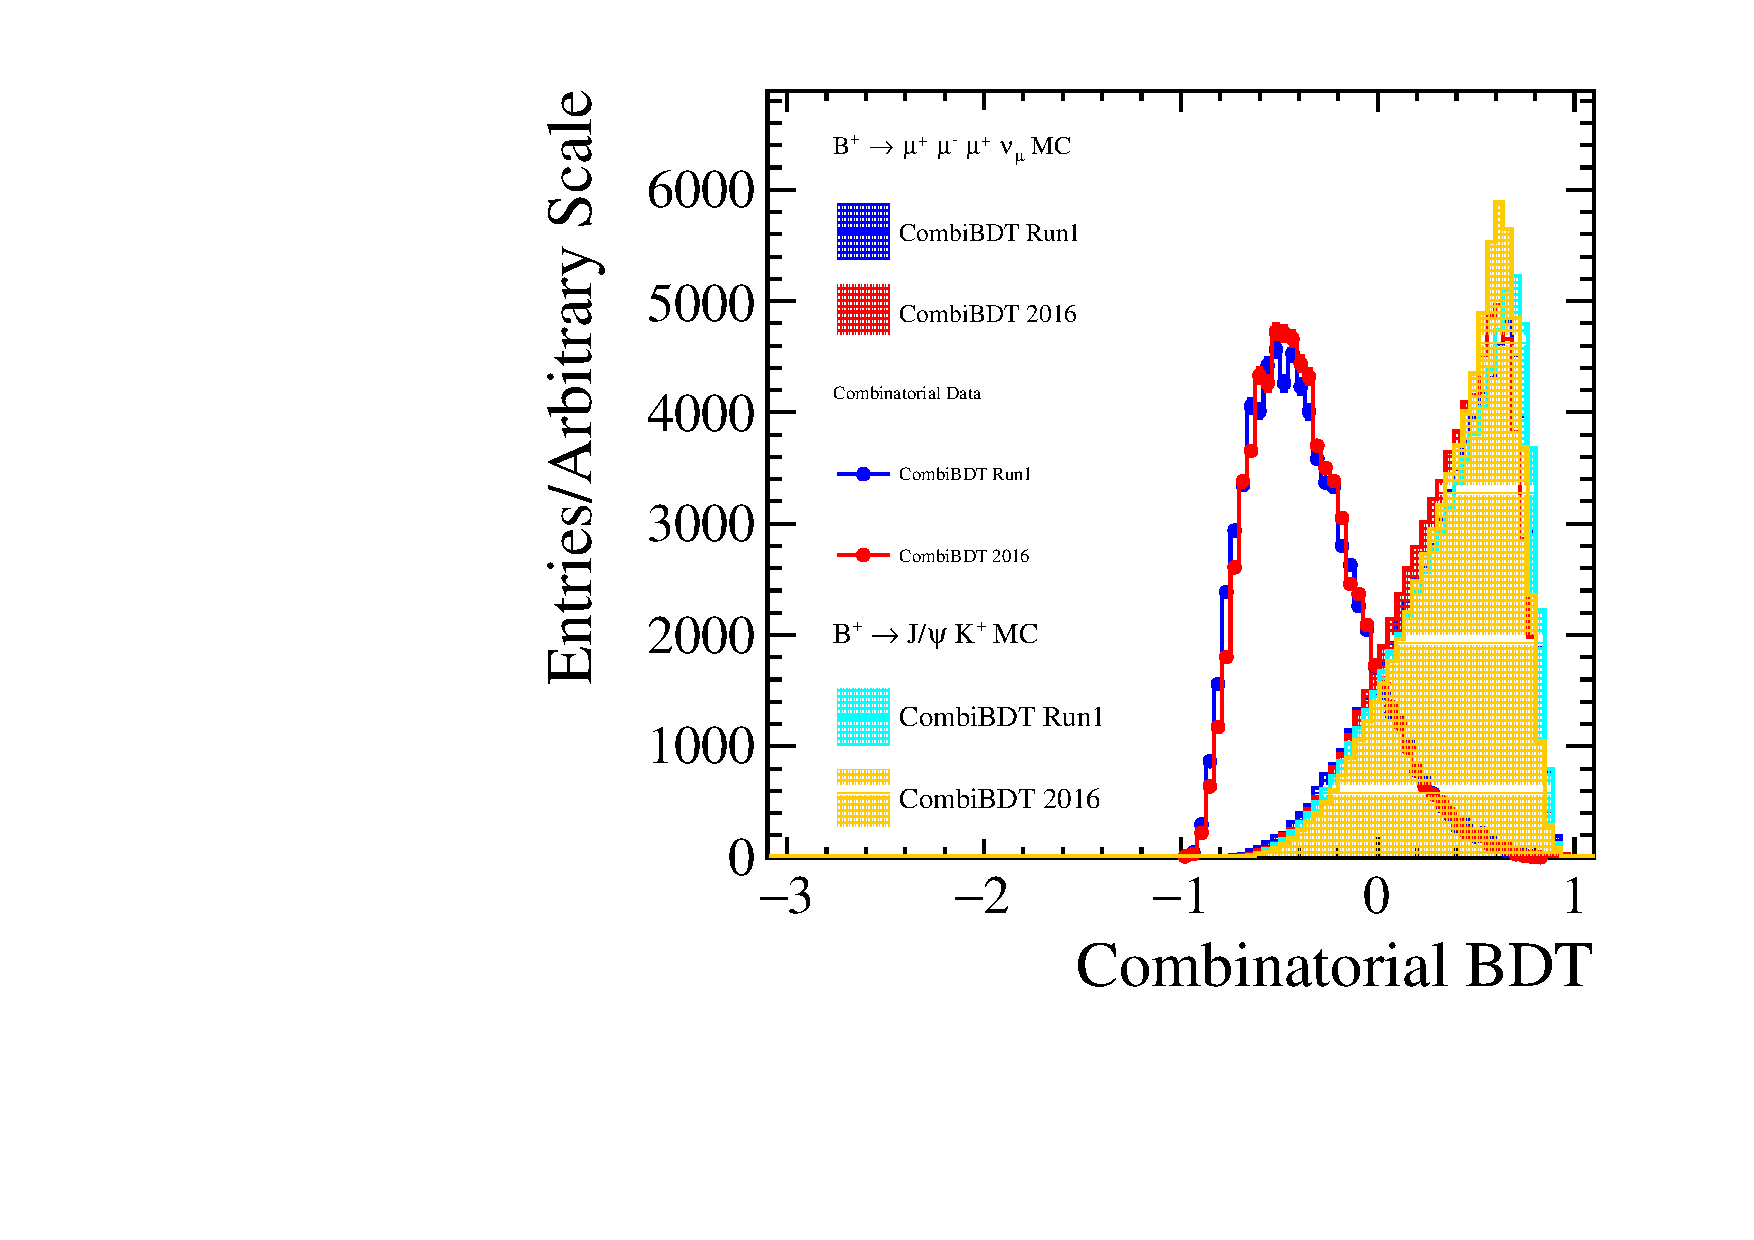
\includegraphics[width = 0.45\textwidth]{efficiency/plot_shapes_before_combibdt_forefficiency/plotvariableCombiBDTNICEFOREFF}\put(-110,133){(a)}%
\includegraphics[width = 0.45\textwidth]{efficiency/plot_shapes_before_combibdt_forefficiency/plotvariableB_PTNICEFOREFF}\put(-110,133){(b)}%
\newline
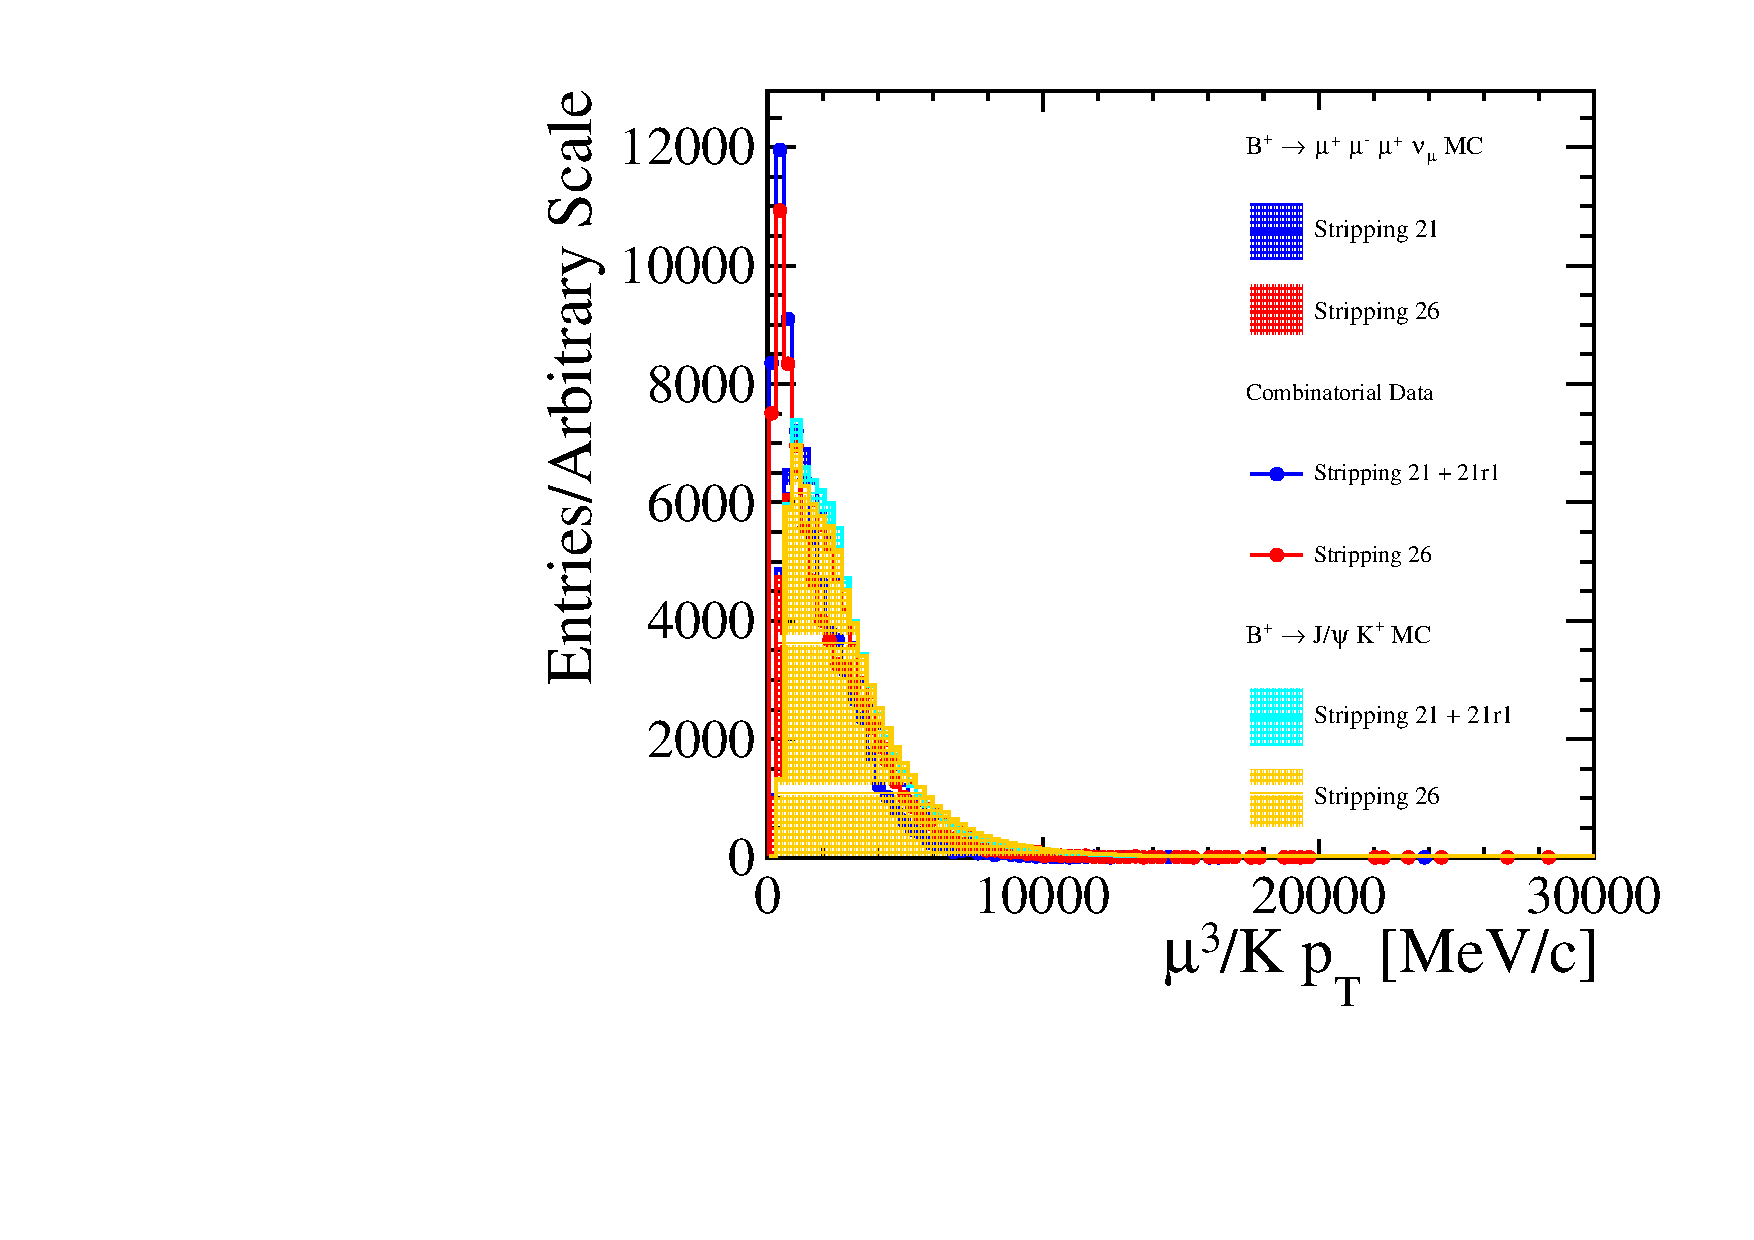
\includegraphics[width = 0.45\textwidth]{efficiency/plot_shapes_before_combibdt_forefficiency/plotvariablemu3_PTNICEFOREFF}\put(-110,133){(c)}%
\includegraphics[width = 0.45\textwidth]{efficiency/plot_shapes_before_combibdt_forefficiency/plotvariablemu3_PNICEFOREFF}\put(-110,133){(d)}%
\caption{(a) Combinatorial BDT response for signal simulation and upper mass sideband as well as for normalisation channel simulation for Stripping 21 and Stripping 26. The most discriminative variables are (b) $p_{T}$ of the $B$ meson, (c) muon/kaon $p_{T}$ and (d) muon/kaon $p$.}
\label{fig:reason1}
\end{figure}

\begin{figure}[H]
\center
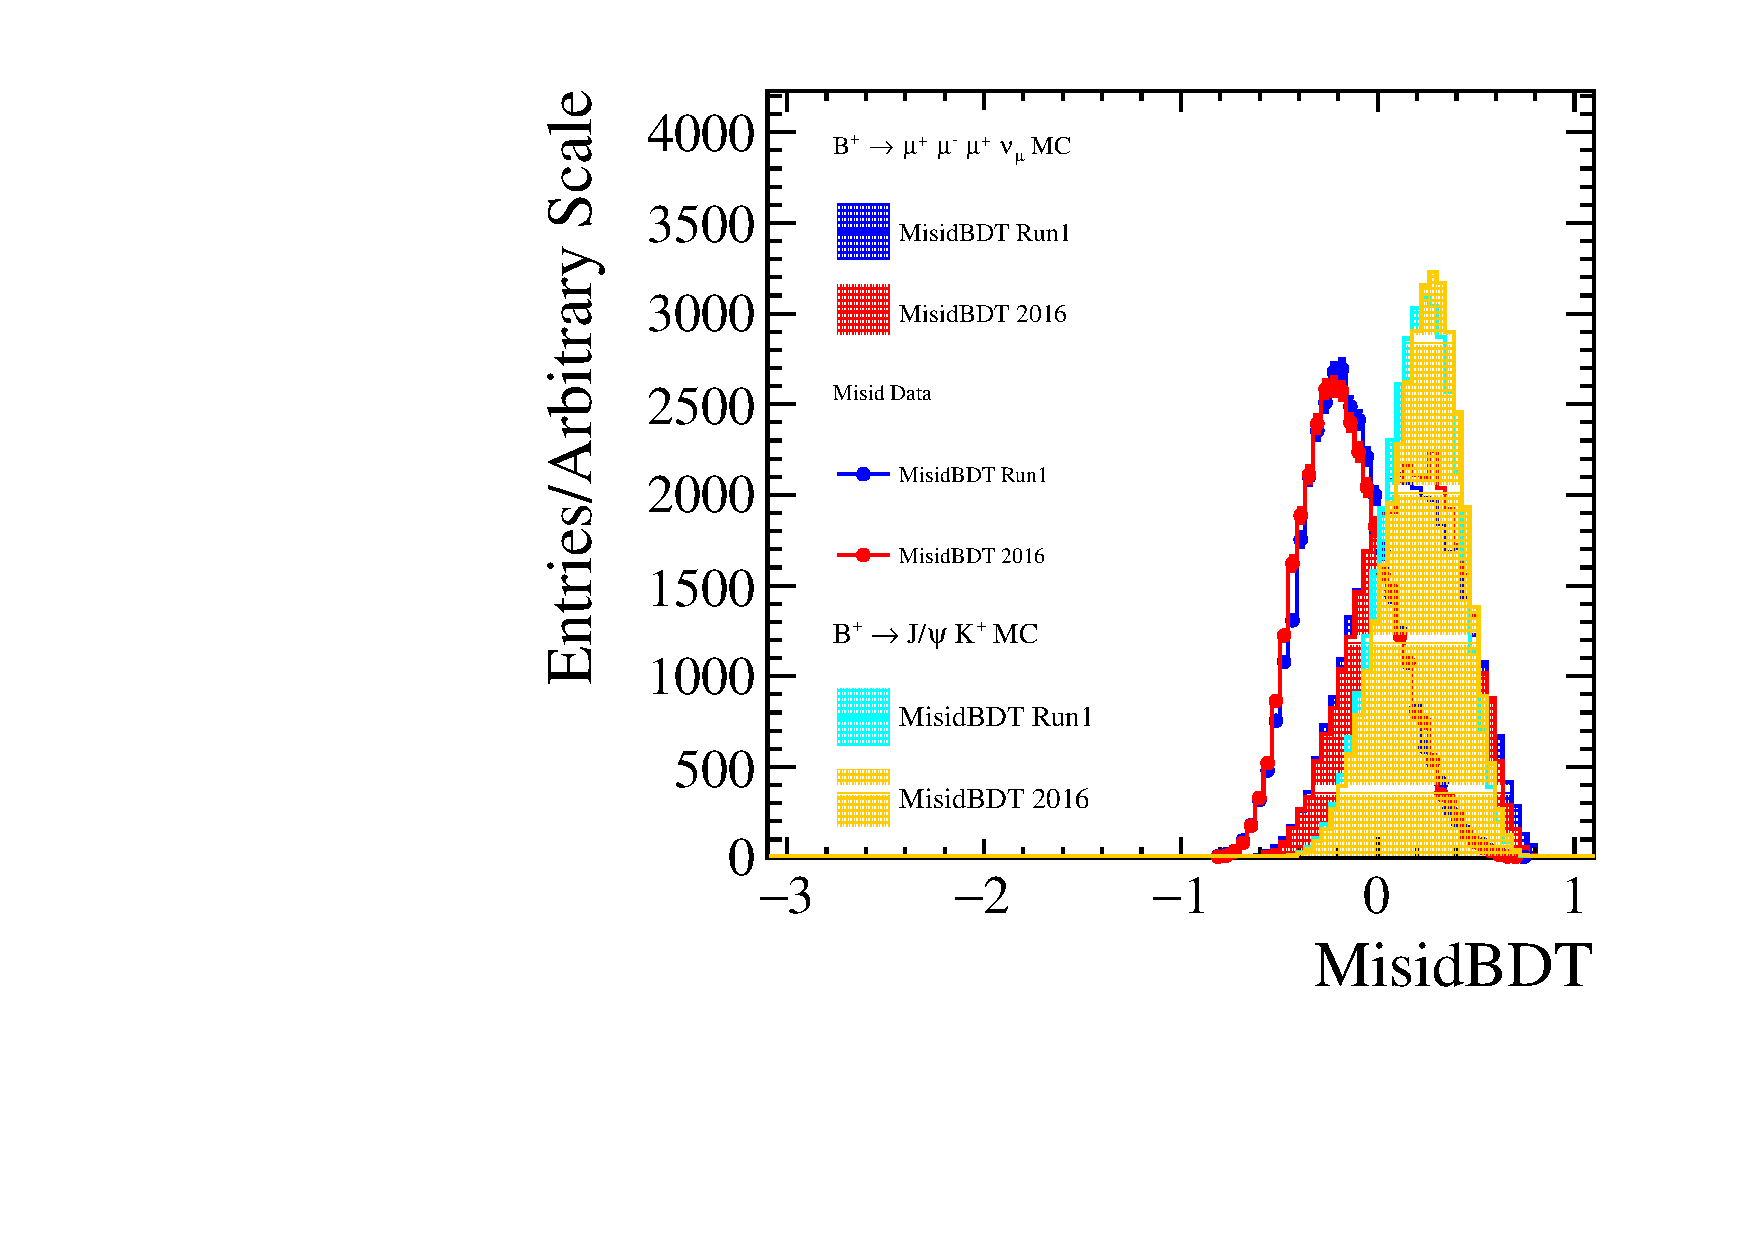
\includegraphics[width = 0.45\textwidth]{efficiency/plot_shapes_before_misidbdt_forefficiency/plotvariableMisidBDTNICEFOREFF}\put(-110,133){(a)}%
\includegraphics[width = 0.45\textwidth]{efficiency/plot_shapes_before_misidbdt_forefficiency/plotvariableB_PTNICEFOREFF}\put(-110,133){(b)}%
\newline
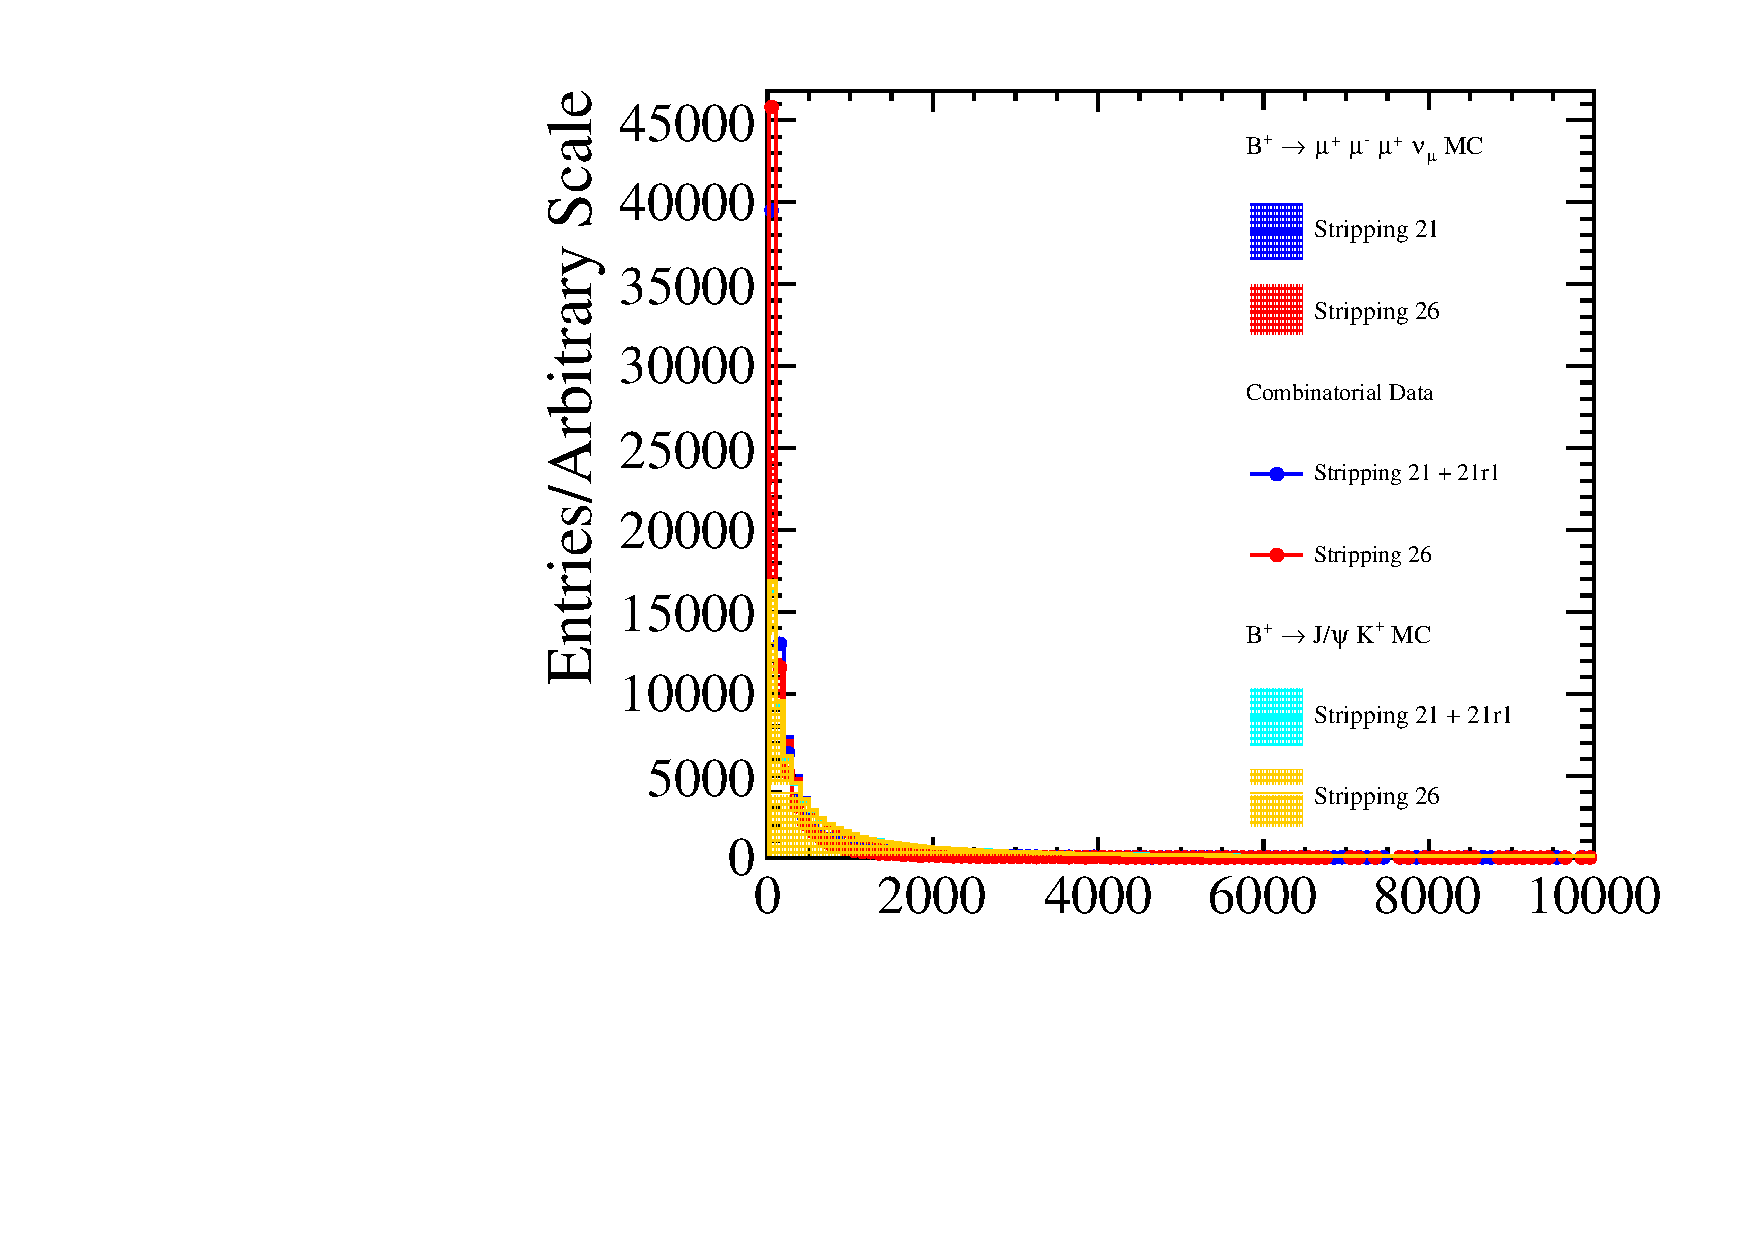
\includegraphics[width = 0.45\textwidth]{efficiency/plot_shapes_before_misidbdt_forefficiency/plotvariablemu2_MINIPCHI2NICEFOREFF}\put(-110,133){(c)}%
\includegraphics[width = 0.45\textwidth]{efficiency/plot_shapes_before_misidbdt_forefficiency/plotvariablemu3_PNICEFOREFF}\put(-110,133){(d)}%
\caption{(a) Misid BDT response for signal simulation and upper mass sideband as well as for normalisation channel simulation for Stripping 21 and Stripping 26. The most discriminative variables are (b) $p_{T}$ of B, (c) muon IP $\chi^{2}$  and (d) muon/kaon $p$. Misid BDT responses are plotted with combinatorial BDT already applied.}
\label{fig:reason2}
\end{figure}

\subsection{Fitting Range Efficiency (FR)}

As discussed in~\autoref{fittingsel} and in~\autoref{combiback}, the fitting region was chosen in order to avoid modelling a drop in low corrected mass region for the combinatorial background (exclusion below $4000$ \mevcc) and secondly in order to not include a region where there are very few/no events (exclusion above $7000$ \mevcc) in \textbf{corrected mass}. As seen in~\autoref{tab:effsumarry} and in~\autoref{fig:reasonfitrange} the normalisation channel does not loose many candidates compared to the signal channel.
%This is expected as the \textbf{visible mass} is more constrained in normalisation channel from preselection stage (see ~\autoref{tab:stripcutsBnorm}, where $5150\ \mevcc\ <\ B$ Mass$\ <\ 5450\ \mevcc$) than in signal channel as seen in~\autoref{fig:reasonfitrange}). Hence, restricting region in \textbf{corrected mass} is does not affect normalisation channel much.

\begin{figure}[H]
\center
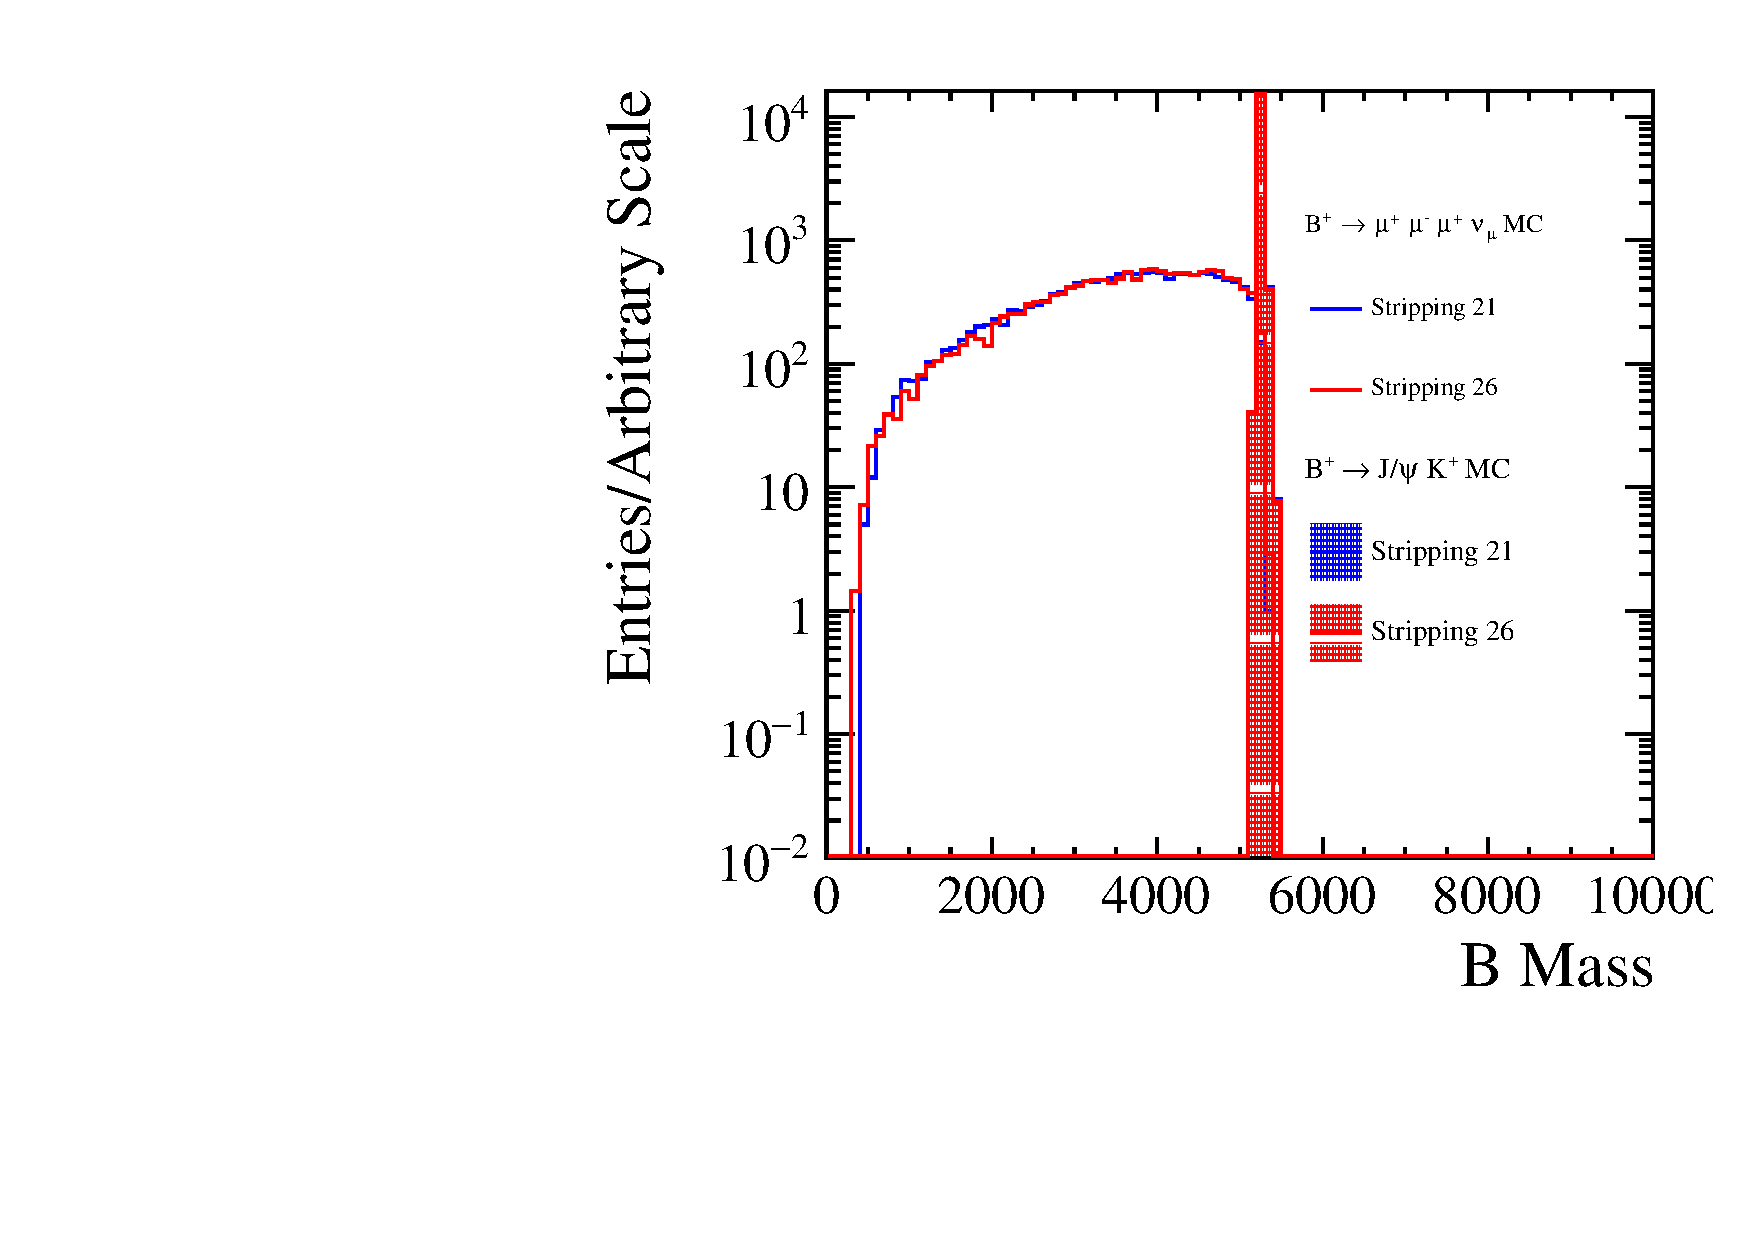
\includegraphics[width = 0.5\textwidth]{efficiency/plot_shapes_fittingregion/plotvariableB_MMMIX.pdf}\put(-110,133){(a)}%
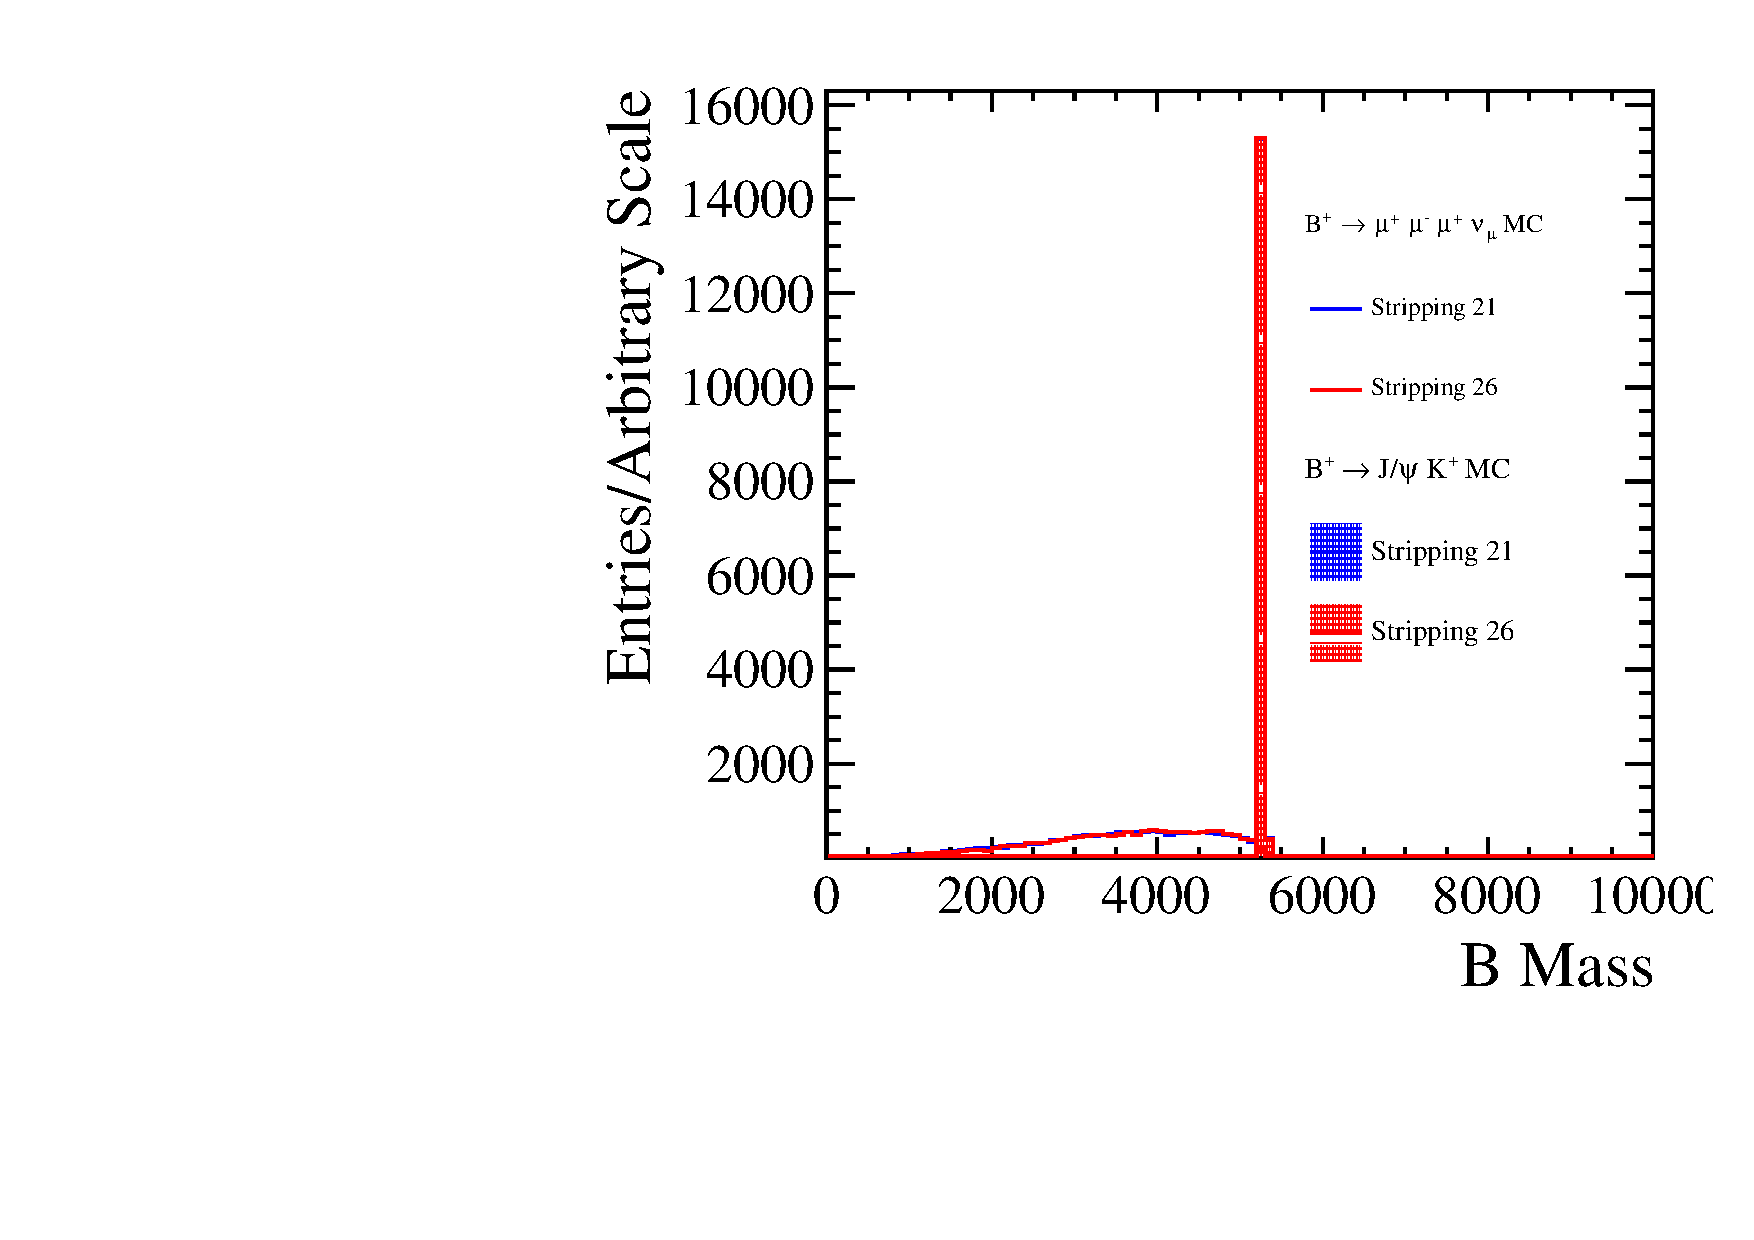
\includegraphics[width = 0.5\textwidth]{efficiency/plot_shapes_fittingregion/plotvariableLogyB_MMMIX.pdf}\put(-110,133){(b)}%
\caption{(a) Visible mass of normalisation and signal simulation. It can be seen that normalisation previous preselection has a sharp cut around $B$ visible mass leading to much higher fitting region efficiency. (b) The corresponding logarithmic version of plot (a).}
\label{fig:reasonfitrange}
\end{figure}


%\begin{table}[H]
%\begin{center}
%\begin{tabular}{ l c  c  c }
%Efficiency & Year &  \Bmumumu  &  \bjpsimumuk \\
%\hline
%$\varepsilon_{FR}$ & 2012  &0.923 & 0.996 \\
%$\varepsilon_{FR}$ & 2016  &0.938 & 0.999 \\
%\hline
%\end{tabular}
%\end{center}
%\caption{Efficiency of fitting range selection.}
%\label{tab:fiteff}
%\end{table}

\subsection{\gls{PID} Efficiencies (PID)}
\label{PIDaff}
As \gls{PID} variables are not correctly modelled in the simulation, mentioned in~\autoref{simulationchap}, a data-driven approach of extracting PID efficiency is taken. To avoid the introduction of any any biases in previous steps, especially in multivariate selection, PID efficiencies are evaluated at the end of the selection chain with the \texttt{PIDCalib} package data samples.

The PID efficiency is higher for the normalisation channel with all PID requirements given in~\autoref{tab:PIDselectionNorm} compared to signal provided in~\autoref{tab:PIDselection} due to weaker PID requirement on the kaon as compared to the muons.

\begin{table}[H]
\begin{center}
\begin{tabular}{l c c}\toprule

%    \begin{tabular}{ | l | c | } %p{7cm}|}
    Species  & 2012 PID Simulation & 2016 PID Simulation\\ \hline
    muon &  DLLmu $ > 0$ & DLLmu $ > 0$ \\
    muon &  (DLLmu - DLLK) $ > 0$ & (DLLmu - DLLK) $ > 0$ \\
    muon &   - & \texttt{IsMuonTight==1.0}\\
    muon &  \texttt{Nshared==0} & \texttt{Nshared<2} \\
	muon &  \texttt{Probnnmu}$>0.35$ & \texttt{Probnnmu}$>0.35$ \\
     \hline
   $\varepsilon_{PID}$   & 0.631$\pm$ 0.005 & 0.623$\pm$0.006 \\

     \bottomrule
      \end{tabular}
\end{center}
\caption{Signal simulation efficiency using \texttt{PIDCalib} efficiencies.}
\label{tab:PIDselection}
\end{table}

\begin{table}[H]
\begin{center}
\begin{tabular}{l c c}\toprule

%    \begin{tabular}{ | l | c | } %p{7cm}|}
    Species  &2012 PID Simulation & 2016 PID Simulation\\ \hline
    muon &  DLLmu $ > 0$ & DLLmu $ > 0$ \\
    muon &  (DLLmu - DLLK) $ > 0$ & (DLLmu - DLLK) $ > 0$ \\
    muon &  - & \texttt{IsMuonTight==1.0}\\
    muon & \texttt{Nshared==0} & \texttt{Nshared<2} \\
    muon & \texttt{Probnnmu}$>0.35$ & \texttt{Probnnmu}$>0.35$ \\
    kaon &  DLLK $ > 0$ & DLLK $ > 0$ \\
    kaon &  (DLLp - DLLK) $ < 5$ & (DLLp - DLLK) $< 5$ \\
%    kaon &  $\Delta LL(K - \pi) > 0$ & $\Delta LL(K - \pi) > 0$ \\
%    kaon &  $\Delta LL(p - K) < 5$ & $\Delta LL(p - K) < 5$ \\
     \hline
    $\varepsilon_{PID}$ &0.685$\pm$ 0.001 & 0.656$\pm$0.001  \\

     \bottomrule
      \end{tabular}

\end{center}
\caption{Normalisation simulation efficiency using \texttt{PIDCalib} efficiencies.}
\label{tab:PIDselectionNorm}
\end{table}


\newpage
\section{Mass Fits}
In this section, firstly the parametrisation of the normalisation channel is shown in~\autoref{normparam}. The fit to the normalisation channel using the full fit model is described in~\autoref{normfit}. This is followed by the signal fit parametrisation outlined in~\autoref{sigpara} resulting in blinded and non-blinded data fits described in~\autoref{fitsens}.

\subsection{Normalisation Channel Parametrisation}
\label{normparam}

The obtain the \bjpsimumuk yield of Run \Rn{1} and Run \Rn{2}, an unbinned extended maximum likelihood fit to the invariant $\mu^{+} \mu^{-} K^{+}$ data distribution in each respective Run is performed. In this section contributions to the normalisation fit model are considered. 
%The \bjpsimumuk decays are very often studies at LHCb and in this particular case, there will be three components to the fit.

\subsubsection{Signal}

	The first component is the signal itself, which is modelled with PID-weighted simulation and can be best described by a double-sided Ipatia function, detailed in~\autoref{IP}, where all the parameters apart from the mean $\mu^{IP}$ and width $\sigma^{IP}$ are fixed from the signal simulations. These simulations pass through the same selection process as the corresponding \bjpsimumuk data, described in~\autoref{nchannel}, with one exception. Instead of directly cutting on \gls{PID} variables, the simulations are reweighted with the relevant \gls{PID} weights, because of the known mismatch between simulation and data. More on this will be covered in~\autoref{PIDaff}. 


\subsubsection{\mb{\bjpsimumupi} Background}

Since the PID requirements on the kaon are very loose, there will be a background contribution from $ B^{+} \rightarrow (J/\psi \rightarrow \mu^{+} \mu^{-}) \pi^{+}$. This contribution is modelled by a double-sided Crystal Ball function to $B^{+} \rightarrow (J/\psi \rightarrow \mu^{+} \mu^{-}) \pi^{+}$ simulation, where the pion track is given the kaon mass hypothesis. Again, all the parameters apart from mean $\mu^{CB}$ and width $\sigma^{CB}$ are fixed from the fit of this simulation. In ~\autoref{fig:FitToPiMuMu}, fits to \bjpsimumuk simulation and \bjpsimumupi simulation from Stripping 21 are showed using different scales.
For signal, Run \Rn{1} Stripping 21 simulation sample is used and for Run \Rn{2} the Stripping 26 - TCK 288888335 simulation sample is used. For the \bjpsimumupi Stripping 21 simulation sample is used for both Run \Rn{1} and Run \Rn{2}.

\begin{figure}[ht]
\centering
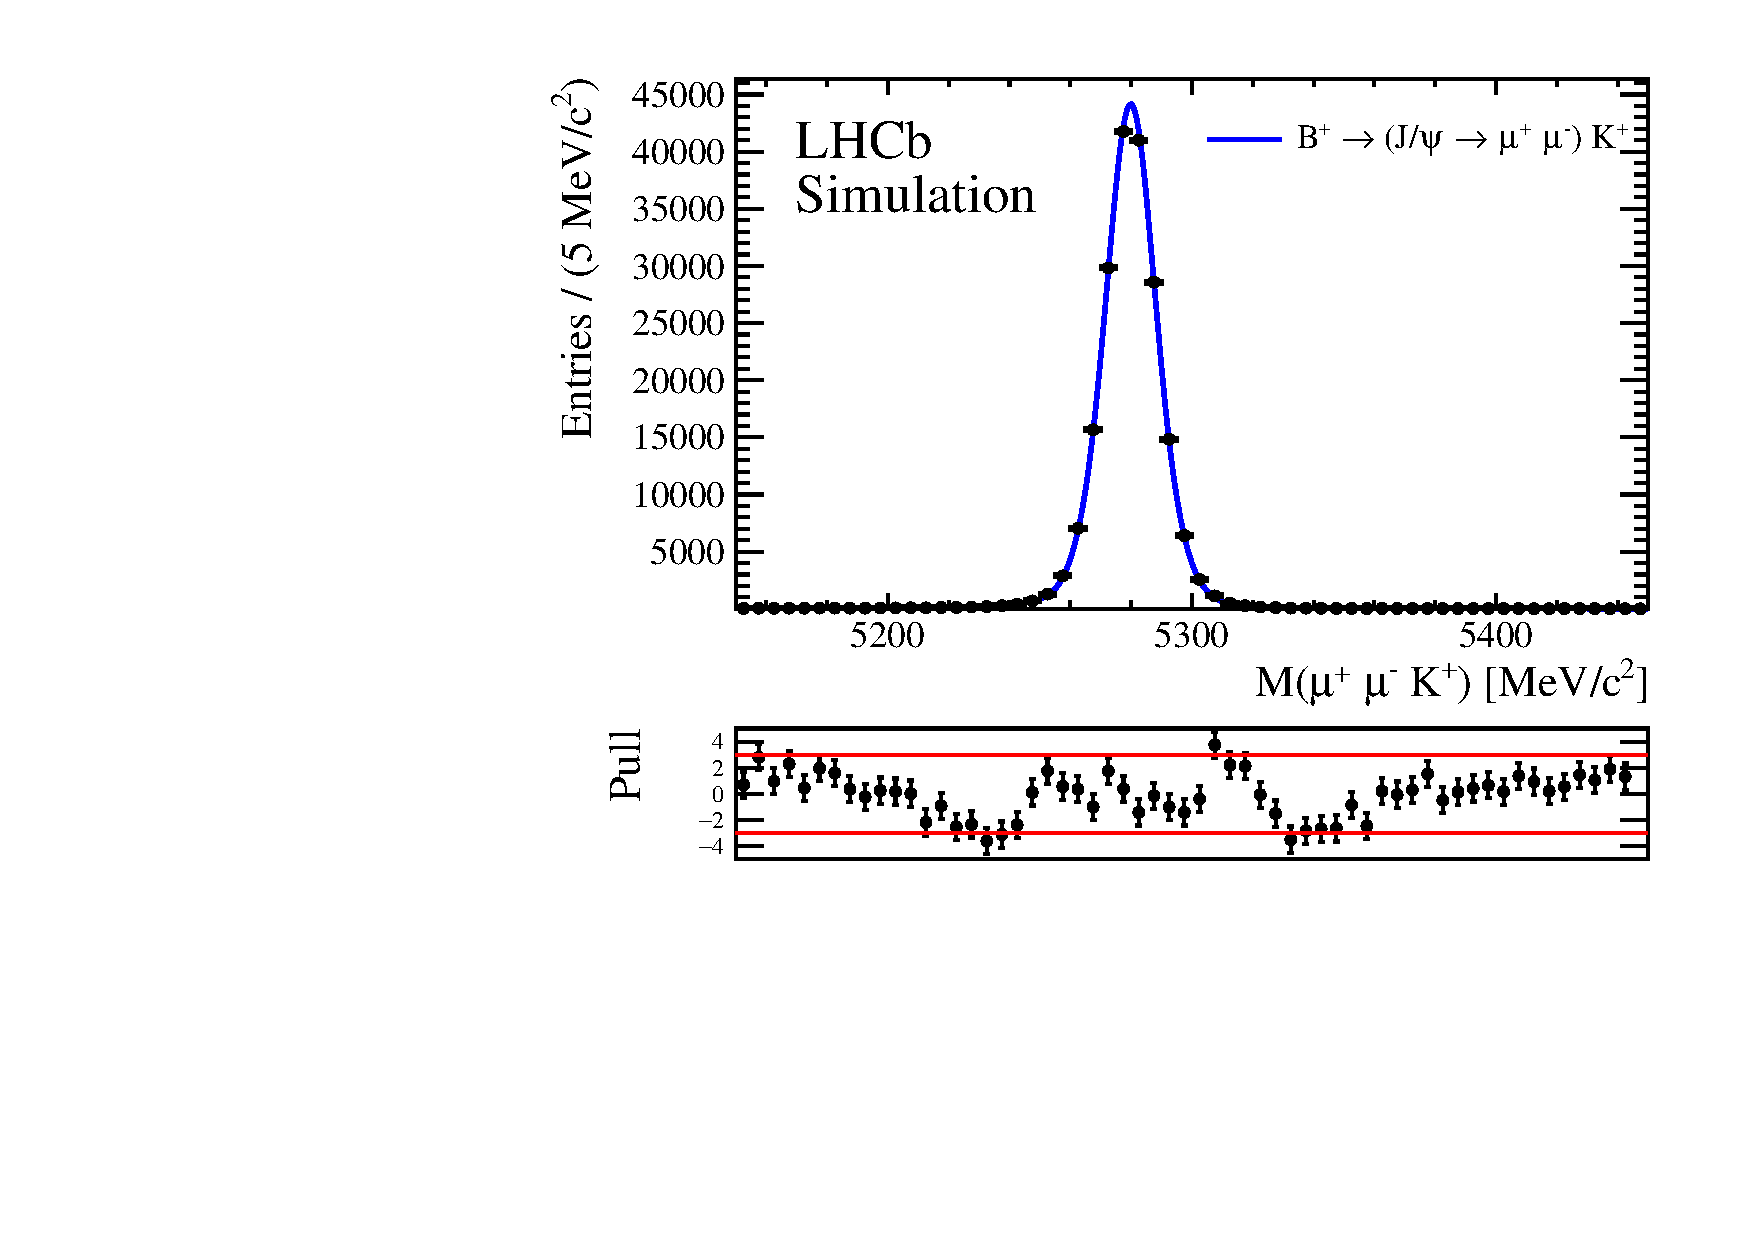
\includegraphics[width=0.45\linewidth]{./efficiency/controlchannelfits/controlsigmcnofcmeRun1nolog.pdf}\put(-50,57){(a)}%
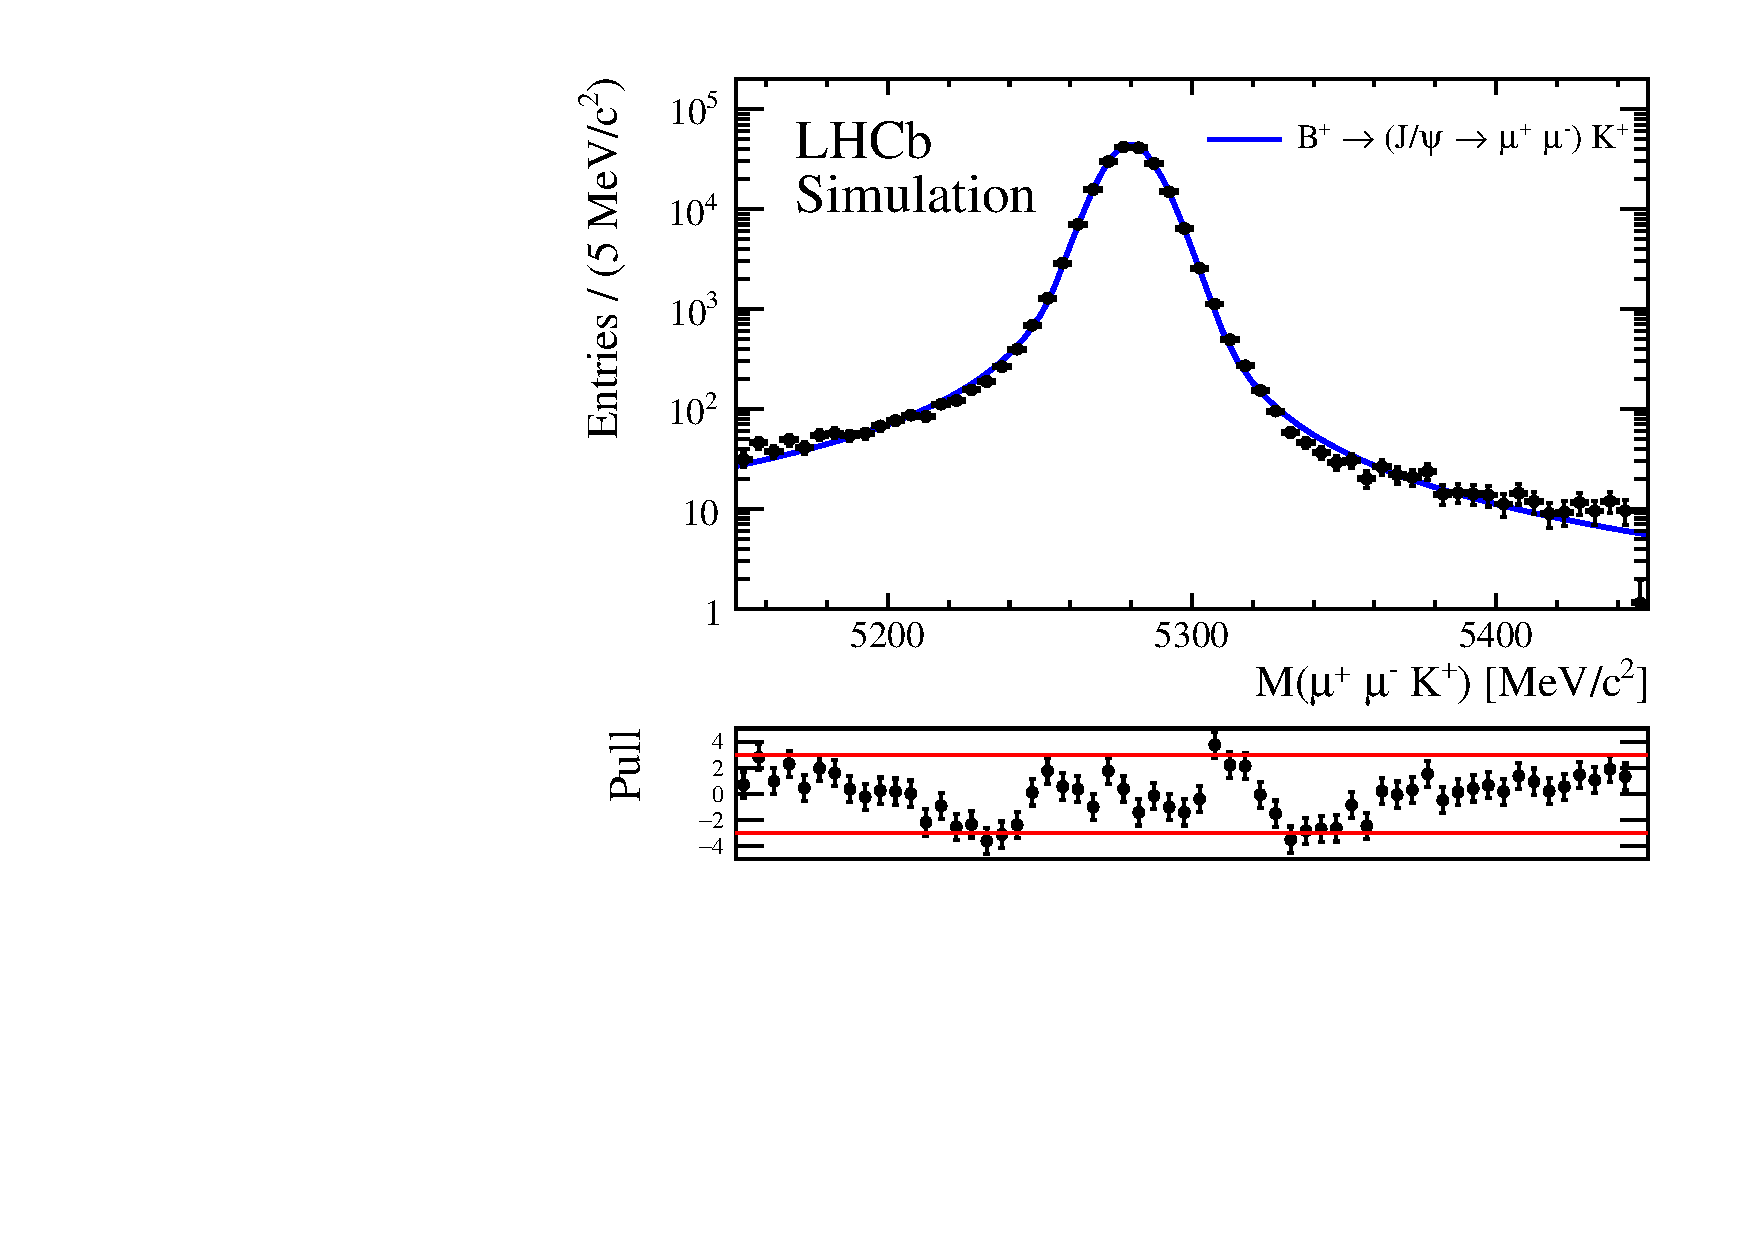
\includegraphics[width=0.45\linewidth]{./efficiency/controlchannelfits/controlsigmcnofcmeRun1log.pdf}\put(-50,57){(b)}


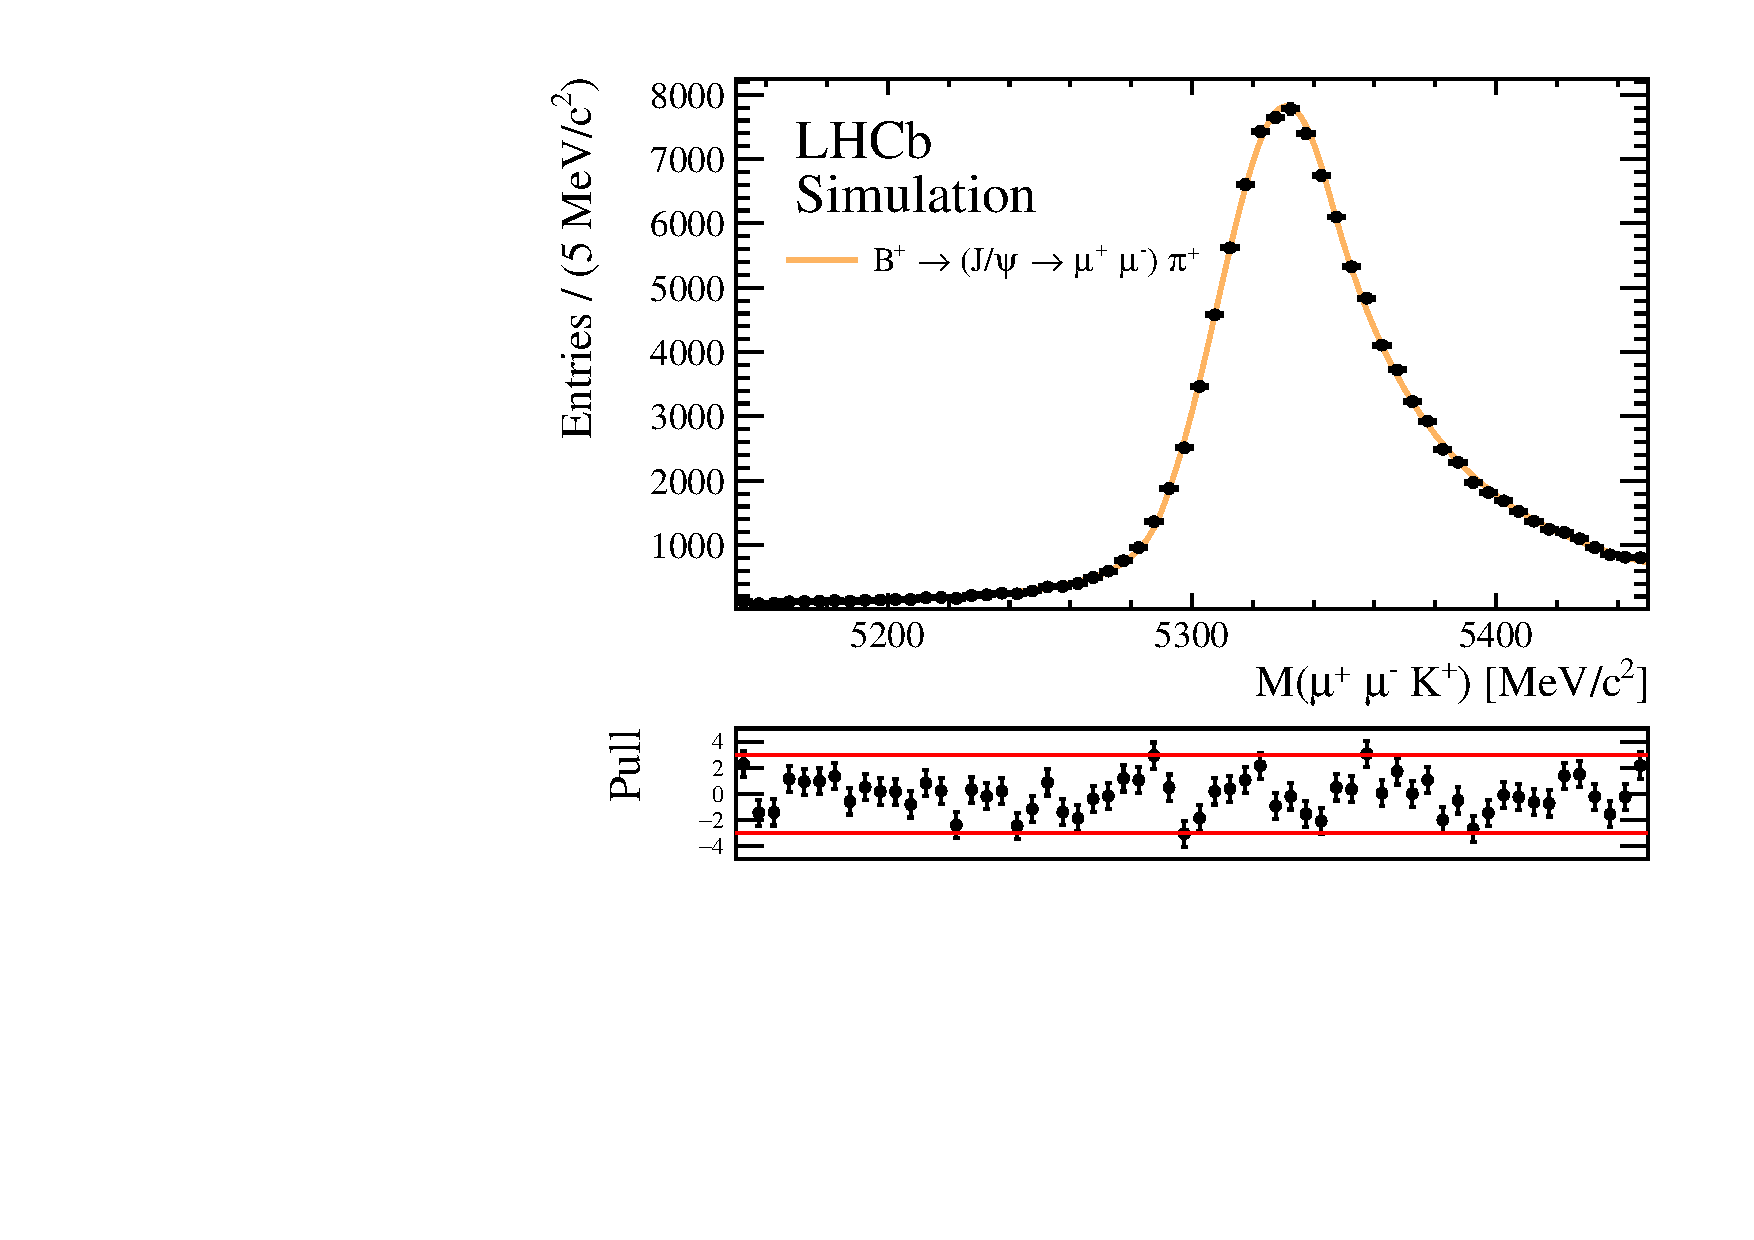
\includegraphics[width=0.45\linewidth]{./efficiency/controlchannelfits/controlpimumumcnofcmeRun1nolog.pdf}\put(-50,57){(c)}%
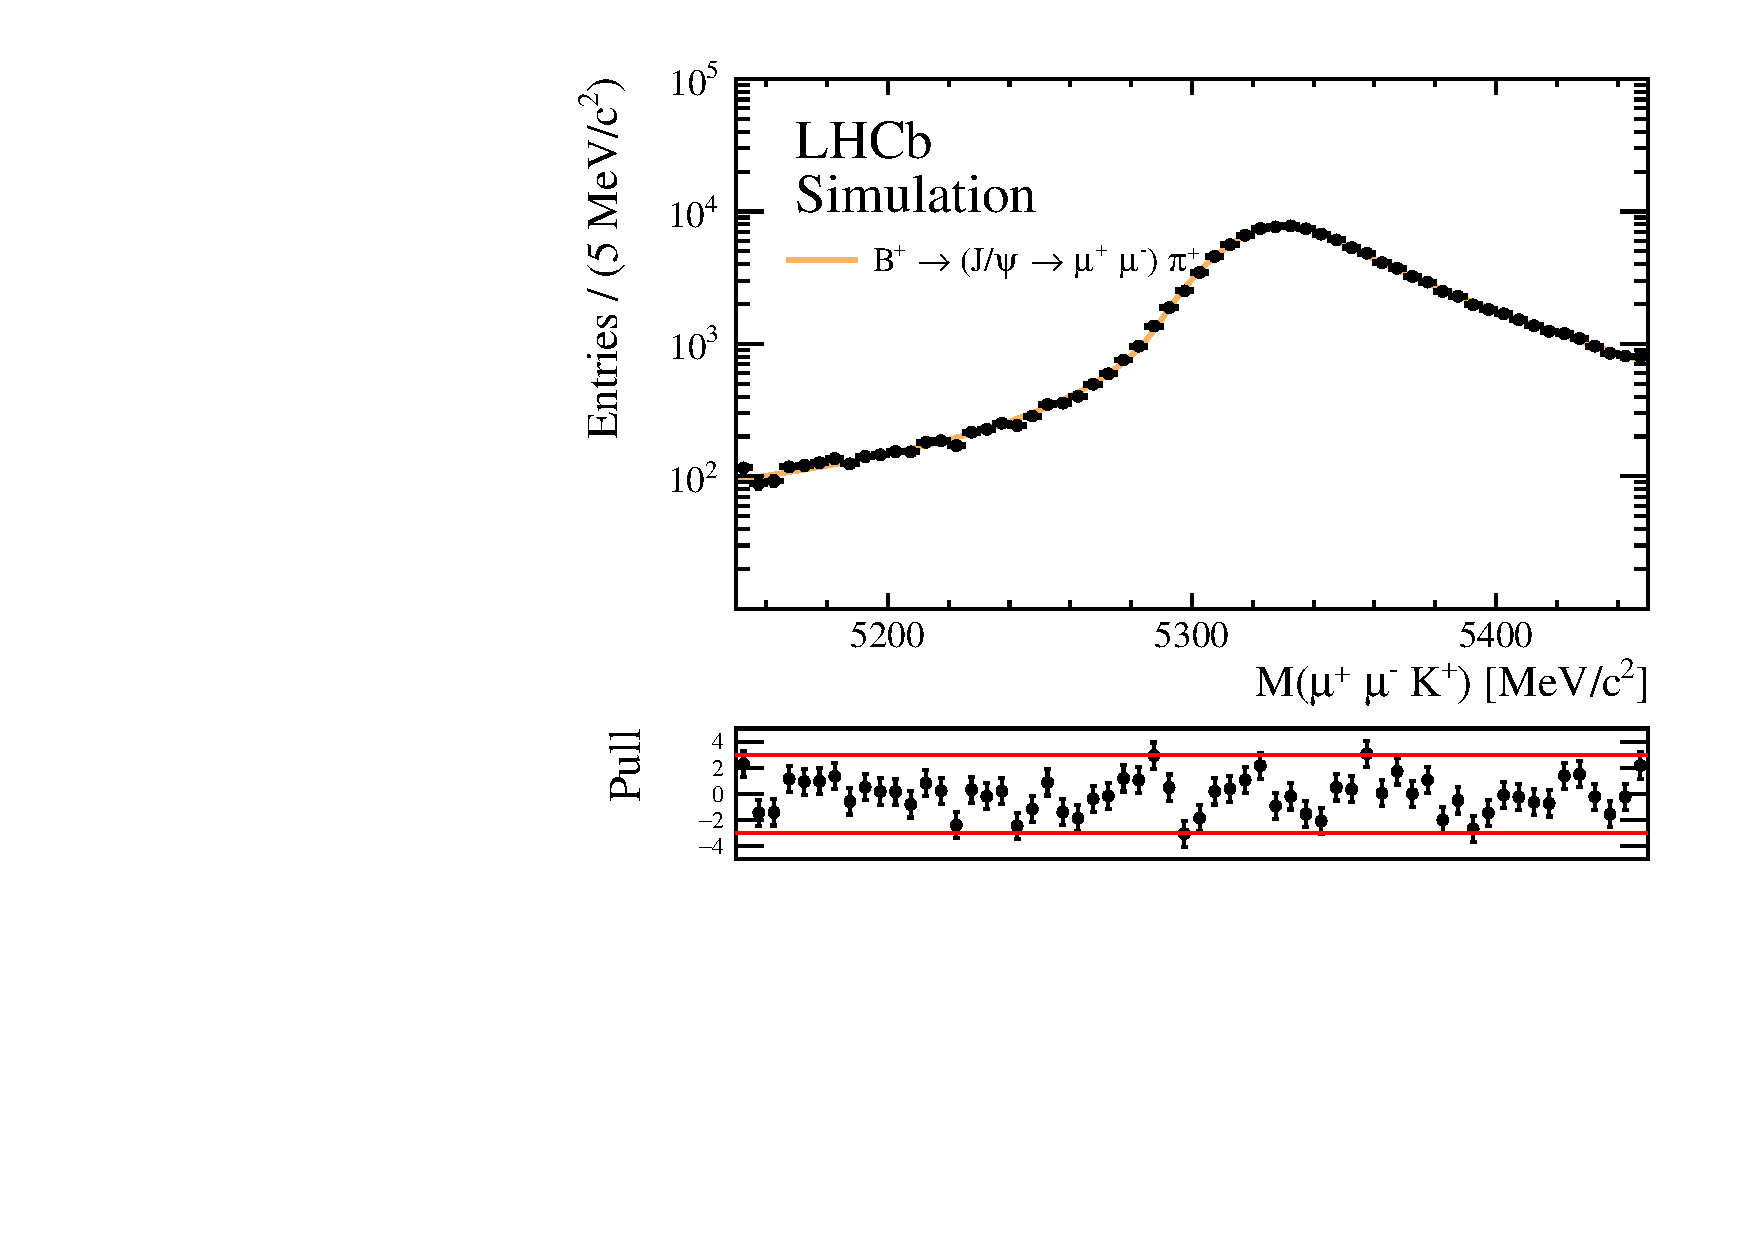
\includegraphics[width=0.45\linewidth]{./efficiency/controlchannelfits/controlpimumumcnofcmeRun1log.pdf}\put(-50,57){(d)}
	
\caption{Fit to 2012 (a) \bjpsimumuk simulation and (c) \bjpsimumupi simulation under the kaon mass hypothesis. On right, the same
 plots but with logarithmic scale instead.}
\label{fig:FitToPiMuMu}
\end{figure}

\subsubsection{Combinatorial Background}

Lastly, combinatorial background is modelled by an exponential function, where the exponential constant is let free.% The full fit model, containing description of the individual components as well as their constraints that are propagated to the extended maximum likelihood fit is given in~\autoref{tab:floatingparsummarynorm}. 


%\begin{table}[h]
%\centering
%\begin{tabular}{ l  l }
%\toprule
%Fit Parameter & Status  \\ \midrule
%\multicolumn{2}{c}{Yields} \\ \midrule
%N$_{\bjpsimumuk}$ (Signal)  &  free \\
%N$_{\bjpsimumupi}$ & free\\
%N$_{Combinatorial}$ & free\\
%\midrule
%	\multicolumn{2}{c}{Signal Shape Parameters (double-sided Ipatia)} \\
%\midrule
%	$\mu^{IP}_{\bjpsimumuk}$ & constrained from signal MC\\
%	$\sigma^{IP}_{\bjpsimumuk}$ & constrained from signal MC\\
%Others & fixed from MC\\
%\midrule
%     \multicolumn{2}{c}{\bjpsimumupi Shape Parameters (double-sided Crystal Ball)} \\
%\midrule
%	$\mu^{CB}_{\bjpsimumupi}$ & constrained from signal MC\\
%	$\sigma^{CB}_{\bjpsimumupi}$ & constrained from signal MC\\
%Others & fixed from MC \\
%\midrule
%	\multicolumn{2}{c}{Combinatorial Shape Parameters}  \\
%\midrule
%exponential par.  & free\\
%\bottomrule
%\end{tabular}
%\caption{Summary of the fit parameters and individual component constraints for the fit to \bjpsimumuk decays.}
%\label{tab:floatingparsummarynorm}
%\end{table}
%

\subsection{Normalisation Fit}
\label{normfit}
The full fit model for the normalisation data fit containing the description of the individual components as well as their constraints is given in~\autoref{tab:floatingparsummarynorm}. 


\begin{table}[h]
\centering
\begin{tabular}{ l  l }
\toprule
Fit Parameter & Status  \\ \midrule
\multicolumn{2}{c}{Yields} \\ \midrule
$N_{\bjpsimumuk}$ (Signal)  &  Free \\
$N_{\bjpsimumupi}$ & Free\\
$N_{Combinatorial}$ & Free\\
\midrule
	\multicolumn{2}{c}{Signal Shape Parameters (double-sided Ipatia)} \\
\midrule
	$\mu^{IP}_{\bjpsimumuk}$ & constrained from signal simulation\\
	$\sigma^{IP}_{\bjpsimumuk}$ & constrained from signal simulation\\
Others & Fixed from simulation\\
\midrule
     \multicolumn{2}{c}{\bjpsimumupi Shape Parameters (double-sided Crystal Ball)} \\
\midrule
	$\mu^{CB}_{\bjpsimumupi}$ & constrained from signal simulation\\
	$\sigma^{CB}_{\bjpsimumupi}$ & constrained from signal simulation\\
Others & Fixed from simulation\\
\midrule
	\multicolumn{2}{c}{Combinatorial Shape Parameters}  \\
\midrule
exponential par.  & Free\\
\bottomrule
\end{tabular}
\caption{Summary of the fit parameters and individual component constraints for the fit to the \bjpsimumuk decays.}
\label{tab:floatingparsummarynorm}
\end{table}

The $B^{+} \rightarrow (J/\psi \rightarrow \mu^{+} \mu^{-}) K^{+}$ signal yield is extracted by performing an unbinned extended maximum likelihood fit with the full fit model to the invariant $\mu^{+} \mu^{-} K^{+}$ distribution in $5150\mevcc<M_{B^{+}}<5450\mevcc$. Fits to the $ B^{+} \rightarrow (J/\psi \rightarrow \mu^{+} \mu^{-}) K^{+}$ for Run \Rn{1} and Run \Rn{2} are shown in~\autoref{fig:run1jpsikfitnofcme}. Yields from the fit to \bjpsimumuk are obtained and summarized in~\autoref{tab:normchannelyields}.

\begin{figure}[H]
\centering
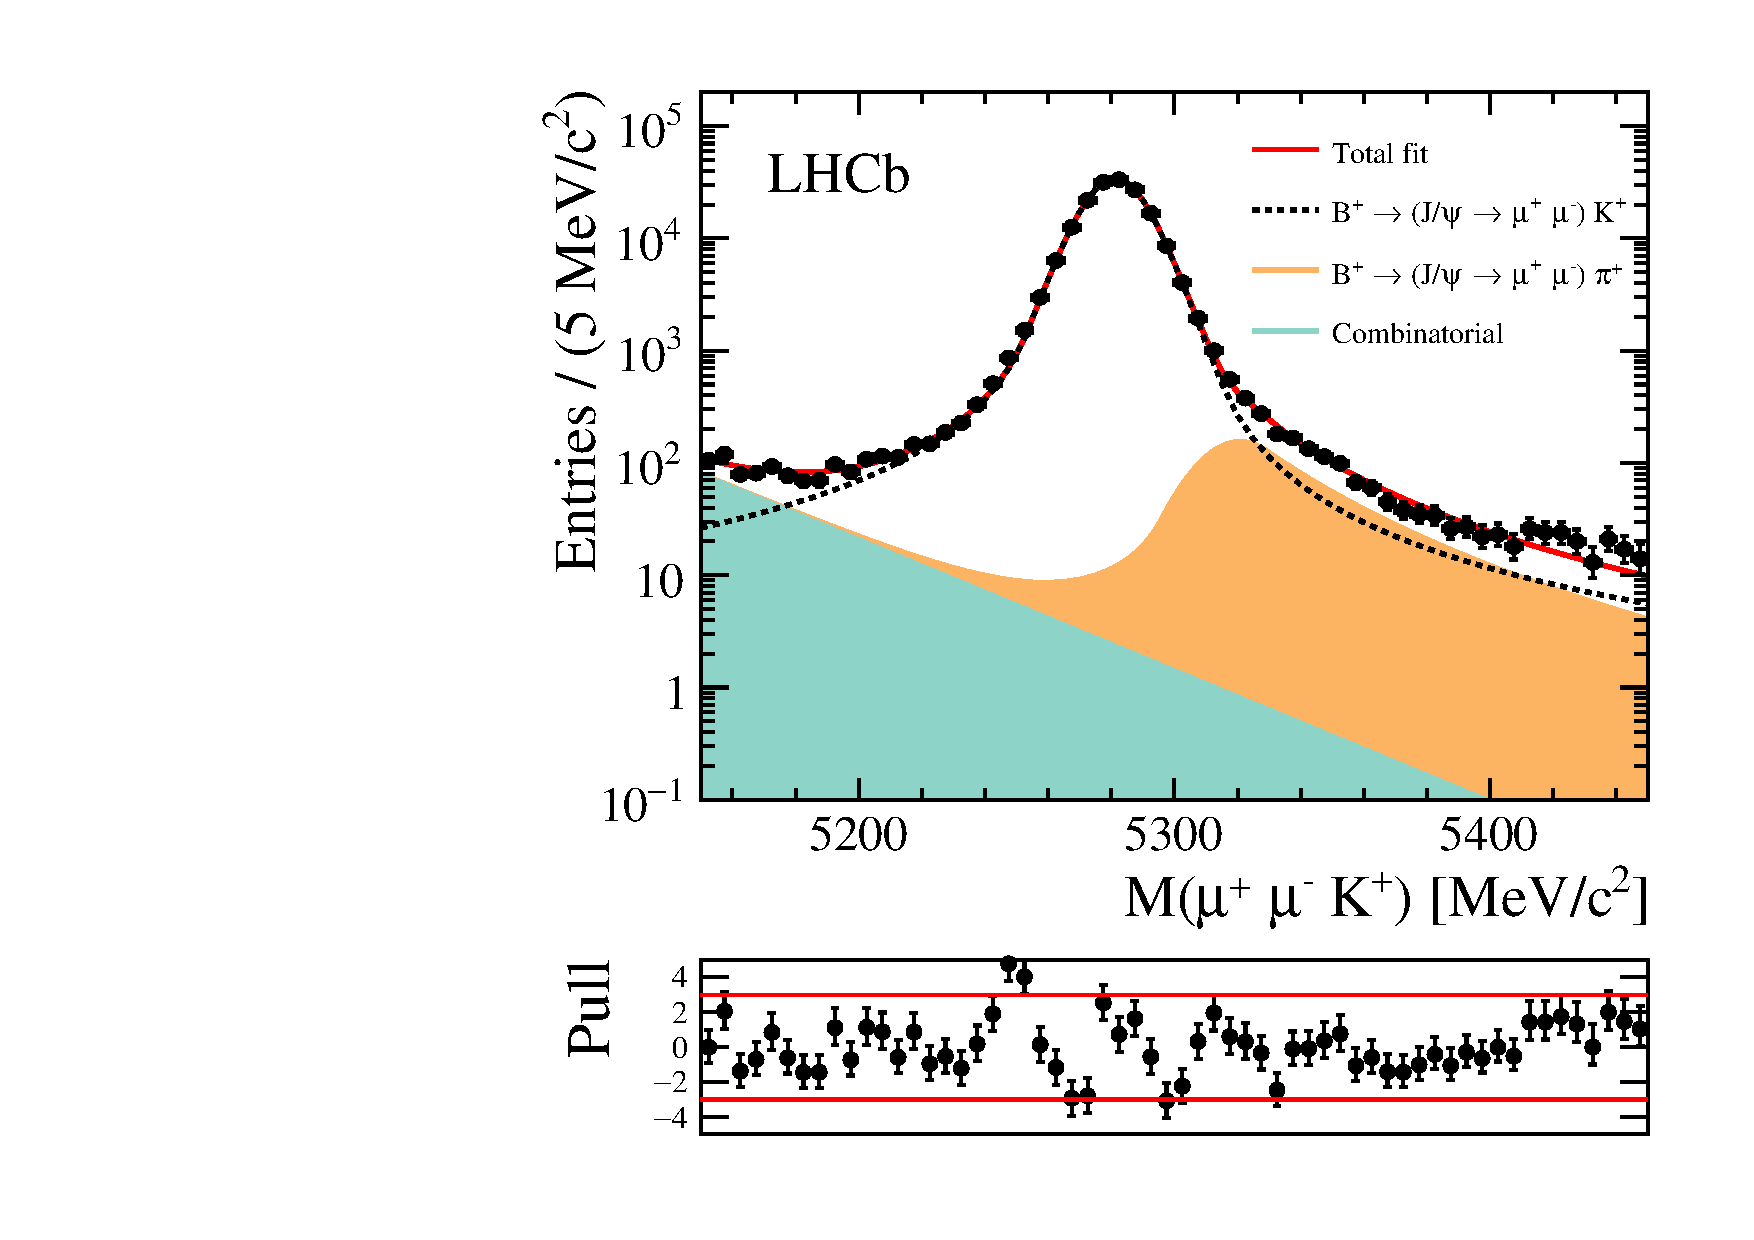
\includegraphics[width=0.5\linewidth]{./efficiency/controlchannelfits/controlnofcmeRun1.pdf}\put(-50,133){(a)}%
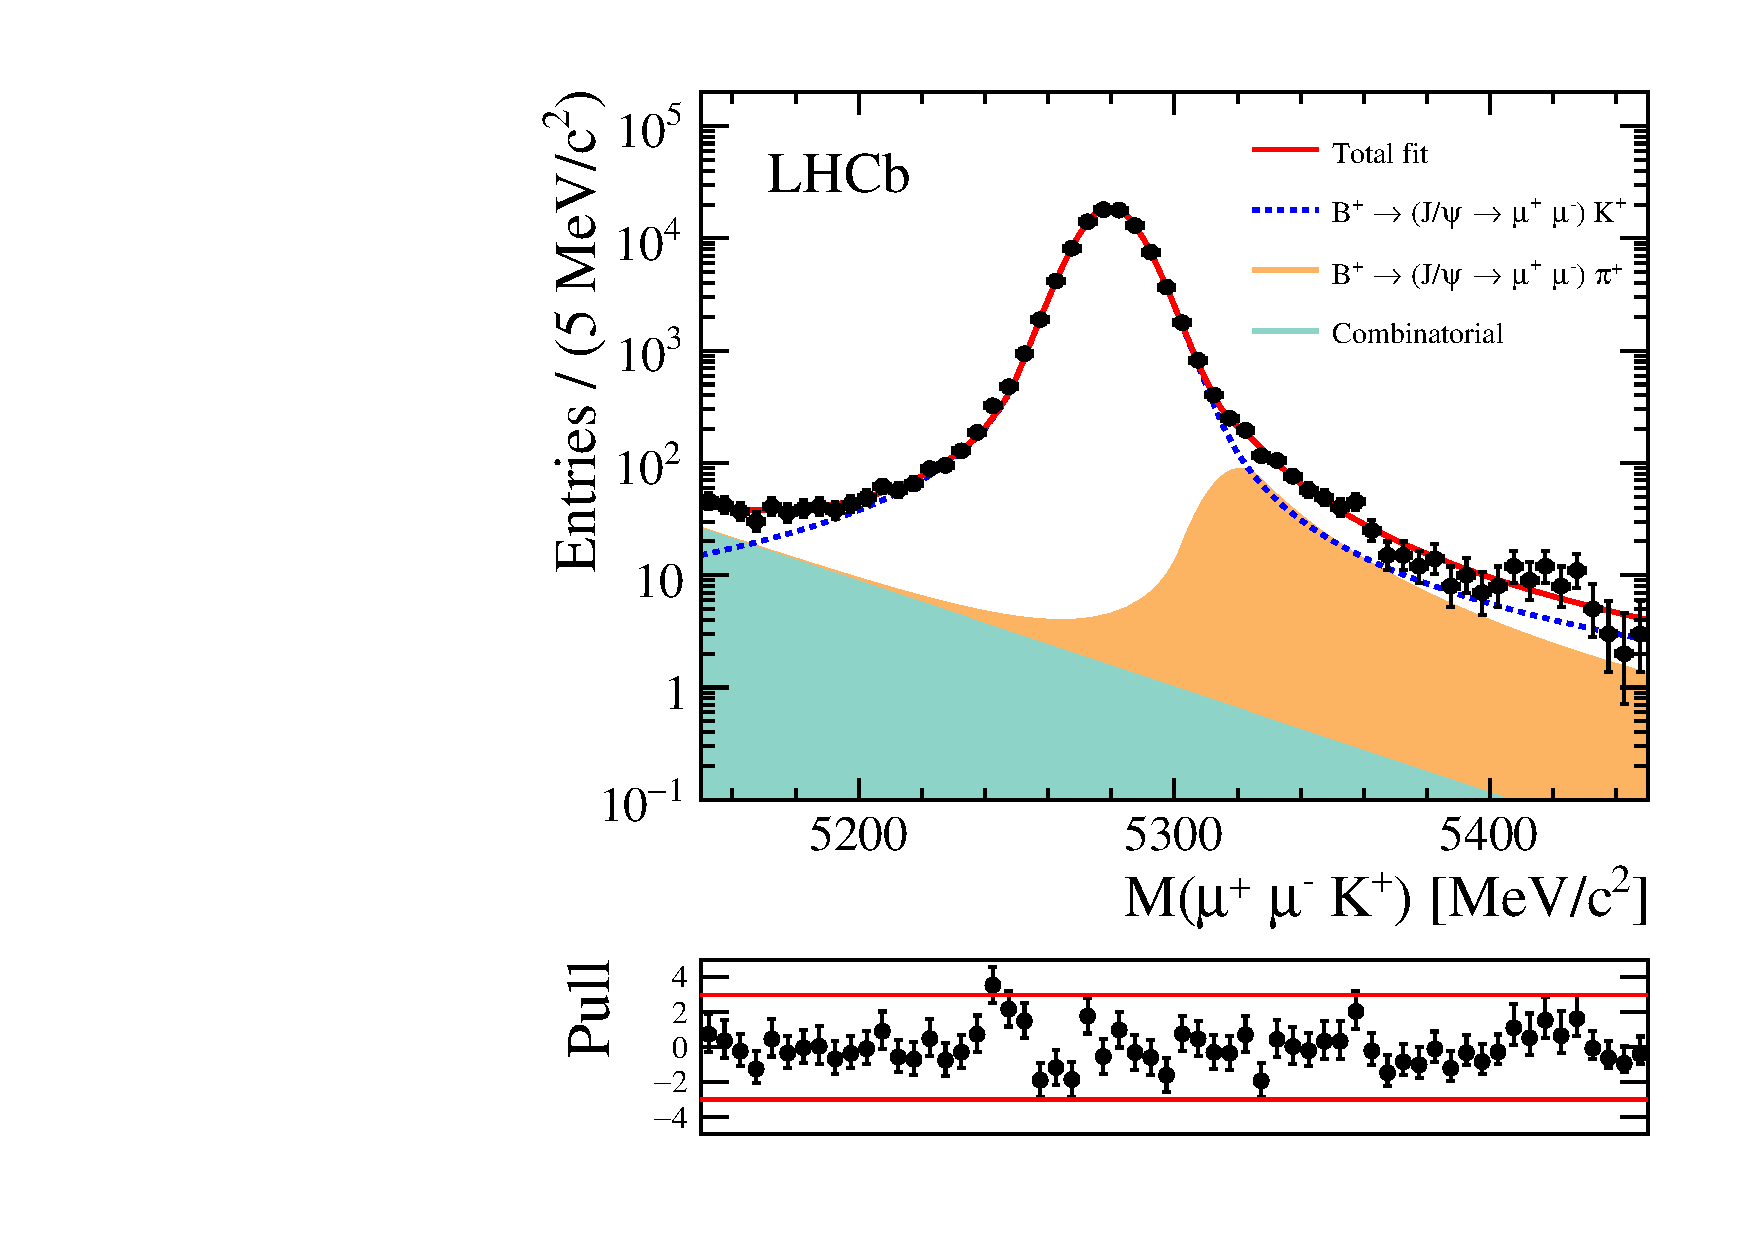
\includegraphics[width=0.5\linewidth]{./efficiency/controlchannelfits/controlnofcme2016.pdf}\put(-50,133){(b)}
\newline
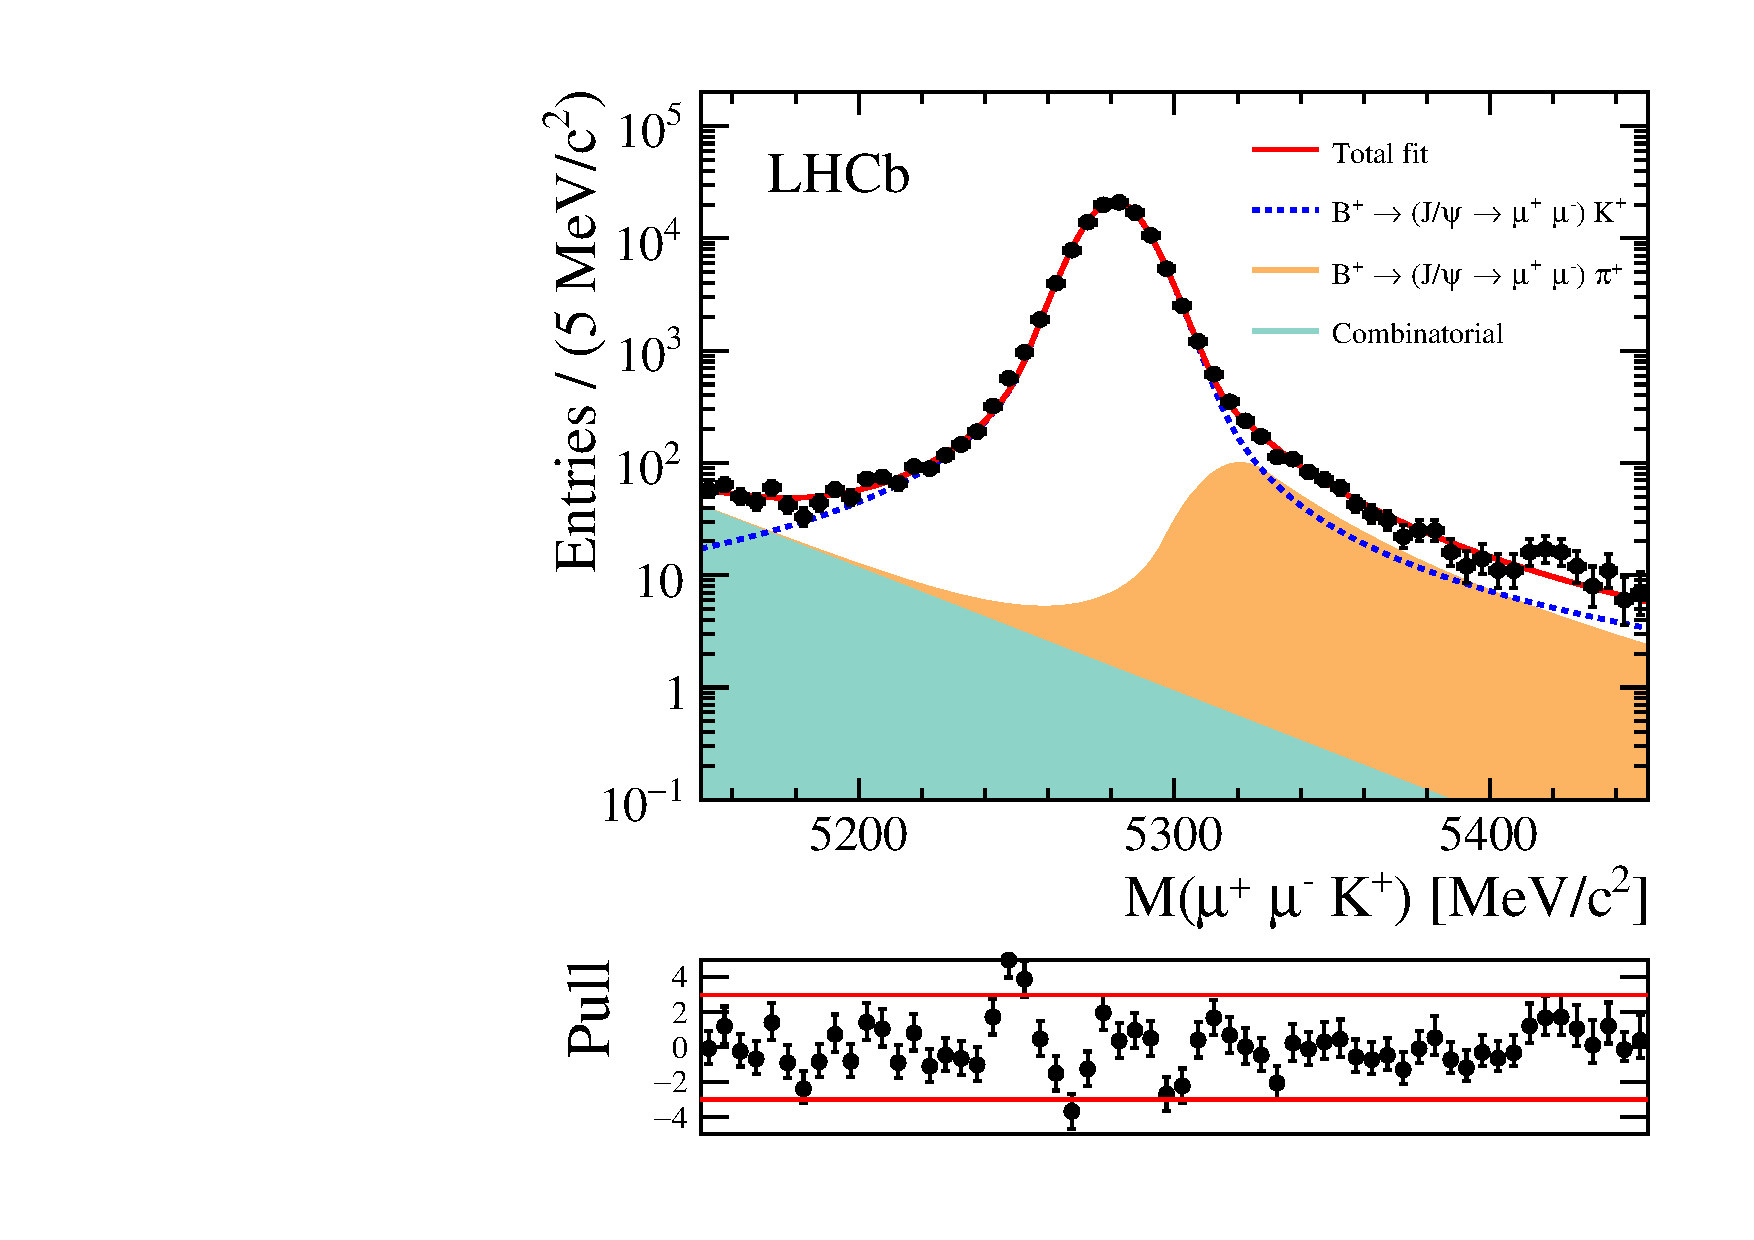
\includegraphics[width=0.5\linewidth]{./efficiency/controlchannelfits/controllowhfcmeRun1.pdf}\put(-50,133){(c)}%
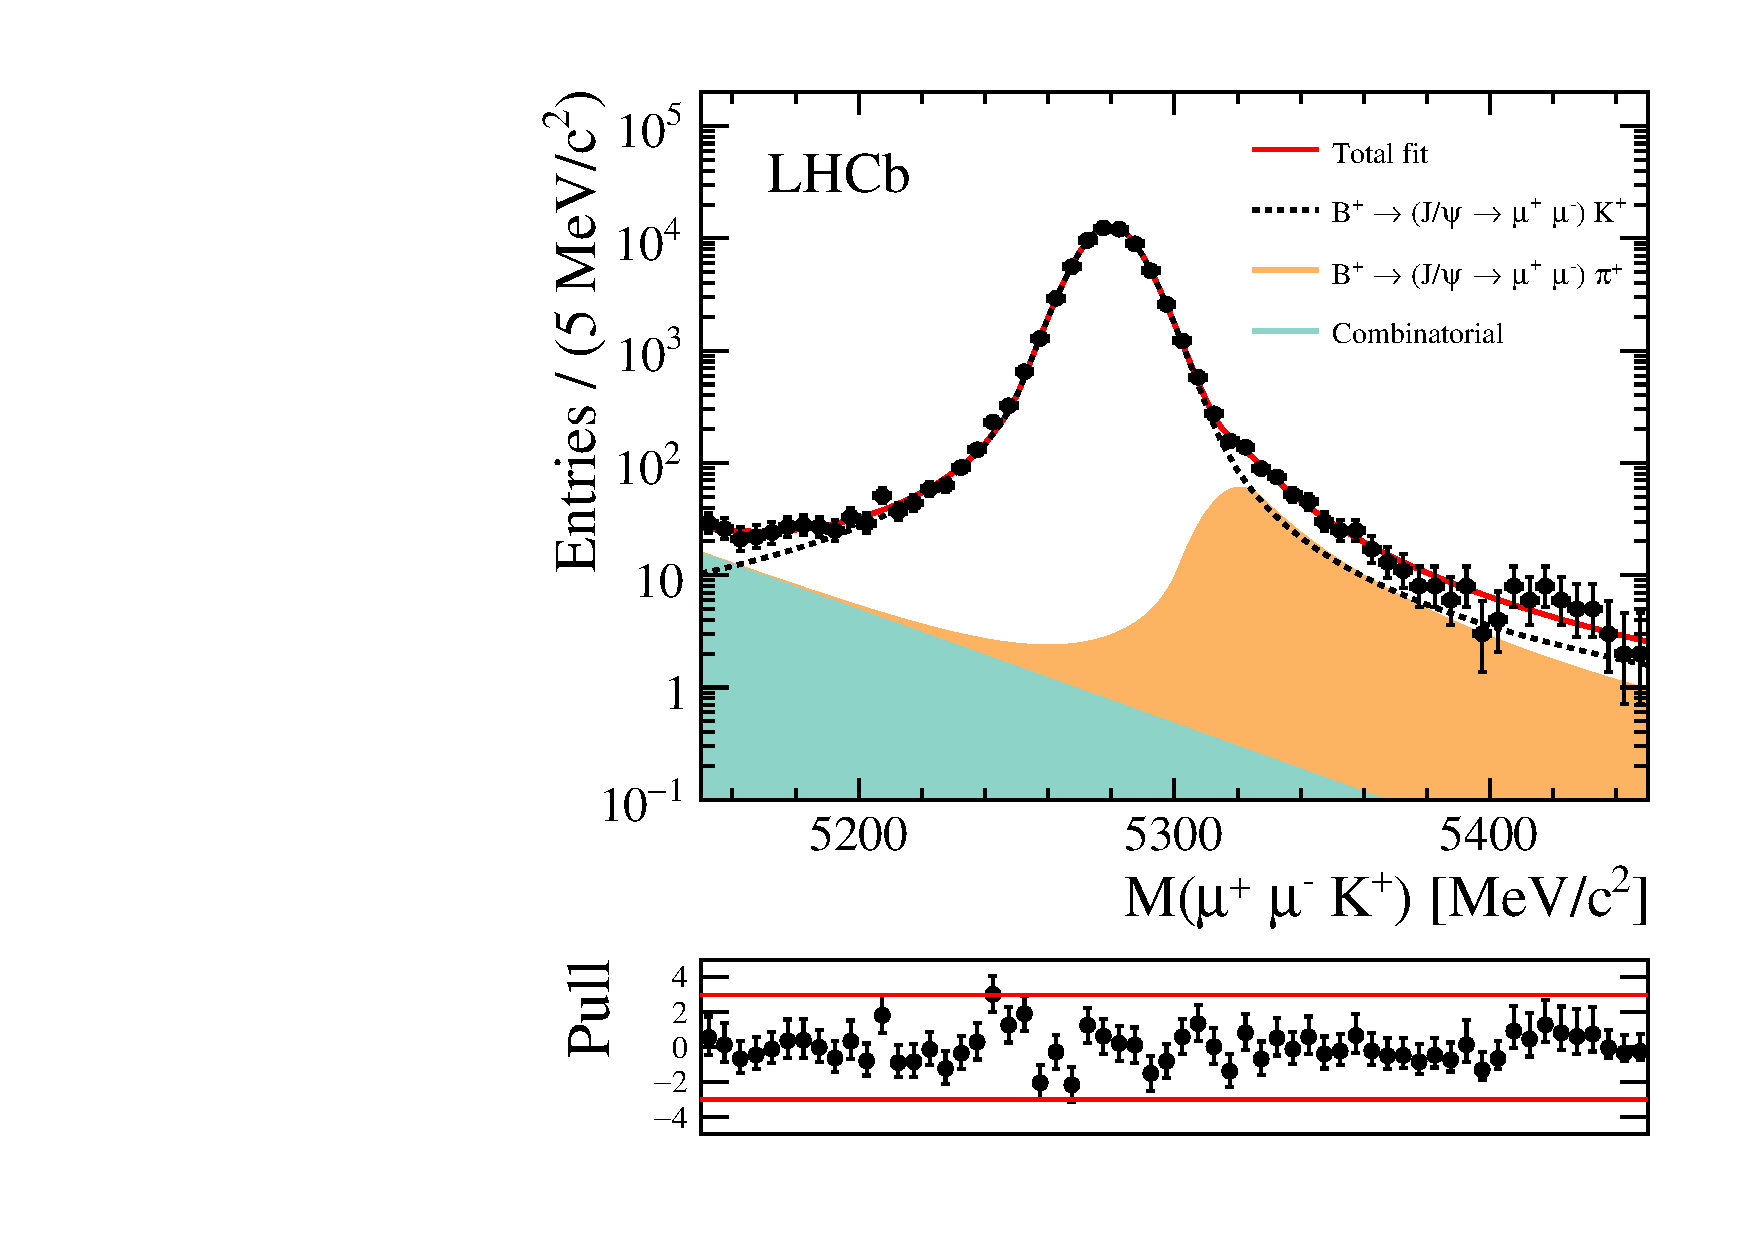
\includegraphics[width=0.5\linewidth]{./efficiency/controlchannelfits/controllowfcme2016.pdf}\put(-50,133){(d)}
\newline
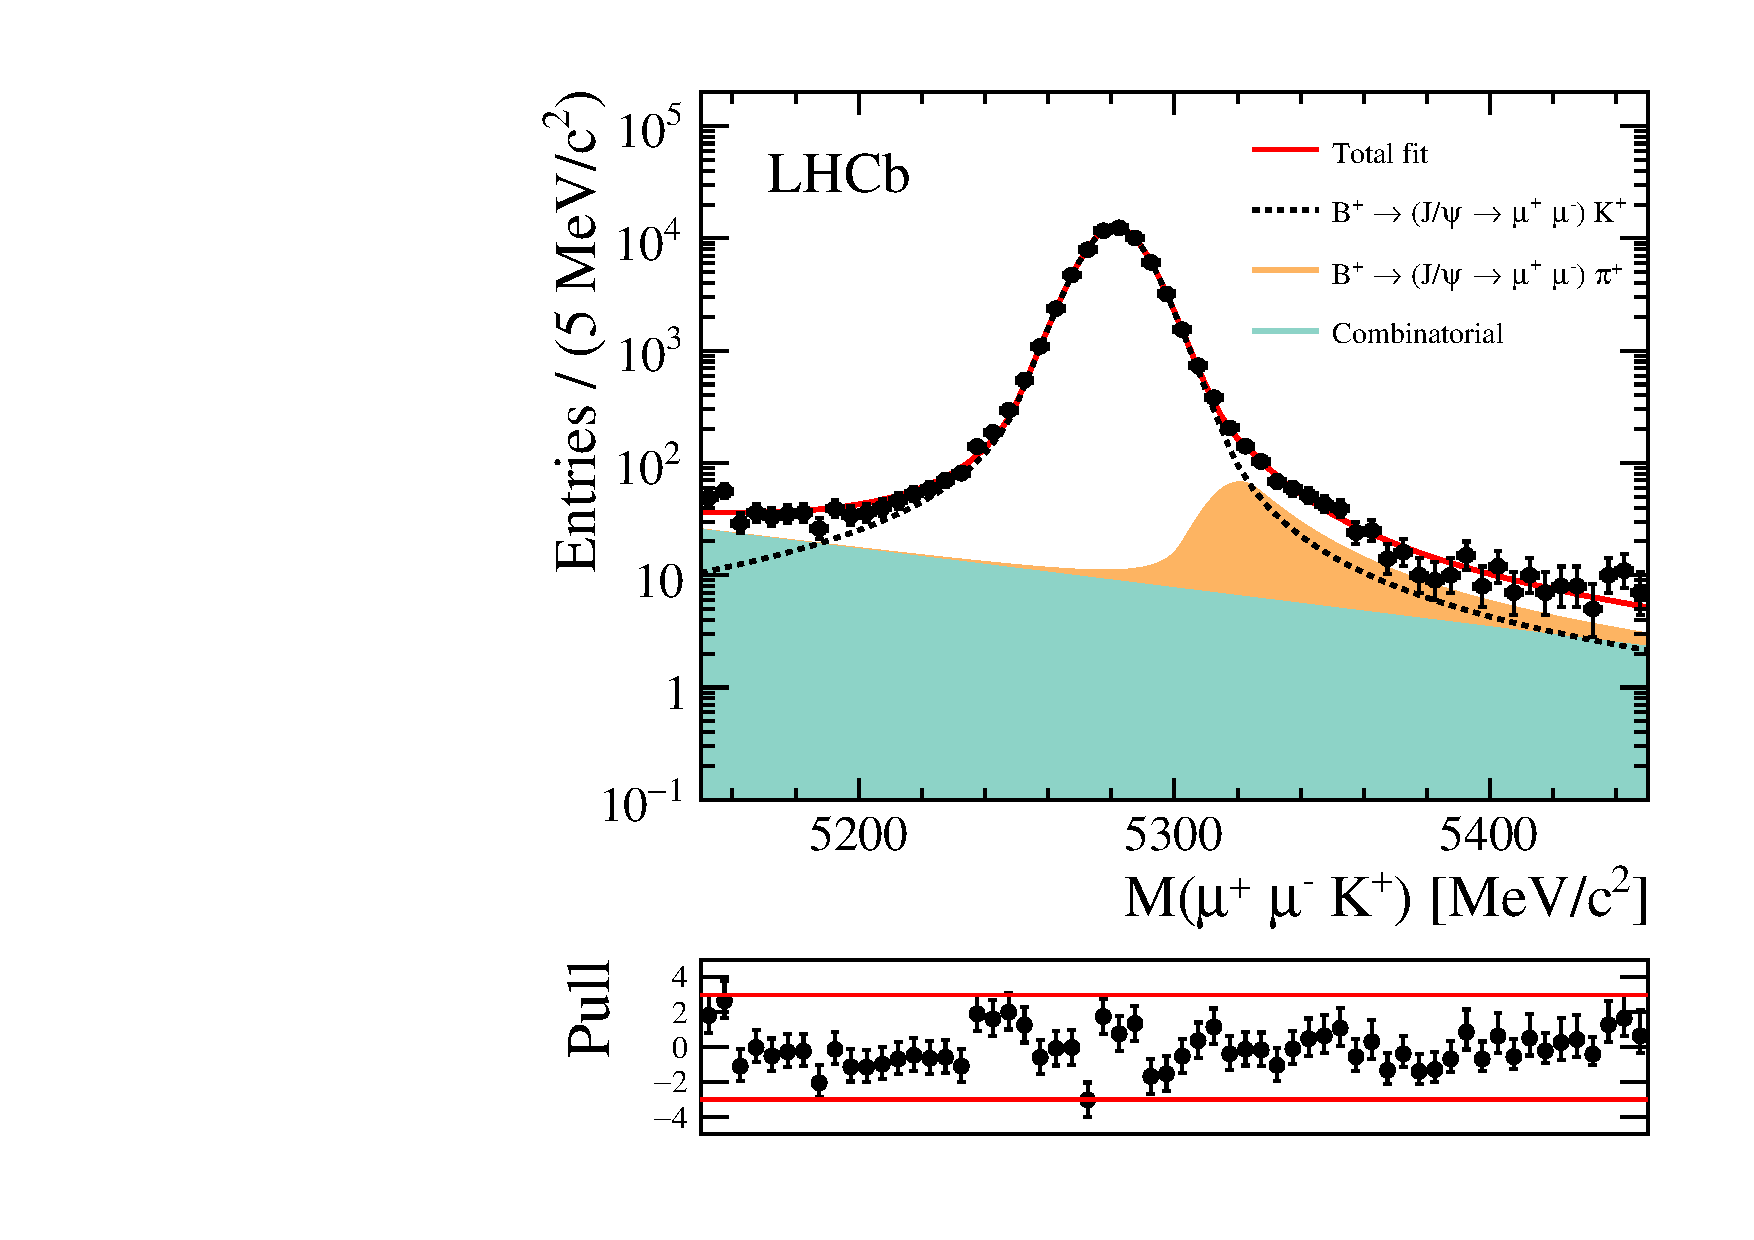
\includegraphics[width=0.5\linewidth]{./efficiency/controlchannelfits/controlhighfcmeRun1.pdf}\put(-50,133){(e)}%
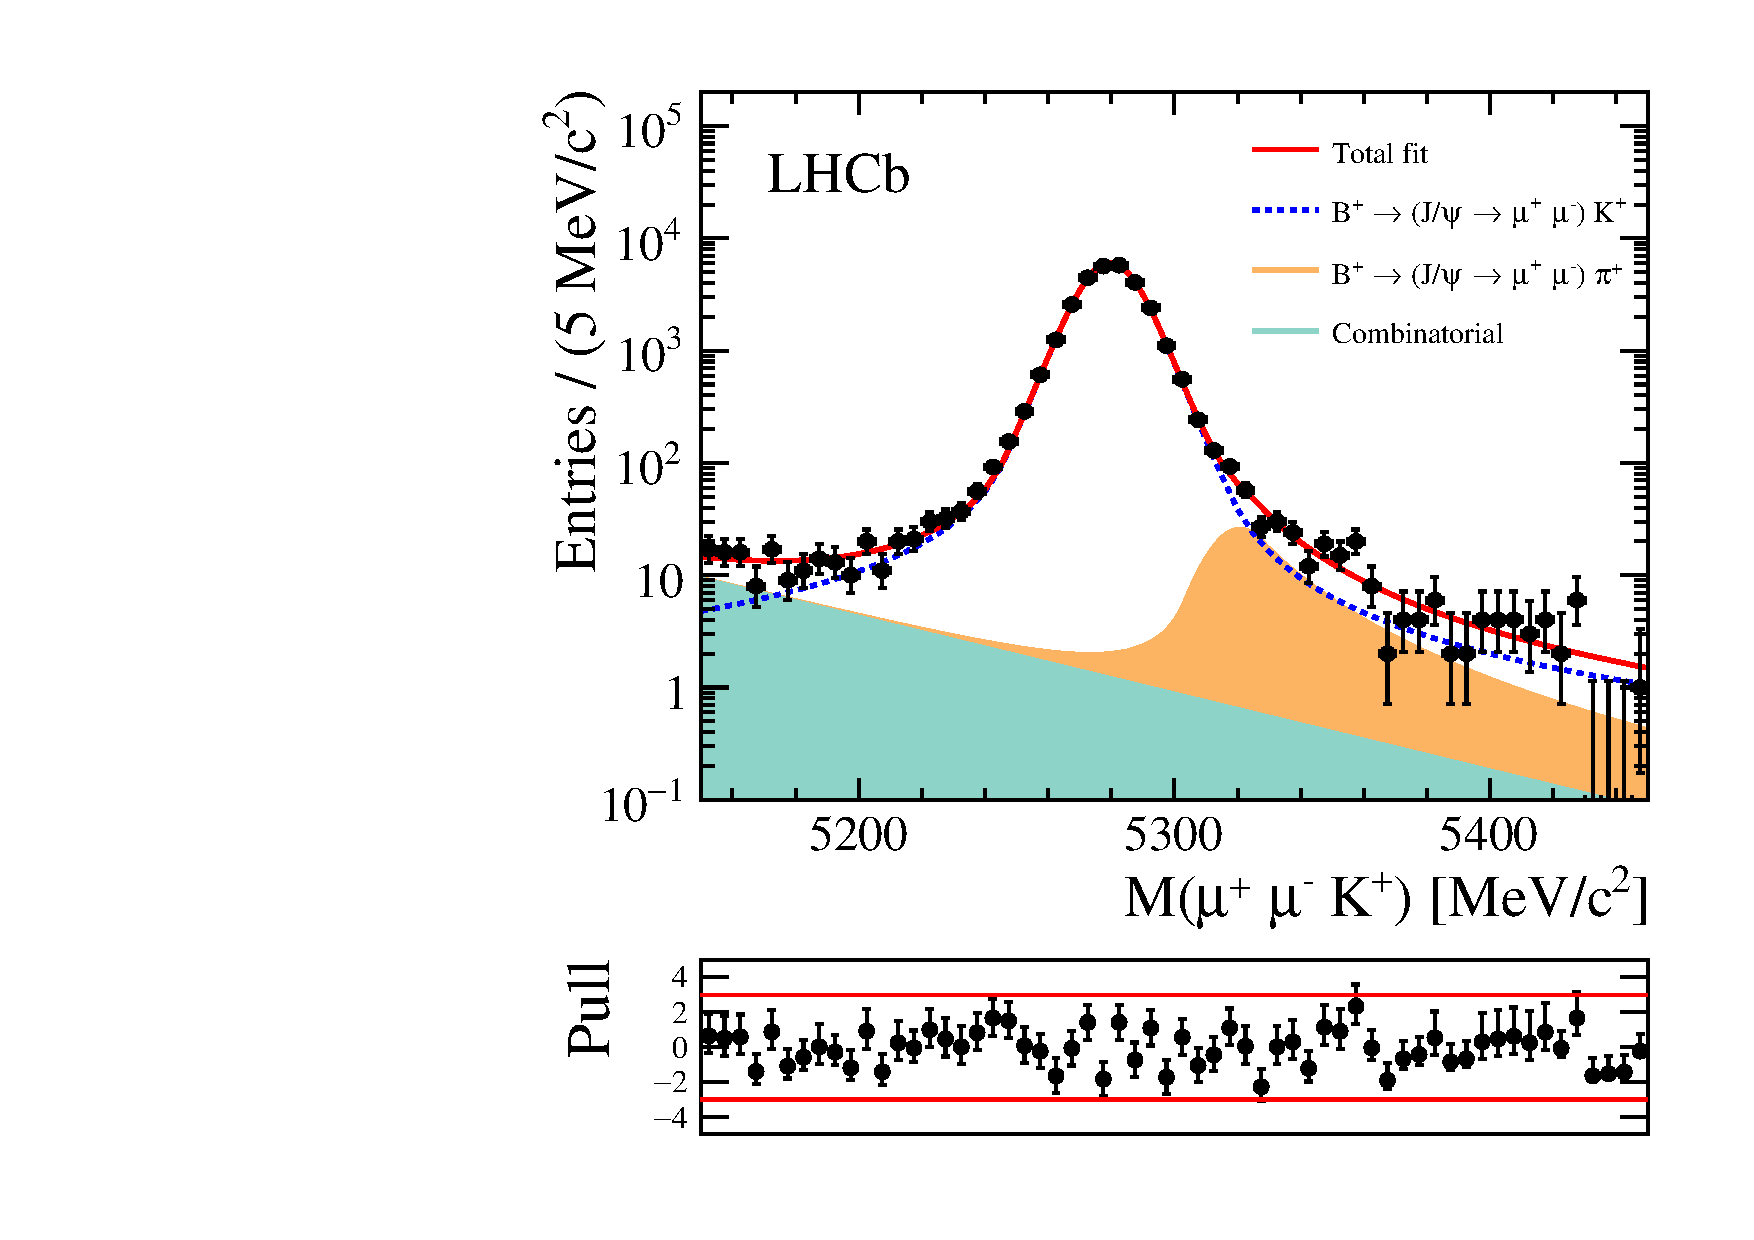
\includegraphics[width=0.5\linewidth]{./efficiency/controlchannelfits/controlhighfcme2016.pdf}\put(-50,133){(f)}
\caption{Fit results in logarithmic scale to (a) Run \Rn{1} (b) Run \Rn{2} $\mu^{+} \mu^{-} K^{+}$ mass spectrum with no fractional corrected mass split, (c)(d) low FCME bin, (e)(f)high FCME bin.}
\label{fig:run1jpsikfitnofcme}
\end{figure}




\begin{table}[H]
\begin{center}
\begin{tabular}{ l  l  l  l }
\toprule
Sample & Stripping & Split  &Yields \\
\midrule
	$N_{B^{+} \rightarrow J/\psi K^{+}}$  & Run \Rn{1} & $\sigma_{\mathrm{NOFCME}}$ & 173422$\pm$446  \\
	$N_{B^{+} \rightarrow J/\psi K^{+}}$  & Run \Rn{2} & $\sigma_{\mathrm{NOFCME}}$ &94491$\pm$313  \\
\midrule
	$N_{B^{+} \rightarrow J/\psi K^{+}}$  & Run \Rn{1} & $\sigma_{\mathrm{lowFCME}}$ & 109224$\pm$337  \\
	$N_{B^{+} \rightarrow J/\psi K^{+}}$  & Run \Rn{2} & $\sigma_{\mathrm{lowFCME}}$ & 64723$\pm$259  \\
\midrule
	$N_{B^{+} \rightarrow J/\psi K^{+}}$  & Run \Rn{1} & $\sigma_{\mathrm{highFCME}}$ &64078$\pm$257  \\
	$N_{B^{+} \rightarrow J/\psi K^{+}}$  & Run \Rn{2} & $\sigma_{\mathrm{highFCME}}$ & 29760$\pm$176  \\
\bottomrule
\end{tabular}
\end{center}
	\caption{ \bjpsimumuk signal yield obtained from fits to $\mu^{+} \mu^{-} K^{+}$ mass spectrum shown in~\autoref{fig:run1jpsikfitnofcme}.}
\label{tab:normchannelyields}
\end{table}

\subsection{Signal Channel Parametrisation}
\label{sigpara}
To fit the signal data, the default fitting strategy is to use a simultaneous unbinned maximum likelihood fit to the $\mu^{+} \mu^{-} \mu^{+}$ corrected mass spectrum to combined Run \Rn{1} and \Rn{2} dataset after the full selection in two bins of fractional corrected mass error, which is denoted as the simultaneous fit. As a cross-check a non-simultaneous fit, where no splitting in bins of corrected mass is done, is denoted as non-simultaneous fit. The parametrisation of all the components for the full signal model fit is described below.


\subsubsection{Signal}
The full fit to Run \Rn{1} and Run \Rn{2} data requires the signal shape knowledge for the combined dataset. This is obtained from a Run \Rn{1} and Run \Rn{2} signal simulation \textit{cocktail}. The cocktail is created after full selection by assigning event-by-event weights, \textit{$w^{i}$}, which capture the differences between Run \Rn{1} and Run \Rn{2} simulation, that ware not considered by the full selection.

Firstly, weights that reflect the expected difference due to increased luminosity are computed. To obtain these signal weights, the following conditions must be satisfied

%Signal shape for Run \Rn{1} and Run \Rn{2} is described by probability density function (P.D.F) in corrected mass taken from $B^{+} \rightarrow \mu^{+} \mu^{-} \mu^{+} \nu_\mu$ 2012 MC and 2016 MC cocktail. After all respective
%selection, this cocktail is created by assigning event-by-event weights. Signal event-by-event weights, \textit{$w^{i}$}, to create cocktail come from differences between 2012 MC and 2016 MC. To obtain signal weights, following conditions must be satisfied,
\begin{equation}
n^{2012}=\mathcal{L}^{2012} \times \sigma^{2012}_{pp \rightarrow b \overline{b}},
\end{equation}

\begin{equation}
n^{2016}=\mathcal{L}^{2016} \times \sigma^{2016}_{pp \rightarrow b \overline{b}},
\end{equation}

\begin{equation}
w^{2012} \times N^{2012} + w^{2016} \times N^{2016} = N^{2012} + N^{2016},
\end{equation}

\begin{equation}
\frac{w^{2012} \times N^{2012}}{w^{2016} \times N^{2016}} = \frac{n^{2012}}{n^{2016}}.
\end{equation}

These constraints yield the following value for event-by-event (or rather yearly) weights


\begin{equation}
w^{2012}= \frac{N^{2012}+N^{2016}}{N^{2012}\times(1.0+\frac{n^{2016}}{n^{2012}})}=0.931
\end{equation}


\begin{equation}
w^{2016}= \frac{N^{2016}+N^{2012}}{N^{2016}\times(1.0+ \frac{n^{2012}}{n^{2016}})}=1.073,
\end{equation}



where $N^{2012},N^{2016}$ number of events at \textit{generator level}, $\mathcal{L}^{2012},\mathcal{L}^{2016}$ are integrated luminosities, and $\sigma^{2012}_{pp \rightarrow b \overline{b}}, \sigma^{2016}_{pp \rightarrow b \overline{b}}$ are cross-sections in a given year. $N^{2012},N^{2016}$ number of events at \textit{generator level} is obtained by dividing the number of reconstructed events $N_{REC}$ by the reconstruction efficiency $\varepsilon_{REC}$ (see~\autoref{tab:effsumarry}). Values for these variables are summarized in ~\autoref{tab:MCweightNOFCME}.


\begin{table}[h]
\centering
\begin{tabular}{ l  c  c }
\toprule
Summary & 2012 Simulation & 2016 Simulation \\
\midrule
%$\epsilon_{PID}$ & taken from PID & taken from PID  \\
%$\epsilon_{GEN}$  & 0.18643$\pm$0.00029 & 0.1977$\pm$0.0004 \\


$N_{REC}$  & 1114130 & 1107715 \\
$\mathcal{L}$ & 2968 $\rm{pb^{-1}}$ & 1612 $\rm{pb^{-1}}$ \\
$\sigma_{pp \rightarrow b \overline{b}}$ & 1 & 2  \\
\bottomrule
\end{tabular}
	\caption{Signal simulation weights used to create cocktail of mixed Run \Rn{1} (2012) and Run \Rn{2} (2016) cocktail. The cross-sections listed here are not absolute numbers, but rather relative as only their ratio matters.}
\label{tab:MCweightNOFCME}
\end{table}

Secondly, event-by-event weight which differs between Run \Rn{1} and \Rn{2} that need to be accounted is the PID efficiency $\varepsilon_{PID}$ (see~\autoref{tab:effsumarry}), which depends on the kinematics of the final state particles. It is denoted as $w^{i\varepsilon\{2012,2016\}}_{\varepsilon^{i}_{PID}}$. 

The final weight of an event depending on Run \Rn{1} and Run \Rn{2} is calculated 

\begin{equation}
	w^{i\varepsilon\{2012,2016\}}_{total}=  w^{i\varepsilon\{2012,2016\}} \times w^{i\varepsilon\{2012,2016\}}_{\varepsilon^{i}_{PID}}.
\end{equation}

After obtaining combined Run \Rn{1} and \Rn{2} signal \textit{cocktail}, fit to this weighted simulation is done with \textbf{the shape} in the corrected mass modelled by a double-sided Crystal Ball function~\autoref{IP}. The fit and its parameters can be seen in~\autoref{fig:MCSignalFit}. The function describing this shape is denoted as $f^{sig}$ and hence is a function of 6 parameters for the non-simultaneous fit and 12 parameters for the simultaneous fit.

\begin{figure}[H]
\centering
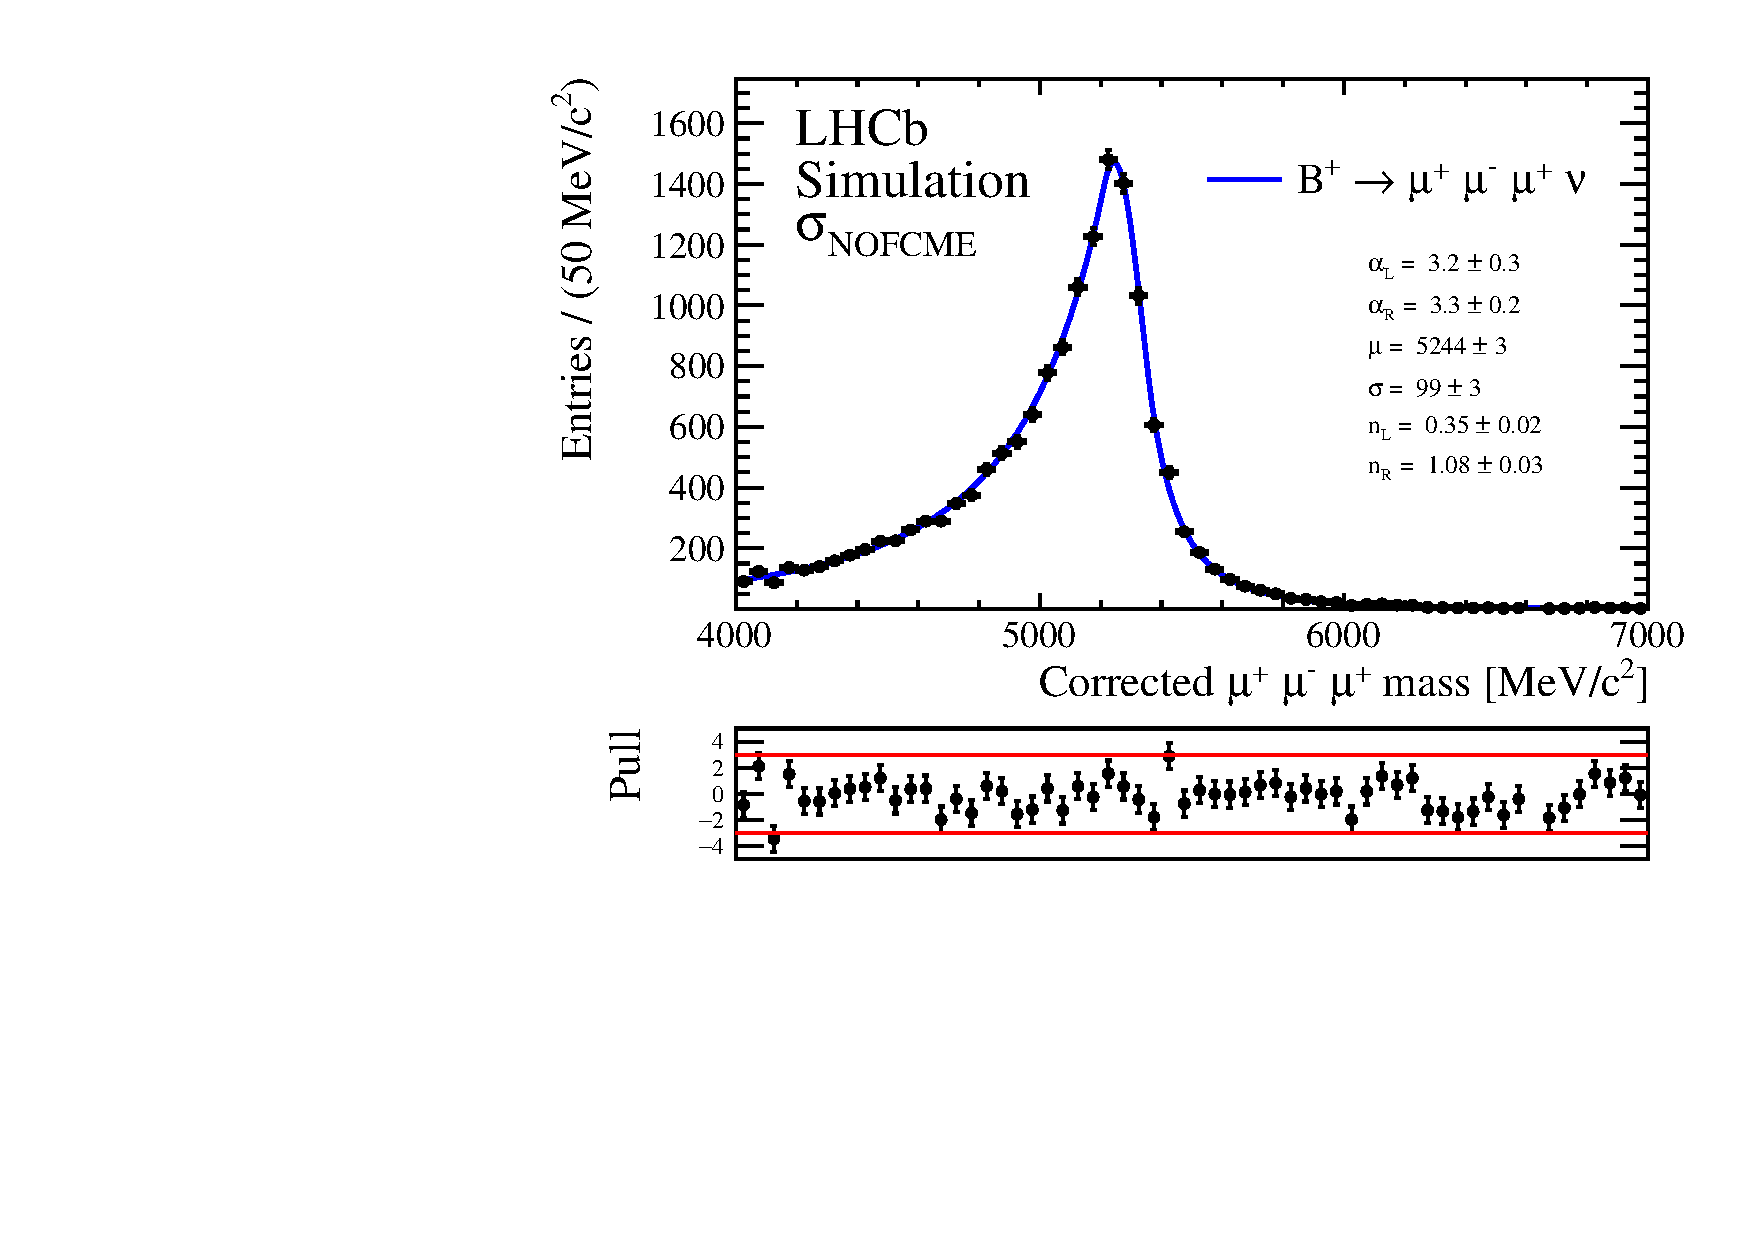
\includegraphics[width=0.5\linewidth]{./efficiency/signalfits/signalmc/sigmcnofcmeRun1nolog.pdf}\put(-30,60){(a)}
\newline
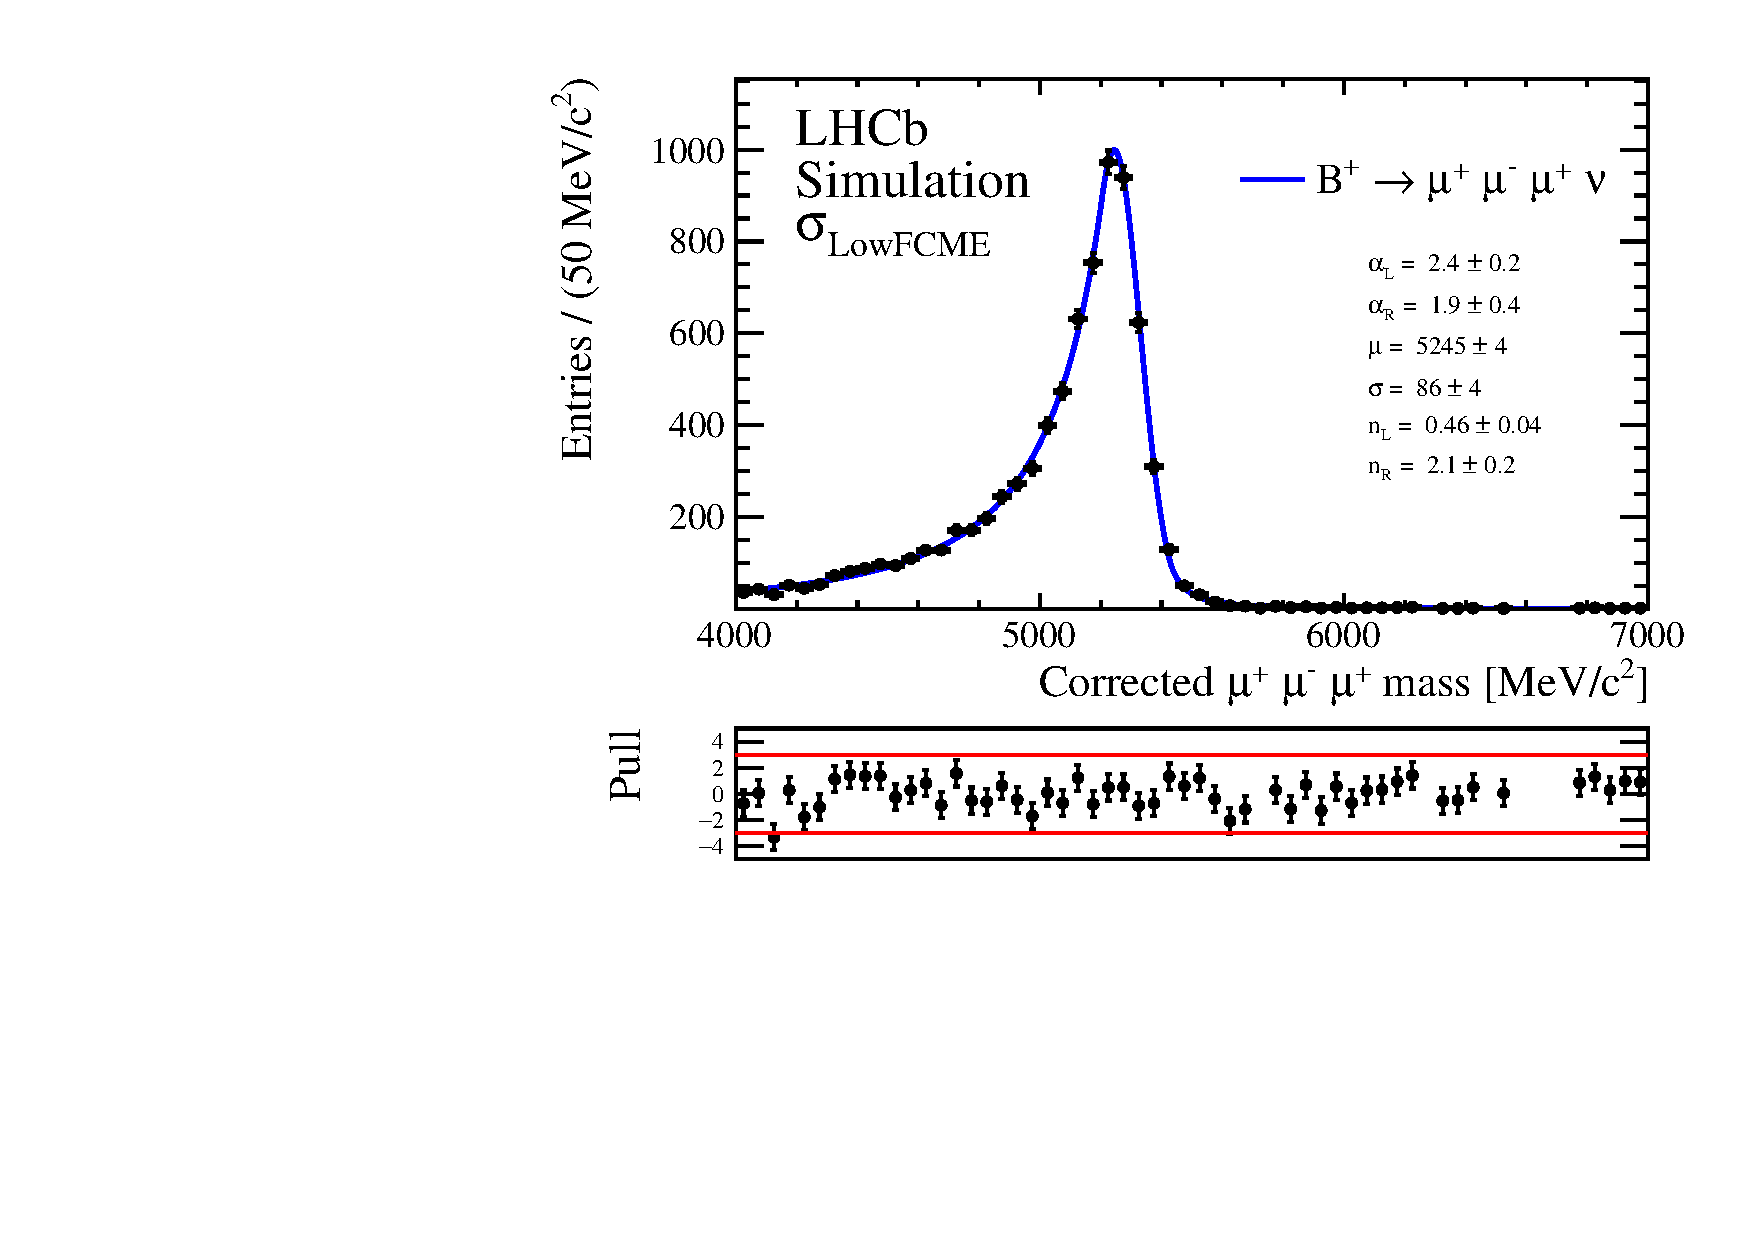
\includegraphics[width=0.5\linewidth]{./efficiency/signalfits/signalmc/sigmclowfcmeRun1nolog.pdf}\put(-30,60){(b)}%
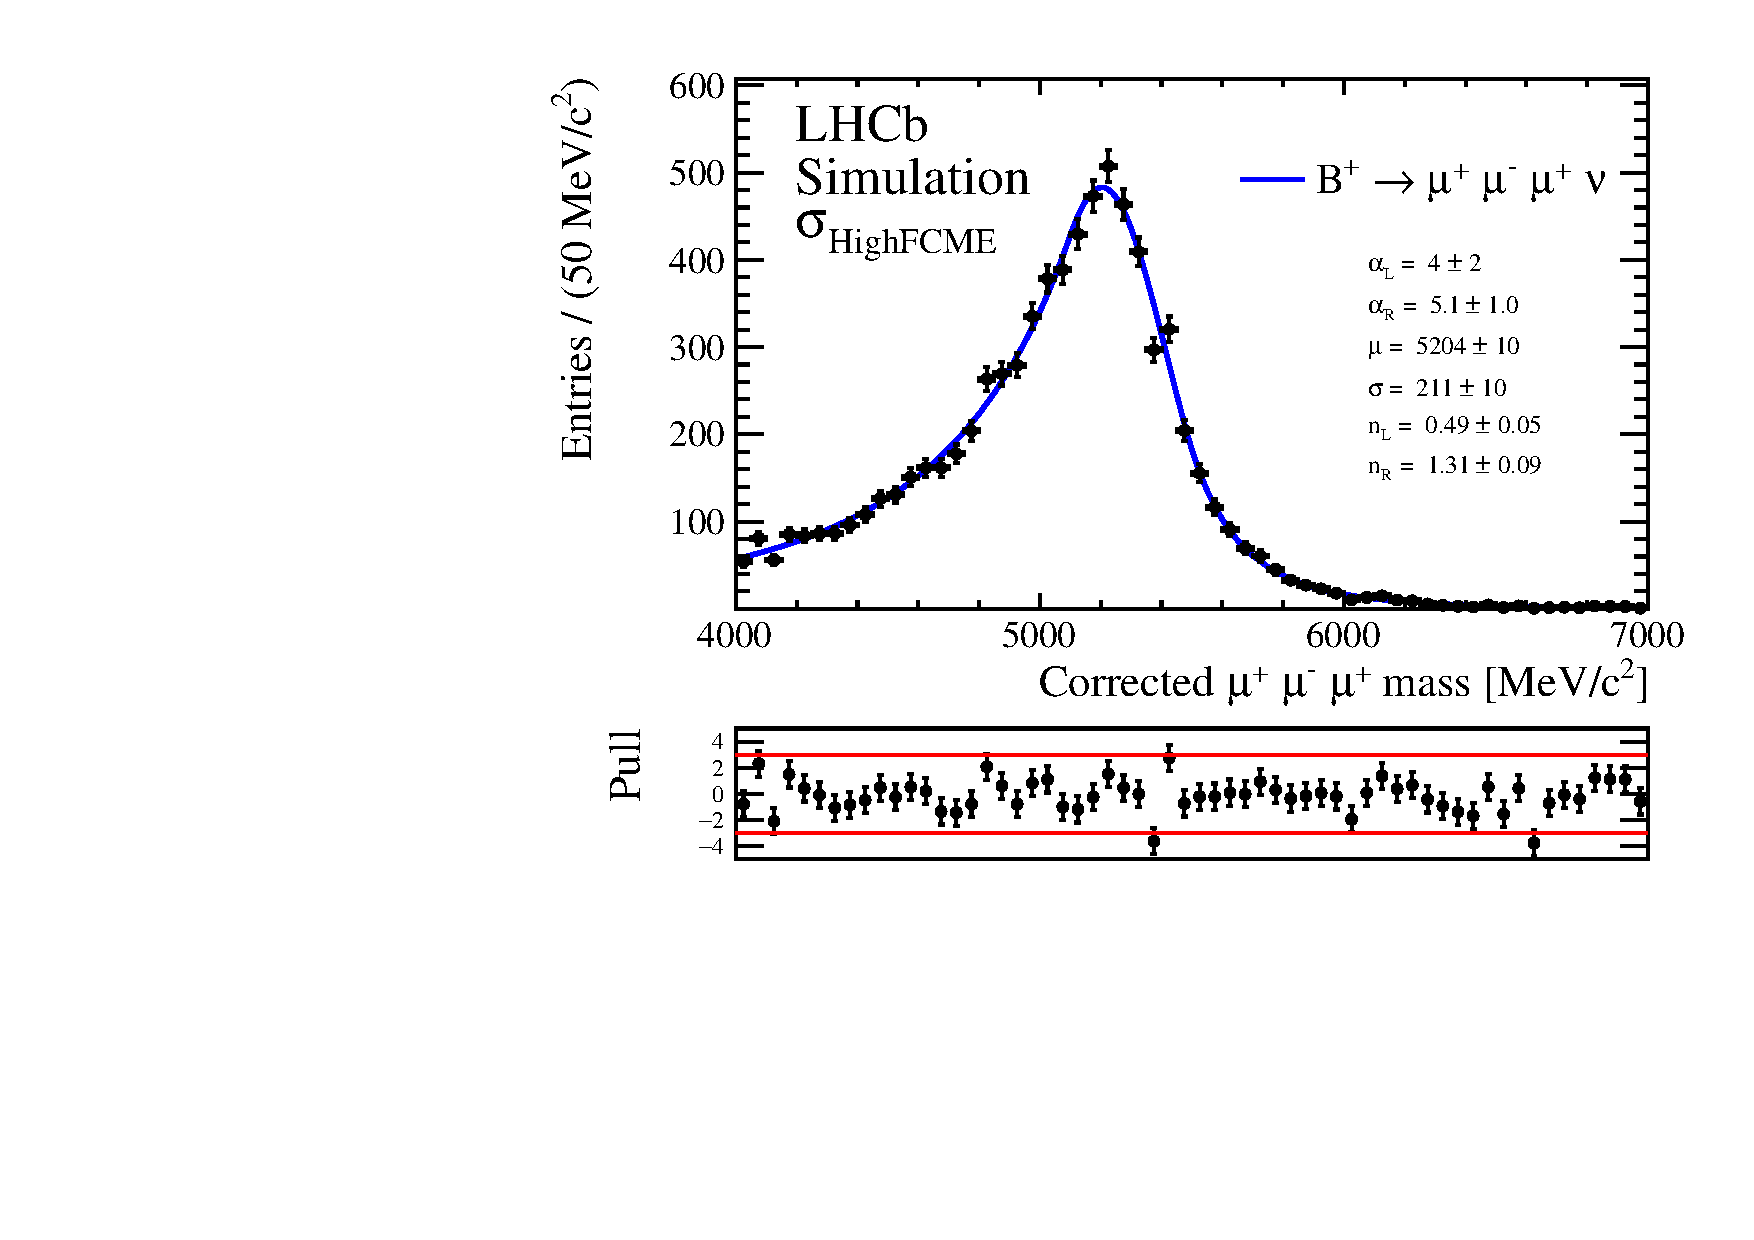
\includegraphics[width=0.5\linewidth]{./efficiency/signalfits/signalmc/sigmchighfcmeRun1nolog.pdf}\put(-30,60){(c)}%
\caption{Fit to weighted combined signal \textit{cocktail} for (a) NO FCME (b) Low FCME and (c) High FCME split.}
%\vspace*{-1.0cm}
\label{fig:MCSignalFit}
\end{figure}

\textbf{The signal yield} that is observed in the fit, $N^{sig}=N(\Bmumumu)$, is related to the branching fraction using the normalisation channel in the following way:
\begin{equation}
\begin{split}
\mathcal{B}(\Bmumumu)&=\alpha \times N(\Bmumumu)\\
&=\underbrace{\frac{\mathcal{B}(\bjpsimumuk) \times \varepsilon_{\bjpsimumuk}}{N(\bjpsimumuk) \times \varepsilon_{\Bmumumu}}}_{\text{$\alpha$}} \times N(\Bmumumu),\\
&=\underbrace{\frac{\mathcal{B}(\bjpsimumuk)}{N(\bjpsimumuk) \times  R_{\mathrm{FCME}}}}_{\text{$\alpha$}} \times N(\Bmumumu),\\
\end{split}
\label{eq:sigeq}
\end{equation}
where  $\varepsilon^{x}$ is the total selection efficiency of the channel $x$, $N_{x}$ is number of $x$ decays, $\mathcal{B}(x)$ is the branching fraction of decay $x$, $R_{\mathrm{FCME}}$ is the relevant efficiency ratio between the two decays detailed in~\autoref{EfficiencySummary} and finally $\alpha$ is the \textit{single event sensitivity}, variable which describes the sensitivity for the search. Hence, for Run \Rn{1} and Run \Rn{2} the non-simultaneous fit $N^{sig}$ is a function of six parameters $N^{sig}(R^{21}_{\mathrm{FCME}},R^{26}_{\mathrm{FCME}},N^{Run\ \Rn{1}}(\bjpsimumuk),N^{Run\ \Rn{2}}(\bjpsimumuk), \mathcal{B}(\bjpsimumuk),\mathcal{B}(\Bmumumu))$. In the simultaneous case $R^{21}_{\mathrm{FCME}}$,$R^{26}_{\mathrm{FCME}}$, $N^{Run\ \Rn{1}}(\bjpsimumuk)$ and $N^{Run\ \Rn{2}}(\bjpsimumuk) K^{+})$ is further split into $\sigma_{\mathrm{lowFCME}}$ and $\sigma_{\mathrm{highFCME}}$ bins, resulting in 10 parameters for $N^{sig}$ in the fit.



\subsubsection{Partially Reconstructed Background}
\label{finfitpr}
Partially reconstructed backgrounds are still non-negligible after the full selection chain. 
%In order to account for the contribution of the partially reconstructed backgrounds in the final signal fit, contaminating yield needs to be estimated and shape needs to be modelled. 
 The simulation sample for partially reconstructed background that originates through $D^{0}$ decays(~\autoref{partrecobak}) is used for both the yield estimate and shape modelling.

In order to get an estimate for \textbf{the yield} of these partially reconstructed decays, $N^{PR}$, \bjpsimumuk decays are again used as normalisation. Normalising to the \bjpsimumuk decay channel, the following relationship must hold: 
%This sample passed all of the selection and total selection efficiency $\varepsilon_{total}$ is listed in ~\autoref{tab:prsum}. \label{partdetailed} The Table~\ref{tab:partrecotabapp} in Appendix~\ref{partdetailed} details the efficiencies in individual steps of selection. 
%Normalising to \bjpsimumuk decay channel following relationship must hold

\begin{equation}
\begin{split}
\frac{N_{\pr}}{N_{\bjpsimumuk}}&= \frac{\mathcal{B}(\pr)}{\mathcal{B}(\bjpsimumuk)} \times \frac{\varepsilon^{\pr}}{\varepsilon^{\bjpsimumuk}} \\
&=\frac{\mathcal{B}(\pr)}{\mathcal{B}(\bjpsimumuk)} \times R_{\mathrm{FCME}},
\end{split}
\end{equation}
	where $\varepsilon^{x}$ is total selection efficiency of the channel $x$ and $R_{\mathrm{FCME}}$ is hence the efficiency ratio between the two channels, $N_{x}$ is number of $x$ decays and $\mathcal{B}(x)$ is the branching fraction of decay $x$. The quantity of interest, $N_{\pr}$, can therefore be calculated given the knowledge of all other terms. $N_{\bjpsimumuk}$ is obtained from~\autoref{tab:normchannelyields}. $\mathcal{B}(\pr)$ is obtained by multiplying $\mathcal{B}(D^{0} \rightarrow K^+ \pi^- \mu^+ \mu^{-}) = (4.17\pm0.12\pm0.40)\times 10^{-6}$\cite{Aaij:2015hva} and $\mathcal{B}(B^{+} \rightarrow D l^{+} \nu X) = (9.8 \pm 0.7)\times 10^{-2}$ \cite{Patrignani:2016xqp} yielding $\mathcal{B}(\pr) \approx (4.1\pm0.5)\times 10 ^{-7 }$. The $B^+ \rightarrow (J/\psi \rightarrow \mu^+ \mu^{-}) K^{+}$ branching fraction is obtained with the same approach: multiplying $\mathcal{B}(B^{+} \rightarrow J/\psi K^{+})$ = (1.026$\pm 0.031)\times 10^{-3}$\cite{Patrignani:2016xqp} and $\mathcal{B}(J/\psi \rightarrow \mu^{-} \mu^{+})$ = (5.961 $\pm0.0033) \times 10^{-2}$\cite{Patrignani:2016xqp} yielding 
	
\begin{equation}
\mathcal{B}(\bjpsimumuk)=(6.12\pm0.19)\times 10^{-5}.
	\label{eq:normeq}
\end{equation}


%This simulation sample all of the selection and total selection efficiency $\varepsilon_{total}$ is listed in ~\autoref{tab:prsum}. 
All the relevant total selection efficiencies are obtained from the full simulation sample and are shown in~\autoref{tab:prsum}. Due to the usage of a proxy simulation for this partially reconstructed decays (using a pion rather than a muon in one case), as discussed in~\autoref{partrecobak}, the trigger efficiency $\varepsilon_{TRG}$ cannot be obtained from simulation for partially reconstructed decays, because the \texttt{HLT2} trigger (see~\autoref{tab:triggersel}) would make positive decision only either because of finding dimuon pair or two or three-body decays, hence the trigger ratio $\frac{\varepsilon^{\pr}_{TRG}}{\varepsilon^{\bjpsimumuk}_{TRG}}$ 
is assumed to be 1, which is rather a conservative estimate (overestimate) but makes sure that other partially reconstructed backgrounds are accounted for. Another efficiency that was not accounted for because of the same reason is PID efficiency, $\varepsilon_{PID}$.
Moreover as this proxy simulation was not accessible for Run \Rn{2}, the same ratio of efficiencies as in Run \Rn{1} is used.


%$\frac{\varepsilon^{2012}_{\pr}}{\varepsilon^{2012}_{\bjpsimumuk}}=\frac{\varepsilon^{2016}_{\pr}}{\varepsilon^{2016}_{\bjpsimumuk}}$.
The summary of the expected yield is summarized in~\autoref{tab:prsum}. For the non-simultaneous final fit there are hence 5 parameters $N^{PR}(R^{21}_{\mathrm{FCME}}(\pr),N^{Run\ \Rn{1}}(\bjpsimumuk),N^{Run\ \Rn{2}}(\bjpsimumuk), \mathcal{B}(\bjpsimumuk),\mathcal{B}(\pr))$ and for the simultaneous data fit with FCME splitting 8 parameters. The total yield expected for this type of background is very low compared to the other expected backgrounds.
%Therefore to obtain number of partially reconstructed background events, $N_{\pr}$ after all selection following relationship is used: 

%\begin{equation}
%	N^{year}_{\pr}= \frac{N_{\bjpsimumuk}\times \varepsilon^{\pr}_{GEN} \times \varepsilon^{\pr}_{TOT}}{\varepsilon^{\bjpsimumuk}_{GEN}} \times \varepsilon^{\bjpsimumuk}_{TOT}
%\end{equation}



%produced in /vols/lhcb/ss4314/compare_mcpartreco_and_mcsignal/normalize_to_jpsiK/bin using the nicer figure staff

\begin{table}[ht]
\begin{center}
\begin{tabular}{ l  l  l }
\toprule
Properties & Run \Rn{1} & Run \Rn{2}  \\
\midrule
$\mathcal{B}(\pr)$ & $(4.1\pm0.5)\times 10 ^{-7 }$ &$(4.1\pm0.5)\times 10 ^{-7 }$ \\
$\mathcal{B}(\bjpsimumuk)$ &$(6.12\pm0.19)\times 10 ^{-5 }$ & $(6.12\pm0.19)\times 10 ^{-5 }$ \\
$\varepsilon^{\pr}_{total}$ &  $(1.87\pm0.04)\times 10 ^{-4 }$ & Using 2012  \\
$\varepsilon^{\bjpsimumuk}_{total}$ & $(5.80\pm0.01)\times 10 ^{-3 }$ &  Using 2012 \\
$R_{\mathrm{FCME}}^{21}(\pr)$ & $(3.22\pm0.07)\times 10 ^{-2 }$ &  Using 2012 \\
\midrule
	\multicolumn{3}{c}{{$\sigma_{\mathrm{lowFCME}}$}}  \\
$N_{\pr}$ & $19.8\pm2.6$ & $11.7\pm1.5$ \\
\midrule
	\multicolumn{3}{c}{{$\sigma_{\mathrm{highFCME}}$}}  \\
$N_{\pr}$  & $17.0\pm2.2$ & $7.9\pm1.0$ \\
\midrule
	\multicolumn{3}{c}{{$\sigma_{\mathrm{NOFCME}}$}}  \\
$N_{\pr}$ & $37.3\pm4.8$ & $20.3\pm2.6$ \\
\bottomrule
\end{tabular}
\end{center}
\caption{Summary of number of events that comes from partially reconstructed backgrounds in different bins of FCME, assuming 2012 efficiencies but extrapolating to all samples.}
\label{tab:prsum}
\end{table}

\textbf{The shape} for partially reconstructed backgrounds, $f^{PR}$, is also obtained from the simulation proxy after all the selection.
The shape is best described with the sum of two Crystal Ball functions, more in~\autoref{CB}, with free means $\mu^{1},\mu^{2}$ and widths $\sigma^{1},\sigma^{2}$ as seen in~\autoref{fig:PRFit}. Because the shape of this background suggests that the majority of the contamination is below $5000\mevcc$, it is one of the least dangerous backgrounds. In the non-simultaneous fit, $f^{PR}$ is a function of 9 parameters and for the simultaneous fit 18 parameters coming from the sum of two Crystal Ball functions. %This shape can very well describe the fit to MC with no fit range and that is why it is used here, Figure  ~\ref{fig:PartRecoFit}.


\begin{figure}[H]
\centering
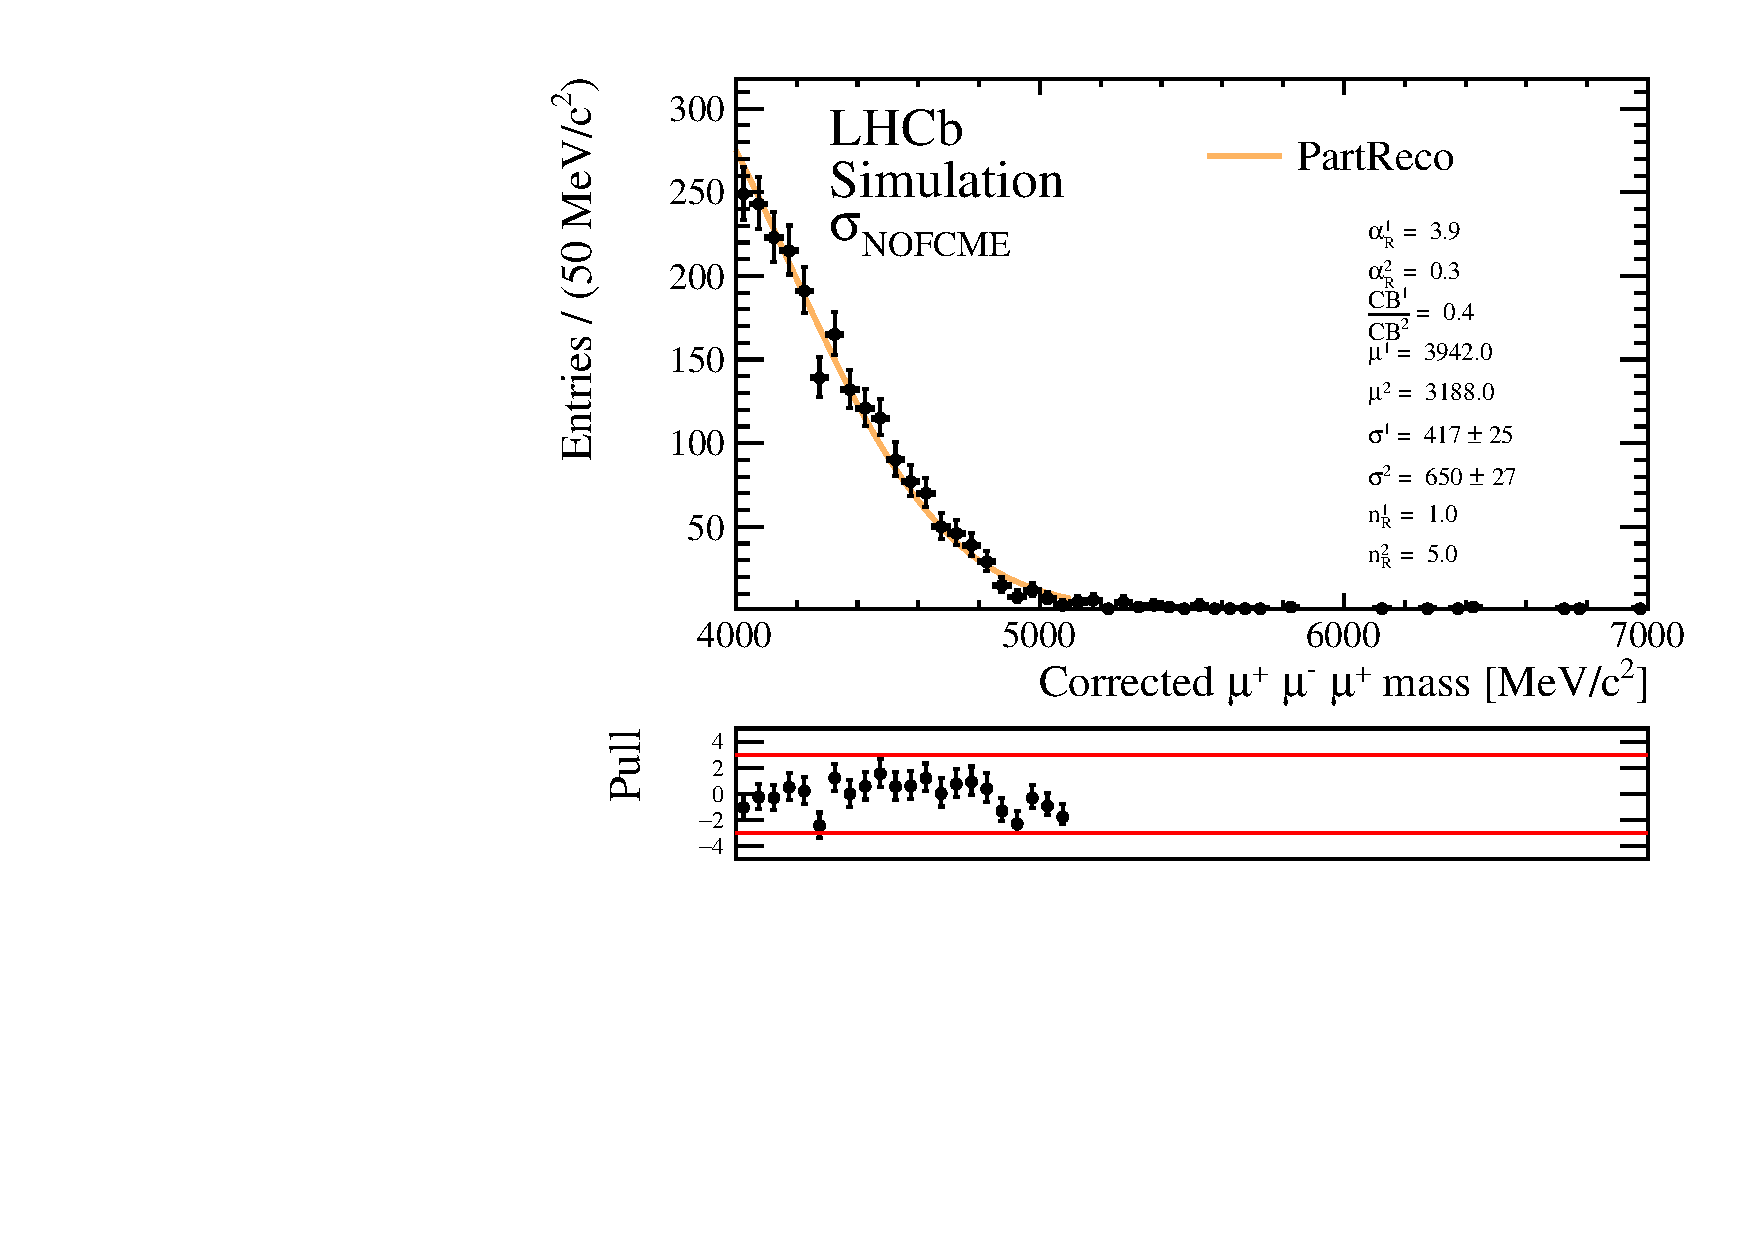
\includegraphics[width=0.5\linewidth]{./efficiency/signalfits/partrecomc/simprnofcmeRun1nolog.pdf}\put(-30,60){(a)}
\newline
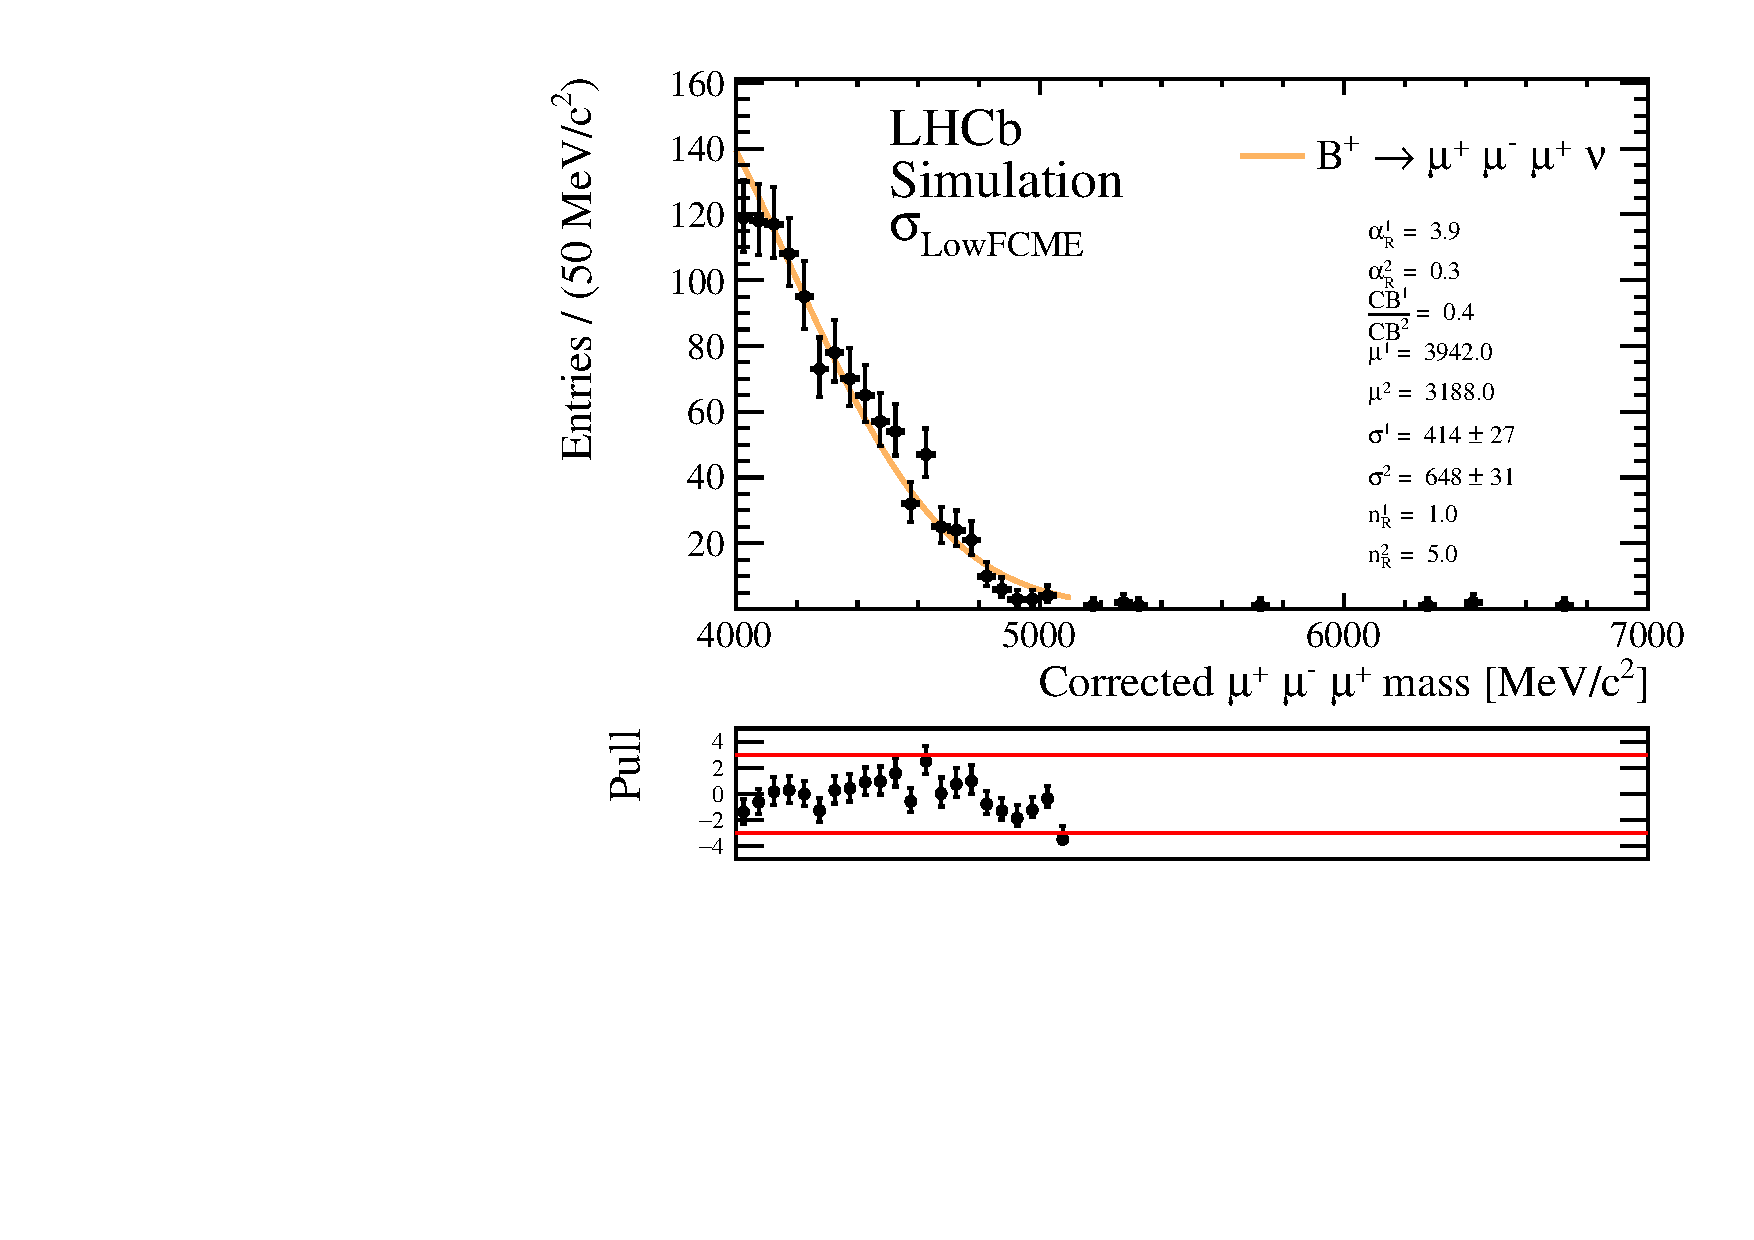
\includegraphics[width=0.5\linewidth]{./efficiency/signalfits/partrecomc/simprlowfcmeRun1nolog.pdf}\put(-30,60){(b)}%
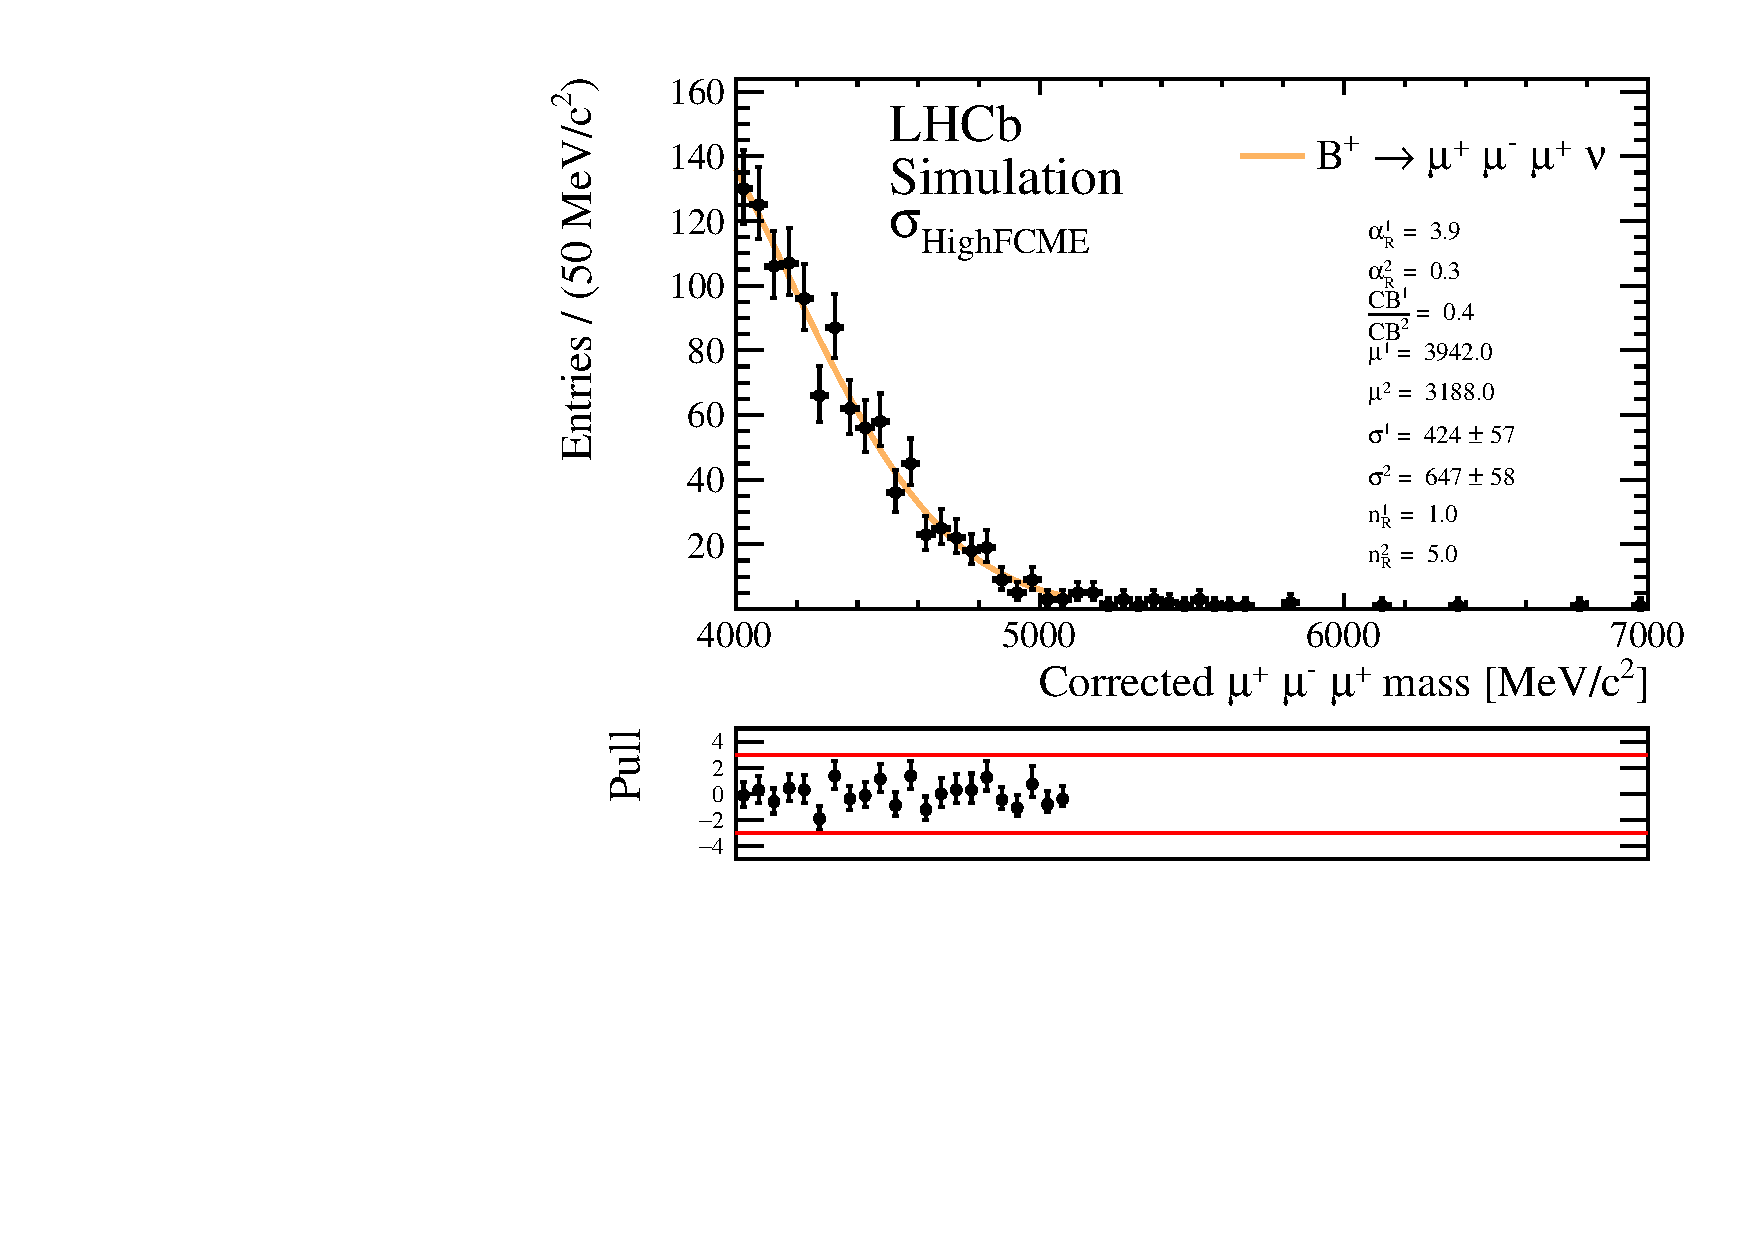
\includegraphics[width=0.5\linewidth]{./efficiency/signalfits/partrecomc/simprhighfcmeRun1nolog.pdf}\put(-30,60){(c)}%
\caption{Fit to weighted combined partially reconstructed background simulation proxy for (a) NO FCME (b) Low FCME and (c) High FCME split.}
%\vspace*{-1.0cm}
\label{fig:PRFit}
\end{figure}

\subsubsection{MisID background}
\label{misidfitstrat}
The level and the shape of misID background is determined by fitting the misID data samples obtained using the method described in~\autoref{misidprocedure}. A binned $\chi^{2}$ fit is used to extract the shape and yields parameters. The reason for usage of the binned $\chi^{2}$ fit is that the misID samples are low-statistics weighted samples and the shape and yield needs to be propagated to the final data fit while preserving the fit parameter correlations. Since there is a prescale factor of 1\% at stripping level, to obtain the correct yield, the final number needs to be multiplied by 100 to counteract the prescale.

The misID weights obtained from kinematically binned \bjpsikst samples (see ~\autoref{extraction}) have uncertainties associated with them as shown in Figures~\ref{fig:JpsiKnew},~\ref{fig:JpsiKaonnew},~\ref{fig:JpsiPionnew2016},~\ref{fig:JpsiKaonnew2016}. These uncertainties are accounted for in the fit by Gaussian variation of the weights within the uncertainty in a given kinematic bin of $p,\eta$ for each particle species and then folded in to the misID calculation. In this case 100 variations were used. Each variation results in a different template for the misID shape. This misID template is then subsequently binned in 15 bins of corrected mass. From each corrected mass bin, mean $\mu_{var}$ and error $\sigma_{var}$ from gaussianly distributed number of misID events is obtained. 

The total uncertainty due to the weight, $\sigma_{tot}$, for a given bin of corrected mass is calculated using $\sqrt{\sigma_{var}^2 +\sqrt{\sum{w^{2}_{i}}}^{2}}$, where $\sigma_{par}=\sqrt{\sum{w^{2}_{i}}}$ is the associated error per bin and $\sigma_{var}$ is the standard deviation obtained from variation of misID weights. Finally, The binned $\chi^{2}$ fit is made to the misID samples with the total uncertainty. \textbf{The number of misID events}, $N^{MisID}$, for different species-regions after all selections are seen in~\autoref{tab:misidtabcummu}. Hence for the non-simultaneous fit this just add 1 parameter and for the simultaneous fit there will be two parameters describing the total yield of misID.

Also it can be seen in~\autoref{tab:misidtabcummu}, crossfeedweight is only considered for kaon-like and pion-like \textit{SS misID} samples. This arises as a consequence of two characteristics of the misID crossfeedweight procedure. First the convergence criteria makes unbalanced samples (one sample very high in misID events and other sample very small in number of misID events) hard to satisfy (case for most of \textit{OS misID} samples). Secondly, proton-like region samples are very sparse and hence it is not necessary to account for crossfeed. %, see Figure ~\ref{fig:ProtonPIDHeatMap}.

The binned $\chi^{2}$ fits using a Crystal Ball function to different bins of FCME is performed as seen in~\autoref{fig:MisidFinalFit}. This means that \textbf{the shape} of this background, $f^{MisID}$, is a function of 4 parameters in the non-simultaneous case and a function of 8 parameters in the simultaneous case. Both full weight error $\sigma_{tot}$ and partial weight error $\sigma_{par}$ are plotted. The difference between the two, is the error due to uncertainty on the weight $\sigma_{var}$.  Results of the fits are propagated into the signal data fits preserving correlations between parameters, which are hence a set if multidimensional gaussian constraints in the signal data fits. This means that all uncertainties due to misID will be directly accounted for in the signal data fits.


\begin{table}[H]
%\small
\begin{center}
\begin{tabular}{ l  l  l  l  l  }
\toprule
Sample & Region & PID & weight & misID count  \\
% &  &  &  & misID count \\
\midrule
Run \Rn{1} \textit{SS misID} & Kaon-region & Run \Rn{1} PID & crossfeedweight & 198 \\
Run \Rn{1} \textit{SS misID} & Pion-region  &  & crossfeedweight & 103 \\
Run \Rn{1} \textit{SS misID} & Proton-region &  & no-crossfeedweight & 6 \\
Run \Rn{1} \textit{OS misID} & Kaon-region &  & no-crossfeedweight & 3 \\
Run \Rn{1} \textit{OS misID} & Pion-region &  & no-crossfeedweight & 42 \\
Run \Rn{1} \textit{OS misID} & Proton-region &  & no-crossfeedweight & 1 \\
Run \Rn{2} \textit{SS misID} & Kaon-region & Run \Rn{2} PID  & crossfeedweight & 136 \\
Run \Rn{2} \textit{SS misID} & Pion-region &  & crossfeedweight & 76 \\
Run \Rn{2} \textit{SS misID} & Proton-region &  & no-crossfeedweight & 0 \\
Run \Rn{2} \textit{OS misID} & Kaon-region &  & no-crossfeedweight & 8 \\
Run \Rn{2} \textit{OS misID} & Pion-region &  & no-crossfeedweight & 45 \\
Run \Rn{2} \textit{OS misID} & Proton-region &  & no-crossfeedweight & 1 \\\hline
	Sum & & & & 619\\
\bottomrule
\end{tabular}
\end{center}
	\caption{The final misID template is constructed by summing the contribution from Run \Rn{1} and \Rn{2} kaon, pion and proton-like regions for both \textit{SS} and \textit{OS misID} contributions. }%The last column adds cumulatively the contributions with respect to the previous row. }
\label{tab:misidtabcummu}
\end{table}

\begin{figure}[H]
\centering
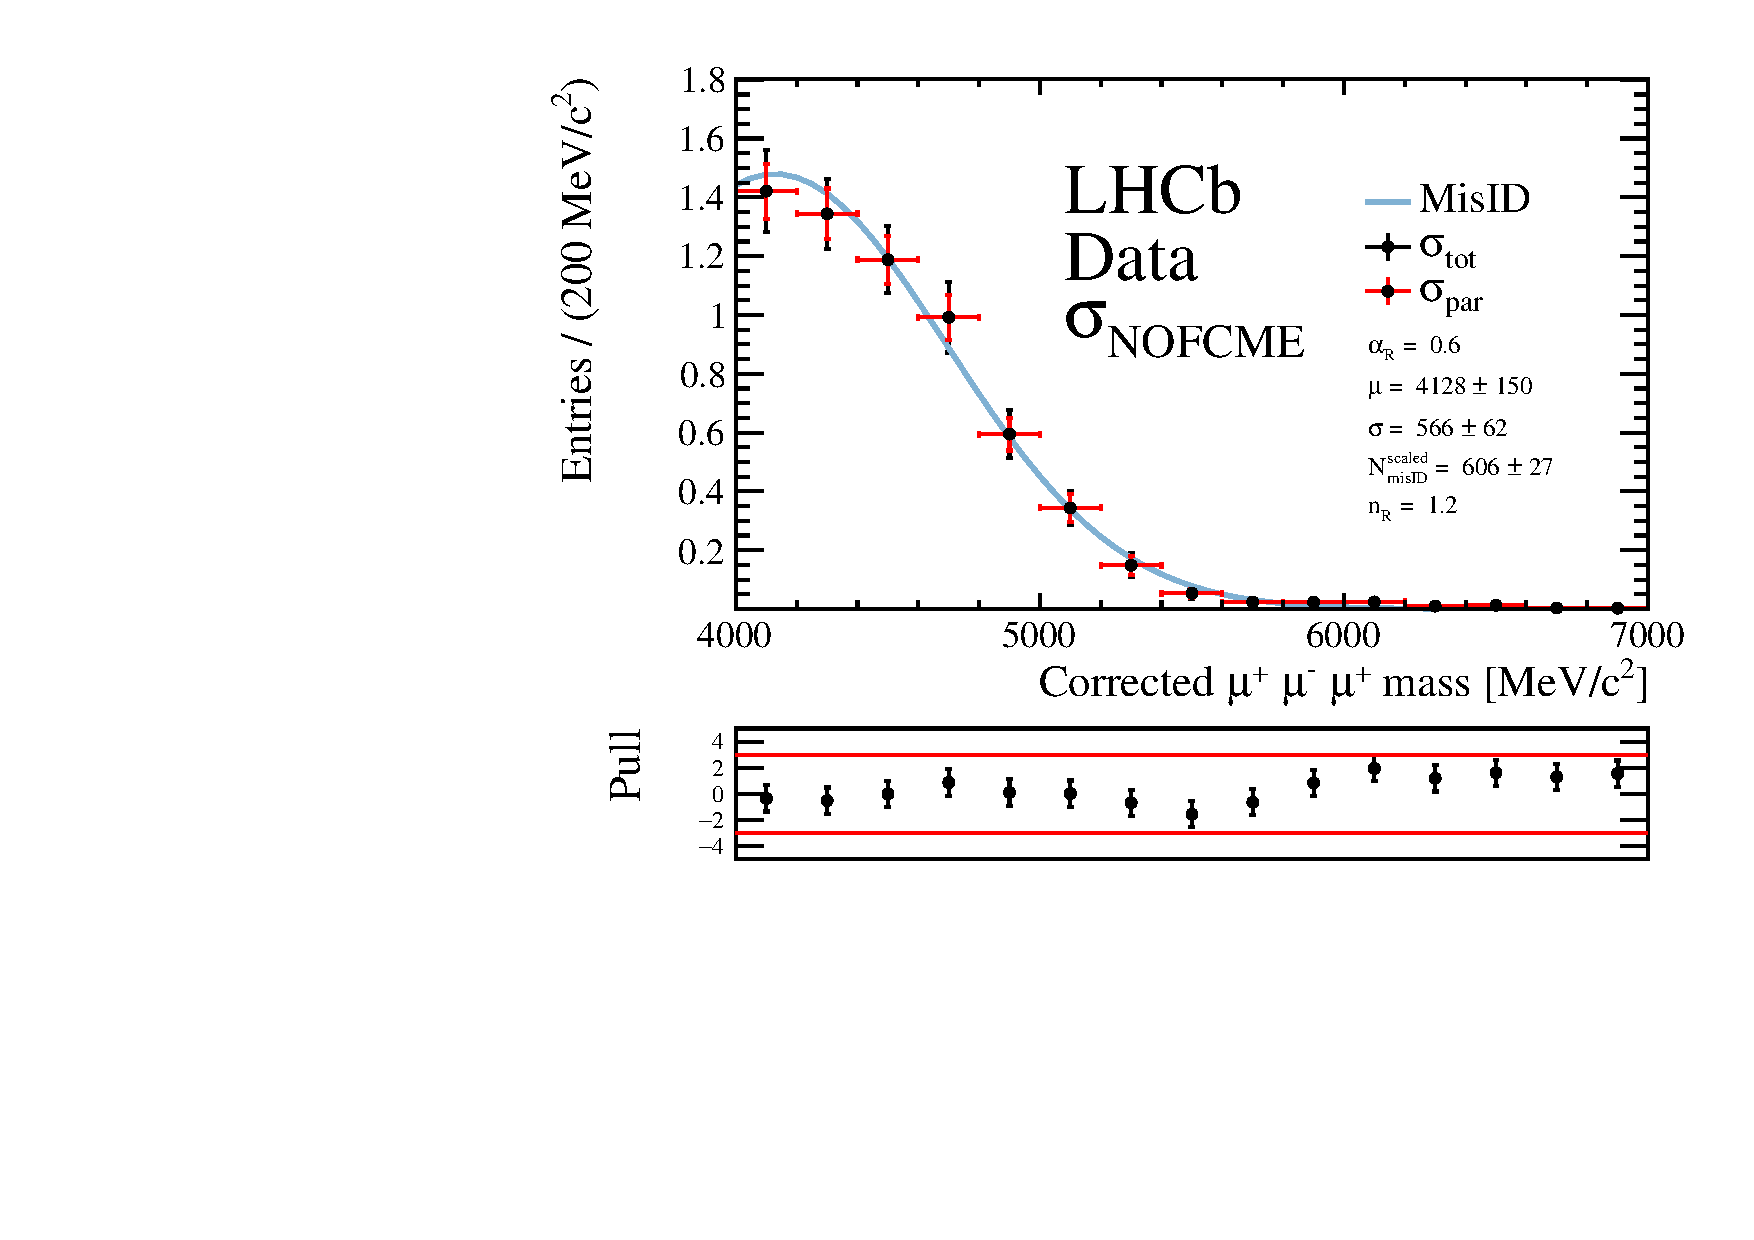
\includegraphics[width=0.5\linewidth]{./efficiency/signalfits/misiddata/misiddatanofcmeRun1nolog.pdf}\put(-30,60){(a)}
\newline
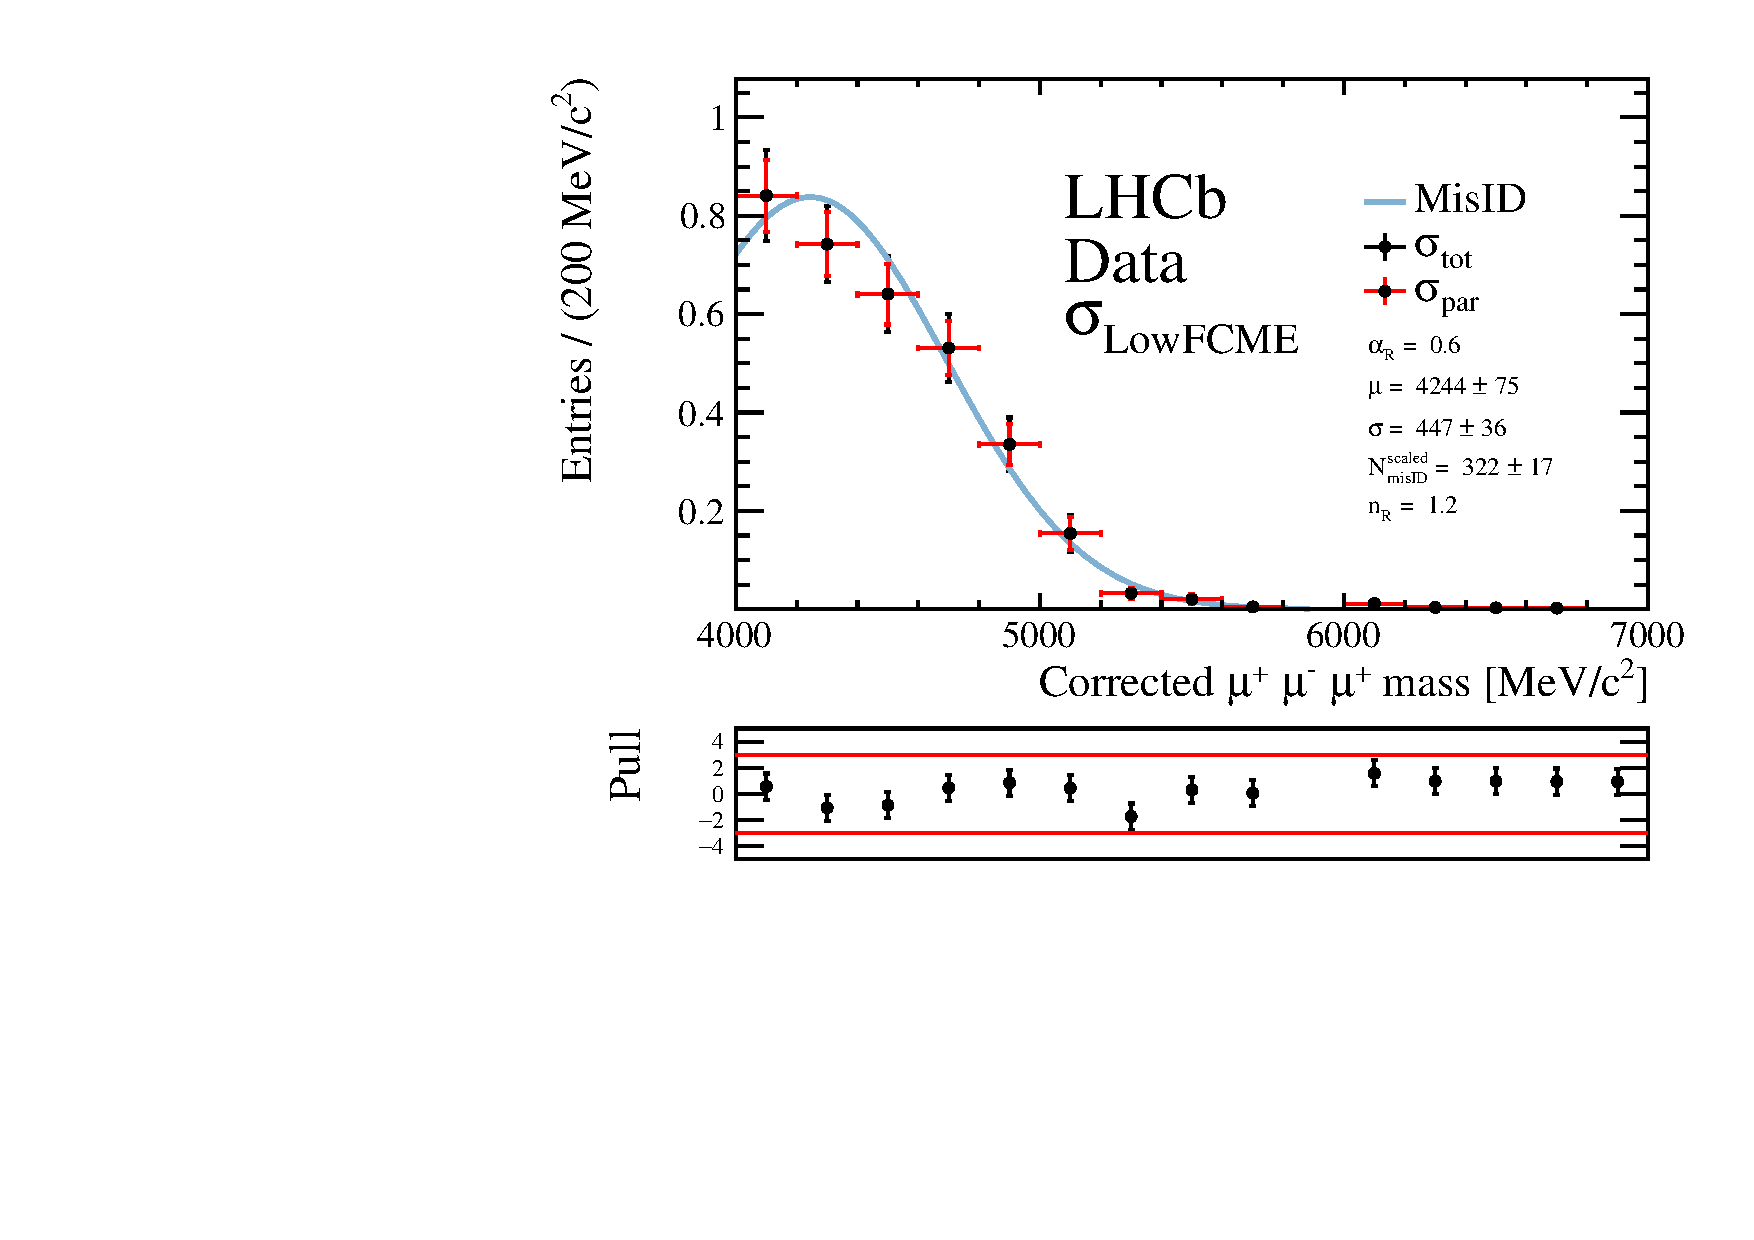
\includegraphics[width=0.5\linewidth]{./efficiency/signalfits/misiddata/misiddatalowfcmeRun1nolog.pdf}\put(-30,60){(b)}%
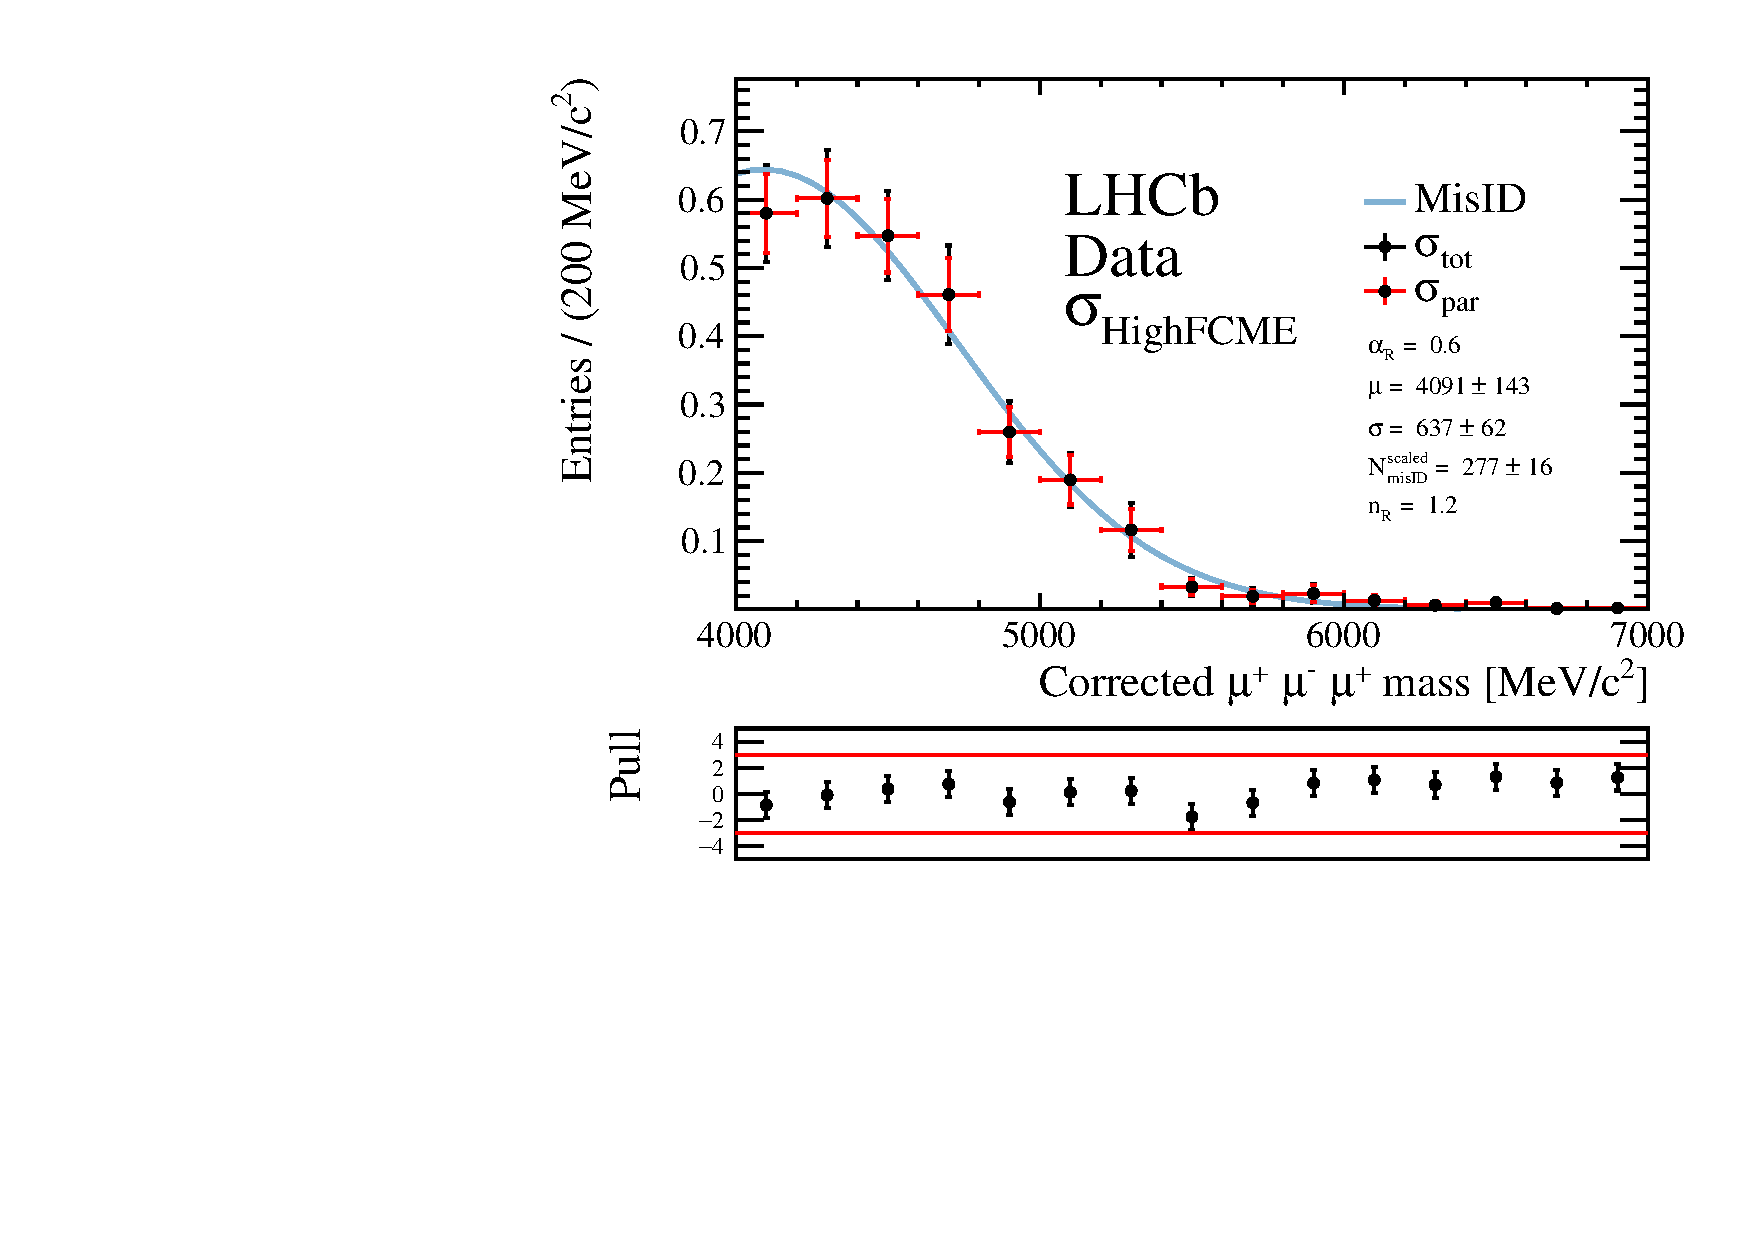
\includegraphics[width=0.5\linewidth]{./efficiency/signalfits/misiddata/misiddatahighfcmeRun1nolog.pdf}\put(-30,60){(c)}%
	\caption{Binned $\chi^{2}$ fit to the misID templates with no FCME split (b) Low FCME (c) High FCME. In high FCME bin, the distribution of misID is pollutes signal window more than in the low FCME bin. Both full weight error $\sigma_{tot}$ and partial weight error $\sigma_{par}$ can be seen.}
%\vspace*{-1.0cm}
\label{fig:MisidFinalFit}
\end{figure}

\subsubsection{Combinatorial Background}
The signal data fit so far includes components for signal component, partially reconstructed background component, and misID background component. The only component left to estimate is the combinatorial background. To model the combinatorial component, the exponential function is left floating and fit to data, which was motivated in~\autoref{combiback}. Hence \textbf{the shape}, $f^{Combi}$, has one(two) parameter(s) for the non-simultaneous(simultaneous) fit, which is the exponential constant. And \textbf{the yield}, $N^{Combi}$, is also parametrised just with one (two) parameter(s) for non-simultaneous (simultaneous) fit.

%\subsection{Signal Data Fit}
%\label{fitsens}
%
%There are two types of fits that are performed to signal data. Firstly, \textbf{blinded signal data fit} is performed in order to evaluate the expected sensitivity and is only fitted to blinded signal data. Secondly \textbf{full signal data fit} is performed to perform the measurement for setting the limit on the $\mathcal{B}(\Bmumumu)$.
%
%
%\subsection{Signal Channel Fit}
%\label{Fit}
%A simultaneous unbinned maximum likelihood fit to the $\mu^{+} \mu^{-} \mu^{+}$ corrected mass spectrum to combined Run \Rn{1} and \Rn{2} dataset after the full selection in two bins of fractional corrected mass error is performed. As the corrected mass error have a dependence on resolution as mentioned in~\autoref{split}, this split will increase sensitivity. Shapes and yields used for different components of the signal corrected mass fits will be described in this sections. As it will be shown, the components are constrained using either by using data driven methods or simulated samples. As non-simultaneous fit is used as a cross-check its parametrisation is described as well.
%
%Throughout the analysis there was a \textbf{blinding procedure} in place where the signal region $4500\mevcc <M_{\mathrm{B_{corr}}}<5500\mevcc$ was blinded. Hence in the blinded data fits this region is omitted. In this blinded unbinned likelihood fit to the data, the shapes and yields are extrapolated to the blinded region in order to asses sensitivity, summarized in ~\autoref{fitsens}\mybox{\color{red} sensitivity}. Upon unblinding unbinned likelihood fit to full data is perfomed with signal yield floating and mean $\mu_{sig}$ and width $\sigma_{sig}$ constrained from simulation.
%
%\subsubsection{Signal}
%The full fit to Run \Rn{1} and Run \Rn{2} data requires the signal shape knowledge for combined dataset. This is obtained fromRun \Rn{1} and Run \Rn{2} signal simulation \textit{cocktail}. The cocktail is created after full selection by assigning event-by-event weights, \textit{$w^{i}$}, which capture the differences between Run \Rn{1} and Run \Rn{2} simulation, that ware not considered by full selection.
%
%Firstly, weights that reflect the expected difference due to increased luminosity are computed. To obtain these signal weights, following conditions must be satisfied
%
%%Signal shape for Run \Rn{1} and Run \Rn{2} is described by probability density function (P.D.F) in corrected mass taken from $B^{+} \rightarrow \mu^{+} \mu^{-} \mu^{+} \nu_\mu$ 2012 MC and 2016 MC cocktail. After all respective
%%selection, this cocktail is created by assigning event-by-event weights. Signal event-by-event weights, \textit{$w^{i}$}, to create cocktail come from differences between 2012 MC and 2016 MC. To obtain signal weights, following conditions must be satisfied,
%\begin{equation}
%n^{2012}=\mathcal{L}^{2012} \times \sigma^{2012}_{pp \rightarrow b \overline{b}},
%\end{equation}
%
%\begin{equation}
%n^{2016}=\mathcal{L}^{2016} \times \sigma^{2016}_{pp \rightarrow b \overline{b}},
%\end{equation}
%
%\begin{equation}
%w^{2012} \times N^{2012} + w^{2016} \times N^{2016} = N^{2012} + N^{2016},
%\end{equation}
%
%\begin{equation}
%\frac{w^{2012} \times N^{2012}}{w^{2016} \times N^{2016}} = \frac{n^{2012}}{n^{2016}}.
%\end{equation}
%
%These constraints yield following value for event-by-event (or rather yearly) weights
%
%
%\begin{equation}
%w^{2012}= \frac{N^{2012}+N^{2016}}{N^{2012}\times(1.0+\frac{n^{2016}}{n^{2012}})}=0.931
%\end{equation}
%
%
%\begin{equation}
%w^{2016}= \frac{N^{2016}+N^{2012}}{N^{2016}\times(1.0+ \frac{n^{2012}}{n^{2016}})}=1.073,
%\end{equation}
%
%
%
%where $N^{2012},N^{2016}$ number of events at \textit{generator level}, $\mathcal{L}^{2012},\mathcal{L}^{2016}$ are integrated luminosities, and $\sigma^{2012}_{pp \rightarrow b \overline{b}}, \sigma^{2016}_{pp \rightarrow b \overline{b}}$ are cross-sections in a given year. $N^{2012},N^{2016}$ number of events at \textit{generator level} is obtained by dividing number of reconstructed events $N_{REC}$ by the reconstruction efficiency $\varepsilon_{REC}$ (see~\autoref{tab:effsumarry}). Values for these variables are summarized in ~\autoref{tab:MCweightNOFCME}.
%
%
%\begin{table}[h]
%\centering
%\begin{tabular}{ l  c  c }
%\toprule
%Summary & 2012 Simulation & 2016 Simulation \\
%\midrule
%%$\epsilon_{PID}$ & taken from PID & taken from PID  \\
%%$\epsilon_{GEN}$  & 0.18643$\pm$0.00029 & 0.1977$\pm$0.0004 \\
%
%
%$N_{REC}$  & 1114130 & 1107715 \\
%$\mathcal{L}$ & 2968 $\rm{pb^{-1}}$ & 1612 $\rm{pb^{-1}}$ \\
%$\sigma_{pp \rightarrow b \overline{b}}$ & 1 & 2  \\
%\bottomrule
%\end{tabular}
%	\caption{Signal simulation weights used to create cocktail of mixed Run \Rn{1} (2012) and Run \Rn{2} (2016) cocktail. The cross-sections listed here are not absolute numbers, but rather relative as only its ratio matters.}
%\label{tab:MCweightNOFCME}
%\end{table}
%
%Secondly, event-by-event weight which differs between Run \Rn{1} and \Rn{2} that need to be accounted is PID efficiency $\varepsilon_{PID}$ (see~\autoref{tab:effsumarry}), which depends on the kinematics of the final state particles. It is denoted as $w^{i\varepsilon\{2012,2016\}}_{\varepsilon^{i}_{PID}}$. 
%
%The final weight of an event depending on Run \Rn{1} and Run \Rn{2} is calculated 
%
%\begin{equation}
%	w^{i\varepsilon\{2012,2016\}}_{total}=  w^{i\varepsilon\{2012,2016\}} \times w^{i\varepsilon\{2012,2016\}}_{\varepsilon^{i}_{PID}}.
%\end{equation}
%
%After obtaining combined Run \Rn{1} and \Rn{2} signal \textit{cocktail}, fit to this weighted simulation is done with \textbf{the shape} in the corrected mass modelled by double-sided Crystal Ball function~\autoref{IP}. Fit and its parameters can be seen in~\autoref{fig:MCSignalFit}. The function describing this shape is denoted as $f^{sig}$ and hence is a function 6 parameters for non-simultaneous fit and 12 parameters for simultaneous fit.
%
%\begin{figure}[H]
%\centering
%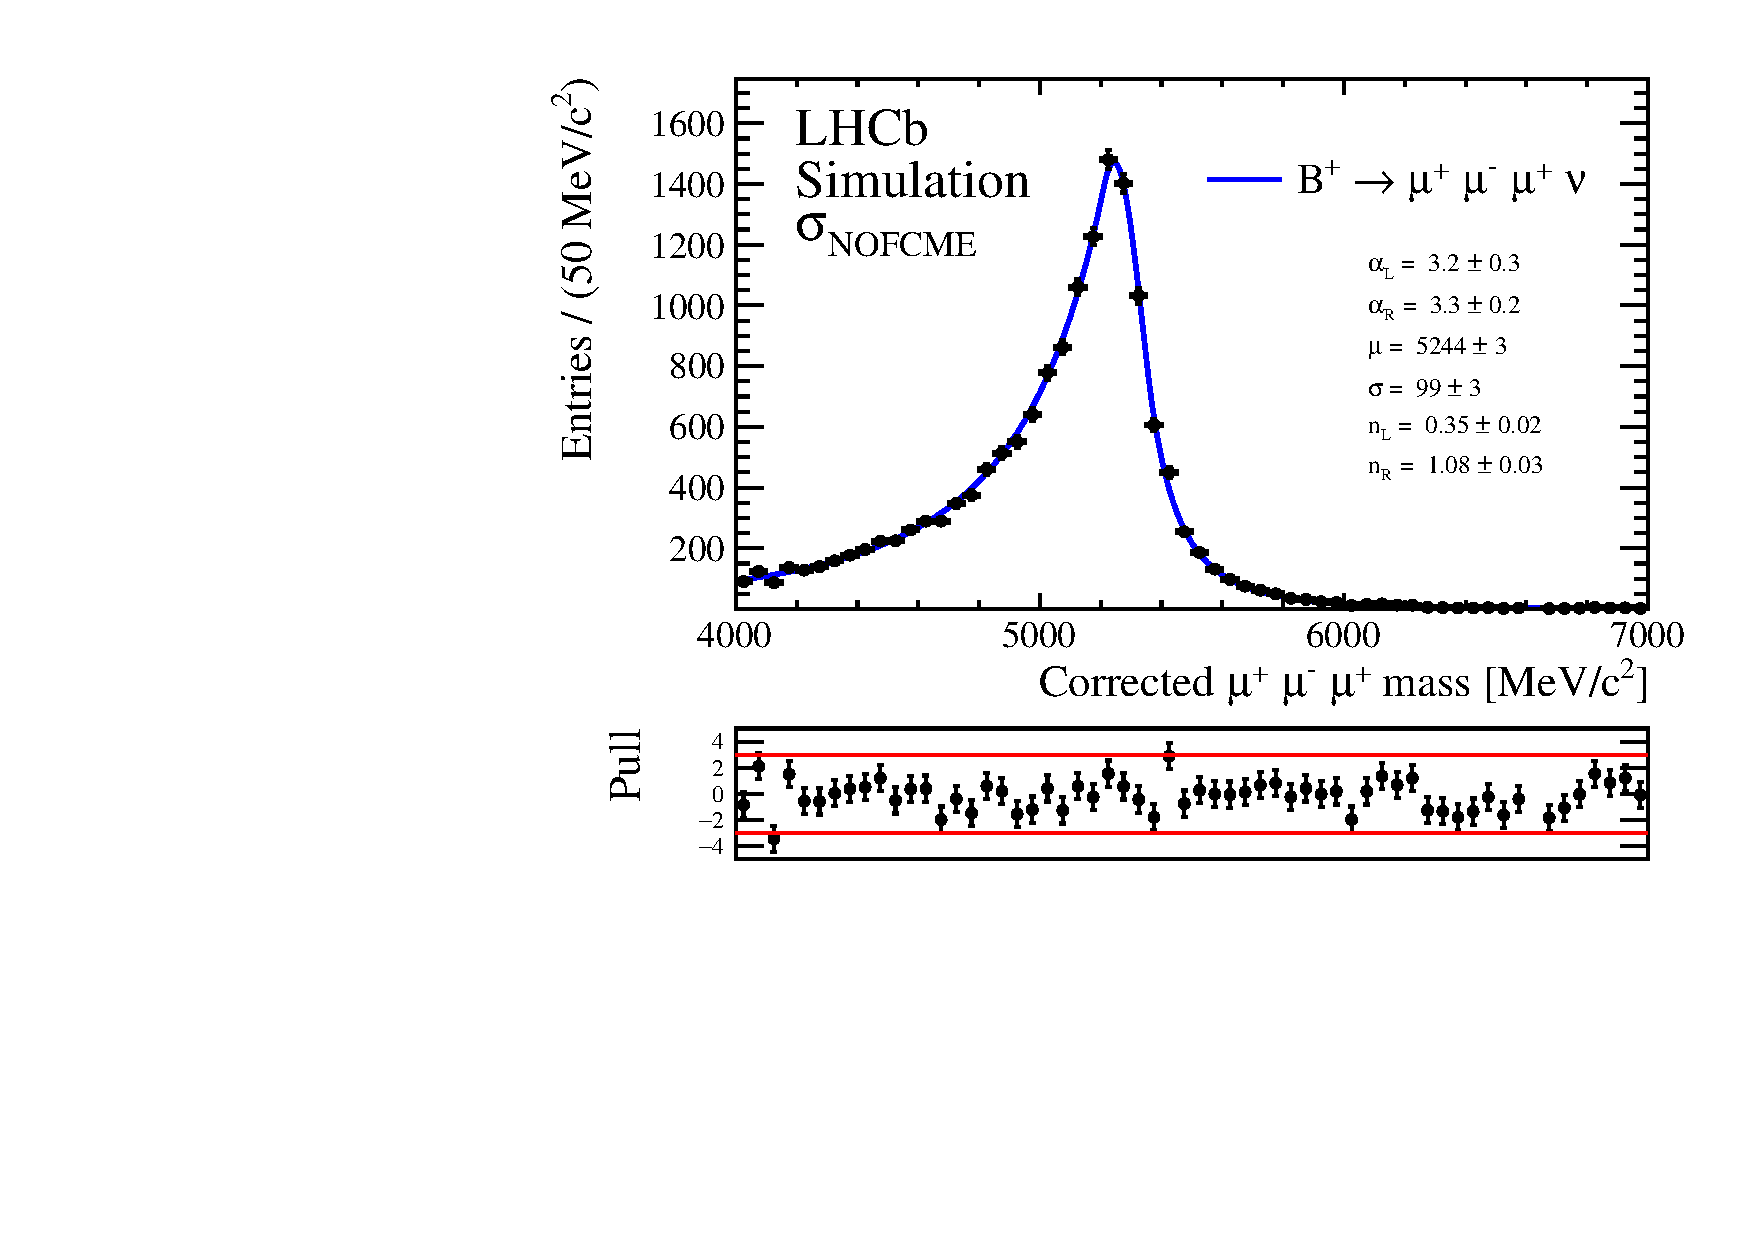
\includegraphics[width=0.5\linewidth]{./efficiency/signalfits/signalmc/sigmcnofcmeRun1nolog.pdf}\put(-30,60){(a)}
%\newline
%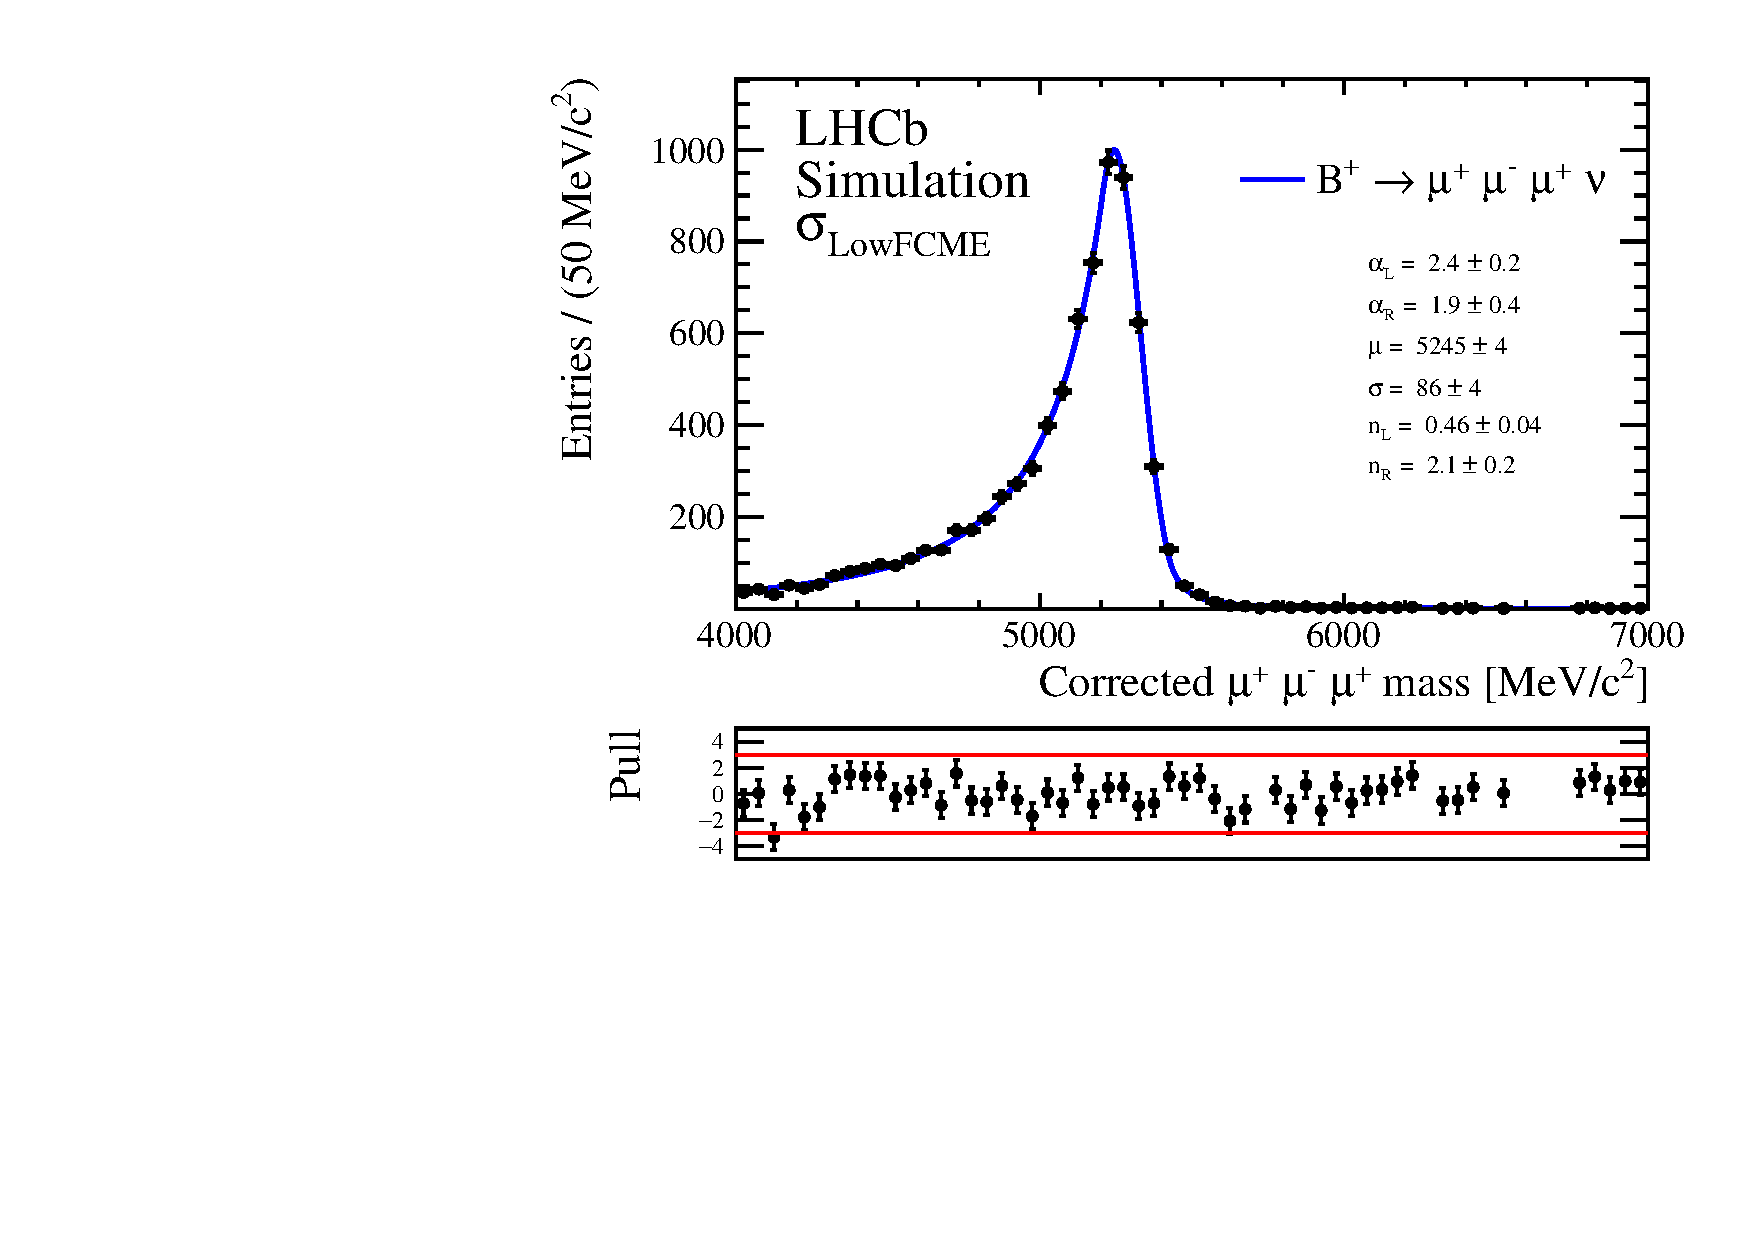
\includegraphics[width=0.5\linewidth]{./efficiency/signalfits/signalmc/sigmclowfcmeRun1nolog.pdf}\put(-30,60){(b)}%
%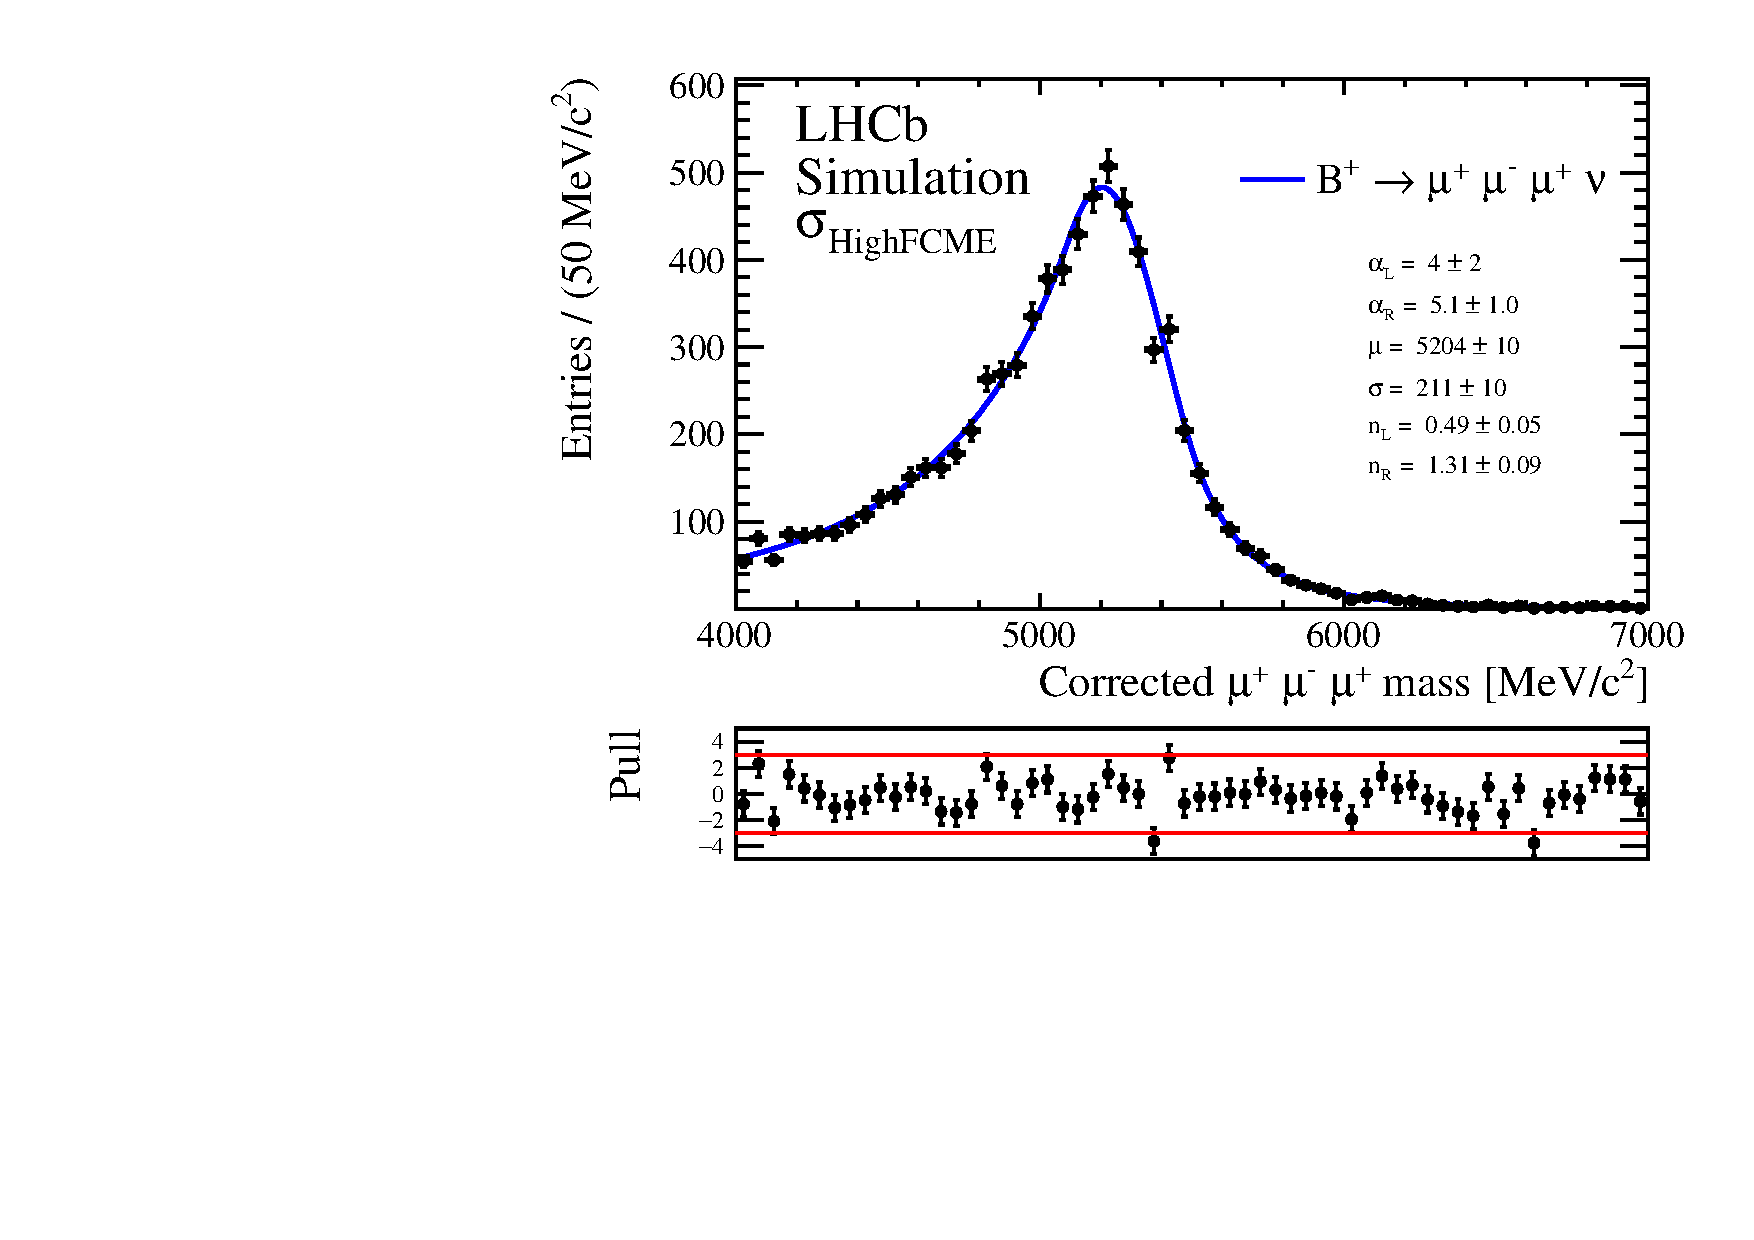
\includegraphics[width=0.5\linewidth]{./efficiency/signalfits/signalmc/sigmchighfcmeRun1nolog.pdf}\put(-30,60){(c)}%
%\caption{Fit to weighted combined signal \textit{cocktail} for (a) NO FCME (b) Low FCME and (c) High FCME split.}
%%\vspace*{-1.0cm}
%\label{fig:MCSignalFit}
%\end{figure}
%
%\textbf{The signal yield} that is observed in the fit, $N^{sig}=N(\Bmumumu)$, is related to the branching fraction using normalisation channel in a following way:
%\begin{equation}
%{\mathcal{B}(\Bmumumu)}=\alpha \times N(\Bmumumu)
%\end{equation}
%\begin{equation}
%	=\underbrace{\frac{\mathcal{B}(\bjpsimumuk) \times \varepsilon_{\bjpsimumuk}}{N(\bjpsimumuk) \times \varepsilon_{\Bmumumu}}}_{\text{$\alpha$}} \times N(\Bmumumu),
%\end{equation}
%\begin{equation}
%	=\underbrace{\frac{\mathcal{B}(\bjpsimumuk)}{N(\bjpsimumuk) \times  R_{\mathrm{FCME}}}}_{\text{$\alpha$}} \times N(\Bmumumu),
%\end{equation}
%where  $\varepsilon^{x}$ is total selection efficiency of $x$ channel, $N_{x}$ is number of $x$ decays, $\mathcal{B}(x)$ is the branching fraction of decay $x$, $R_{\mathrm{FCME}}$ is the relevant efficiency ratio between two decays detailed in~\autoref{EfficiencySummary} and finally $\alpha$ is the \textit{single event sensitivity}, variable which desribes the sensitivity for the search. Hence for Run \Rn{1} and Run \Rn{2} altogether for non-simultaneous fit $N^{sig}$ is a function of six parameters $N^{sig}(R^{21}_{\mathrm{FCME}},R^{26}_{\mathrm{FCME}},N^{Run\ \Rn{1}}(\bjpsimumuk),N^{Run\ \Rn{2}}(\bjpsimumuk), \mathcal{B}(\bjpsimumuk),\mathcal{B}(\Bmumumu))$. In  simultaneous case $R^{21}_{\mathrm{FCME}}$,$R^{26}_{\mathrm{FCME}}$, $N^{Run\ \Rn{1}}(\bjpsimumuk)$ and $N^{Run\ \Rn{2}}(\bjpsimumuk) K^{+})$ is further split into $\sigma_{lowFCME}$ and $\sigma_{highFCME}$ bins, resulting in 10 parameters for $N^{sig}$ in the fit.
%
%
%
%\subsubsection{Partially Reconstructed Background}
%\label{finfitpr}
%Partially reconstructed backgrounds are still non-negligible after full selection chain. In order to account for the contribution of the partially reconstructed backgrounds in the final signal fit, contaminating yield needs to be estimated and shape needs to be modelled. Simulation sample for partially reconstructed background that originates through $D^{0}$ was described in~\autoref{partrecobak} is used for both the yield estimate and shape modelling.
%
%In order to get estimate for \textbf{the yield} of these partially reconstructed decays, $N^{PR}$, \bjpsimumuk decays are again used as normalisation. Normalising to \bjpsimumuk decay channel following relationship must hold 
%%This sample passed all of the selection and total selection efficiency $\varepsilon_{total}$ is listed in ~\autoref{tab:prsum}. \label{partdetailed} The Table~\ref{tab:partrecotabapp} in Appendix~\ref{partdetailed} details the efficiencies in individual steps of selection. 
%%Normalising to \bjpsimumuk decay channel following relationship must hold
%
%\begin{equation}
%\begin{split}
%\frac{N_{\pr}}{N_{\bjpsimumuk}}&= \frac{\mathcal{B}(\pr)}{\mathcal{B}(\bjpsimumuk)} \times \frac{\varepsilon^{\pr}}{\varepsilon^{\bjpsimumuk}} \\
%&=\frac{\mathcal{B}(\pr)}{\mathcal{B}(\bjpsimumuk)} \times R_{\mathrm{FCME}},
%\end{split}
%\end{equation}
%	where $\varepsilon^{x}$ is total selection efficiency of $x$ channel and $R_{\mathrm{FCME}}$ is hence the efficiency ratio between the two channels, $N_{x}$ is number of $x$ decays, $\mathcal{B}(x)$ is the branching fraction of decay $x$. The quantity of interest, $N_{\pr}$, can be therefore calculated given the knowledge of all other terms. $N_{\bjpsimumuk}$ is was obtained from~\autoref{tab:normchannelyields}. $\mathcal{B}(\pr)$ is obtained by amalgamating $\mathcal{B}(D^{0} \rightarrow K^+ \pi^- \mu^+ \mu^{-}) = (4.17\pm0.12\pm0.40)\times 10^{-6}$\cite{Aaij:2015hva} and $\mathcal{B}(B^{+} \rightarrow D l^{+} \nu X) = (9.8 \pm 0.7)\times 10^{-2}$ \cite{Patrignani:2016xqp} yielding $\mathcal{B}(\pr) \approx (4.10\pm0.50)\times 10 ^{-7 }$. $B^+ \rightarrow (J/\psi \rightarrow \mu^+ \mu^{-}) K^{+}$ branching fraction is obtained with the same approach: multiplying $\mathcal{B}(B^{+} \rightarrow J/\psi K^{+})$ = (1.026$\pm 0.031)\times 10^{-3}$\cite{Patrignani:2016xqp} and $\mathcal{B}(J/\psi \rightarrow \mu^{-} \mu^{+})$ = (5.961 $\pm0.0033) \times 10^{-2}$\cite{Patrignani:2016xqp} yielding $\mathcal{B}(\bjpsimumuk)=(6.12\pm0.19)\times 10^{-5}$.
%
%
%
%%This simulation sample all of the selection and total selection efficiency $\varepsilon_{total}$ is listed in ~\autoref{tab:prsum}. 
%All the relevant total selection efficiencies are obtained from the full simulation sample and are shown in~\autoref{tab:prsum}. Due to the usage of a proxy simulation for this partially reconstructed decays (using a pion rather than a muon in one case), as discussed in~\autoref{partrecobak}, trigger efficiency $\varepsilon_{TRG}$ cannot be obtained from simulation for partially reconstructed decays, because the \texttt{HLT2} trigger (see~\autoref{tab:triggersel}) would make positive decision only either because of finding dimuon pair or two or three-body decays, hence the trigger ratio $\frac{\varepsilon^{\pr}_{TRG}}{\varepsilon^{\bjpsimumuk}_{TRG}}$ 
%is assumed to be 1, which is rather a conservative estimate (overestimate) but makes sure that other partially reconstructed backgrounds are accounted for. Other efficiency that was not accounted for because of the same reason is PID efficiency, $\varepsilon_{PID}$.
%Moreover as this proxy simulation was not accesible for Run \Rn{2}, the same ratio of efficiencies as in Run \Rn{1} is used.
%
%
%%$\frac{\varepsilon^{2012}_{\pr}}{\varepsilon^{2012}_{\bjpsimumuk}}=\frac{\varepsilon^{2016}_{\pr}}{\varepsilon^{2016}_{\bjpsimumuk}}$.
%The summary of expected yield is summarized in~\autoref{tab:prsum}. For the non-simultaneous final fit there are hence 5 parameters $N^{PR}(N^{sig}(R^{\pr}_{FCME},N^{Run\ \Rn{1}}(\bjpsimumuk),N^{Run\ \Rn{2}}(\bjpsimumuk), \mathcal{B}(\bjpsimumuk),\mathcal{B}(\pr))$ and for simultaneous data fit with FCME splitting 8 parameters.  The total yield expected for this type of background is very low compared to other expected backgrounds.
%%Therefore to obtain number of partially reconstructed background events, $N_{\pr}$ after all selection following relationship is used: 
%
%%\begin{equation}
%%	N^{year}_{\pr}= \frac{N_{\bjpsimumuk}\times \varepsilon^{\pr}_{GEN} \times \varepsilon^{\pr}_{TOT}}{\varepsilon^{\bjpsimumuk}_{GEN}} \times \varepsilon^{\bjpsimumuk}_{TOT}
%%\end{equation}
%
%
%
%%produced in /vols/lhcb/ss4314/compare_mcpartreco_and_mcsignal/normalize_to_jpsiK/bin using the nicer figure staff
%
%\begin{table}[ht]
%\begin{center}
%\begin{tabular}{ l  l  l }
%\hline
%\toprule
%Properties & Run \Rn{1} & Run \Rn{2}  \\
%\midrule
%$\mathcal{B}(\pr)$ & $(4.10\pm0.50)\times 10 ^{-7 }$ &$(4.10\pm0.50)\times 10 ^{-7 }$ \\
%$\mathcal{B}(\bjpsimumuk)$ &$(6.12\pm0.19)\times 10 ^{-5 }$ & $(6.12\pm0.19)\times 10 ^{-5 }$ \\
%$\varepsilon^{\pr}_{total}$ &  $(1.87\pm0.04)\times 10 ^{-4 }$ & Using 2012  \\
%$\varepsilon^{\bjpsimumuk}_{total}$ & $(5.80\pm0.01)\times 10 ^{-3 }$ &  Using 2012 \\
%\midrule
%\multicolumn{3}{c}{{$\sigma_{lowFCME}$}}  \\
%$N_{\pr}$ & $19.8\pm2.6$ & $11.7\pm1.5$ \\
%\midrule
%\multicolumn{3}{c}{{$\sigma_{highFCME}$}}  \\
%$N_{\pr}$  & $17.0\pm2.2$ & $7.9\pm1.0$ \\
%\midrule
%\multicolumn{3}{c}{{$\sigma_{NOFCME}$}}  \\
%$N_{\pr}$ & $37.3\pm4.8$ & $20.3\pm2.6$ \\
%\bottomrule
%\end{tabular}
%\end{center}
%\caption{Summary of number of events that comes from partially reconstructed backgrounds in different bins of FCME, assuming 2012 efficiencies but extrapolating to all samples.}
%\label{tab:prsum}
%\end{table}
%
%\textbf{The shape} for partially reconstructed backgrounds, $f^{PR}$, is also obtained from the simulation proxy after all the selection.
%The shape is best described with sum of two Crystal Ball functions, more in~\autoref{CB}, with free means $\mu^{1},\mu^{2}$ and widths $\sigma^{1},\sigma^{2}$ as seen in~\autoref{fig:PRFit}. Because the shape of this background suggests that the majority contamination is below $5000\mevcc$, it is one of the least dangerous backgrounds. In the non-simultaneous fit $f^{PR}$ is a function of 9 parameters and for simultaneous fit 18 parameters coming from sum of two Crystal Ball functions. %This shape can very well describe the fit to MC with no fit range and that is why it is used here, Figure  ~\ref{fig:PartRecoFit}.
%
%
%\begin{figure}[H]
%\centering
%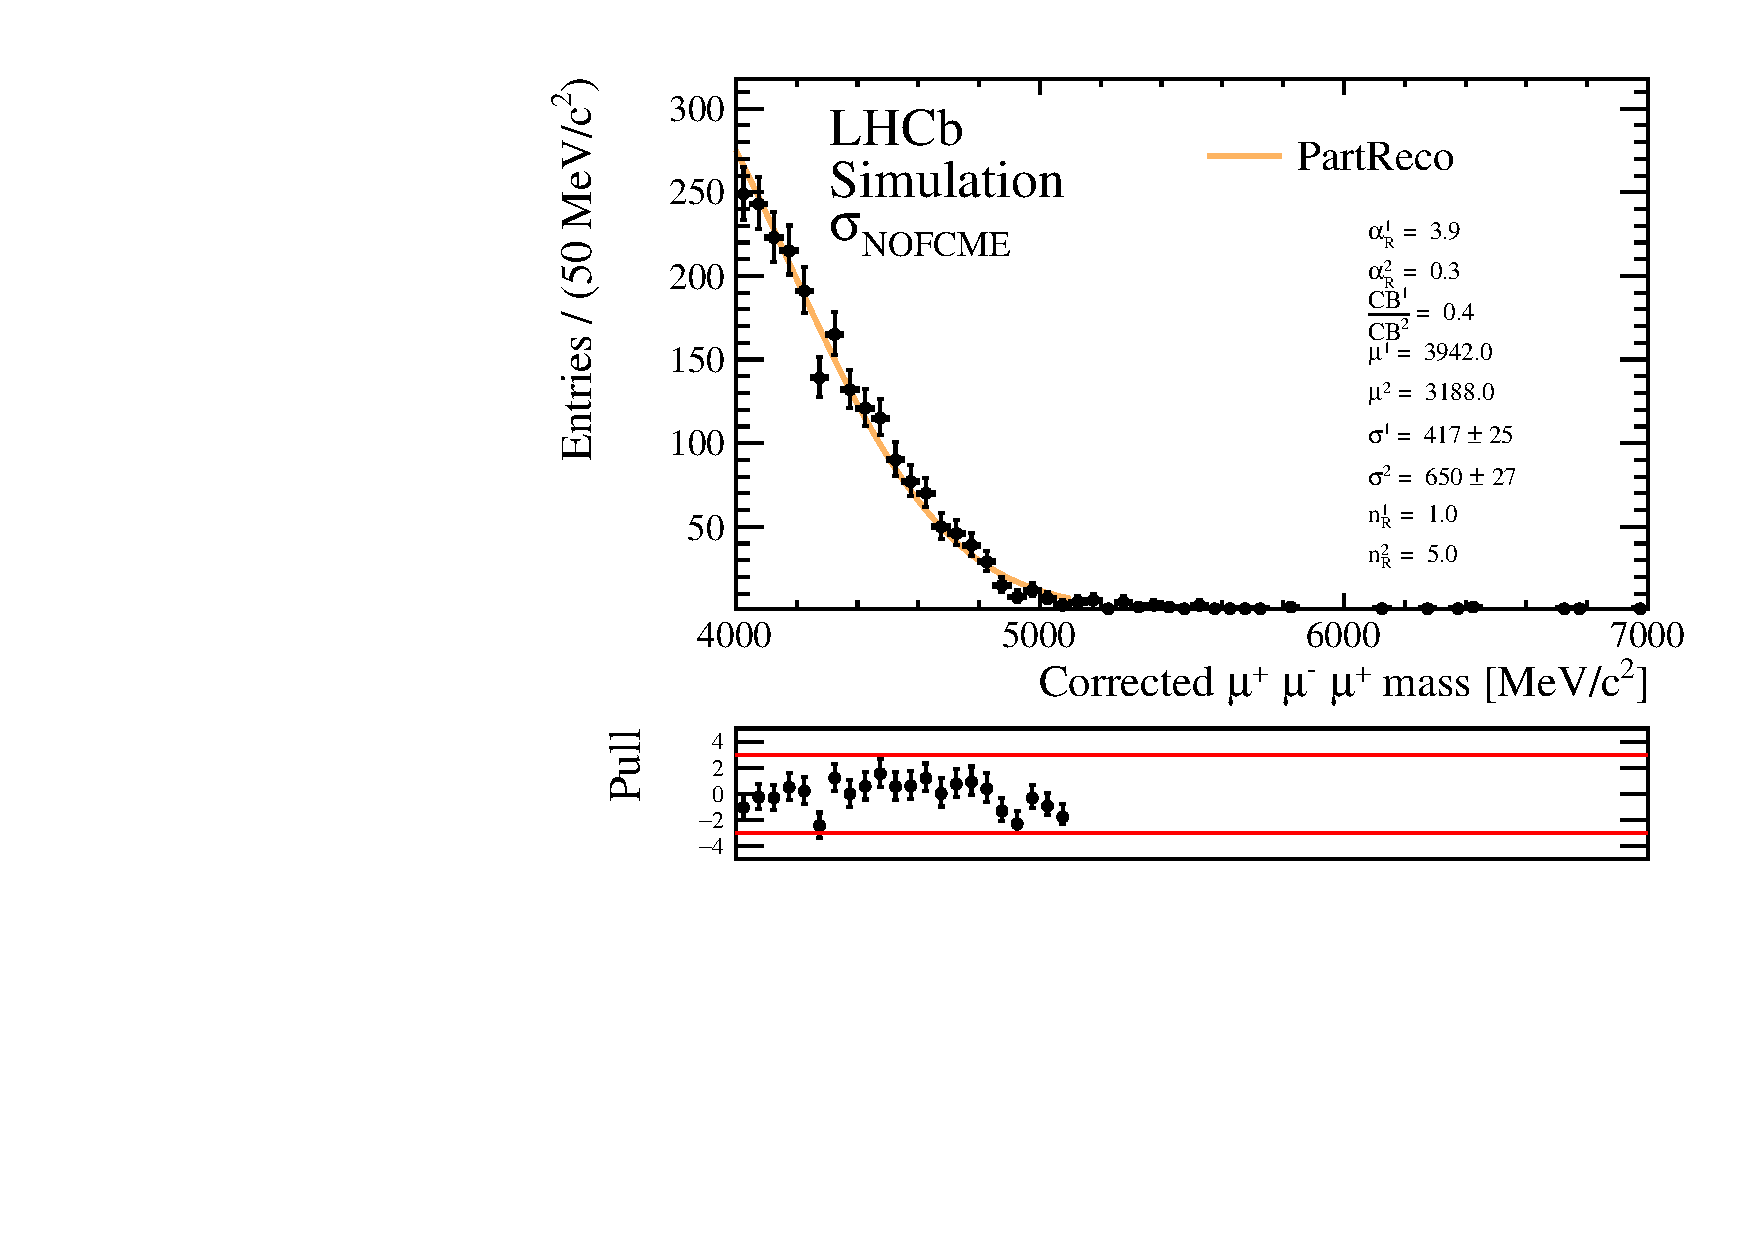
\includegraphics[width=0.5\linewidth]{./efficiency/signalfits/partrecomc/simprnofcmeRun1nolog.pdf}\put(-30,60){(a)}
%\newline
%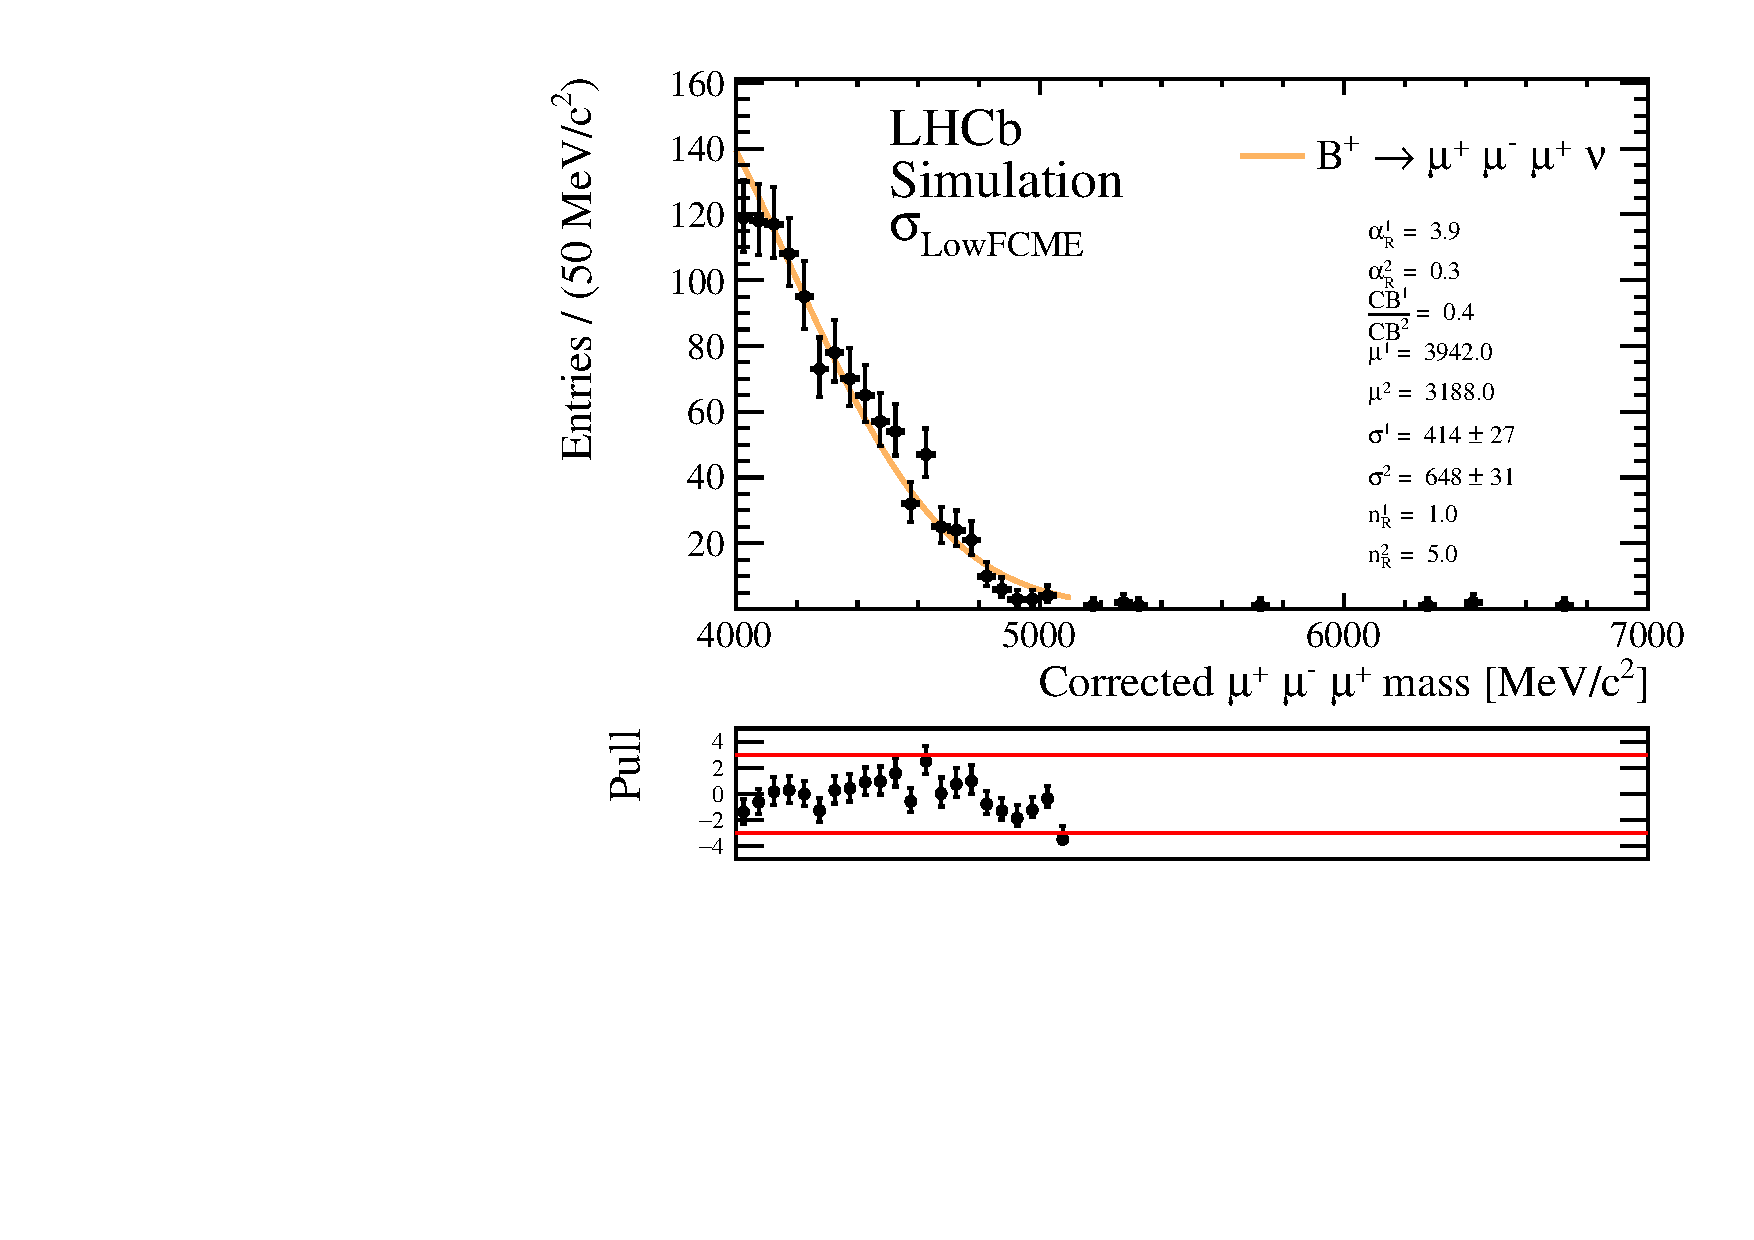
\includegraphics[width=0.5\linewidth]{./efficiency/signalfits/partrecomc/simprlowfcmeRun1nolog.pdf}\put(-30,60){(b)}%
%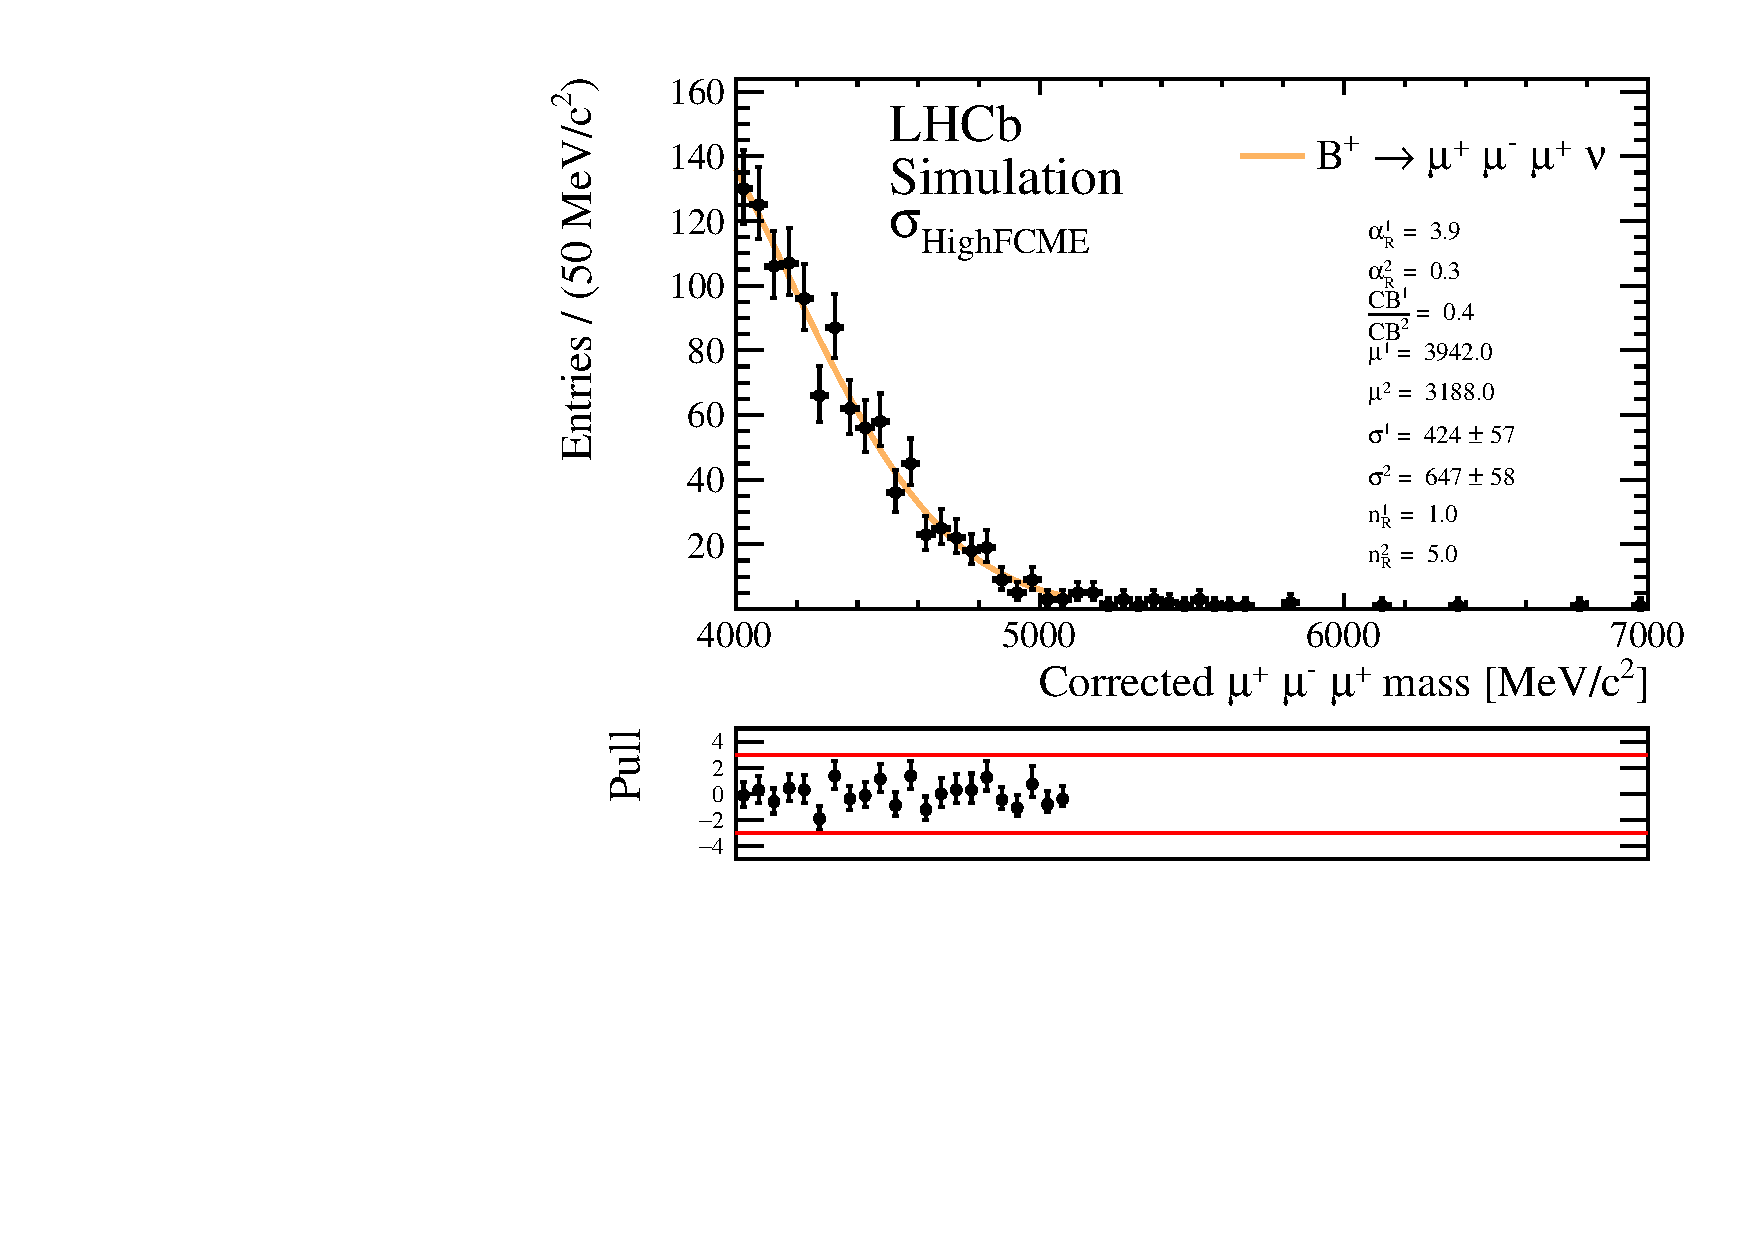
\includegraphics[width=0.5\linewidth]{./efficiency/signalfits/partrecomc/simprhighfcmeRun1nolog.pdf}\put(-30,60){(c)}%
%\caption{Fit to weighted combined partially reconstructed background simulation proxy for (a) NO FCME (b) Low FCME and (c) High FCME split.}
%%\vspace*{-1.0cm}
%\label{fig:PRFit}
%\end{figure}
%
%\subsubsection{MisID background}
%\label{misidfitstrat}
%The level and the shape of misID background is determined by fitting the misID data samples obtained using the method described in~\autoref{misidprocedure}. A binned $\chi^{2}$ fit is used to extract the shape and yields parameters. The reason for usage of the binned $\chi^{2}$ fit is that the misID samples are low-statistics weighted samples and the shape and yield needs be propagated to the final data fit while preserving the fit parameter correlations. Since there is prescale factor of 1\% at stripping level, to obtain the correct yield, the final number needs to be multiplied by to counteract the prescale.
%
%The misID weights obtained from kinematically binned \bjpsikst samples (see ~\autoref{extraction}) have uncertainties associated with them as shown in ~\autoref{fig:JpsiKnew},~\autoref{fig:JpsiKaonnew},~\autoref{fig:JpsiPionnew2016},~\autoref{fig:JpsiKaonnew2016}. These uncertainties are accounted for in the fit by Gaussian variation of the weights within the uncertainty in a given kinematic bin of $p,\eta$ for each particle species and then folded in to the misID calculation. In this case 100 variations were used. Each variation results in different template for misID shape. This misID template is then subsequently binned in 15 bins of corrected mass. From each corrected mass bin, mean $\mu_{var}$ and error $\sigma_{var}$ from gaussianly distributed number of misID events is obtained. 
%
%The total uncertainty due to the weight, $\sigma_{tot}$, for given bin of corrected mass is calculated using $\sqrt{\sigma_{var}^2 +\sqrt{\sum{w^{2}_{i}}}^{2}}$, where $\sigma_{par}=\sqrt{\sum{w^{2}_{i}}}$ is the associated error per bin and $\sigma_{var}$ is the standard deviation obtained from variation of misID weights. Finally, The binned $\chi^{2}$ fit is made to the misID samples with the total uncertainty. \textbf{The number of misID events}, $N^{MisID}$, for different species-regions after all selections are seen in~\autoref{tab:misidtabcummu}. Hence for non-simultaneous fit this just add 1 parameter and for simultaneous fit there will be two parameters describing the total yield of misID.
%
%Also it can be seen in~\autoref{tab:misidtabcummu}, crossfeedweight is only considered for kaon-like and pion-like \textit{SS misID} samples. This arises as a consequence of two characteristics of the misID crossfeedweight procedure. First the convergence criteria makes unbalanced samples (one sample very high in misID events and other sample very small in number of misID events) hard to satisfy (case for most of \textit{OS misID} samples). Secondly, proton-like region samples are very sparse and hence it is not necessary to account for crossfeed. %, see Figure ~\ref{fig:ProtonPIDHeatMap}.
%
%The binned $\chi^{2}$ fits using Crystal Ball function to different bins of FCME is performed as seen in~\autoref{fig:MisidFinalFit}. This means that \textbf{the shape} of this background, $f^{MisID}$, is a function of 4 parameters in non-simultaneous case and a function of 8 parameters in simultaneous case. Both full weight error $\sigma_{tot}$ and partial weight error $\sigma_{par}$ are plotted. The difference between the two is the error due to uncertainty on the weight $\sigma_{var}$.  Results of the fits are propagated into the signal data fits preserving correlations between parameters, which are hence set as multidimensional gaussian constraints in the signal data fits. This means that all uncertainties due to misID will be directly accounted for in the signal data fits.
%
%
%\begin{table}[H]
%\small
%\begin{center}
%\begin{tabular}{ l  l  l  l  l  }
%\toprule
%Sample & Region & PID & weight & Cummulative  \\
% &  &  &  & misID count \\
%\midrule
%Run \Rn{1} \textit{SS misID} & Kaon-region & Run \Rn{1} PID & crossfeedweight & 198 \\
%Run \Rn{1} \textit{SS misID} & Pion-region  &  & crossfeedweight & 301 \\
%Run \Rn{1} \textit{SS misID} & Proton-region &  & no-crossfeedweight & 307 \\
%Run \Rn{1} \textit{OS misID} & Kaon-region &  & no-crossfeedweight & 310 \\
%Run \Rn{1} \textit{OS misID} & Pion-region &  & no-crossfeedweight & 352 \\
%Run \Rn{1} \textit{OS misID} & Proton-region &  & no-crossfeedweight & 353 \\
%Run \Rn{2} \textit{SS misID} & Kaon-region & Run \Rn{2} PID  & crossfeedweight & 489 \\
%Run \Rn{2} \textit{SS misID} & Pion-region &  & crossfeedweight & 565 \\
%Run \Rn{2} \textit{SS misID} & Proton-region &  & no-crossfeedweight & 565 \\
%Run \Rn{2} \textit{OS misID} & Kaon-region &  & no-crossfeedweight & 573 \\
%Run \Rn{2} \textit{OS misID} & Pion-region &  & no-crossfeedweight & 618 \\
%Run \Rn{2} \textit{OS misID} & Proton-region &  & no-crossfeedweight & 619 \\
%\bottomrule
%\end{tabular}
%\end{center}
%	\caption{The final misid template is constructed by summing the contribution from Run \Rn{1} and \Rn{2} kaon, pion and proton-like regions for both \textit{SS} and \textit{OS misID} contributions. The last column adds cummulatively the contributions with respect to the previous row. }
%\label{tab:misidtabcummu}
%\end{table}
%
%\begin{figure}[H]
%\centering
%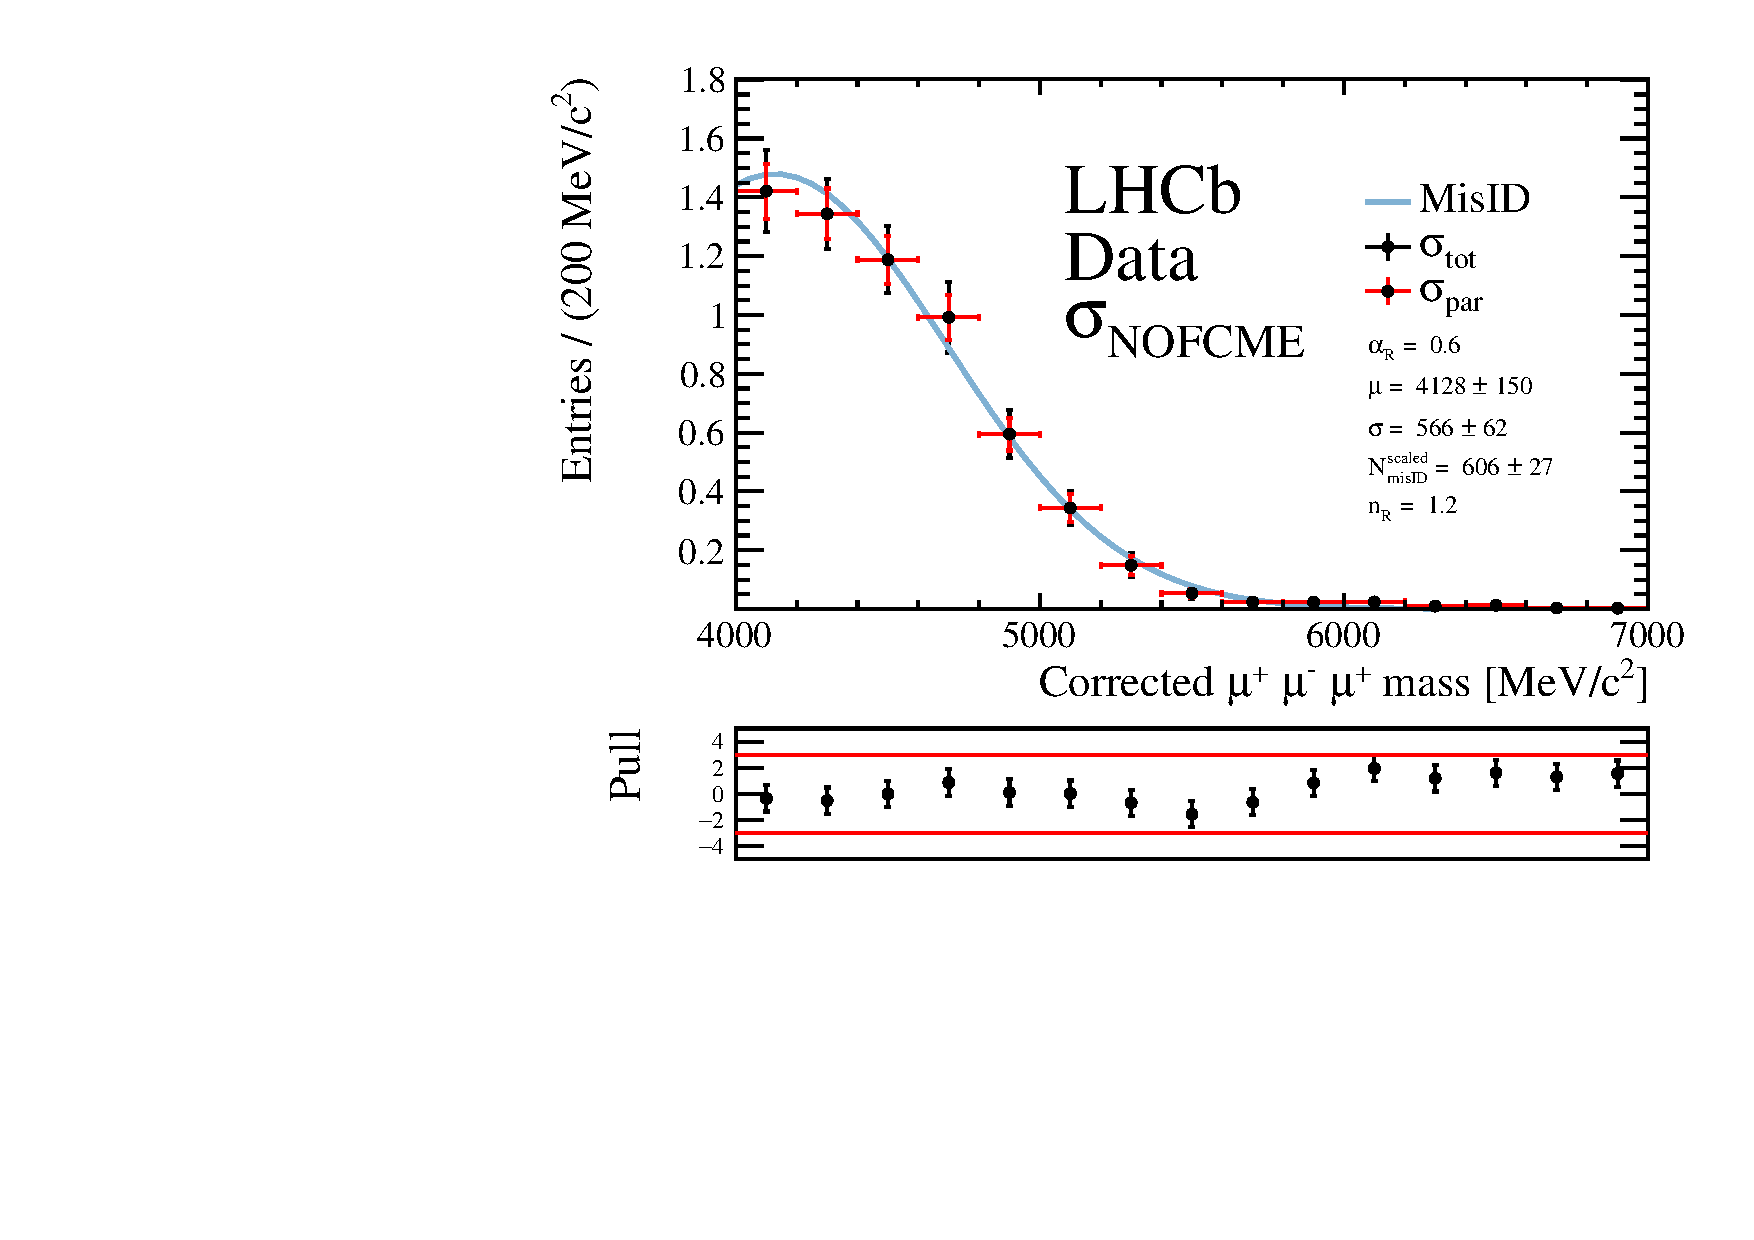
\includegraphics[width=0.5\linewidth]{./efficiency/signalfits/misiddata/misiddatanofcmeRun1nolog.pdf}\put(-30,60){(a)}
%\newline
%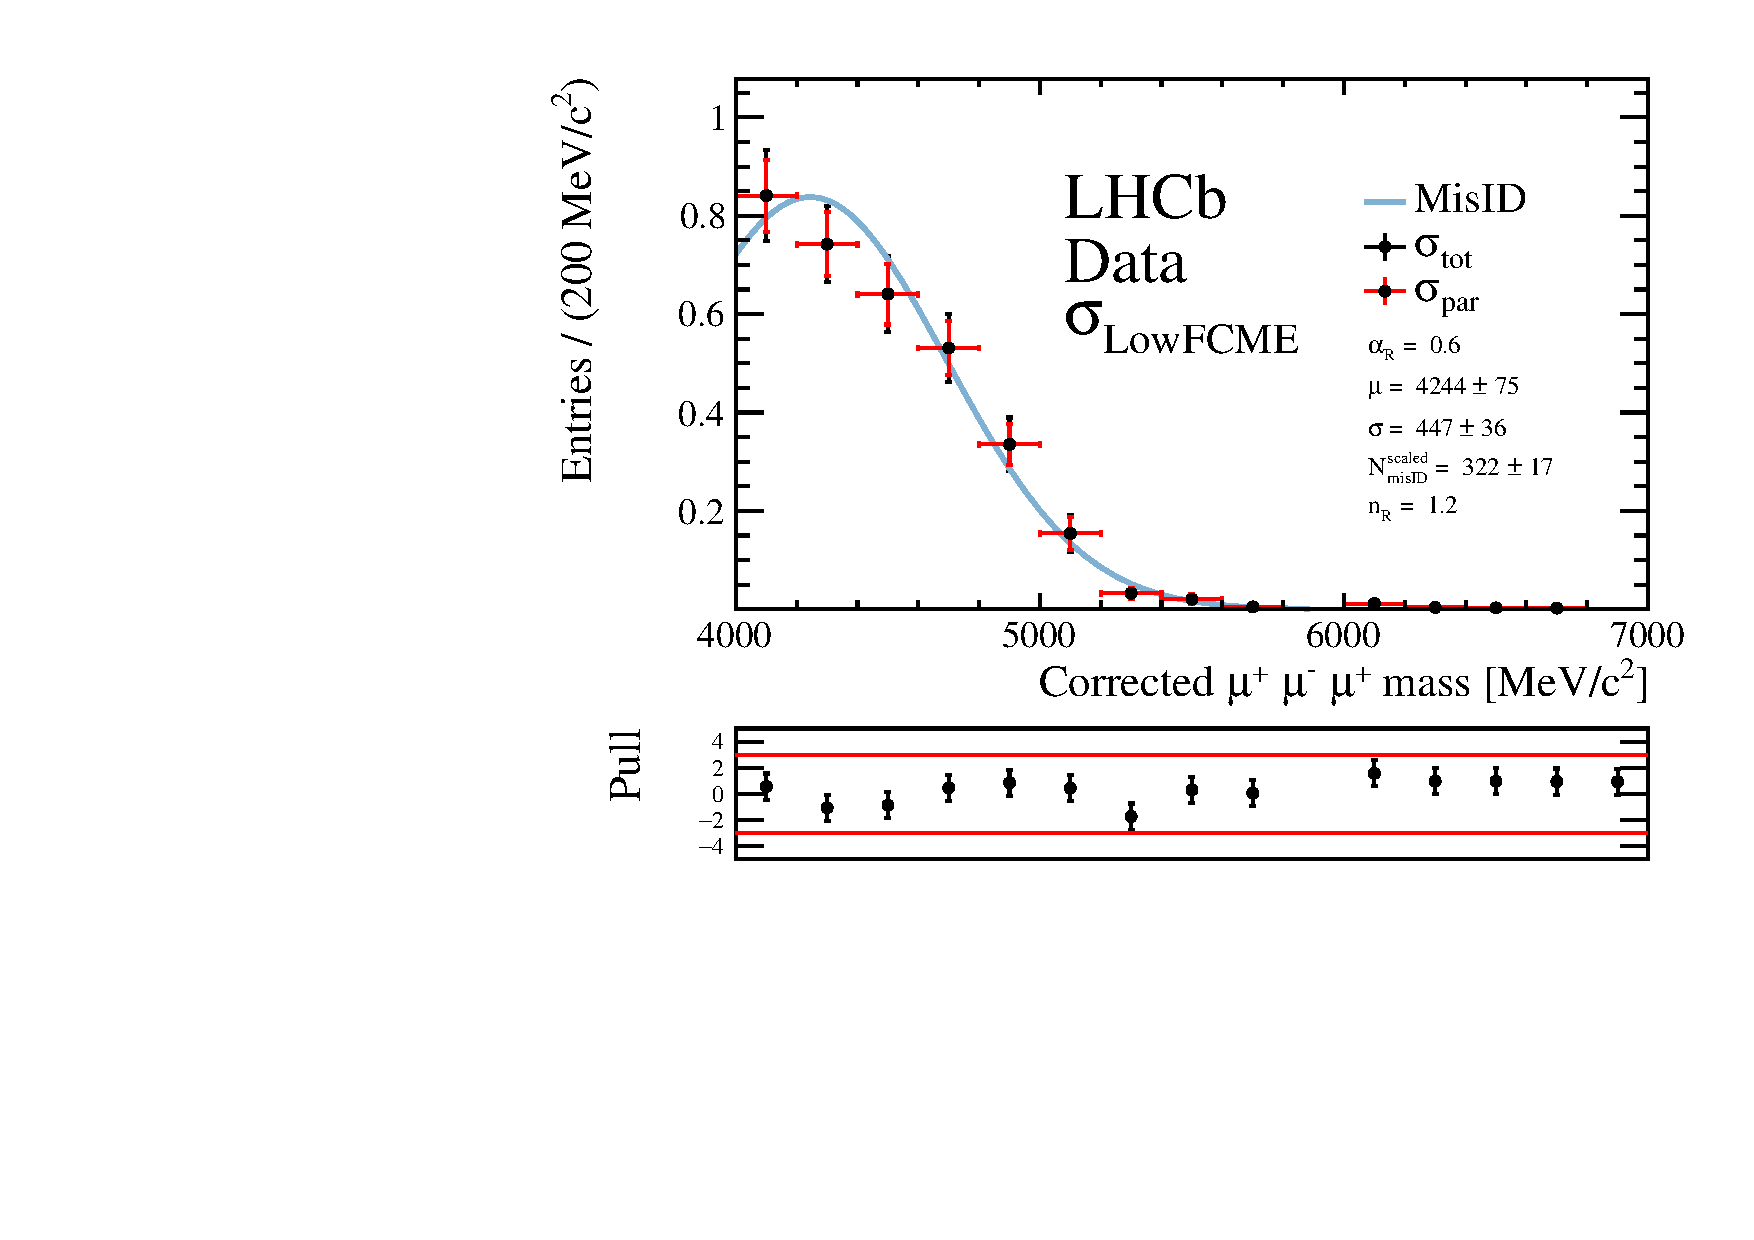
\includegraphics[width=0.5\linewidth]{./efficiency/signalfits/misiddata/misiddatalowfcmeRun1nolog.pdf}\put(-30,60){(b)}%
%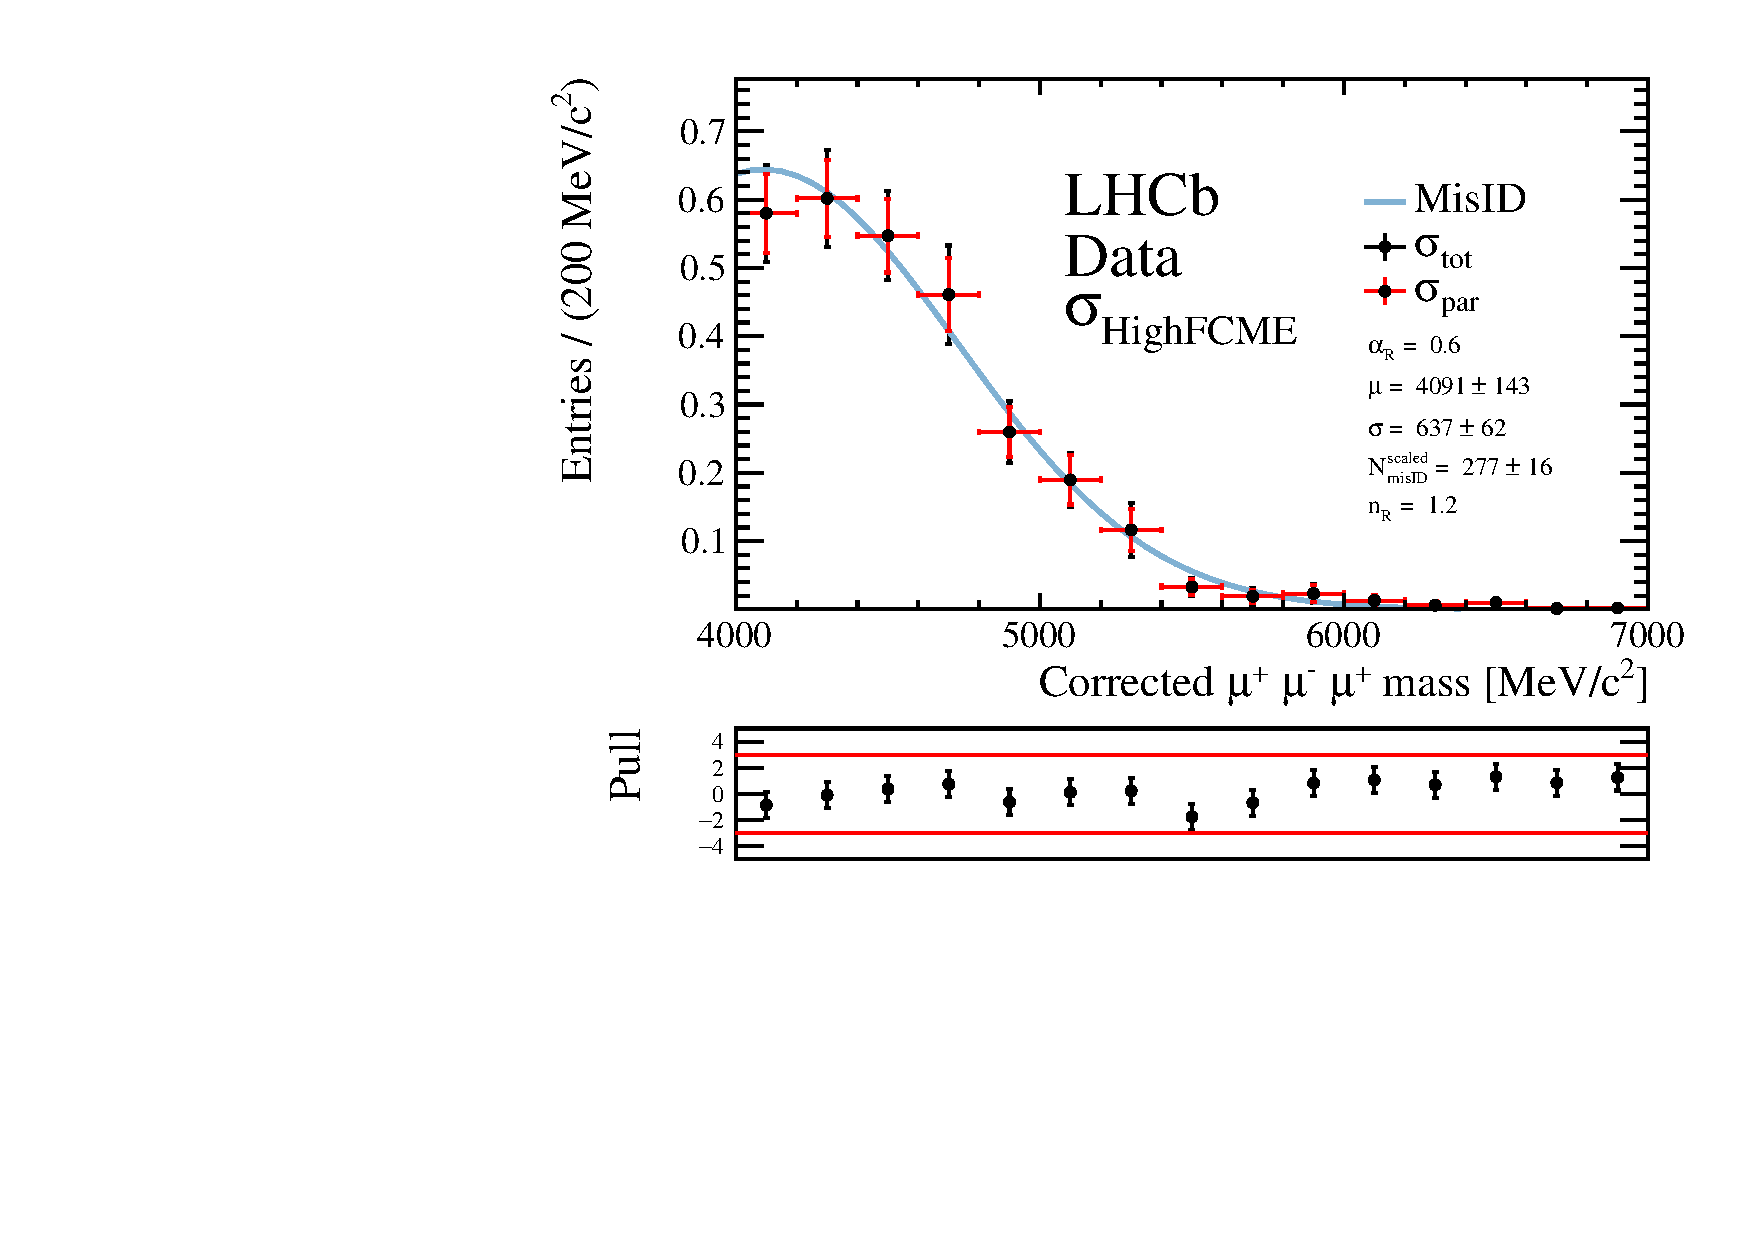
\includegraphics[width=0.5\linewidth]{./efficiency/signalfits/misiddata/misiddatahighfcmeRun1nolog.pdf}\put(-30,60){(c)}%
%	\caption{Binned $\chi^{2}$ to misid template with no FCME split (b) Low FCME (c) High FCME. In high FCME bin, the distibution of misid is pollutes signal window more than in the low FCME bin. Both full weight error $\sigma_{tot}$ and partial weight error $\sigma_{par}$ can be seen.}
%%\vspace*{-1.0cm}
%\label{fig:MisidFinalFit}
%\end{figure}
%
%\subsubsection{Combinatorial Background}
%Signal data fit so far includes components for signal component, partially reconstructed background component, and misid background component. The only component left to estimate is the contamination of combinatorial background. To model the combinatorial component exponential function is left floating and fit to data, which was motivated in~\autoref{combiback}. Hence \textbf{the shape}, $f^{Combi}$, has one(two) parameter(s) for non-simultaneous(simultaneous) fit, which is the exponential constant. And \textbf{the yield}, $N^{Combi}$, is also parametrised just with one (two) parameter(s) for non-simultaneous (simultaneous) fit.
%
\subsection{Signal Data Fits}
\label{fitsens}


\subsubsection{Signal fit models}
The full signal fit model consists of all the mentioned components. As mentioned in~\autoref{sigpara} there are two fit models that are used to fit data: non-simultaneous, $f^{NS}(x,y^{i})$, and simultaneous fit model, $f^{S}(x,{z^{k}})$, where the latter is the one which is used for the limit setting. In this case $x$ is the corrected mass, and $y^{i}(z^{k})$ are all the parameters for the non-simultaneous (simultaneous) fit. The total fit models hence can be written 
\begin{equation}
f^{NS}(x,y^{i})=N^{sig}\times f^{sig} + N^{MisID}f^{MisID} + N^{PR}f^{PR} + N^{Combi} \times f^{Combi},
\label{eq:fullhypo}
\end{equation}

\begin{equation}
f^{S}(x,y^{k})=\sum_{j\in{\sigma}}(N_{j}^{sig}\times f_{j}^{sig} + N_{j}^{MisID}f_{j}^{MisID} + N_{j}^{PartReco}f_{j}^{PartReco} + N_{j}^{Combi} \times f_{j}^{Combi}),
\label{eq:fullhypo2}
\end{equation}
where $\sigma$ is the bin of fractional corrected mass. The shared parameters in the two bins of fractional corrected mass error for the simultaneous fit are the branching fractions $\mathcal{B}(\Bmumumu),\mathcal{B}(\pr),\mathcal{B}(\bjpsimumuk)$. 
%non sim 30 param.
%sim 56 param.

\subsubsection{Signal fit model hypotheses}
As the strength of the signal is not a priori known, there are two types of hypotheses that are established: one where there is a presence of signal, also known as signal+background hypothesis model which takes exactly form of~\autoref{eq:fullhypo} and then a background only hypothesis, where $\mathcal{B}(\Bmumumu)=0 \rightarrow N^{sig}=0$.

\subsubsection{Signal data types}

There are two types of signal datasets as mentioned in~\autoref{Strategy}. Firstly, there is \textbf{blinded signal data} to which the simultaneous and non-simultaneous fits are performed in order to evaluate the expected sensitivity. Since these datasets are blinded only the mass regions $4000{\mevcc}<M_{\rm{B_{corr}}}<{4500\mevcc}$ and $5500{\mevcc}<M_{\rm{B_{corr}}}<{7000\mevcc}$ are used in the fits. These fits are shown in~\autoref{blindeddatafit}. Secondly fits to \textbf{full signal data} are performed and these are used in order to set the limit on the $\mathcal{B}(\Bmumumu)$. In these fits the full mass spectrum is used.

\subsection{Signal Fit Systematics}
\label{systematics}
Systematics studies are performed in order to account for possible shortcomings of the methods used in order to measure $\mathcal{B}(\Bmumumu)$. The summary of systematic uncertainties is provided in~\autoref{tab:systematicsummary}. Most of this systematic uncertainties directly affect the efficiency ratio between signal and normalisation channel. In that case, fits account for this uncertainty directly by incorporating the uncertainty into efficiency ratios by adding them in quadrature to the statistical error. For the simultaneous fit these uncertainties are assumed to be $100\%$ correlated between the bins of FCME.


\begin{table}[H]
\centering
%\small
\begin{tabular}{ l  c  c  c  }
\toprule
Systematic source & Run \Rn{1}/\% &  Run \Rn{2}/\% & Error Overall \\ \hline

$\mathcal{B}(J/\psi \rightarrow \mu^{+} \mu^{-})$ & 0.6 & 0.6 & 0.6\\
$\mathcal{B}(B^{+} \rightarrow  J/\psi K^{+})$ & 3.0 & 3.0 & 3.0\\
\hline
Signal Decay Model & 4.6 & 4.6 & 4.6\\
Trigger Data/Sim & 5.1 & 1.3& 3.2\\
Trigger \texttt{HLT2} &  -  &  1.5& 1.5\\
Kaon interaction probability &  2.0  &  2.0& 2.0\\
Kinematic Reweighting & 1.0 & 2.0 &1.5\\
Simulation Statistics & 1.3 & 0.7 & 0.8 \\
Fit bias & 1.0 & 1.0 & 1.0  \\
 \hline
 Total & 8.0 & 6.6 & \textbf{7.1} \\
 \hline
Statistical source & Run 1/\% & 2016/\% & Error Overall \\ \hline
Error on $B^{+} \rightarrow J/\psi K^{+}$ yield & 0.3 & 0.3 & 0.2\\
 \bottomrule
\end{tabular}
\caption{Summary of systematic uncertainties.}
\label{tab:systematicsummary}
\end{table}




\subsubsection{Signal Decay Model}
The largest systematic uncertainty arise due to the choice of decay model for the signal channel.
The nominal signal model creates a photon pole, increasing the branching fraction in the low invariant dimuon mass region.
The associated systematic uncertainty is estimated by replacing this decay model with one determined purely by phase-space and by comparing the selection efficiencies, resulting in $4.6\%$ systematic uncertainty on the efficiency ratio. % In the data fits this uncertainty directly incorporated into efficiency ratios, $R_{\mathrm{FCME}}$, by adding it in quadrature to the statistical error. 

\subsubsection{Trigger}
The second most important systematic effect is due to incorrect modelling of the trigger in the simulation. This can be split into two effects:
 the efficiency difference between used simulation and data and incorrect emulation of \texttt{HLT2} in the simulation in 2016 as only one \texttt{TCK} was considered for this trigger selection. This uncertainty is assigned by comparing the difference between the trigger efficiency of \bjpsimumuk decays in simulation and data using the \texttt{TISTOS method}.

The \texttt{TISTOS method} allows measuring the trigger efficiency, whereby the events that are \gls{TIS} and \gls{TOS} are assumed to be independent. Hence, the efficiency
for selection of \gls{TOS} candidates can be calculated by

\begin{equation}
\varepsilon_{TOS} = \frac{N_{TIS\&TOS}}{N_{TIS}}.
\label{eq:tistos}
\end{equation}
In~\autoref{eq:tistos} $N_{TIS\&TOS}$ is the number of \gls{TIS} and \gls{TOS} events passing the trigger requirement and $N_{TIS}$ is the number of \gls{TIS} events which passed the trigger requirement.

The efficiency difference of the full trigger chain between \bjpsik decays in used simulation and \textit{Sweighted} data is $3.2\%$. Incorrect emulation of \texttt{HLT2}, which is calculated by comparing \texttt{HLT2} trigger efficiency of the chosen TCK simulation and all the \textit{Sweighted} data, yields $1.5\%$. Altogether the incorrect modelling of the trigger in simulation results in a $3.5\%$ systematic uncertainty.

\subsubsection{Kaon Interaction Probability}
One difference between the signal and the normalisation channels that can have effect on the efficiencies is that the kaon in the decay \bjpsimumuk can interact with the detector at a probability proportional to the amount of material traversed. The uncertainty on this amount of material leads to a 2\% systematic
uncertainty, which follows the procedure outlined in Ref.~\cite{LHCb-DP-2013-002}.

\subsubsection{Kinematic Reweighting}
Another source of systematic uncertainty is caused by differences in the $B^{+}$ production kinematics in the simulation. Corrected variables are momentum, $p$, transverse momentum $p_{T}$ and vertex $\chi^{2}$ of $B$. The kinematic weights in a given kinematic bin are calculated using normalised histograms of \bjpsimumuk data, and normalized \bjpsimumuk simulation in a following way
\begin{equation}
w_{(bin)} =  \frac{w_{\bjpsimumuk data,bin}}{w_{\bjpsimumuk simulation,bin}}.
\end{equation}
Obtained correction weights are then applied to correct both the \bjpsimumuk and \Bmumumu simulation. The difference between uncorrected and kinematically corrected efficiency ratios is assigned as a systematic uncertainty yielding $1.5\%$ systematic uncertainty on the efficiency ratios.

\subsubsection{Signal Fit Bias and Coverage}
In this section systematic uncertainty due to signal bias is evaluated. The pull is calculated using pseudo-experiments where the data is generated for signal branching fraction $\mathcal{B}= 1.0\times 10^{-8}$ corresponding to $\approx$ 17 signal events for Run \Rn{1} and \Rn{2} data.
These pseudo-datasets are then re-fitted with floating $\mathcal{B}$ and corresponding number of fitted signal events is obtained. The pull is defined as the difference between number of fitted signal events and the number events that pseudo-experiment was created with, divided by the error on the number of signal events given by the fit:
\begin{equation}
\frac{N^{orig}_{sig}-N^{fit}_{sig}}{\sigma^{fit}}.
\end{equation}

The pull distributions can be fitted with a gaussian function and the fit bias is calculated as a shift of the mean from 0. The overcoverage/undecoverage of the fit is established by shift of the standard deviation of the gaussian function from 1.

For this study 10000 pseudo-experiments were created testing the bias and coverage of both the extended non-simultaneous fit and extended simultaneous fit. The pull distributions for the non-simultaneous fit can be seen in ~\autoref{fig:SignalBias}.
\begin{figure}[H]
\centering
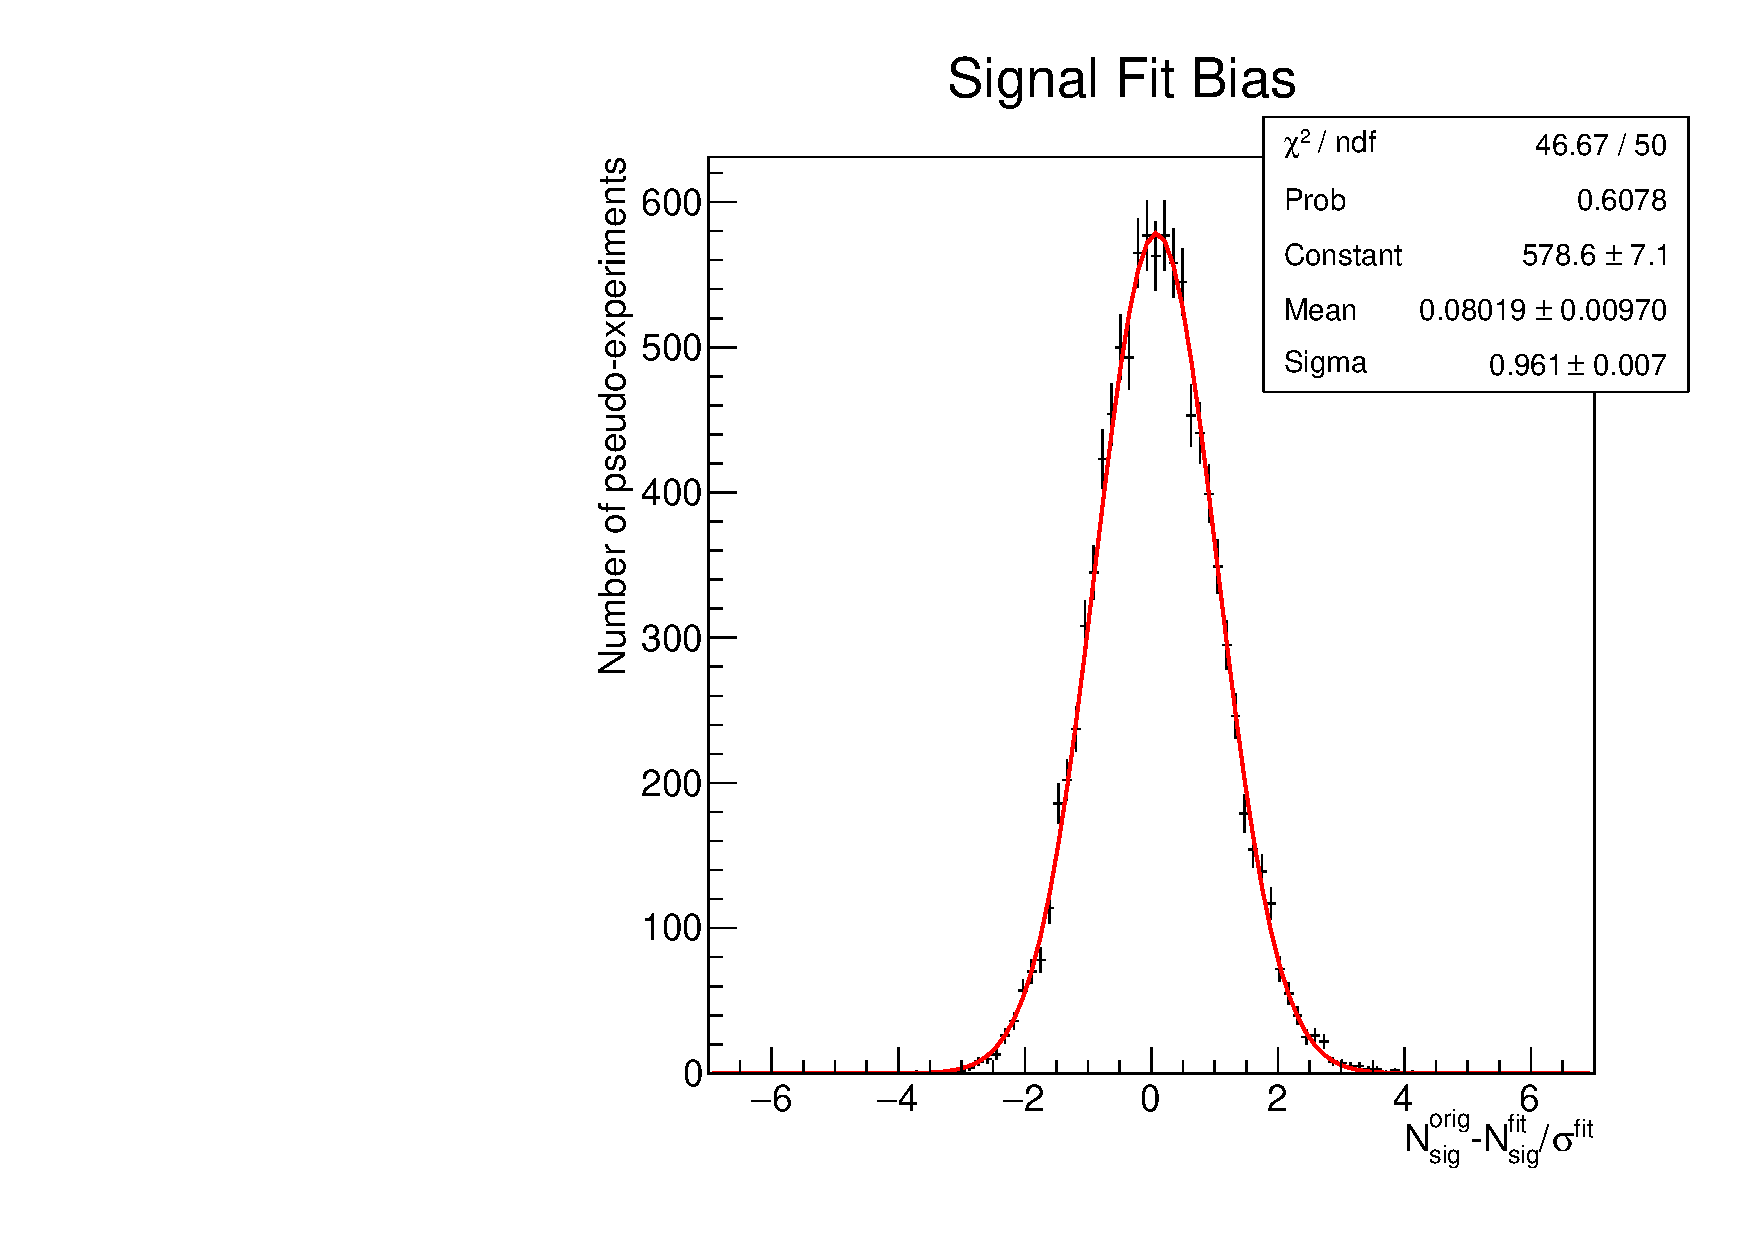
\includegraphics[width=0.5\linewidth]{./efficiency/systematics/signalbias/notsim.pdf}
%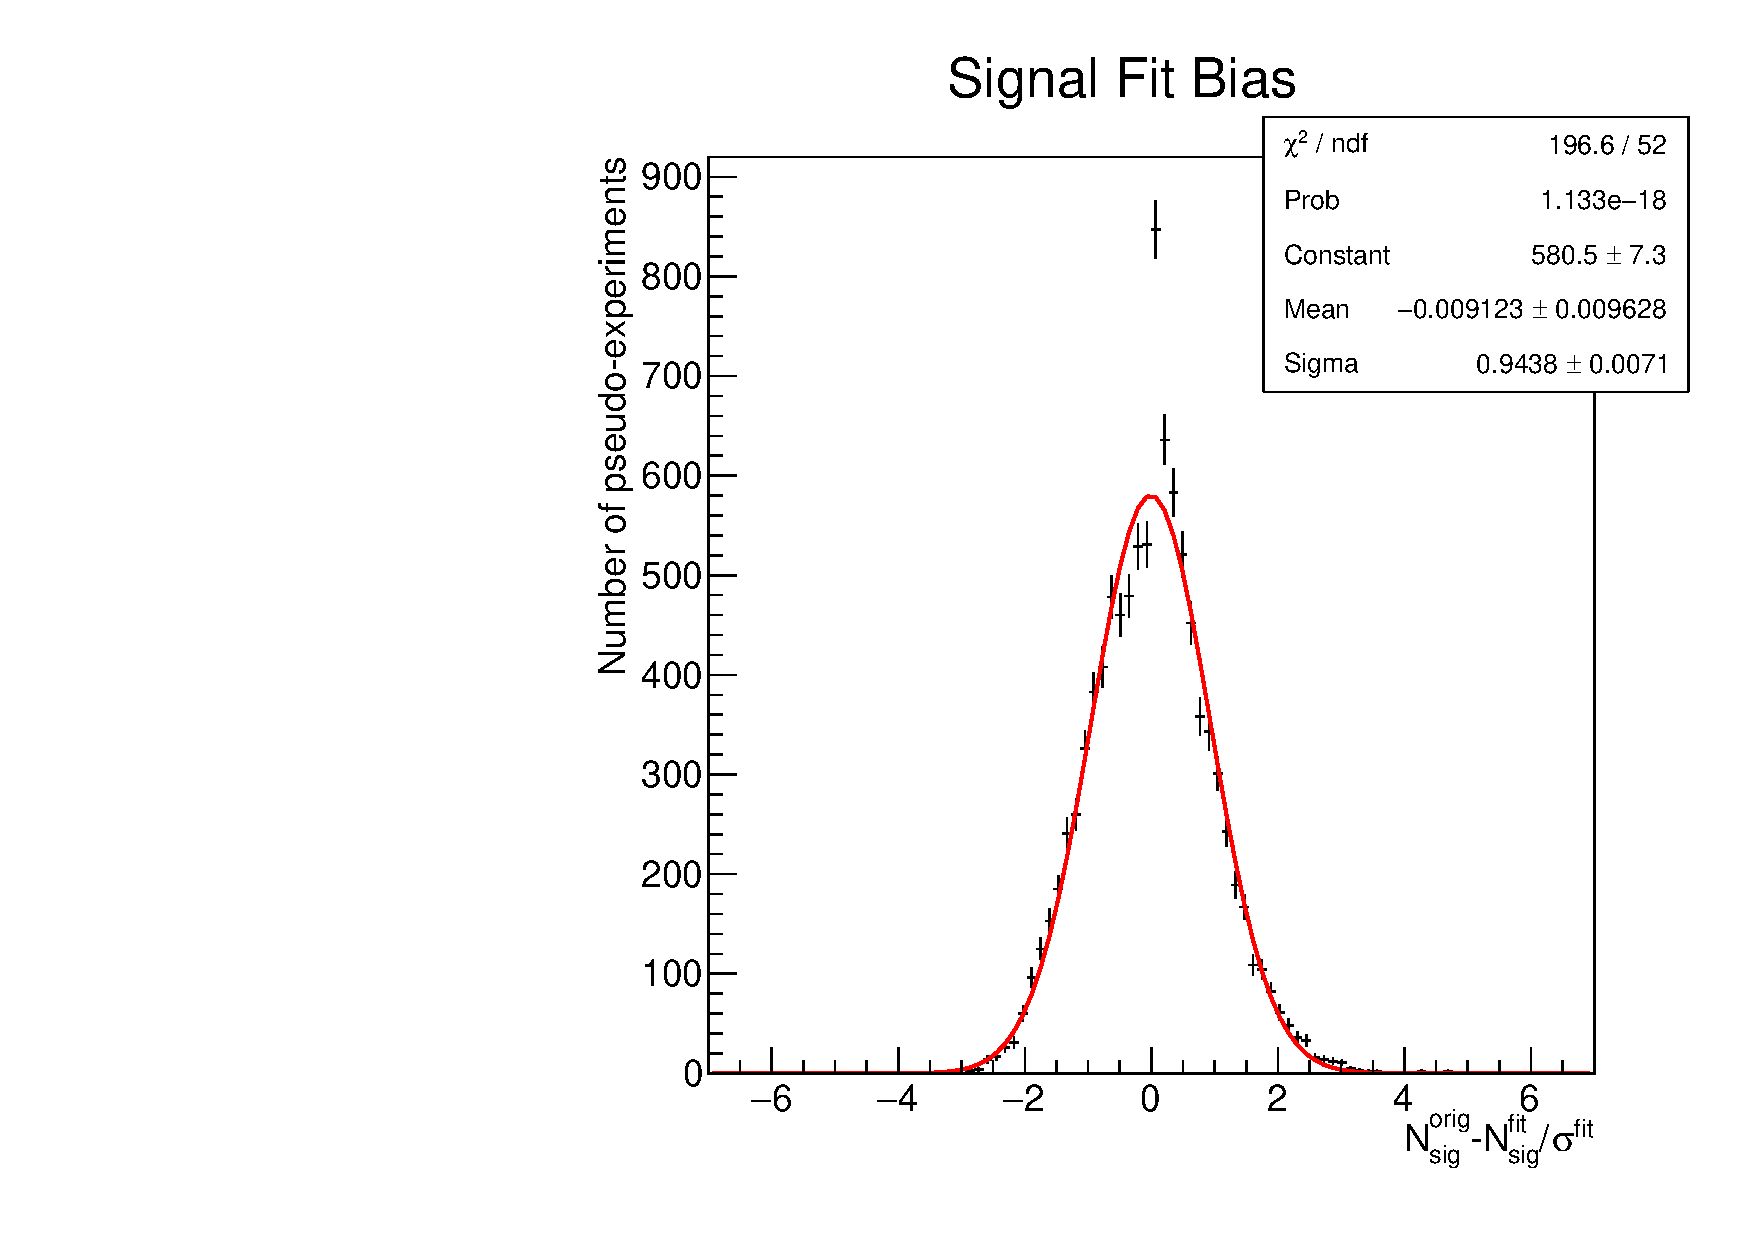
\includegraphics[width=0.5\linewidth]{./efficiency/systematics/signalbias/sim.pdf}\put(-50,60){(b)}
%\newline
%\includegraphics[width=0.5\linewidth]{./systematics/signalbias/SignalError_signal_numoftoys_10000_injectsig1e-08.pdf}\put(-50,60){(c)}
\caption{Non-simultaneous fit pulls from 10000 pseudo-experiments.}
%\vspace*{-1.0cm}
%\caption{(a) Non-simultaneous fit, (b) simultaneous fit pulls.}
\label{fig:SignalBias}
\end{figure}

As it can be seen, for non-simultaneous fit there is overcoverage of 4 $\%$ but since the statistical error is of the order of 100$\%$ this is insignificant.
The bias shows 8$\%$ preference for lower signal yields, and hence this will be added as a systematic uncertainty. The same process was repeated for simultaneous fit and results can be seen in~\autoref{tab:biassum}. 

\begin{table}[H]
\begin{center}
\begin{tabular}{ l  l  l  l  l }
\toprule
        Fit & $\mathcal{B}$ & Statistical Error & Overcoverage & Bias \\
\hline
        Not Simultaneous  & $1.0\times 10^{-8}$ & $\approx$ 100\% & 4\% & 8\%   \\
        Simultaneous  & $1.0\times 10^{-8}$ & $\approx$ 100\% & 6\% & 1\%   \\
\bottomrule
\end{tabular}
\end{center}
\caption{Signal bias estimate from 10 000 pseudo-experiments for both simultaneous and not simultaneous fit.}
\label{tab:biassum}
\end{table}


\subsubsection{Others}
Other smaller systematic uncertainties are assigned due to the finite size of the simulation and the branching fraction of the decay $\jpsi \to \mumu$ and \bjpsik.



\subsection{Blinded Data Fits}
\label{blindeddatafit}
In order to be able to get the expected sensitivity for this search a simultaneous unbinned maximum likelihood extended fit to the blinded data of corrected mass after the full selection in two bins of FCME is performed. As a crosscheck, also the non-simultaneous fit with no FCME split is done. The summary of all the components adding to the total PDF for the blinded signal data fit, their modelling and constraints are shown in~\autoref{tab:floatingparsummary}.

Most of the parameters in these fits are fixed and if they are not fixed they are constrained with their range allowed to be within $\pm5\sigma$ of the constraint. Error propagation from the parametrisations of different components is dealt with by using two types of constraints: gaussian constraints and multivariate gaussian constraints. The gaussian constraint, \textit{gaussian}, when imposed has central value of the fitted parameter and as width the error of the fitted parameter. Multivariate gaussian constraint, \textit{mvg\_gaussian}, is generalisation of gaussian constraint to higher dimensions and is used for misID parametrisation as the correlations between different parameters need to be propagated to the signal fit.

The maximum unbinned likelihood fit to blinded signal data after all selection is shown in~\autoref{fig:sigfitpretty} for all categories of FCME. As the signal region is blinded in this case the fit model uses the background-only hypothesis. The total number of expected background events, $N_b$, can be then obtained by integrating the total PDF in the signal region.

\begin{figure}[H]
\centering
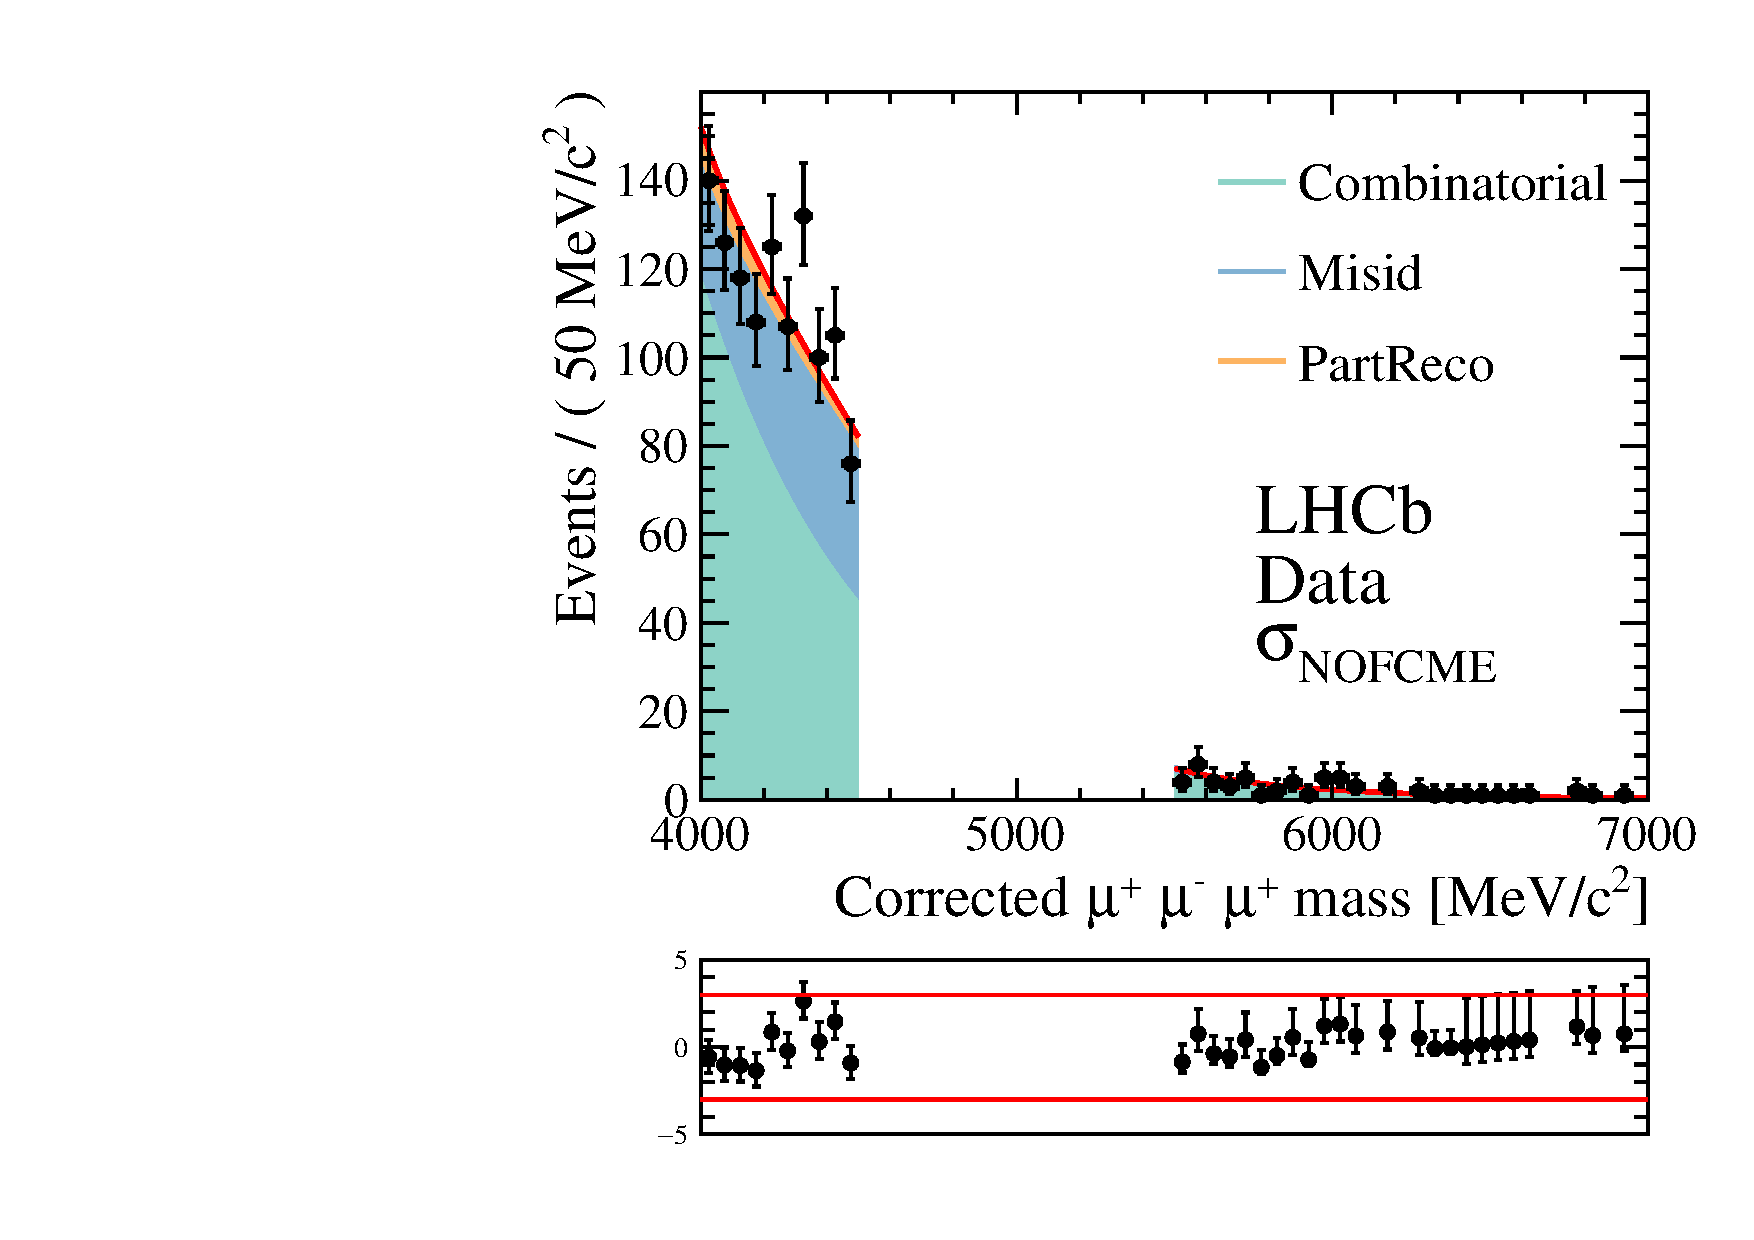
\includegraphics[width=0.5\linewidth]{./efficiency/blindedfits/probnnmu035probmu35plotB23MuNuFitPretty_chi2_reallynice.pdf}\put(-30,100){(a)}%
\newline
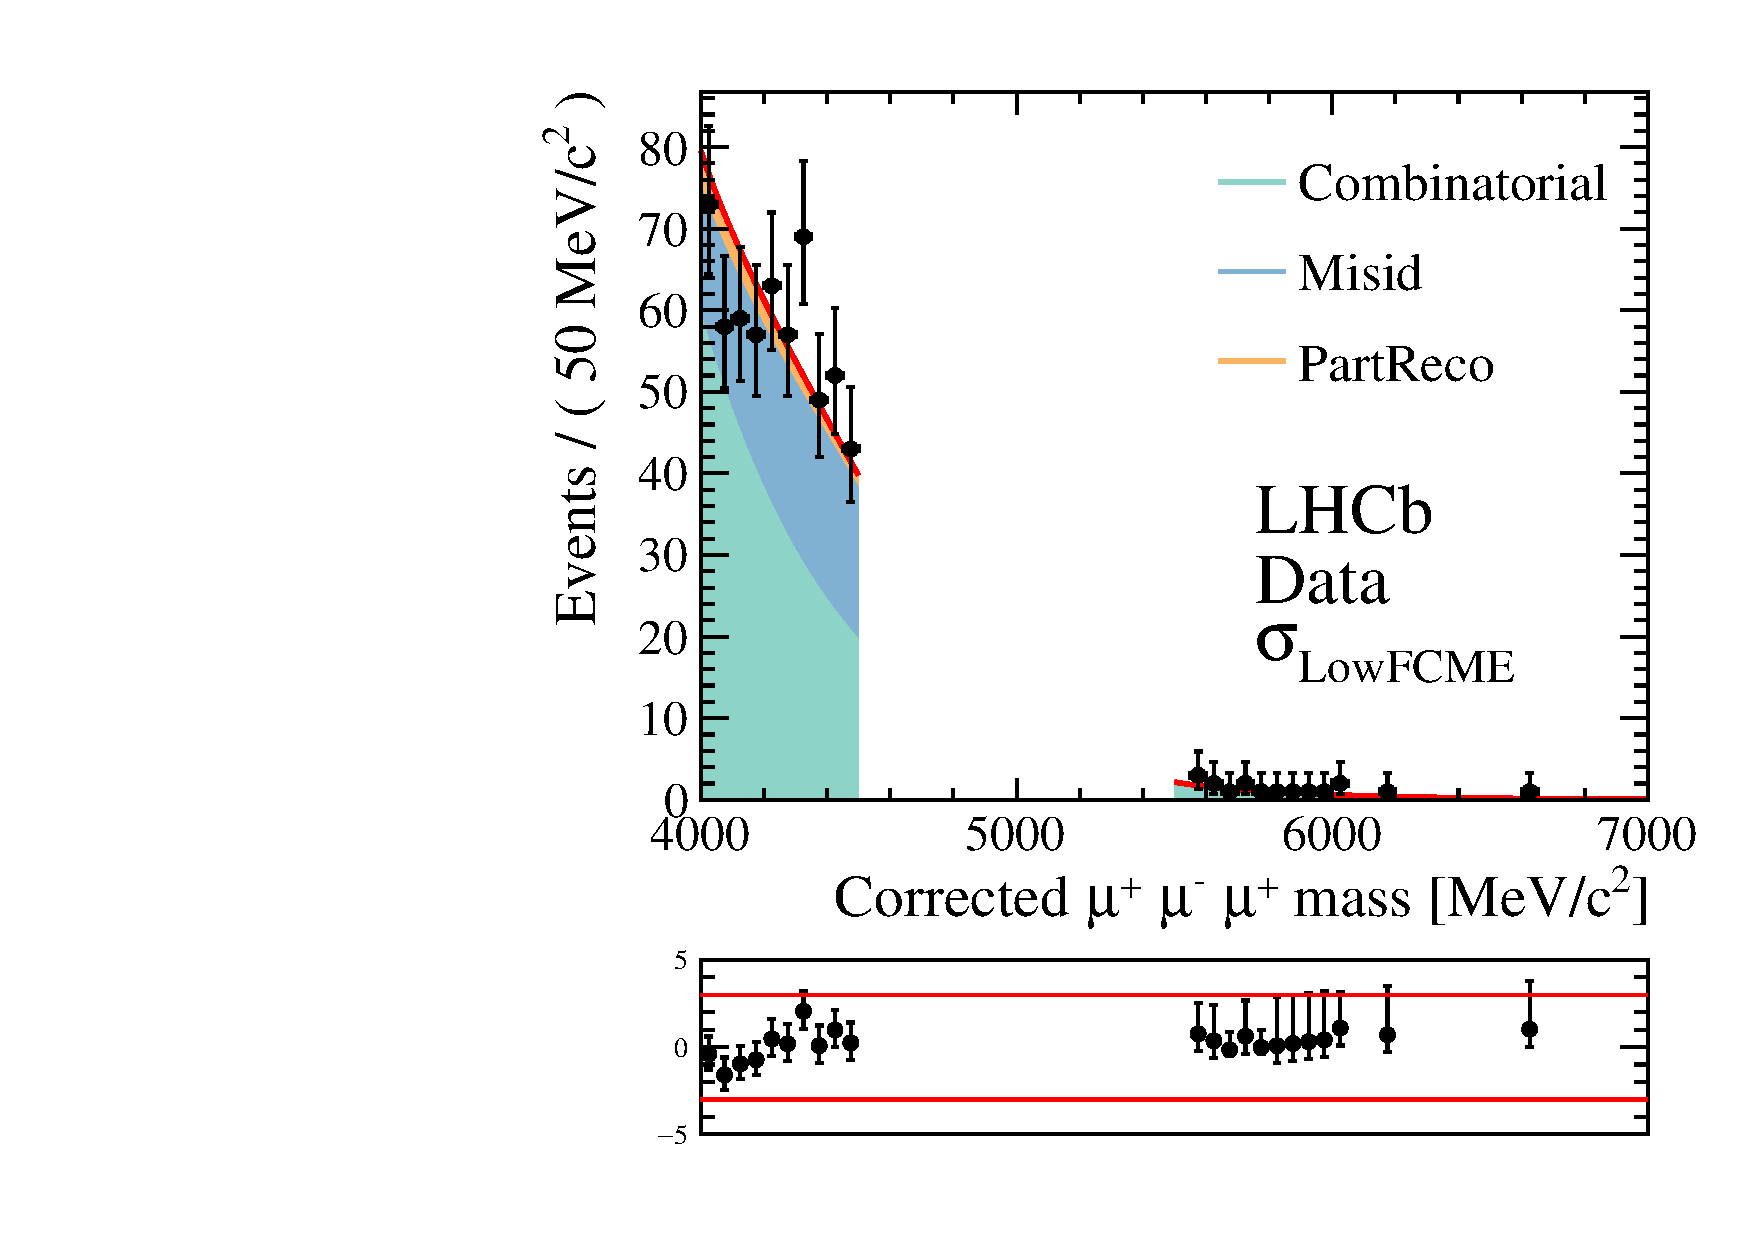
\includegraphics[width=0.5\linewidth]{./efficiency/blindedfits/LowFCMEprobnnmu035probmu35plotB23MuNuFitPretty_chi2_reallynice.pdf}\put(-30,100){(b)}%
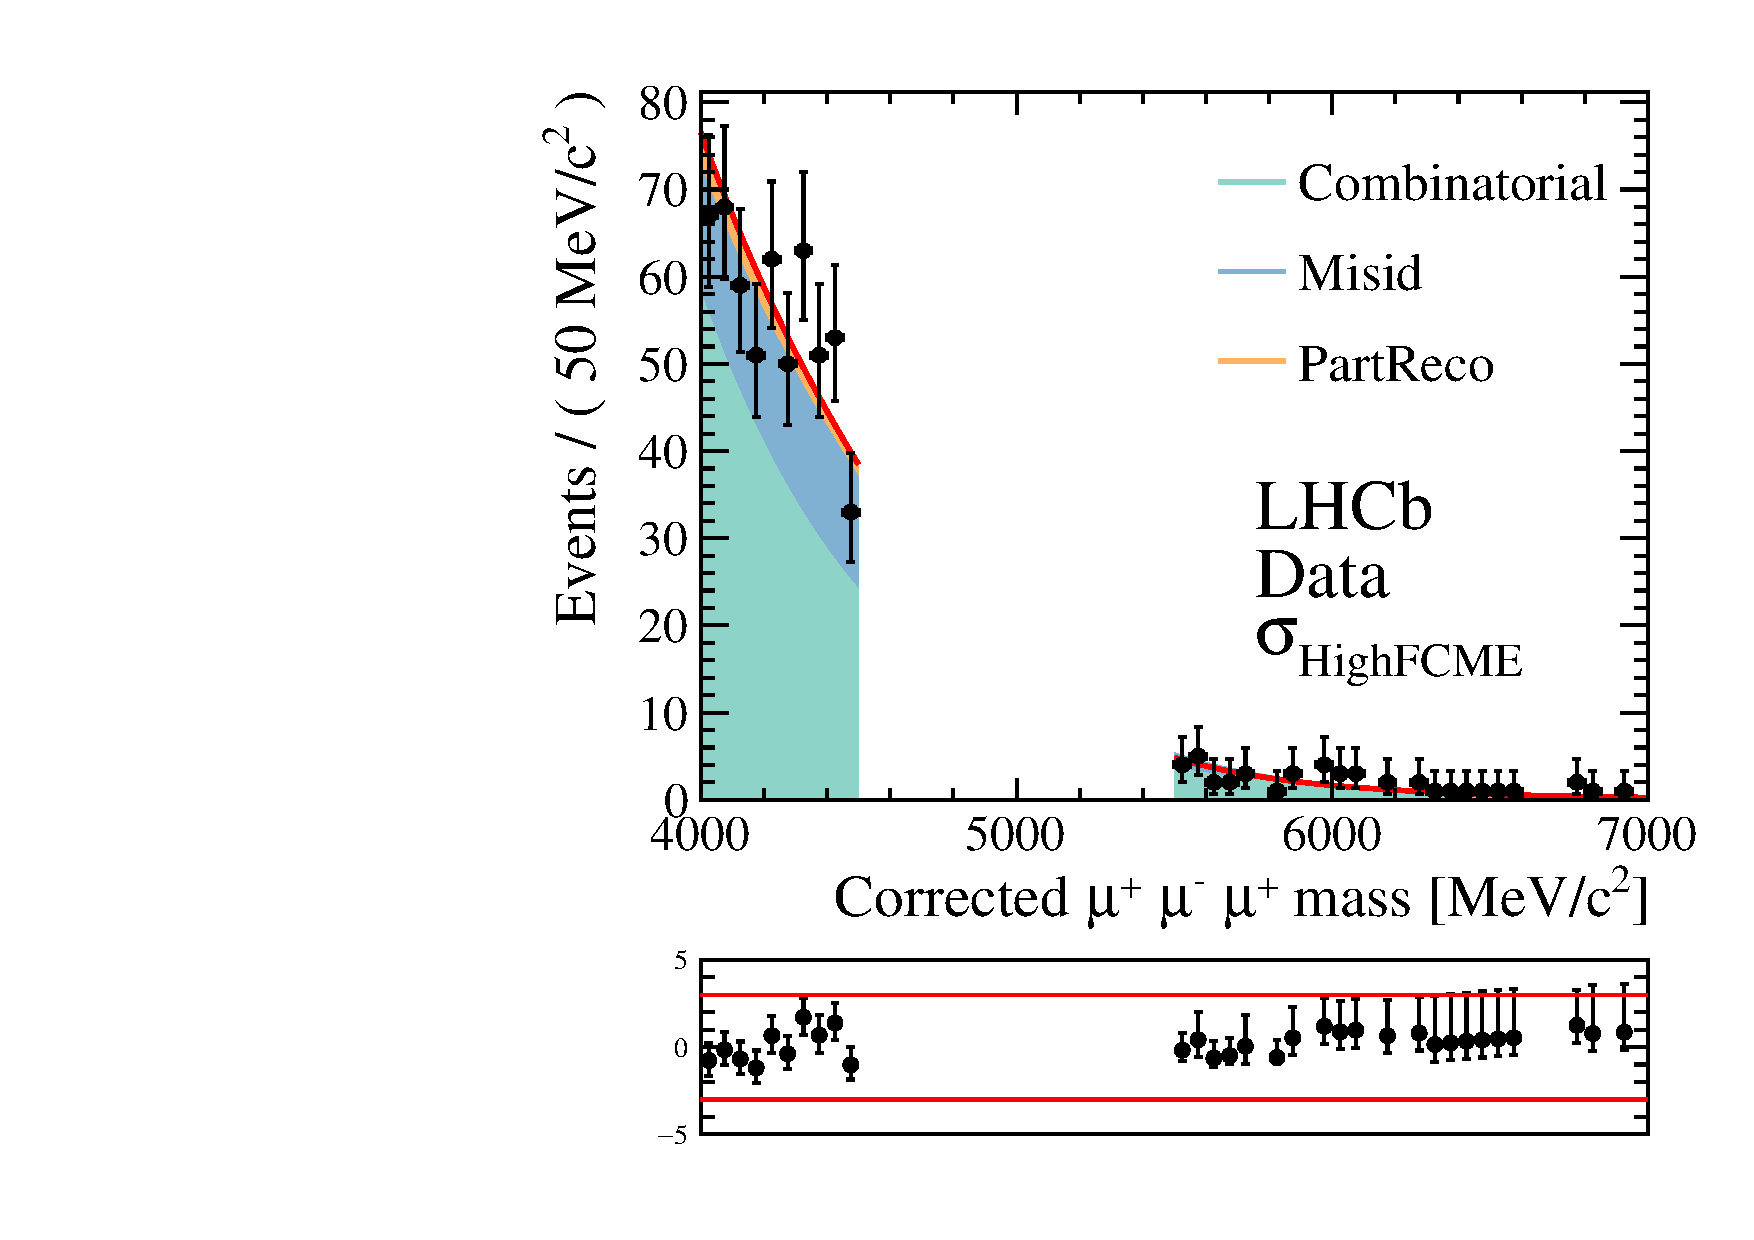
\includegraphics[width=0.5\linewidth]{./efficiency/blindedfits/HighFCMEprobnnmu035probmu35plotB23MuNuFitPretty_chi2_reallynice.pdf}\put(-30,100){(c)}%
\caption{(a) Unbinned maximum likelihood fit to the blinded data in one bin of FCME. Simultaneous unbinned maximum likelihood fit to blinded data after full selection chain in two bins of FCME, with (b) fit to $\sigma_{\mathrm{lowFCME}}$ bin, (c) $\sigma_{\mathrm{highFCME}}$ bin.}
\label{fig:sigfitpretty}
\end{figure}



\begin{table}[H]
\centering
%\small
\begin{tabular}{l l l H  H  H  l  l  }
\toprule
	&Fit Parameter & Status & $\sigma_{NOFCME}$ & $\sigma_{LowFCME}$ & $\sigma_{HighFCME}$  & Constraint & Obtained in  \\ \midrule

%        &\multicolumn{7}{c}{Yields} \\ \midrule 
%	& $N^{sig}$& Free & depend $\mathcal{B}$ & depend $\mathcal{B}$  & depend $\mathcal{B}$ & - & ~\autoref{eq:sigeq} \\ \midrule
        \ldelim\{{6}{0.3cm}[$N^{sig}$]& $ \mathcal{B}(\Bmumumu)$ & Free & & & & - & This Fit  \\  
	&	$ \mathcal{B}(\bjpsimumuk) $ & Cnstr. & & & & gaus. & ~\autoref{eq:normeq} \\  
	&	$ R^{21}_{\mathrm{FCME}}(\Bmumumu) $ & Cnstr. & & & & gaus. & ~\autoref{eq:nofcmeer}\\%/~\autoref{eq:allfcmeer} \\  
	&	$ R^{26}_{\mathrm{FCME}}(\Bmumumu) $ & Cnstr. & & & & gaus. & ~\autoref{eq:nofcmeer}\\%/~\autoref{eq:allfcmeer}  \\  
	&	$ N(\bjpsimumuk)^{Run \Rn{1}}_{\mathrm{FCME}} $ & Cnstr. & & & &  gaus. & ~\autoref{tab:normchannelyields} \\  
	&	$ N(\bjpsimumuk)^{2016}_{\mathrm{FCME}} $ & Cnstr. & & & &  gaus. & ~\autoref{tab:normchannelyields} \\ \midrule 
%	&	$N^{PR}$ & Cnstr. & 58.6$\pm$5.56& 32$\pm$3.05 & 25.3$\pm$2.49 &  gaus. &  ~\autoref{tab:prsum} \\ \midrule
	\ldelim\{{5}{0.7cm}[$N^{PR}$]&	$ \mathcal{B}(\pr) $ & Cnstr. & & & & gaus. & ~\autoref{tab:prsum} \\  
	&	$ \mathcal{B}(\bjpsimumuk) $ & Cnstr. & & & & gaus. & ~\autoref{eq:normeq} \\  
	&	$ R^{21}_{\mathrm{FCME}}(\pr) $ & Cnstr. & & & & gaus. & ~\autoref{tab:prsum} \\  
	&	$ N(\bjpsimumuk)^{Run \Rn{1}}_{\mathrm{FCME}} $ & Cnstr. & & & Cnstr. & gaus. & ~\autoref{tab:normchannelyields} \\  
	&	$ N(\bjpsimumuk)^{2016}_{\mathrm{FCME}} $ & Cnstr. & & & Cnstr. & gaus. & ~\autoref{tab:normchannelyields} \\ \midrule 
	&	$N^{Misid}$ & Cnstr. & 606 $\pm$26.8& 322 $\pm$16.9&  277 $\pm$15.5 & mvg$\_$gaus.  & ~\autoref{fig:MisidFinalFit}\\
	&	$N^{Combi}$ & Free & - & - & - & - &  This fit  \\ \hline
	&	\multicolumn{7}{c}{MisID Shape Parameters (Crystal Ball function)} \\ \midrule
	&	$\mu_{misid}$ & Cnstr.  & 4130 $\pm$150 & 4240 $\pm$74.7 & 4090 $\pm$143 & mvg$\_$gaus.  & ~\autoref{fig:MisidFinalFit}\\
	&	$\sigma_{misid}$ & Cnstr. & 566 $\pm$62 & 447 $\pm$35.9& 637 $\pm$61.9  & mvg$\_$gaus.   & ~\autoref{fig:MisidFinalFit}\\ 
	&	Others & Fixed & \multicolumn{4}{c}{}& {~\autoref{fig:MisidFinalFit}}\\ \midrule
	&	\multicolumn{7}{c}{PartReco Shape Parameters (sum of two Crystal Ball functions)} \\ \midrule
	&	All & Fixed & \multicolumn{4}{c}{} & {~\autoref{fig:PRFit}} \\ \midrule
	&	\multicolumn{7}{c}{Signal Shape Parameters (Double-sided Crystal Ball function)} \\ \midrule
	&	All & Fixed & \multicolumn{4}{c}{} & {~\autoref{fig:MCSignalFit}} \\ \midrule
	&	\multicolumn{7}{c}{Combinatorial Shape Parameters (exponential function)} \\ \midrule 
	&	$\beta$ & Free & - & -& - & - & This fit \\ \bottomrule
\end{tabular}
	\caption{For all constrained variables the range is set to be within $\pm 5 \sigma$. Cnstr. stands for constrained variables, gaus. for \textit{gaussian} constraint and mvg\_gaus. \textit{multivariate gaussian} constraint. }
\label{tab:floatingparsummary}
\end{table}



\subsection{Expected Sensitivity}
\label{sensitivity}
The $CL_{s}$ method\cite{Read:2002hq} is used to produce an expected upper limits from the blinded data fits. This is possible thanks to the fact that this method is based on generation of pseudo-datasets with different signal hypothesis. Therefore, it only requires the resulting PDFs of the blinded fits (simultaneous and non-simultaneous) with which pseudo-datasets can be produced.

Systematic uncertainties directly influence the relative efficiencies between signal and normalisation channel. They can therefore be added as gaussian constraints on the relevant efficiency ratio. The expected exclusion limits are then computed and summarized in~\autoref{tab:explimits}. Partial systematics only include systematics related to branching fractions, whereas full systematics include all the effects from~\autoref{tab:systematicsummary}. In simultaneous fit these effects are assumed to be 100\% correlated between the two bins of fractional corrected mass, but uncorrelated between themselves. As expected, the limit weakens with the addition of systematics. On the other hand there is an increase in expected limit by $20\%$ obtained with the use of the simultaneous fit compared to the non-simultaneous fit with the full systematics included. Addition of Run \Rn{2} data also improved the expected sensitivity of the search. 
%are used to generate two types of pseudo-datasets: background-only pseudo-datasets, and signal+background pseudo-datasets at different assumptions of the branching fractions. After this both types of pseudo-datasets are fitted with signal+background hypothesis and background hypothesis. Ratio of likelihoods, where the test statistics, ratio of likelihoods, for both bacgkround pseudo-datasets and signal ps

%This means that for a given branching fraction assumption $\mathcal{B}$:
%\begin{itemize}
%%\item Likelihood ratio $-2 log \frac {\mathcal{L}(s+b)}{\mathcal{L}(b)}$ is calculated, where $\mathcal{L}(s+b)$ is the likelihood function under signal and background hypothesis and $\mathcal{L}(b)$ is likelihood under background only hypothesis. 
%\item 1000 pseudo datasets with no signal injected are generated (background only hypothesis) and are denoted as data$_{bkg}$.
%\item 1000 pseudo datasets with a given signal branching fraction hypothesis injected are generated (signal+background hypothesis) and are denoted as data$_{sig}$.
%\item Likelihood ratio $-2 log \frac {\mathcal{L}(s+b)}{\mathcal{L}(b)}$ is defined, where $\mathcal{L}(s+b)$ is the likelihood function under signal and background hypothesis and $\mathcal{L}(b)$ is likelihood under background only hypothesis. 
%\item Fits with background only hypothesis and signal+background hypothesis are performed to both data$_{bkg}$ and data$_{sig}$. By extracting the likelihood ratio from these fits likelihood ratio distributions for signal, $\Delta LL_{sig}$, and background, $\Delta LL_{bkg}$, are obtained.  
%%\item Fit background hypothesis and signal+background hypothesis pdfs to both bkg$\_$data and sig$\_$data
%%\item Extract bkg$\_\Delta$LL distribution for test statistics and sig$\_\Delta$LL for test statistics under signal+background hypothesis
%\item The median of background $\Delta LL_{bkg}$ is identified.
%\item $CL_{b}$ is calculated by integrating $\Delta LL_{bkg}$ from the tail of the distribution to this median. In this case, $CL_{b}$ represents the probability to obtain a result less compatible with the signal than the observed one in the background-only hypothesis.
%\item $CL_{s+b}$ is calculated by integrating  $\Delta LL_{sig}$ from the tail to this median. $CL_{s+b}$ then represents the probability to obtain a result which is less compatible with the signal than the observed result, assuming the signal+background hypothesis.
%\item $CL_{s}$ then can be calculated as $CL_{s+b}$/$CL_b$.
%\end{itemize}


%\begin{figure}[H]
%\centering
%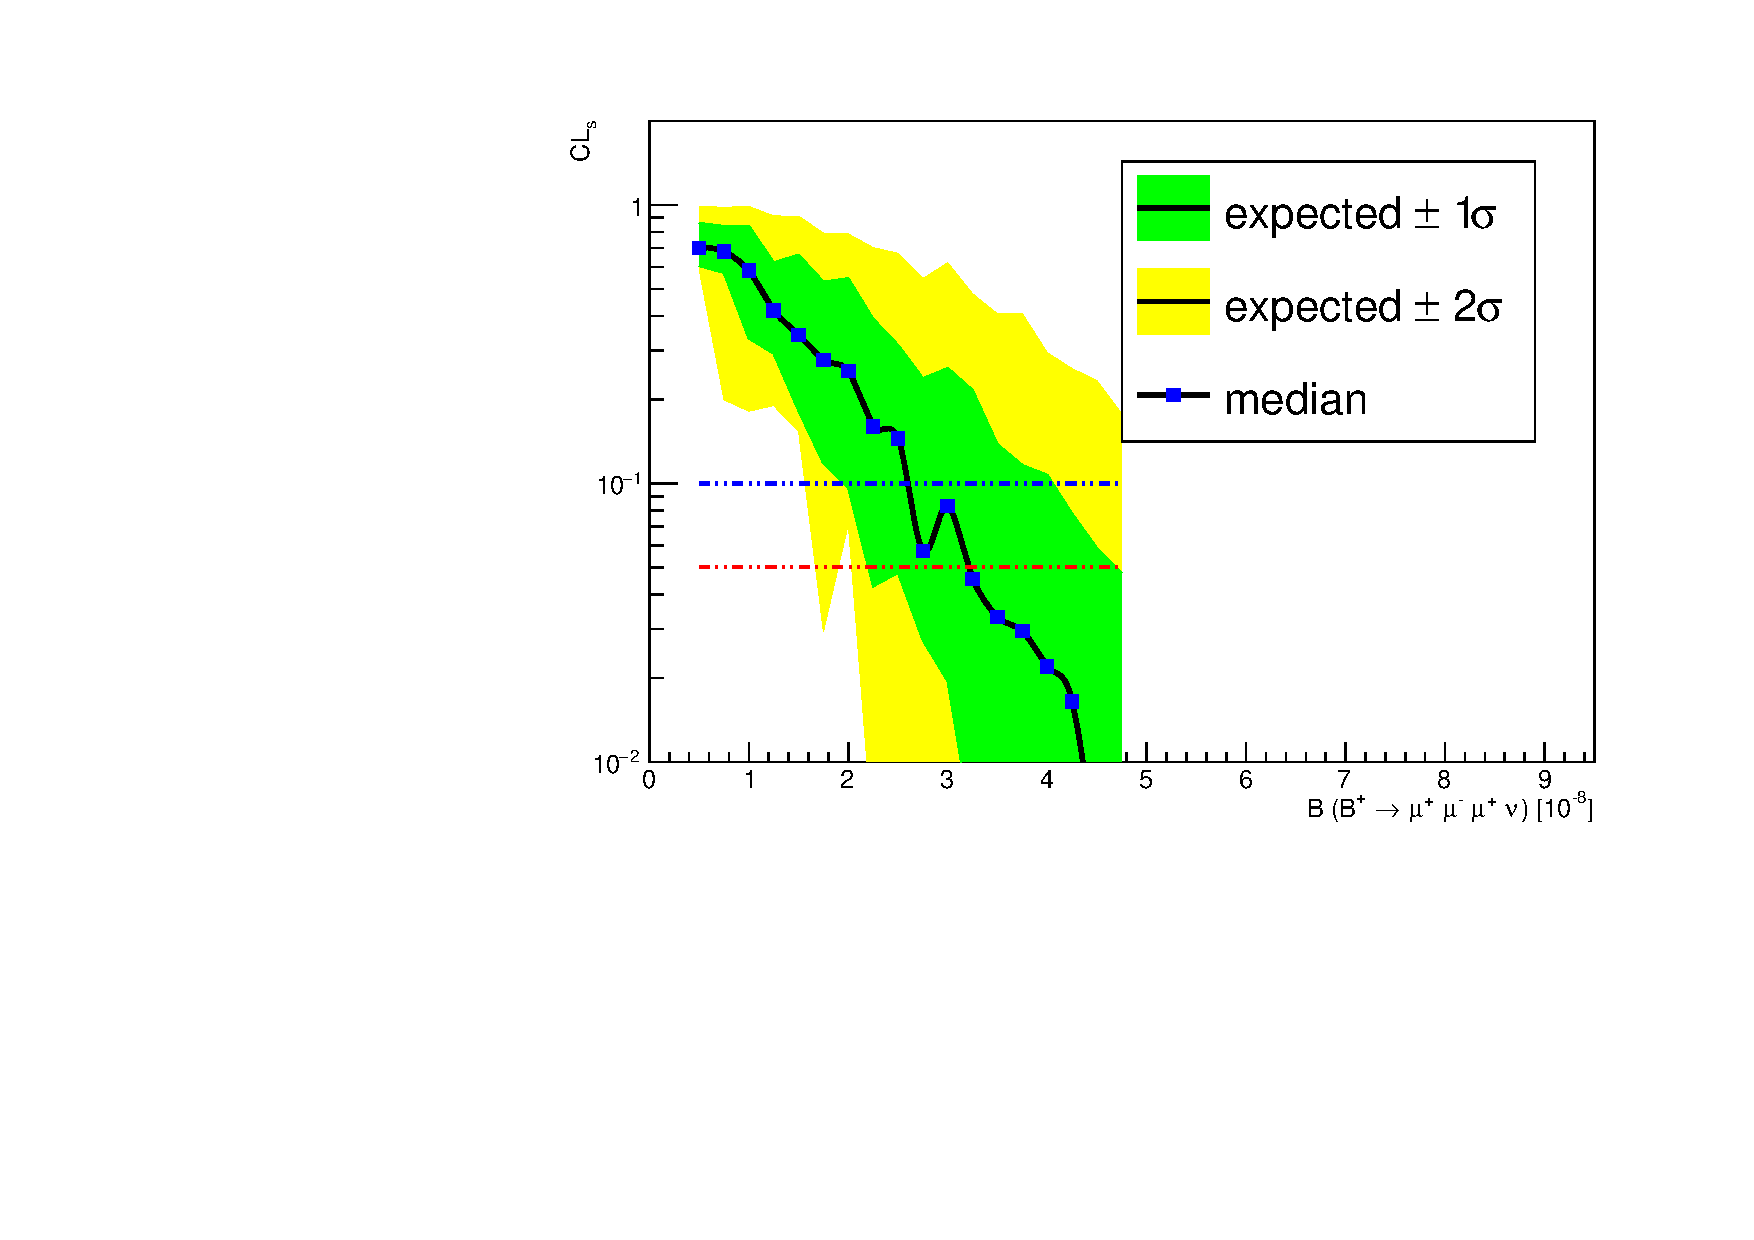
\includegraphics[width=0.5\linewidth]{./efficiency/expe_sensitivity/Run1onlySim_partial.pdf}\put(-75,30){(a) 3.25$\times$10$^{-8}$}%
%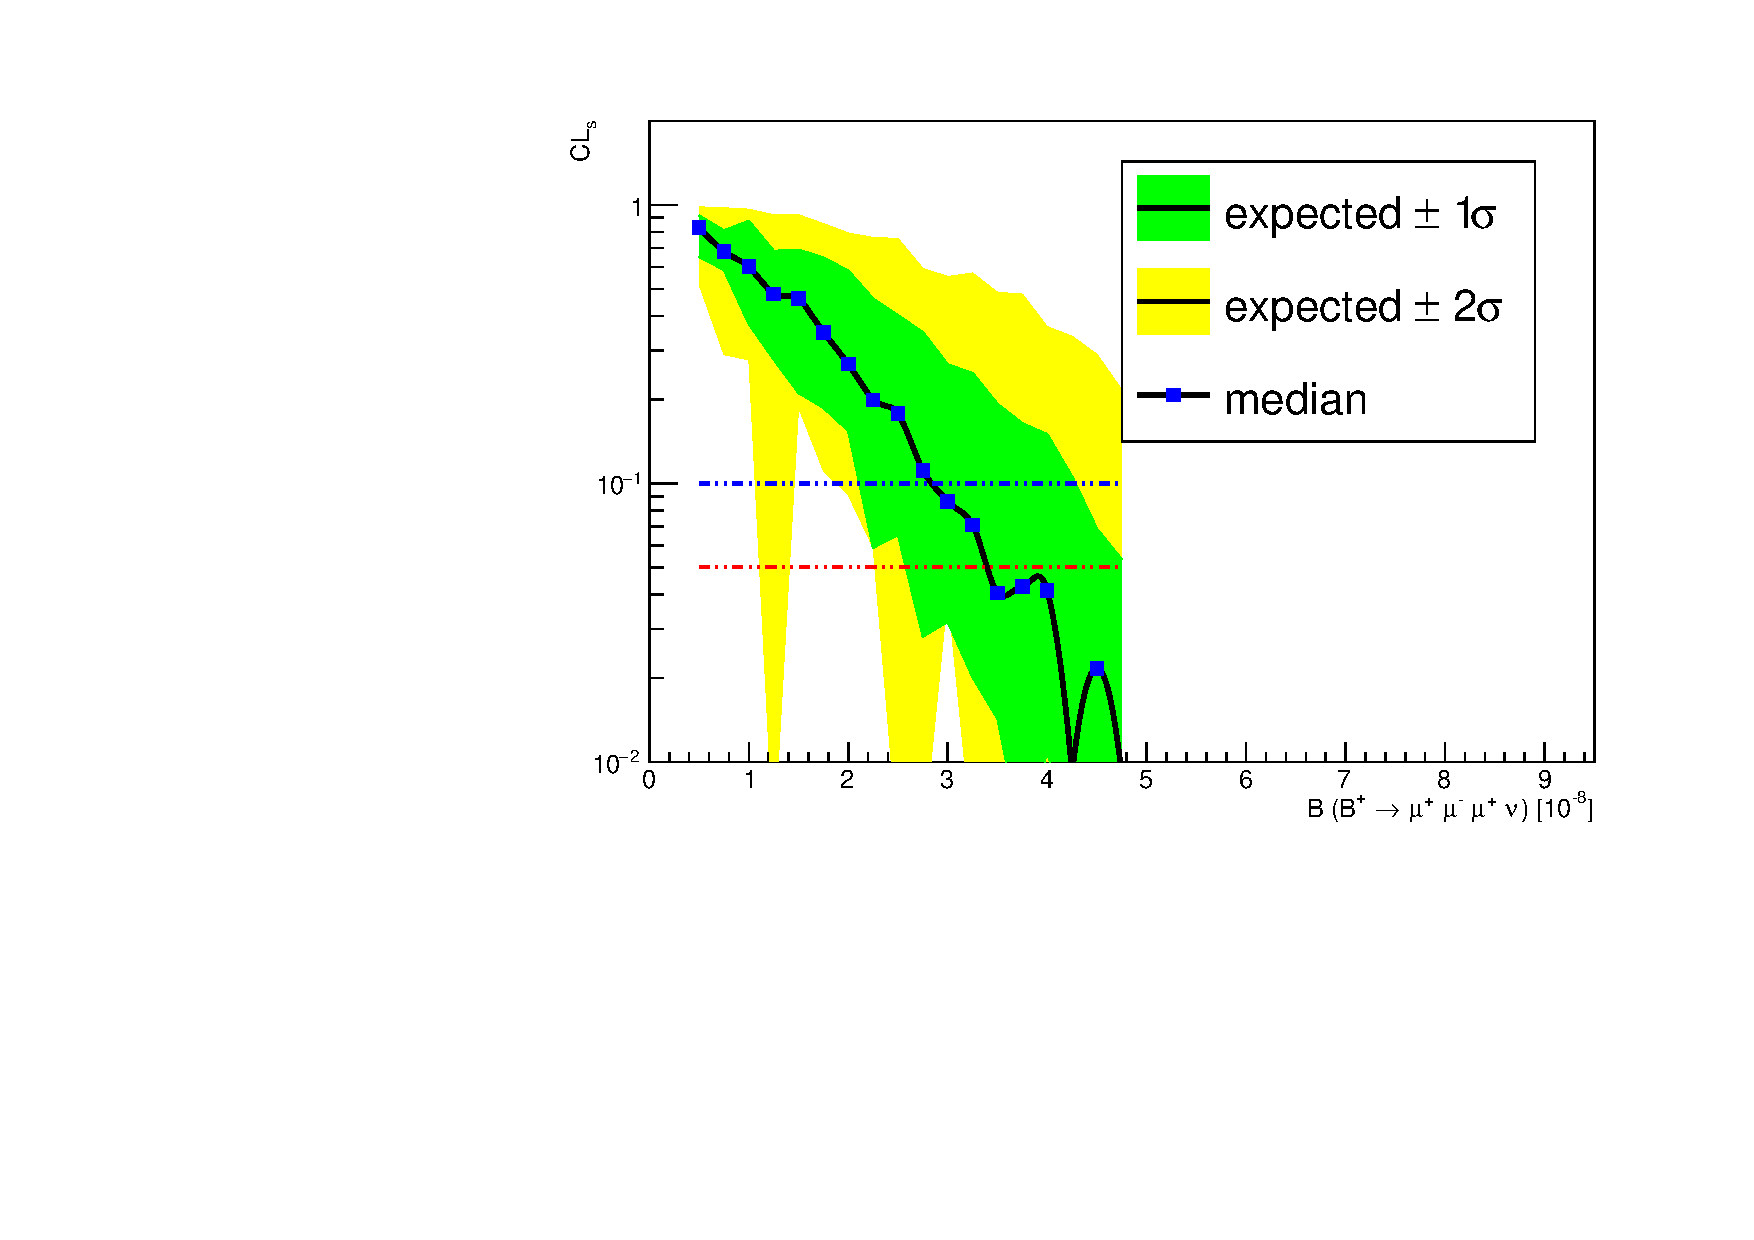
\includegraphics[width=0.5\linewidth]{./efficiency/expe_sensitivity/Run1onlySim_full.pdf}\put(-75,30){(b) 3.5$\times$10$^{-8}$}
%\newline
%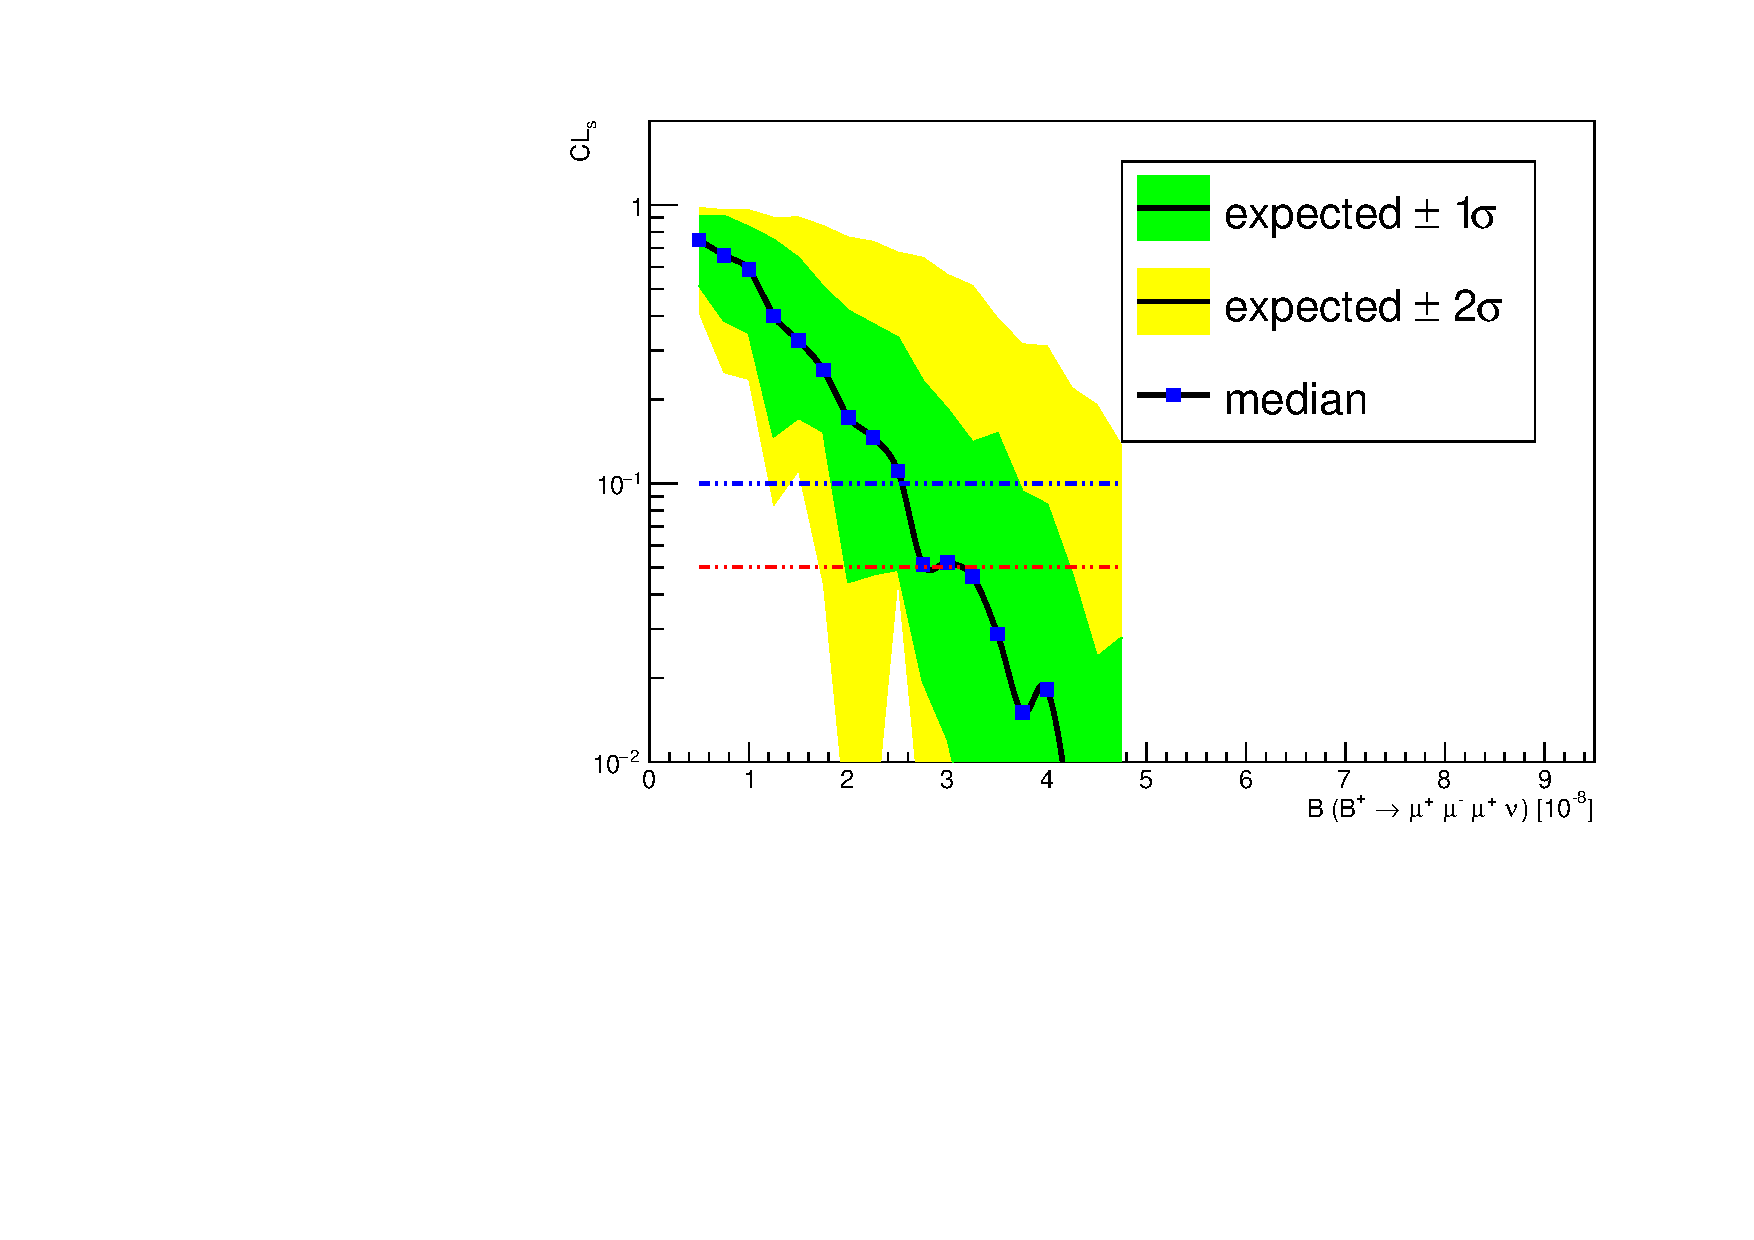
\includegraphics[width=0.5\linewidth]{./efficiency/expe_sensitivity/AllNotSim_partial.pdf}\put(-75,30){(c) 3.00$\times$10$^{-8}$}%
%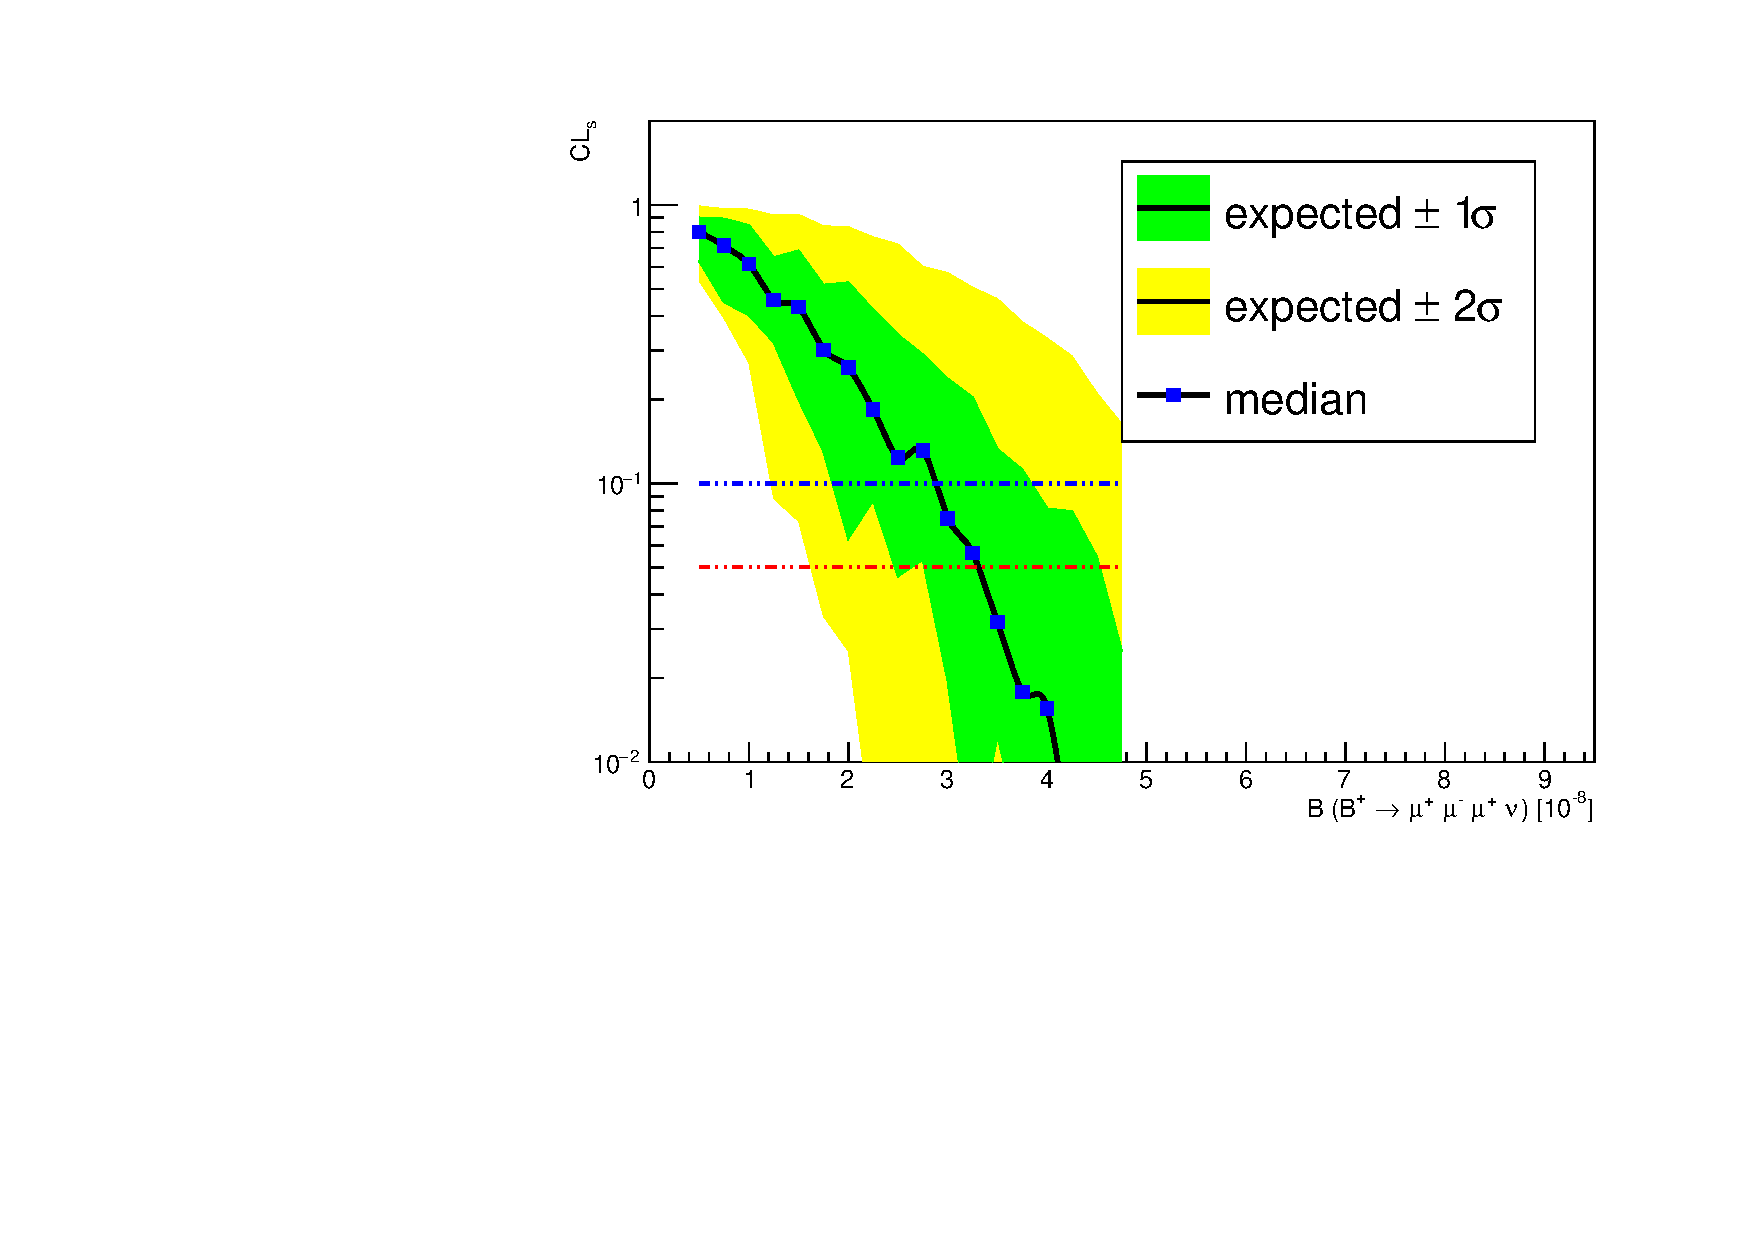
\includegraphics[width=0.5\linewidth]{./efficiency/expe_sensitivity/AllNotSim_full.pdf}\put(-75,30){(d) 3.25$\times$10$^{-8}$}
%\newline
%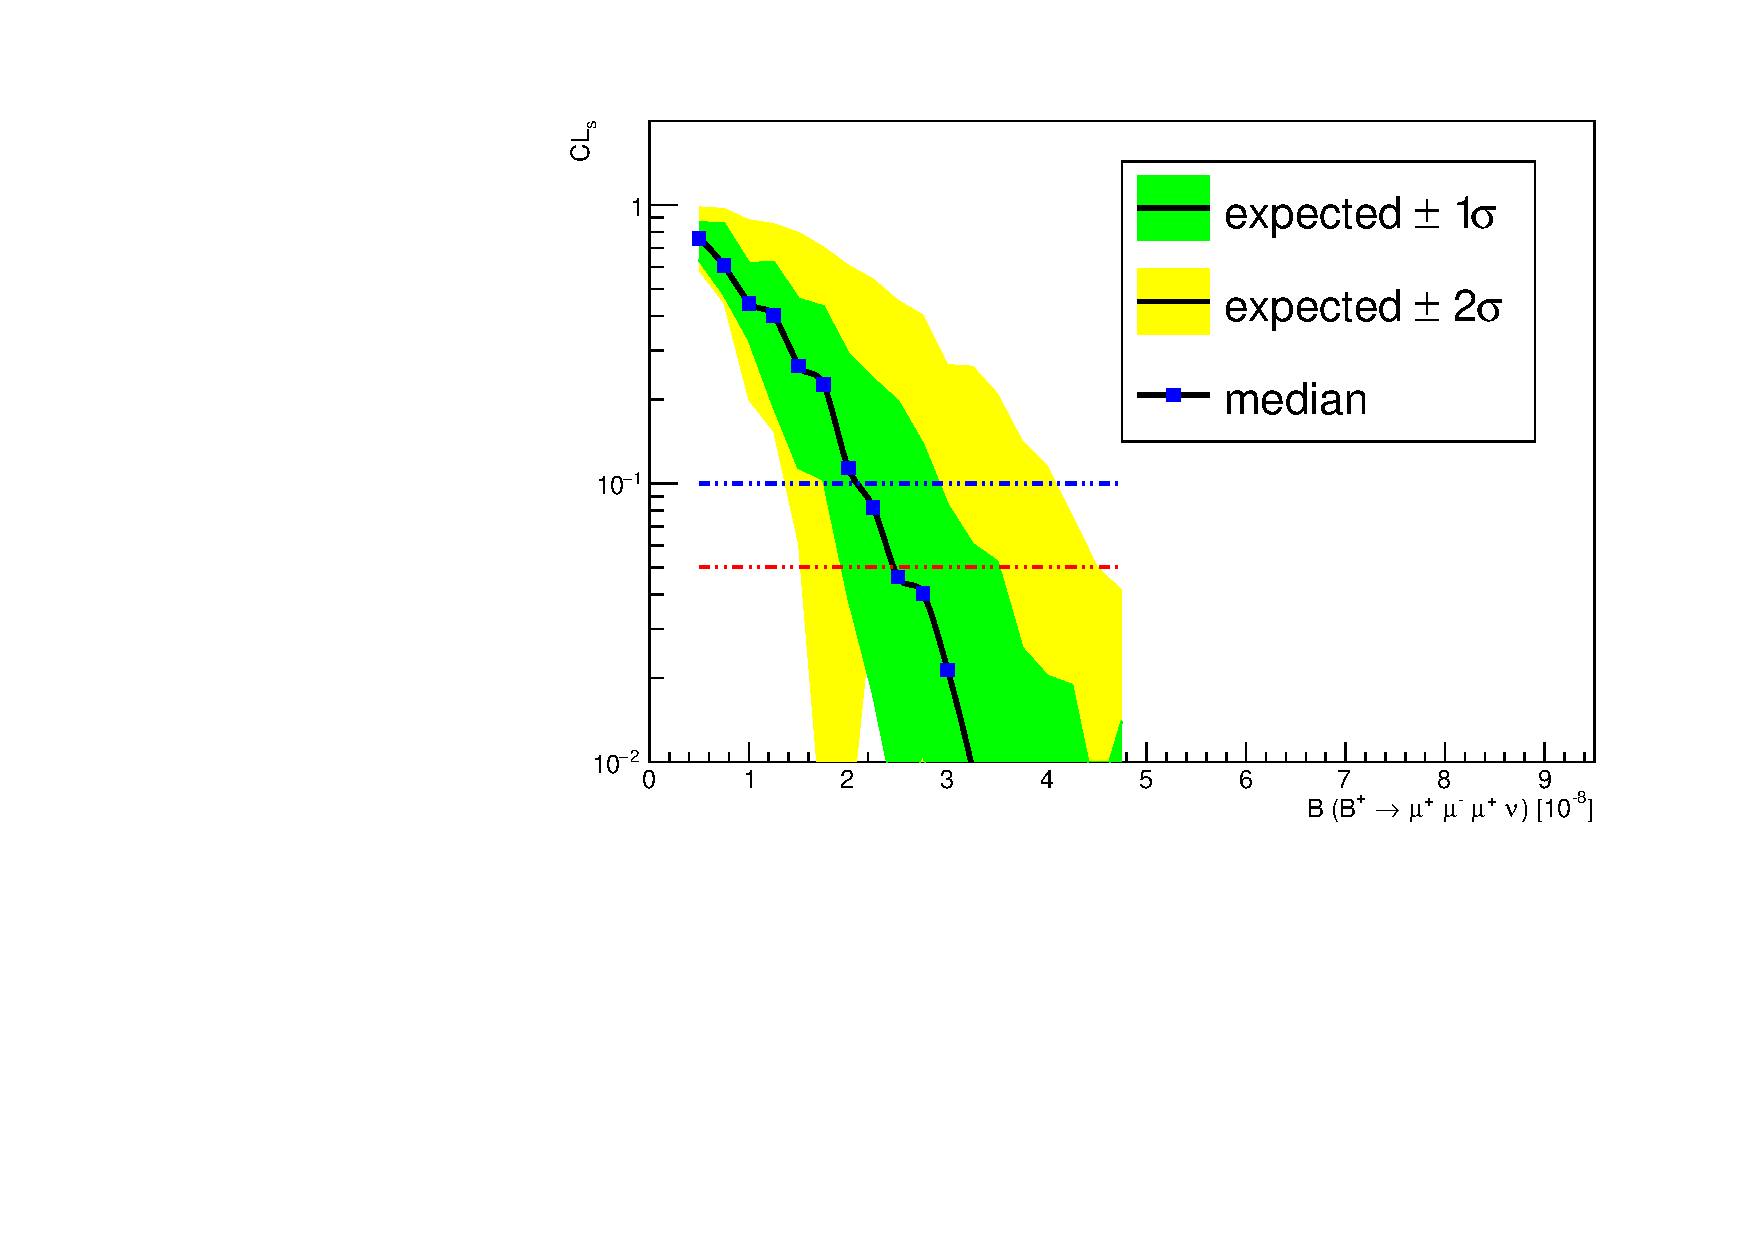
\includegraphics[width=0.5\linewidth]{./efficiency/expe_sensitivity/AllSim_partial.pdf}\put(-75,30){(e) 2.5$\times$10$^{-8}$}%
%\includegraphics[width=0.5\linewidth]{./efficiency/expe_sensitivity/AllSim_full.pdf}\put(-75,30){(f) 2.75$\times$10$^{-8}$}
%\caption{Expected 90\% (blue horizontal line) 95\% (red horizontal line) CL exclusion limits for full Run 1 data with simultaneous fit (a) with partial systematics and all statistical error constraints and (b) full systematics. Expected 90\% (blue horizontal line) 95\% (red horizontal line) CL exclusion limits for full Run 1 and 2016 data with non-simultaneous fit (c) with partial systematics and all statistical error constraints and (d) full systematics. And finally expected 90\% (blue horizontal line) 95\% (red horizontal line) CL exclusion limits for full Run 1 and 2016 data with simultaneous fit (e) with partial systematics and all statistical error constraints and (f) full systematics As expected full systematics sensitivity always yields slightly worse limits.}
%\label{fig:clsfit}
%\end{figure}
%


\begin{table}[H]
\centering
%\small
\begin{tabular}{ c  l  l  l  l  }
\toprule
Confidence & Data & Systematics & Fit Type & Value  \\ 
Interval & & & & \\ \hline
Expected $95\%$ CL & Run \Rn{1} & Partial & Simultaneous & $ 3.3\times 10^{-8}$ \\
Expected $95\%$ CL & Run \Rn{1} & Full & Simultaneous &$ 3.5\times 10^{-8}$ \\
Expected $95\%$ CL & Run \Rn{1} and \Rn{2} & Partial & Non-simultaneous & $ 3.0\times 10^{-8}$ \\
Expected $95\%$ CL & Run \Rn{1} and \Rn{2} &  Full & Non-simultaneous &$ 3.3\times 10^{-8}$ \\
Expected $95\%$ CL & Run \Rn{1} and \Rn{2} & Partial & Simultaneous & $ 2.5\times 10^{-8}$ \\
Expected $95\%$ CL & Run \Rn{1} and \Rn{2} &  Full & Simultaneous &$ 2.8\times 10^{-8}$ \\
\bottomrule
\end{tabular}
\caption{Resulting expected exclusion limits with both non-simultaneous and simultaneous fits. CL stands for confidence level.}
\label{tab:explimits}
\end{table}




\subsection{Unblinded Data Fits}
\label{unblindeddatafit}
After the full analysis strategy was reviewed the signal datasets were unblinded, observing no significant signal. The simultaneous unbinned extended maximum likelihood fit to all the data was performed. As expected with no excess signal, the background-only hypothesis fit described the data very well, which can be seen in~\autoref{fig:sigfit_unblinded_bkgonly}.

\begin{figure}[H]
\centering
\includegraphics[width=0.5\linewidth]{./efficiency/unblindedfits/LowFCMEprobnnmu035probmu35plotB23MuNuFitPretty_chi2_simPdfsig_with_0_reallynice.pdf}\put(-30,100){(a)}%
\includegraphics[width=0.5\linewidth]{./efficiency/unblindedfits/HighFCMEprobnnmu035probmu35plotB23MuNuFitPretty_chi2_simPdfsig_with_0_reallynice.pdf}\put(-30,100){(b)}%
\caption{Simultaneous unbinned extended maximum likelihood fit to unblinded data after full selection chain in two bins of FCME and with $\mathcal{B}=0$, with (b) fit to $\sigma_{\mathrm{lowFCME}}$ bin, (c) $\sigma_{\mathrm{highFCME}}$ bin.}
\label{fig:sigfit_unblinded_bkgonly}
\end{figure}

In order to perform fit with signal and background hypothesis a good range of the $\mathcal{B}$ needs to be established in order to aid the fit convergence. This is done the maximizing the log likelihood values for different values of $\mathcal{B}$, also known as profiling the $\mathcal{B}$. The results of the profiling can be seen in~\autoref{fig:prof}. This shows that the minimum is at $\mathcal{B}\sim-2.0\times10^{-8}$, hence the fit prefers a negative value of $\mathcal{B}$. 


\begin{figure}[H]
\centering
\includegraphics[width=0.6\linewidth]{./efficiency/unblindedfits/MyOwnProfileLL.pdf}%
\caption{Minimized -log likelihood value at different $\mathcal{B}$.}
\label{fig:prof}
\end{figure}

The simultaneous unbinned extended maximum likelihood fit to all the data with signal+background hypothesis is given in~\autoref{fig:sigfit_unblinded}, converging at value of $\mathcal{B}=-1.8\times10^{-8}$. This hence represents a negative yield fluctuation. The full list of all free and constrained parameters' values obtained in this fit is shown in~\autoref{tab:floatingparsummary_fit}. This fit result then can be translated into yields in all the fitting range and specifically blinded region by integrating the resulting PDF in a relevant region as shown in~\autoref{tab:yieldiatkos}.

\begin{figure}[H]
\centering
\includegraphics[width=0.5\linewidth]{./efficiency/unblindedfits/LowFCMEprobnnmu035probmu35plotB23MuNuFitPretty_chi2_simPdfsig_with__1_78461e_08_reallynice.pdf}\put(-30,100){(a)}%
\includegraphics[width=0.5\linewidth]{./efficiency/unblindedfits/HighFCMEprobnnmu035probmu35plotB23MuNuFitPretty_chi2_simPdfsig_with__1_78461e_08_reallynice.pdf}\put(-30,100){(b)}%
	\caption{Simultaneous unbinned maximum likelihood fit to unblinded data after full selection chain in two bins of FCME, with (b) fit to $\sigma_{\mathrm{lowFCME}}$ bin, (c) $\sigma_{\mathrm{highFCME}}$ bin. The signal component is visible as negative fluctuation.}
\label{fig:sigfit_unblinded}
\end{figure}

\begin{table}[H]
\centering
%\small
\begin{tabular}{ l  l  }
\toprule
Fit Parameter & Value  \\ \hline
$ \mathcal{B}(\Bmumumu) $ & $-1.8 \pm 0.9\times 10^{-8}$ \\
$ \mathcal{B}(\bjpsimumuk) $ & $(6.11 \pm 0.185)\times 10^{-5}$ \\
$ \mathcal{B}(\pr) $ & $(4.12 \pm 0.5)\times 10^{-7}$ \\
$ \mu_{misID_{\mathrm{highFCME}}} $ & $4100 \pm 123$ \\
$ \mu_{misID_{\mathrm{lowFCME}}} $ & $4330 \pm 56$ \\
$ \sigma_{misID_{\mathrm{highFCME}}} $ & $619 \pm 56$ \\
$ \sigma_{misID_{\mathrm{lowFCME}}} $ & $401 \pm 29.9$ \\
$ R^{26}_{\mathrm{highFCME}}(\Bmumumu) $ & $1.97 \pm 0.0788$ \\
$ R^{26}_{\mathrm{lowFCME}}(\Bmumumu) $ & $3.31 \pm 0.1$ \\
$ R^{21}_{\mathrm{highFCME}}(\pr) $ & $0.0397 \pm 0.00116$ \\
$ R^{21}_{\mathrm{lowFCME}}(\pr) $ & $0.0271 \pm 0.000794$ \\
$ R^{21}_{\mathrm{highFCME}}(\Bmumumu) $ & $1.96 \pm 0.131$ \\
$ R^{21}_{\mathrm{lowFCME}}(\Bmumumu) $ & $3.15 \pm 0.233$ \\
$ N(\bjpsimumuk)^{2016}_{\mathrm{highFCME}} $ & $29800 \pm 173$ \\
$ N(\bjpsimumuk)^{2016}_{\mathrm{lowFCME}} $ & $64700 \pm 254$ \\
$ N(\bjpsimumuk)^{Run 1}_{\mathrm{highFCME}} $ & $64100 \pm 253$ \\
$ N(\bjpsimumuk)^{Run 1}_{\mathrm{lowFCME}} $ & $109000 \pm 331$ \\
$ N^{scaled}_{misID_{\mathrm{highFCME}}} $ & $278 \pm 15.2$ \\
$ N^{scaled}_{misID_{\mathrm{lowFCME}}} $ & $331 \pm 16.3$ \\
$ \beta_{\mathrm{highFCME}} $ & $-0.00183 \pm 9.19\times 10^{-5}$ \\
$ \beta_{\mathrm{lowFCME}} $ & $-0.00226 \pm 0.000129$ \\
$ N_{combi_{\mathrm{highFCME}}} $ & $620 \pm 34.3$ \\
$ N_{combi_{\mathrm{lowFCME}}} $ & $531 \pm 35.4$ \\
\bottomrule
\end{tabular}
\caption{Fit results for all floating variables in the unblinded data fit. The $\mathcal{B}(\Bmumumu) =-1.8\times 10^{-8}$. Variables $R^{S}_{K}$ are the efficiency ratios obtained by normalising the decays to \bjpsimumuk decays where $S$ stands for stripping and $K$ for the FCME. $N^{scaled}_{misID_{K}}$ is the number of misID events, $N_{combi_{K}}$ is the number of combinatorial events, $\beta_{K}$ is the exponential constant, $\mu_{misID_{K}}$ and $\sigma_{misID_{K}}$ are the mean and the $\sigma$ of the CB function.}
\label{tab:floatingparsummary_fit}
\end{table}

\begin{table}[H]
\begin{center}
\begin{tabular}{ l  c  c }
\toprule
Component &  All ($4-7 \gevcc$) & Signal region ($4.5-5.5\gevcc$)  \\
\hline
$N_{misID_{\mathrm{lowFCME}}}$  &  331 & 139 \\
$N_{sig_{\mathrm{lowFCME}}}$  & -15.8  & -14.4 \\
$N_{combi_{\mathrm{lowFCME}}}$  & 531 & 154 \\
$N_{partreco_{\mathrm{lowFCME}}}$  & 31.8 & 6.39 \\
\hline
$N_{misID_{\mathrm{highFCME}}}$  &  279 & 122 \\
$N_{sig_{\mathrm{highFCME}}}$  &-14.0 & -11.0  \\
$N_{combi_{\mathrm{highFCME}}}$  & 620 & 209 \\
$N_{partreco_{\mathrm{highFCME}}}$ & 25.1 & 5.17 \\
\bottomrule
\end{tabular}
\end{center}
	\caption{Resulting yields for different components from the corrected mass fit with $\mathcal{B}(\Bmumumu) =-1.8\times 10^{-8}$.}
\label{tab:yieldiatkos}
\end{table}


